\documentclass[10pt, a4paper]{article}
\usepackage[backend=bibtex,style=numeric]{biblatex}
\usepackage[justification=centering]{caption}
\usepackage[pdfpagelabels,bookmarks,hyperindex,hyperfigures, hidelinks]{hyperref}
\usepackage[spanish,es-tabla]{babel}
\usepackage[toc, page]{appendix}
\usepackage[utf8]{inputenc}
\usepackage[version=4]{mhchem}
\usepackage{alltt}
\usepackage{amsmath}
\usepackage{booktabs}
\usepackage{circuitikz}
\usepackage{comment}
\usepackage{csquotes}
\usepackage{epstopdf}
\usepackage{fancyhdr}
\usepackage{gensymb}
\usepackage{hyphsubst}
\usepackage{lastpage}
\usepackage{multirow}
\usepackage{parskip}
\usepackage{pdfpages}
\usepackage{placeins}
\usepackage{subcaption}
\usepackage{tabularx}
\usepackage{textcomp}
\usepackage{tikz}
\usepackage{titlesec}
\usepackage{upgreek}
\usepackage{wrapfig}
\usepackage{xfrac}
\usepackage{pdfpages}

\usetikzlibrary{arrows, decorations.markings, positioning}
\addbibresource{major_paper.bib}

% if definition for section compilling control
\newif\ifdebug
%\debugtrue
\debugfalse

\setlength{\parskip}{0.6em}

% Set the indentation length 
\setlength{\parindent}{0em}


% Glossary entries
\usepackage[acronym, nomain]{glossaries}
\makenoidxglossaries

\newacronym{ABC}{ABC}{Active Balancing Controllers}
\newacronym{ACA}{ACA}{Advanced Control Algorithms}
\newacronym{ADC}{ADC}{Analog-to-digital converter}
\newacronym{AFE}{AFE}{Analog Frontend}
\newacronym{ANFIS}{ANFIS}{Adaptative Neuro-fuzzy Inference System}
\newacronym{ANN}{ANN}{Artificial Neural Network}
\newacronym{API}{API}{Application Programming Layer}
\newacronym{ARLB}{ARLB}{Aqueous Rechargeable Lithium Batteries}
\newacronym{ART}{ART}{Adaptive Real-Time Accelerator}
\newacronym{AVAE}{AVAE}{Average Value Equalization Algorithm}
\newacronym{BMS}{BMS}{Battery Management System}
\newacronym{C2C}{C2C}{cell-to-cell}
\newacronym{C2M}{C2M}{cell-to-module}
\newacronym{CAN}{CAN}{Controller Area Network}
\newacronym{CBBC}{CBBC}{Capacitor Based Balancing Controllers}
\newacronym{CBES}{CBES}{Capacity-based Equalization Strategy}
\newacronym{CCA}{CCA}{Classic Control Algorithms}
\newacronym{CC}{CC}{Constant Current}
\newacronym{CI}{CI}{Circuito Integrado}
\newacronym{CMSIS}{CMSIS}{Common Microcontroller Software Interface Standard}
\newacronym{CNN}{CNN}{Convolutional Neural Networks}
\newacronym{CRC}{CRC}{Cyclic Redundancy Check}
\newacronym{CV}{CV}{Constant Voltage}
\newacronym{CiA}{CiA}{CAN in AUTOMATION}
\newacronym{DB}{DB}{Diagrama de Bloques}
\newacronym{DMA}{DMA}{Direct Memory Access}
\newacronym{DMIPS}{DMIPS}{Dhrystone Million Instructions Per second}
\newacronym{DOD}{DOD}{Depth of Discharge}
\newacronym{DPM}{DPM}{}
\newacronym{DSP}{DSP}{Digital Signal Processor}
\newacronym{EC}{EC}{Eficiencia Culombica}
\newacronym{EIS}{EIS}{Electrochemical Impedance Spectroscopy}
\newacronym{EKF}{EKF}{Extended Kalman Filter}
\newacronym{EMI}{EMI}{Electromagnetic Interference}
\newacronym{EMS}{EMS}{Equalization Management System}
\newacronym{ESR}{ESR}{Equivalent Series Resistance}
\newacronym{EVEA}{EVEA}{Extreme Value Equalization Algorithm}
\newacronym{FIR}{FIR}{Finite Impulse Response}
\newacronym{FL}{FL}{Fuzzy Logic}
\newacronym{FOM}{FOM}{Figure-of-merit}
\newacronym{FPGA}{FPGA}{Field Programmable Gate Arrays}
\newacronym{FPU}{FPU}{Floating Point Unit}
\newacronym{GPIO}{GPIO}{General Purpose Input Output}
\newacronym{HAL}{HAL}{Hardware Abstraction Layer}
\newacronym{HPPC}{HPPC}{Hybrid Pulse Power Characterization}
\newacronym{HRI}{HRI}{Human-robot Interactions}
\newacronym{IBBC}{IBBC}{Inductor Based Balancing Controllers}
\newacronym{IC}{IC}{Integrated Circuit}
\newacronym{IISB}{IISB}{Institute for Integrated Systems and Device Technology}
\newacronym{Ion-Li}{Ion-Li}{Batería de Ion Litio}
\newacronym{KF}{KF}{Kalman Filter}
\newacronym{LIN}{LIN}{Local Interconnect Network}
\newacronym{LQFP}{LQFP}{Low-profile Quad Flat Package}
\newacronym{LSTM}{LSTM}{Long Short-Term Memory}
\newacronym{LUT}{LUT}{Look-up Table}
\newacronym{Li-Po}{Li-Po}{Batería de Polímero de Litio}
\newacronym{M2C}{M2C}{module-to-cell}
\newacronym{M2M}{M2M}{Module-to-Module}
\newacronym{MCU}{MCU}{Microcontroller Unit}
\newacronym{MLE}{MLE}{Maximum Likelihood Estimation}
\newacronym{ML}{ML}{Machine Learning}
\newacronym{MOST}{MOST}{Media Oriented Systems Transport}
\newacronym{MSE}{MSE}{Mean Squared Error}
\newacronym{NVIC}{NVIC}{Nested Vector Interrupt Controller}
\newacronym{OCV}{OCV}{Open Circuit Voltage}
\newacronym{OSI}{OSI}{Open Systems Interconnection}
\newacronym{OS}{OS}{Operative System}
\newacronym{OTP}{OTP}{One-Time-Programmable Memory}
\newacronym{PBBC}{PBBC}{Power Converter based Balancing Controllers}
\newacronym{PBC}{PBC}{Passive Balancing Controllers}
\newacronym{PCB}{PCB}{Printed Circuit Board}
\newacronym{PWM}{PWM}{Pulse-width Modulation}
\newacronym{RISC}{RISC}{Reduced Instruction Set Computer}
\newacronym{RNN}{RNN}{Recurrent Neural Network}
\newacronym{RTC}{RTC}{Real Time Clock}
\newacronym{SMT}{SMT}{Surface-Mount Technology}
\newacronym{SOA}{SOA}{Secure Operation Area}
\newacronym{SOC}{SoC}{State Of Charge}
\newacronym{SOH}{SoH}{State Of Health}
\newacronym{SPDT}{SPDT}{Single-Pole Double Throw}
\newacronym{SPST}{SPST}{Single-Pole Single Throw}
\newacronym{SRAM}{SRAM}{Static Random Access Memory}
\newacronym{SVM}{SVM}{Support Vector Machine}
\newacronym{SVN}{SVN}{Support Vector Machines}
\newacronym{SWD}{SWD}{Serial Wire Debug}
\newacronym{TBBC}{TBBC}{Transformer Based Balancing Controllers}
\newacronym{TCR}{TCR}{Temperature Coefficient of Resistance}
\newacronym{UPS}{UPS}{Uninterruptible Power Supply}
\newacronym{VBES}{VBES}{Voltage-based equalization strategy}
\newacronym{VE}{VE}{vehículo Eléctrico}
\newacronym{VVEE}{VVEE}{vehículos Eléctricos}
\newacronym{hri}{HRI}{Human-robot Interactions}


\tikzstyle{vecArrow} = [thick, decoration={markings,mark=at position
	1 with {\arrow[semithick]{open triangle 60}}},
double distance=1.4pt, shorten >= 5.5pt,
preaction = {decorate},
postaction = {draw,line width=1.4pt, white,shorten >= 4.5pt}]
\tikzstyle{innerWhite} = [semithick, white,line width=1.4pt, shorten >= 4.5pt]
\graphicspath{{assets/}} 
\newcommand\reaction[1]{\begin{equation}\ce{#1}\end{equation}} 

\titleclass{\subsubsubsection}{straight}[\subsection]

\newcounter{subsubsubsection}[subsubsection]
\renewcommand\thesubsubsubsection{\thesubsubsection.\arabic{subsubsubsection}}
\renewcommand\theparagraph{\thesubsubsubsection.\arabic{paragraph}} % optional; useful if paragraphs are to be numbered

\titleformat{\subsubsubsection}
  {\normalfont\normalsize\bfseries}{\thesubsubsubsection}{1em}{}
\titlespacing*{\subsubsubsection}
{0pt}{3.25ex plus 1ex minus .2ex}{1.5ex plus .2ex}

\makeatletter
\renewcommand\paragraph{\@startsection{paragraph}{5}{\z@}%
  {3.25ex \@plus1ex \@minus.2ex}%
  {-1em}%
  {\normalfont\normalsize\bfseries}}
\renewcommand\subparagraph{\@startsection{subparagraph}{6}{\parindent}%
  {3.25ex \@plus1ex \@minus .2ex}%
  {-1em}%
  {\normalfont\normalsize\bfseries}}
\def\toclevel@subsubsubsection{4}
\def\toclevel@paragraph{5}
\def\toclevel@paragraph{6}
\def\l@subsubsubsection{\@dottedtocline{4}{7em}{4em}}
\def\l@paragraph{\@dottedtocline{5}{10em}{5em}}
\def\l@subparagraph{\@dottedtocline{6}{14em}{6em}}
\makeatother

\setcounter{secnumdepth}{4}
\setcounter{tocdepth}{4}

\setcounter{MaxMatrixCols}{20}

\setlength{\headheight}{52pt}
\pagestyle{fancy}
\fancyheadoffset{0.5cm}
\fancyhead{}
\fancyhead[L]{
\includegraphics[scale=0.125]{FCEIA-logo.png}}
\fancyhead[C]{Universidad Nacional de Rosario\\
Facultad de Ciencias Exactas,Ingeniería y Agrimensura\\
Escuela de Ingeniería Electrónica}
\fancyhead[R]{
\includegraphics[scale=0.06]{LOGO-UNR-NEGRO.png}}

\renewcommand{\figurename}{Fig.}

\renewcommand\footrule{\begin{minipage}{0.95\textwidth}
    \hrule width \hsize   
\end{minipage}\par}

\setlength{\footskip}{30pt}
\fancyfoot[L]{\textit{Proyecto Final - F. Ceccarelli, M. Moya, L. Santos}}
\fancyfoot[C]{}
\fancyfoot[R]{\textit{Página \thepage{} de \pageref{LastPage}}}

\DeclareGraphicsExtensions{.bmp, .png, .jpg}

\renewcommand*\contentsname{Índice}

\topmargin = -1.5cm
\leftmargin = -1cm
\oddsidemargin = 0cm
\textheight = 24cm
\textwidth = 17cm

% renew itemize symbol level II
\renewcommand{\labelitemii}{$>$}

\begin{document}

\ifdebug
DebugOn
\newpage
\else
\begin{titlepage}
    \begin{center}
	\begin{minipage}{.45\textwidth}
	    \flushleft
	    
\includegraphics[scale=0.25]{FCEIA-logo.png}
	\end{minipage}%
	\hspace{20mm}
	\begin{minipage}{.3\textwidth}
	    \flushleft
	    
\includegraphics[scale=0.1]{LOGO-UNR-NEGRO.png}
	\end{minipage}

	\vspace{15mm}

	\large{ \textbf{Universidad Nacional de Rosario}} \\[5mm]
	\textbf{Facultad de Ciencias Exactas, Ingeniería y Agrimensura} \\[5mm]
	Escuela de Ingeniería Electrónica \\[20mm]
	\Large {\textbf{Área de Gestión de Proyectos}}\\[1.5mm]
	\small {Ingeniería Electrónica} \\[20mm]
	\Large {\textbf{Proyecto Final}} \\[5mm]
	\Large{ \textbf{Estudio e Implementación de un Sistema de Administración de
	Baterías de Li-Ion de baja y mediana potencia}} \\[15mm]

    \end{center}

    \begin{minipage}[t]{0.6\textwidth}
	{\large\textbf{Autores:}}
	\begin{itemize}
	    \item [] Federico Ceccarelli (C-6241/3)
	    \item [] Martin Moya (M-6132/8)
	    \item [] Lucio Santos (S-4966/2)
	\end{itemize}
	\vspace{10pt}
	{\large\textbf{Directora:}}

	\begin{itemize}
	    \item [] Dra. Monica Romero
	\end{itemize}
	\vspace{10pt}
	{\large\textbf{Asesor:}}
	\begin{itemize}
	    \item [] Ing. Edgardo Arnejo
	\end{itemize}
    \end{minipage}

    \begin{minipage}[t]{0.35\textwidth}
	\flushleft
	\Large\textbf{Firma:}
    \end{minipage}

\end{titlepage}

\newpage

\begin{abstract}

    \setlength{\parskip}{0.6em}

    \noindent En el presente trabajo se detalla el proceso de investigación,
    desarrollo e implementación de un administrador de baterías, tambien
    conocido como \acrshort{BMS} (del inglés \emph{\acrlong{BMS}}), compatible
    con un pack de bater\'ias de iones de litio.

    \noindent El dispositivo es capaz de:
    \begin{itemize}
        \item Estimar el estado de carga utilizando filtros cuadr\'aticos
        \item Cargar y balancear un pack de baterías de Ion-Litio
        \item Proteger el pack de baterías de Ion-Litio
        \item Comunicar, a trav\'es del protocolo \acrshort{CAN}, todas las
            variables del mismo.
    \end{itemize}

    \noindent Está orientado a veh\'iculos el\'ectricos de baja y mediana
    potencia, como por ejemplo, bicicletas/monopatines hasta triciclos de
    transporte con carga y busca resolver mucha de las problem\'aticas
    intr\'insecas de la tecnolog\'ia litio-ion, como por ejemplo, la
    inestabilidad del pack de batería frente a operaciones fuera del \'area
    segura de operaci\'on, como tambi\'en la falta de proyectos abiertos de esta
    \'indole en el mercado.

    \noindent A pesar de estar caracterizado para veh\'iculos el\'ectricos, el
    mismo puede ser aplicado a almacenadores de energ\'ia, tales como los
    paneles solares, incluso hasta sistemas de alimentaci\'on ininterrumpida, o
    \acrshort{UPS} (del inglés, \emph{\acrlong{UPS}}).

\end{abstract}

\newpage
% Print table of contents
\tableofcontents

\newpage

\section{Introducción}

\noindent A partir de la relevancia que ha comenzado a tomar el 
calentamiento global en las últimas décadas y el inquietante impacto que 
el mismo tiene sobre la calidad de vida de las personas, se han intentado 
buscar distintas soluciones para apaciguar las principales causas que 
generan un deterioro del medio ambiente, entre ellas, se encuentra el 
desarrollo de nuevas fuentes de energía renovables y su aprovechamiento.

\noindent El \acrfull{VE} \emph{(Fig. \ref{EV})} es considerado 
una de las transiciones tecnológicas más importantes de los últimos años 
debido a que no emiten dióxido de carbono ($\mathrm{CO_2}$) al medio 
ambiente y no utilizan combustibles fósiles para su funcionamiento, esto 
los convierte en uno de los avances tecnológicos más atractivos de los 
últimos tiempos teniendo en cuenta el avance del calentamiento global y el 
crecimiento del valor del petróleo.

\begin{figure}[h!]
    \begin{center}
	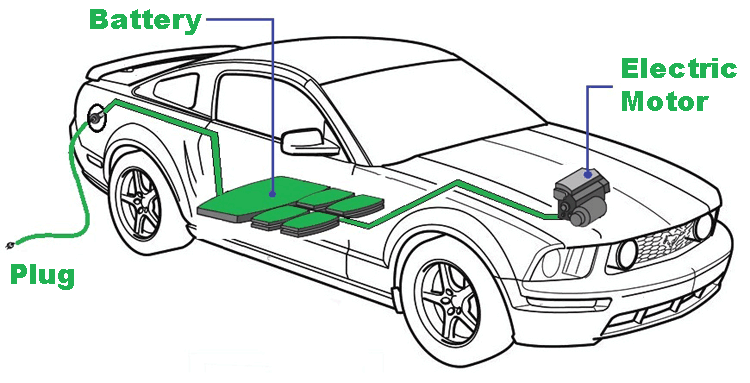
\includegraphics[width=0.7\textwidth]{EV.png}
	\caption{Esquem\'atico de un veh\'iculo electrico}
	\label{EV}
    \end{center}
\end{figure}

\noindent Siendo las baterías eléctricas la única fuente de energía en los 
\acrfull{VVEE}, éstas tienen un gran impacto en el desempeño de los mismos 
determinando la autonomía del vehículo. En base a este criterio, las 
baterías de iones de litio (\emph{Li-Ion}) resultan las más adecuadas para 
esta aplicación debido a su alta densidad energética, es decir, que este 
tipo de baterías tienen una gran capacidad para su reducido volumen a 
comparación de otras tecnologías. Para poder ser utilizados en
\acrshort{VVEE}, las baterías de Li-Ion son conectadas en forma de arreglos 
o packs de baterías en serie que permiten obtener mayores valores de tensión
y, otras, en paralelo para aumentar la capacidad del pack.

\subsection{Motivaci\'on del proyecto}

\noindent Una de las grandes problem\'aticas de las bater\'ias de Litio-ion 
reside en que se debe tener en cuenta ciertas precauciones a la hora de
implementarlas, debido a que las mismas son propensas a fallar al ser 
sobrecargadas, completamente descargadas u operadas fuera del
rango seguro de temperatura, tensi\'on o corriente, adem\'as, en un pack de 
bater\'ias conectadas en serie, se pueden manifestar pequeñas diferencias de 
capacidades a traves de todas las celdas, causado por tolerancias de
producci\'on o diferentes condiciones de operaci\'on, que tienden
a incrementar con cada ciclo de carga. Por \'ultimo, las bater\'ias
sufren un proceso de \emph{auto-descarga} (t\'ipicamente entre un
2-10\% dependiendo de la temperatura y el estado de carga de la misma). 
Si la distribuci\'on de temperatura a lo largo del pack es
heterog\'enea, las celdas con mayor temperatura tienden a una mayor
p\'erdida de capacidad provocando un desbalanceo de carga.
Esto trae varias consecuencias, entre ellas, se encuentran:

\begin{itemize}
    \item \textbf{Seguridad:} Si el voltaje máximo de carga es excedido por 
        unos cientos de milivoltios, puede provocar un embalamiento térmico, 
        derritiendo el pack de baterías y, por lo tanto, el dispositivo que 
        alimenta. En el peor de los casos puede explotar poniendo en riesgo el 
        bienestar del usuario.
    \item \textbf{Salud de la batería:} La degradación de la batería es 
        extremadamente sensible a la operación de la misma fuera de la zona 
        indicada. Si la temperatura de operación o la tensión máxima de carga 
        es excedida esto provoca una aceleración en la degradación de su vida 
        útil.
    \item \textbf{Autonomía:} Consideremos que el circuito de protección 
        detecta que una de las baterías se encuentra descargada a niveles 
        cercanos de operación insegura. En este caso, la protección frena la 
        descarga del pack por una sola celda y el resto se encuentran con 
        voltajes más altos y, por lo tanto, con un remanente de energía para 
        entregar a la carga desaprovechando la capacidad del pack entero.
\end{itemize}

Estas situaciones hacen necesario la implementación de un sistema de
administración de baterías (\emph{\acrshort{BMS}} por sus siglas en inglés
\acrlong{BMS}). En definitiva, un \acrshort{BMS} es un dispositivo encargado de
controlar las funciones vitales de las baterías para que operen de forma
correcta y segura, con el objetivo de otorgar seguridad al usuario y prolongar
la autonomía del vehículo. Las funciones más relevantes que llevan a cabo son:

\begin{itemize}
    \item Protección del pack para su operación en la región segura tanto 
        en tensión, corriente como también en temperatura.
    \item Ecualización de las celdas individuales del pack, es decir,
        controlar que la carga entre celdas sea uniforme
    \item Estimación del estado de carga del pack de batería 
        (\emph{\acrshort{SOC}} por sus siglas en ingl\'es \acrlong{SOC}).
    \item Estimación del estado de salud del pack de batería 
        (\emph{\acrshort{SOH}} por sus siglas en ingl\'es \acrlong{SOH}).
    \item Informar a la computadora central del vehículo los distintos 
        parámetros del pack de baterías.
\end{itemize}

\noindent Ademas de las problem\'aticas mencionadas anteriormente, en el mercado
actual se venden una gran variedad de \acrshort{BMS} con escasa documentaci\'on
sobre el mismo, dificultando su implementaci\'on con otros dispositivos, tales 
como computadoras centrales de veh\'iculos el\'ectricos hasta \acrshort{UPS}.

Por otro lado, existen solamente dos proyectos de c\'odigo/hardware abiertos
relacionados al desarrollo de \acrshort{BMS}, detallados a continuaci\'on.

\subsubsection{foxBMS}

\emph{foxBMS} \cite{foxbms} es un proyecto desarrollado por el Instituto de Sistemas
Integrados y Tecnolog\'ias de Dispositivos de la sociedad \emph{Fraunhofer} o
tambien llamado Fraunhofer IISB (del ingles \emph{\acrlong{IISB}}), una
organización de investigación alemana que comprende 72 institutos esparcidos por
todo el territorio alem\'an.

\noindent El desarrollo de este proyecto es el resultado de 15 años de
investigaci\'on en el \'area de energ\'ias renovables y es diseñado para 
administrar innovadores prototipos de sistemas de bater\'ias basados en la 
tecnolog\'ia iones de litio, desde pocas celdas conectadas en serie hasta 
centenares de kWh y kW, especialmente para sistemas que requieren altos niveles 
de fiabilidad.

\noindent El proyecto no tiene intenciones de ser usado de forma comercial en
productos ya que no cumple con estandards espec\'ificos y requieren determinados
certificados para ser vendidos en el mercado. Solamente cumple con el 
prop\'osito de ser una plataforma de ensayo y desarollo que provee todas las 
funcionalidades del manejo de la complejidad y tamaño de los sistemas de 
almacenamiento más avanzados al d\'ia de la fecha.

\noindent Si bien el mismo tiene extensa documentacion, originalmente fue
desarrollado para manejar packs de 12 a 18 celdas en serie, lo cual excede el
prop\'osito de la aplicaci\'on en cuestion por lo que no resulta viable para ser
implementado de forma directa. Tambien el hardware del proyecto es
extensivamente costoso y complejo, ya que implementa varios microcontroladores e
integrados dedicados hasta \acrshort{FPGA}s (del ingles, \emph{\acrlong{FPGA}}).

\subsubsection{openBMS}

A diferencia de \emph{foxBMS}, este proyecto fue desarrollado por ingenieros
independientes con el objetivo de diversificar los proyectos abiertos relativos
al tema en cuesti\'on.

\noindent El mismo busca desarrollar un \acrshort{BMS} capaz de manejar un
pack de bater\'ias de 4 a 96 celdas en serie, realizar el balanceo de las mismas 
y comunicar las variables del pack a traves del protocolo \acrshort{CAN}.

\noindent Si bien, se encuentran todos los archivos del proyecto a disposición
del publico, la documentaci\'on es muy escaza para ser implementado
f\'acilmente para un proyecto relacionado.

\noindent En definitiva, las motivaciones para llevar a cabo el presente trabajo
se basan en la complejidad en el manejo de grandes packs de
bater\'ias basadas en celdas de litio-ion y la falta de proyectos abiertos
disponibles relacionados al tema.

\subsection{Estructura del informe}

El informe se encuentra dividido en 6 secciones, en la Sección \ref{descripcion}
se realiza una descripci\'on en alto nivel del proyecto, detallando los
objetivos generales, las especificaciones y requerimientos del trabajo, a
continuaci\'on, se encuentra el fundamento te\'orico (Secci\'on \ref{teoria}),
donde se detalla el funcionamiento de una celda de litio-ion, los fundamentos
b\'asicos de modelados de celdas y algoritmos de estimaci\'on de carga, como
tambi\'en aquellos relacionados a la equalizaci\'on de celdas, adem\'as, se
presenta el desarrollo matem\'atico de mucho de los m\'etodos como tambi\'en una
comparativa, por ultimo se presentan las Secciones \ref{desarrollo} y
\ref{ensayos} donde se describe el desarrollo de la bater\'ia en si, en conjunto
con su modelo y algoritmos como tambi\'en su final implementaci\'on en un
sistema embebido con los ensayos realizados para validar el funcionamiento del
sistema. Finalmente, en la Secci\'on \ref{conclusiones} se describen las
conclusiones y futuros proyectos a continuar sobre el eje de estudio.

\section{Descripci\'on}\label{descripcion}

\subsection{Objetivos del proyecto}

Como solución a los problemas planteados, se propone desarrollar un
\acrshort{BMS} que cumpla con los siguientes requisitos:

\begin{itemize}
    \item Proteger el pack de baterías evitando que el mismo salga de su 
	zona de operación segura, tanto en tensión, corriente como en 
	temperatura, evaluando los umbrales correspondientes para las celdas de 
    Litio-Ion.
    \item Estimar el estado de carga en tiempo real.
    \item Balancear la carga entre celdas, priorizando el menor costo 
	energético posible del sistema y la mayor autonomía final del pack.
    \item Comunicar los parámetros fundamentales del pack a una computadora 
	central a través de algún protocolo estandarizado.
\end{itemize}

\noindent Para lograr estos objetivos, se plantea un estudio pormenorizado 
del estado del arte de la temática en cuestión procurando seleccionar las 
prácticas y metodologías más adecuadas para la solución del problema 
planteado, a partir de un estudio teórico. Finalmente se validará la 
solución elegida a partir de la implementación y ensayo de la solución 
desarrollada.

\subsection{Especificaciones}\label{proy_specs}

\noindent El sistema a implementar debe ser capaz de poder administrar un 
pack de bater\'ias de 6 m\'odulos conectados en serie, donde cada módulo est\'a 
compuesto por 3 celdas en paralelo encargado de: 

\begin{itemize}
    \item Sensar la tensión de las celdas individuales del pack y de la 
	corriente que circula desde y hacia el pack as\'i como tambi\'en 
	la temperatura media.
    \item Realizar el balanceo de los m\'odulos que componen a la bater\'ia.
    \item Proteger el mismo, desconectando el pack de bater\'ias de la carga
	frente a operaciones fuera de la zona segura.
    \item Estimar el estado de carga y detectar las celdas que se encuentran
	en desbalance utilizando una unidad de cómputo como por ejemplo, un
	microcontrolador o \acrshort{MCU} (del ingl\'es \emph{\acrlong{MCU}}).
    \item Controlar el proceso de carga del pack de bater\'ias.
    \item Comunicar las variables del sistema a una computadora central a
	trav\'es de un protocolo especificado
\end{itemize}

\noindent La descripción anterior se puede visualizar en el \acrfull{DB} de la
Figura \ref{bms}. Como puede observarse, el microcontrolador es el encargado de
comunicarse y comandar los módulos de protecci\'on, ecualizaci\'on y carga de 
la batería, como tambi\'en obtener variables de los mismos para poder estimar 
el \acrshort{SOC}, determinar el desbalanceo de una o m\'as celdas y tomar 
acci\'on al respecto, y por último, pero m\'as relevante, comandar las 
protecciones en caso de una falla y/o alerta de la batería. 
De forma simult\'anea, el mismo debe estar a cargo de comunicar las distintas 
variables del sistema a una computadora central.

\begin{figure}[h!]
    \begin{center}
	\begin{circuitikz}[european]
	    \draw (-4, -1) rectangle (-2, 1)[fill=blue!10!white];
	    \node at (-3, 0.2) {CPU};
	    \node at (-3, -0.2) {Central};
	    \draw [vecArrow] (-1.8, 0) to (-1, 0);
	    \draw [vecArrow] (-1.2, 0) to (-2, 0);

	    \draw (-1, -1) rectangle (1, 1)[fill=blue!10!white];
	    \node at (0, 0) {MCU};

	    \draw [blue,thin,dashed] (2.1, 2.5) rectangle (5.1, -2.5)[fill=blue!10!white];

	    \draw (2.2, 2.4) rectangle (5.0, 0.92)[fill=yellow!15!white];
	    \draw (2.2, 0.82) rectangle (5.0, -0.71)[fill=yellow!15!white];
	    \draw (2.2, -0.81) rectangle (5.0, -2.4)[fill=yellow!15!white];

	    \node at (3.6, 1.6) {Protección};           
	    \node at (3.6, -1.6) {Cargador};
	    \node at (3.6, 0) {Equalizaci\'on};
	    \draw [vecArrow] (1.2, 0) to (2.1, 0);
	    \draw [vecArrow] (1.5, 0) to (1, 0);

	    \draw (7, 2) -- (7, 2.2);
	    \draw (7, 2) to[battery1] (7, 1.6);
	    \draw (7, 1.4) -- (7, 1.6);
	    \draw (7, 1.4) to[battery1] (7, .9);            
	    \draw (7, .7) -- (7, .9);           
	    \draw (7, 0.7) to[battery1] (7, 0.2);           
	    \draw (7, 0.2) -- (7, -0.2);
	    \draw (7, -0.2) to[battery1] (7, -0.7);
	    \draw (7, -.7) -- (7, -.9);
	    \draw (7, -.9) to[battery1] (7, -1.4);
	    \draw (7, -1.4) -- (7, -1.6);
	    \draw (7, -1.6) to[battery1] (7, -2);
	    \draw (7, -2) -- (7, -2.2);

	    \draw (9, 2) -- (9, 2.2);
	    \draw (9, 2) to[battery1] (9, 1.6);
	    \draw (9, 1.4) -- (9, 1.6);
	    \draw (9, 1.4) to[battery1] (9, .9);            
	    \draw (9, .7) -- (9, .9);           
	    \draw (9, 0.7) to[battery1] (9, 0.2);           
	    \draw (9, 0.2) -- (9, -0.2);
	    \draw (9, -0.2) to[battery1] (9, -0.7);
	    \draw (9, -.7) -- (9, -.9);
	    \draw (9, -.9) to[battery1] (9, -1.4);
	    \draw (9, -1.4) -- (9, -1.6);
	    \draw (9, -1.6) to[battery1] (9, -2);
	    \draw (9, -2) -- (9, -2.2);

	    \draw (11, 2) -- (11, 2.2);
	    \draw (11, 2) to[battery1] (11, 1.6);
	    \draw (11, 1.4) -- (11, 1.6);
	    \draw (11, 1.4) to[battery1] (11, .9);          
	    \draw (11, .7) -- (11, .9);         
	    \draw (11, 0.7) to[battery1] (11, 0.2);     
	    \draw (11, 0.2) -- (11, -0.2);
	    \draw (11, -0.2) to[battery1] (11, -0.7);
	    \draw (11, -.7) -- (11, -.9);
	    \draw (11, -.9) to[battery1] (11, -1.4);
	    \draw (11, -1.4) -- (11, -1.6);
	    \draw (11, -1.6) to[battery1] (11, -2);
	    \draw (11, -2) -- (11, -2.2);

	    \draw (5.1, 0) to[short, -*] (7, 0);
	    \draw (7, 0) to[short, -*] (9, 0);
	    \draw (9, 0) to[short, -*] (11, 0);

	    \draw (7, 0.8) to[short, -*] (9, 0.8);
	    \draw (9, 0.8) to[short, -*] (11, 0.8);

	    \draw (7, 1.5) to[short, -*] (9, 1.5);
	    \draw (9, 1.5) to[short, -*] (11, 1.5);

	    \draw (7, 2.2) to[short, -*] (9, 2.2);
	    \draw (9, 2.2) to[short, -*] (11, 2.2);         

	    \draw (7, -0.8) to[short, -*] (9, -0.8);
	    \draw (9, -0.8) to[short, -*] (11, -0.8);

	    \draw (7, -1.5) to[short, -*] (9, -1.5);
	    \draw (9, -1.5) to[short, -*] (11, -1.5);

	    \draw (7, -2.2) to[short, -*] (9, -2.2);
	    \draw (9, -2.2) to[short, -*] (11, -2.2);           

	    \draw (5.1, 0.2) -- (6.2, 0.2) |- (7, 0.8) node at (7, .8){$\bullet$};
	    \draw (5.1, 0.4) -- (6, 0.4) |- (7, 1.5) node at (7, 1.5){$\bullet$};
	    \draw (5.1, 0.6) -- (5.8, 0.6) |- (7, 2.2) node at (7, 2.2){$\bullet$};

	    \draw (5.1, -0.2) -- (6.2, -0.2) |- (7, -0.8) node at (7, -.8){$\bullet$};
	    \draw (5.1, -0.4) -- (6, -0.4) |- (7, -1.5) node at (7, -1.5){$\bullet$};
	    \draw (5.1, -0.6) -- (5.8, -0.6) |- (7, -2.2) node at (7, -2.2){$\bullet$};

	    \draw [dashed] (-1.2, 2.6) rectangle (5.2, -2.6);
	    \draw node at (-.8, 2.8){BMS};

	    \draw [dashed] (6.5, 2.4) rectangle (11.5, -2.4);

	    \draw node at (8.2, 2.6) {Pack de Baterías 6s3p};

	    \draw (13, 1) to[R=$Z$] (13, -1);

	    \draw (11, 2.2) -- (12, 2.2)
	    |- (12, 1.5) -- (13, 1.5) |- (13,1) node at (12, 1.5){$\bullet$};

	    \draw (11, -2.2) -- (12, -2.2)
	    |- (12, -1.5) -- (13,-1.5) |- (13,-1) node at (12, -1.5){$\bullet$};

	    \draw node at (12.8, 1){+};
	    \draw node at (12.8, -1){-};  
	\end{circuitikz}
    \end{center}
    \caption{Diagrama en Bloques del \acrshort{BMS} y el pack de baterías}
    \label{bms}
\end{figure}

\section{Aspectos Te\'oricos}\label{teoria}


\subsection{Batería de Litio-Ion}

La energía eléctrica ha empoderado a la sociedad desde su descubrimiento y,
gracias a los avances tecnológicos, el acceso a la misma se vuelve cada vez más
sencillo y más eficiente incluso en las ubicaciones más remotas del planeta.
Sumado a eso, nos dirigimos a una sociedad que se aprovecha cada vez más de la
movilidad eléctrica a medida que la dependencia de una conexi\'on local es
menor.

En gran parte, estos desarrollos son posibles gracias al descubrimiento del
litio-ion y su aplicacion en baterías. Este tipo de batería ha revolucionado la
tecnolog\'ia en almacenamiento de energ\'ia y ha logrado impulsar la
revoluci\'on digital empoderando los dispositivos móviles, a trav\'es de su gran
capacidad y densidad energ\'etica.

\subsubsection{Principios b\'asicos}

El principio básico de funcionamiento de una batería, en su configuraci\'on
b\'asica, consiste en una celda compuesta por dos electrodos 
\emph{(Fig. \ref{batt_wk_ppl})}, cada una conectada a un circuito el\'ectrico, 
separado por un electrolito que es capaz de acomodar cargas dentro de sí. 
Frecuentemente, los electrodos son f\'isicamente separados por una barrera que 
previene que estén en contacto físico entre ellos, evitando así un corto 
circuito en la batería. En descarga, cuando la bater\'ia entrega corriente al 
circuito, toma lugar un proceso de oxidación en el electrodo negativo (\'anodo), 
resultando en un movimiento de electrones a trav\'es del circuito. Por el otro 
lado, en el electrodo positivo (c\'atodo), ocurre un proceso de reducción, 
reabastecido por los electrones del circuito. El voltaje de la celda depende 
fuertemente de la diferencia de potencial entre los electrodos, y del proceso 
espont\'aneo en su totalidad. Para baterías recargables el proceso puede ser 
reversible aplicando electricidad externa produciendo un proceso complementario 
de \emph{redox} (reducci\'on-oxidac\'on) en los electrodos. Este proceso es 
dependiente de la energ\'ia y es no espont\'aneo, es decir, que sucederá s\'i y 
solo s\'i un agente externo participa en el proceso.

\noindent En base a este principio de funcionamiento, surgen una gran variedad
de tecnologías, partiendo de la pila voltaica, hecha de dos discos de metales
distintos, uno de zinc y otro de cobre o plata, separados por un dieléctrico
(como cartón o cuero) sumergido en una solución electrolítica. Durante la
operación, el disco de zinc actua como ánodo, liberando electrones al circuito y
produciendo iones de metal (proceso de oxidación), mientras que la reacción en
el electrodo opuesto depende de las condiciones de trabajo. En presencia del
aire, el metal de cobre es parcialmente oxidado a CuO, y la reducción de CuO a
Cu se da en el electrodo. En la ausencia de aire, los protones en el electrolito
son reducidos a hidrógeno en la superficie del cobre. El voltaje de la celda es
de aproximadamente 0.8-1.1V, dependiendo de la exposición al aire. 
Esencialmente, la pila voltaica es una batería no recargable.

\begin{figure}[h!]
    \begin{center}
	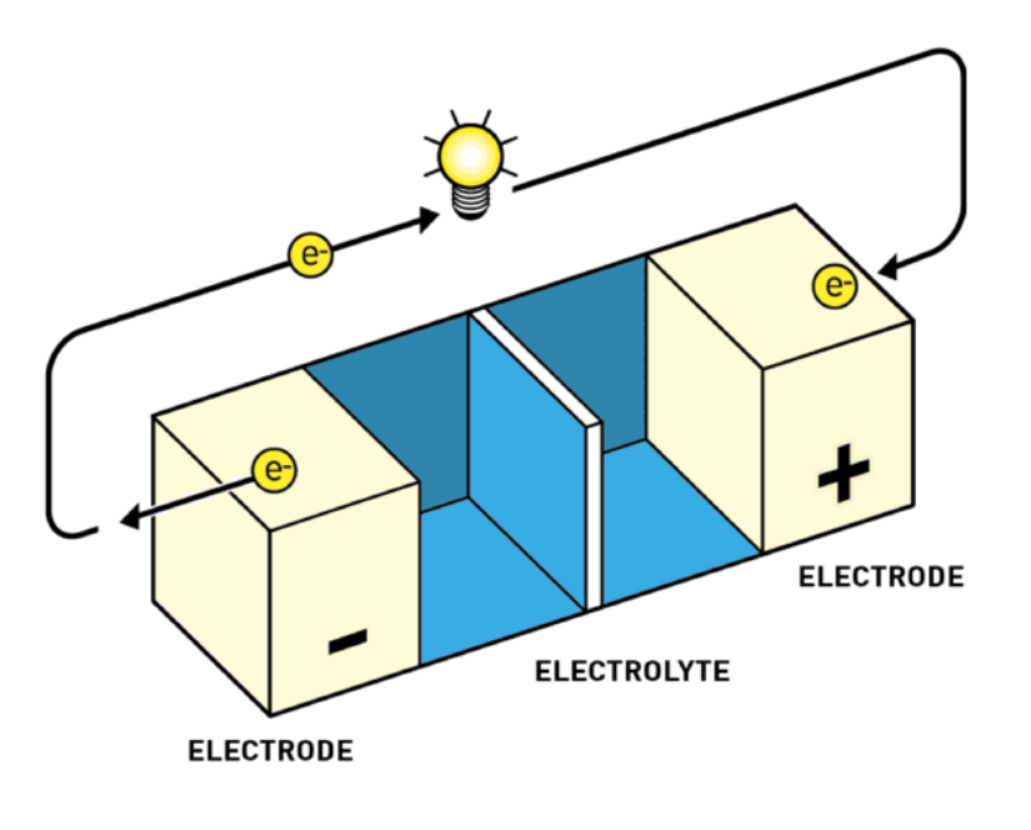
\includegraphics[width=0.4\textwidth]{batt_func_ppr.png}
    \end{center}
    \caption{Diagrama del principio básico de funcionamiento de una bater\'ia 
        en el proceso de descarga.}
    \label{batt_wk_ppl}
\end{figure}

\noindent Despu\'es surgieron las baterías de plomo-ácido, que su principio
de operaci\'on es similar a las baterías voltaicas expuestas al aire, pero con
la posibilidad de ser recargadas. Esta tecnología se basa en dos electrodos de
plomo, donde uno se encuentra parcialmente oxidado, en este caso es  oxido de 
plomo ($\mathrm{PbO_2}$), separado por \'acido sulf\'urico que contiene un 
electrolito. Durante el proceso de descarga, ocurre un proceso de oxidaci\'on 
en el electrodo de plomo (\'anodo), produciendo electrones, protones y sulfato 
de plomo ($\mathrm{PbSO_4}$), mientras que el \'oxido de plomo es reducido a
$\mathrm{PbSO_4}$ en el cátodo. En este caso, el potencial de una celda es de
alrededor 2V.

\noindent Otro logro en el desarrollo de baterías, ocurrió en el 1899 cuando se
desarrolló la primer batería de n\'iquel-hierro (Ni-Fe) y n\'iquel-cadmio
(Ni-Cd) o también conocidas como baterías alcalinas, que fueron predecedoras del
híbrido n\'iquel-metal (Ni-MH) que fue comercializada en 1898.

\noindent Las baterías anteriores son basadas en soluciones acuosas y la
densidad energética de las mismas no es alta, espec\'ificamente son menores a
los 100Wh/kg. Para incrementar la densidad energética de estas baterías, es
necesario encontrar una estabilidad electroquímica del agua ya que juega un rol
muy importante en ello. Además, es necesario buscar nuevos metales para
constituir los electrodos de las celdas ya que cuando \'ambos utilizan plomo,
debido al potencial del mismo, el voltaje de salida solo puede alcanzar un
máximo de 2.2V. Como resultado de los avances tecnol\'ogicos dentro del mercado
de consumo electr\'onico surge la necesidad de incrementar la densidad
energética de una celda, por lo tanto se impuls\'o la b\'usqueda de nuevas
tecnolog\'ias que permitan obtener una mayor capacidad en las bater\'ias con un
tamaño reducido, permitiendo el descubrimiento las propiedades del metal de
litio y su aplicacicación en las celdas que llevan su nombre.

\subsubsection{Litio}

El litio es un metal descubierto en 1818 que tiene excelentes propiedades para
servir como material para el desarrollo de baterías. Es el metal m\'as liviano
con una densidad de 0.53$\mathrm{g/cm^3}$. Tambi\'en tiene un potencial de
reducci\'on muy bajo, que lo hace ideal para celdas de alta densidad y alto
voltaje. Sin embargo, es un metal reactivo que debe ser protegido, por ejemplo,
del agua y del aire, ya que el contacto con estos provoca que el mismo sea muy
complicado de controlar, imposibilitando su uso para la aplicación deseada. Esta
protección al medio no es trivial, y factores, tales como su carácter inerte,
punto de fusión, la estabilidad del \emph{redox}, solubilidad de iones de litios
y sales, velocidades de transferencia ion/electrón, viscosidad, entre otros,
deben ser considerados.

\noindent Las primeras baterías de litio alcanzaron el mercado en 1970 y la
comercialización de las mismas comenzó en Japón en el año 1991, cuando
\emph{Sony Corporation} presentó el primer modelo.

\noindent Las baterías de litio-ion son definidas en \cite{Tatsuo2014} como
almacenadores de energía que utilizan iones de Litio como portadores de carga.
En base a esta definición, el término \emph{batería de Litio-Ion} no se
corresponde con una sola composición química, como lo son las baterías de ácido
o n'iquel-cadmio, si no que expresa una familia de baterías que dependen de los
iones de litio pero que pueden ser conformadas por distintos materiales.

%\newpage

\noindent A diferencia de las baterías de ácido, hay dos razones principales por
las cuales las baterías de litio-ion han crecido en popularidad en tan poco
tiempo: su excelente rendimiento y la capacidad de adaptarse al creciente
mercado de la electrónica de consumo, como por ejemplo, videograbadoras,
celulares y computadoras. A partir de la primer década del siglo XXI, se
comenzaron a utilizar en vehículos eléctricos, como también en grandes sistemas
de almacenamiento de energía, capaces de alimentar barrios residenciales
enteros.

\noindent Desde el 2000 al presente, se desarrollaron varios tipos de 
bater\'ias basadas en el litio. Entre ellas se encuentran las bater\'ias de 
litio-sulfuro (Li-S) y litio-aire (Li-air), cuya densidad energética teórica 
ronda los 2600Wh/kg y 11400 Wh/kg, respectivamente. En 2012, se desarrolló una 
batería de litio-ion recargable acuosa o \acrshort{ARLB} (del ingles
\emph{\acrlong{ARLB}}), que utiliza metal de litio recubierto como ánodo en una
solución de electrolitos mejorando ampliamente la densidad energética.

\subsubsection{Principio de funcionamiento}\label{battery_fun}

El principio de los procesos de carga y descarga en las baterías de litio-ion se
pueden describir utilizando como ejemplo el óxido de litio-cobalto 
($\mathrm{LiCoO_2}$) y grafito que son materiales de electrodo t\'ipicos en la
fabricaci\'on de las mismas. La Figura \ref{op_lithium-ion} ilustra el
princio de operación, y las reacciones de los electrodos se expresan en  las
Ecuaciones \ref{li_anode}, \ref{li_catode} y \ref{li_total}

\reaction{\text{Electrodo positivo: } LiCoO2 <=>[Carga][Descarga] Li_{1-x}CoO2 + xLi + xe^- \label{li_anode}}
\reaction{\text{Electrodo negativo: }6C + xLi^+ + xe^- <=>[Carga][Descarga] Li_{x}C6 \label{li_catode}}
\reaction{\text{Reaccion total: }6C + LiCoO2 <=>[Carga][Descarga] Li_{x}C6 + Li_{1-x}CoO2 \label{li_total}}

\noindent El \ce{LiCoO2} tiene una estructura reticular octa\'edrica con un
arreglo alternativo de capas de \ce{Li+} y \ce{Co^{3+}}. Durante el proceso de
carga, los iones de litio (en estado iónico) se desintercalan de la estructura
de capas del material del electrodo positivo, liberando electrones, al mismo
tiempo, el \ce{Co^{3+}} se oxida convirti\'endose en \ce{Co^{4+}}.  Por el otro
lado, durante el proceso de descarga, con la intercalación de \ce{Li+} dentro de
la ret\'icula, el \ce{Co^{4+}} es reducido a \ce{Co^{3+}}, ganando electrones,
adem\'as se obtienen electrones de la ret\'icula para convertirse en litio en 
estado atómico. Durante este proceso, el estado atómico del litio pierde 
electrones convirtiendose en iones de litio, este proceso se puede resumir en 
que el ánodo provee al electrodo positivo iones de litio. Dado que el litio se 
mueve entre el electrodo positivo y negativo hacia ambos lados a este tipo de 
baterías se las puede definir como una batería \emph{mecedora} (del ingles,
\emph{rocking chair}).

\begin{figure}[h!]
    \begin{center}
	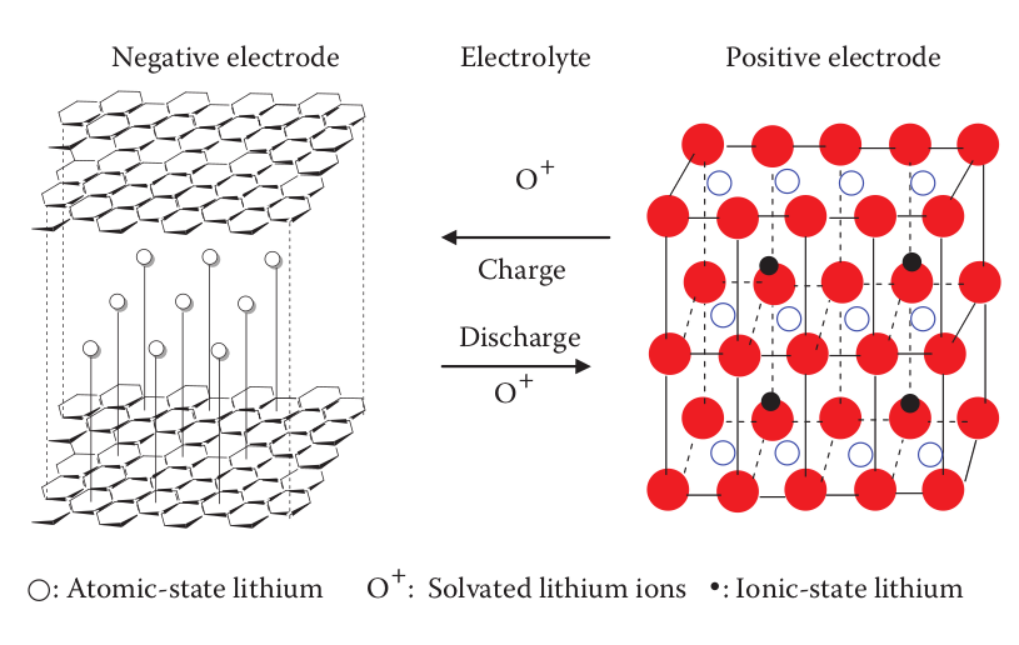
\includegraphics[width=0.7\textwidth]{prin_litio}
	\caption{Esquem\'atico del principio de operaci\'on de una bater\'ia de
	litio-ion.}
	\label{op_lithium-ion}
    \end{center}
\end{figure}

\noindent La mayoría de estas baterías usan materiales de carbón, tales como el
grafito o el carbón duro como ánodo. Otros utilizan óxidos de metales, como por
ejemplo, el titanato de litio ($\mathrm{Li_4Ti_5O_{12}}$) o el pentóxido de
niobio ($\mathrm{Nb_2O_5}$), debido a que pueden aceptar iones de litio cuando
son cargados, y liberarlos en el proceso de descarga, \'estas reacciones se
denominan como inserción y extracción respectivamente. Los potenciales de
reacción de estos materiales son mucho más bajos que los electrodos de hidrógeno
estándares, por lo tanto, el electrolito debería ser estable inclusive para
niveles de potencial tan bajos. Ésta es la razón por la cual, los electrolitos
orgánicos, que consisten de solventes orgánicos y sales de litio, son utilizados
en las baterías de Litio-ion en vez de electrolitos acuosos.

\noindent El material activo del cátodo debe contener Litio en su composición
química para proveer una fuente de iones de litio. Durante la primer etapa de
desarrollo de las celdas de litio, se utilizaba \'oxido de litio-cobalto.
También se estudió el uso de $\mathrm{LiNiO_2}$ (\'oxido de litio-nickel) como 
material activo para el cátodo pero fue inmediatamente descartado debido a su 
inestabilidad térmica. Sin embargo, se desarrollaron y utilizaron derivativos de 
esta composición, formulados como $\mathrm{LiM_xNi_{1-x}O_2}$  
(M: elemento metálico tales como, el cobalto, manganeso, aluminio o magnesio).

\newpage

\noindent Comparada con las baterías de litio-ion originales en los principios 
de 1990, el rendimiento de las mismas ha mejorado, de forma significativa, con 
el paso del tiempo. Los últimos desarrollos tienen ventajas dominantes sobre 
las baterías recargables tradicionales:

\begin{itemize}
    \item \textbf{Alta densidad energética:} La densidad energética por
	volumen y masa para una batería de litio modelo 18650 puede alcanzar
	los 500 Wh/$\mathrm{dm^3}$ y 230 Wh/kg, respectivamente, que adem\'as
	se encuentra en continuo aumento a medida que se investigan y
	desarrollan nuevas tecnologías.
    \item \textbf{Alto voltaje de salida (3.6V):} Esto es 3 veces 
        mayor a las baterías recargables de Ni-Cd o Ni-MH.
    \item \textbf{Alta potencia de salida:} Pueden alcanzar hasta 2kW/kg for
	un corto per\'iodo de tiempo.
    \item \textbf{Baja auto-descarga:} La descarga media de las celdas de
	litio son menores a un 3\% mensuales, que es la mitad que las celdas
	basadas en Ni-Cd y Ni-MH.
    \item \textbf{Bajo efecto de histéresis} A diferencia de las celdas de
	Ni-Cd y Ni-MH las celdas de litio tienen un efecto de histéresis
	despreciable con el paso de los ciclos de carga-descarga de la
	misma, resultando en un mejor ciclo de vida con respecto a los otros
	tipos de celdas.
    \item \textbf{Ciclos de carga-descarga rápidos:} Las baterías de
	litio-ion pueden ser cargadas con corrientes de hasta un 80\% de su
	capacidad. Es decir, si la batería tiene una capacidad de 3Ah, la
	misma se puede cargar a una corriente de 3A.
    \item \textbf{Alta eficiencia cul\'ombica:} La \acrlong{EC} o \acrshort{EC},
	es un par\'ametro que permite obtener que porcentaje del material
	activo se convierte en energia. Su medici\'on es importante porque 
	permite medir el desempeño de la bater\'ia con respecto a otras 
    tecnologias. En el caso de las celdas de Litio-ion, la \acrlong{EC}
	se mantiene casi en un 100\% inclusive despues del primer ciclo.
    \item \textbf{Gran rango de temperaturas}: Las bater\'ias de litio-ion
	pueden operar entre -25\degree C a +45\degree C. Las
	investigaciones actuales quieren extender ese rango desde -40\degree C a 
    +70\degree C con mejoras en el electrolito y los materiales de los 
    electrodos.
    \item \textbf{Alta energ\'ia espec\'ifica}: Esto depende fuertemente del alto 
    voltaje, porque la energía específica es el producto del voltaje de la celda 
    y su capacidad específica, lo que hace que las celdas de litio-ion se 
    destaquen a comparación de otras tecnologías, como por ejemplo, las celdas 
    de Niquel-metal con un voltaje de 1.2V pero con mayor capacidad tienen menor 
    energía específica. 
    \item \textbf{Alta eficiencia energética:} Esto se debe a dos 
	factores principales, por un lado se debe a la alta eficiencia de 
	carga y descarga debido a que no hay pérdidas durante las reacciones 
	químicas de la celda en ambos procesos y, nuevamente, esto se atribuye 
	también a su alto voltaje. Éste último, se debe a que la eficiencia 
	energética, es el restante de la tensión operativa en relación a la 
	tensión en circuito abierto. Suponiendo que tenemos una celda A con una 
	tensión de circuito abierto ($\mathrm{V_A}$) mayor que otra celda B con 
	una tensión $\mathrm{V_B}$, que tiene la misma pérdida de voltaje X, 
	la eficiencia de A va a ser mayor que la de B, dado por:
	\vspace{5mm}
	\begin{equation}
	    \frac{V_A - X}{V_A} > \frac{V_B - X}{V_B} \nonumber
	\end{equation}
    \item \textbf{Larga duración:} Esto se atribuye a que las reacciones 
	dentro de la celda, durante los ciclos de carga y descarga, no realizan 
	cambios morfológicos significativos. Esto es bastante distinto con las 
	baterías de ácido, donde la reacción que se lleva a cabo involucra la 
	disolución y deposición de materiales, lo que representa grandes 
	cambios morfológicos durante los ciclos de carga y descarga.
\end{itemize}

\noindent Por último, las baterías de Litio-ion utilizan electrolitos orgánicos.
El electrolito permite que la celda tenga altos niveles de tensión, sin embargo
la combustibilidad del mismo genera problemas de seguridad. Por lo tanto, es
clave para el desarrollo de estas baterías minimizar la causa y efecto de la
combustión de la misma sin sacrificar rendimiento.

\noindent El estado de las baterías de Litio-ion con respecto a las otras
tecnologías se puede observar en la Figura \ref{comparisson_batt}, donde se
remarca la dominancia de las mismas en términos de densidad energética (Wh/L) y 
energía específica (Wh/kg). La flecha de la esquina derecha indica que ésta 
tecnología se encuentra en constante desarrollo y puede mejorar con el paso del 
tiempo.

\begin{figure}[h!]
    \begin{center}
	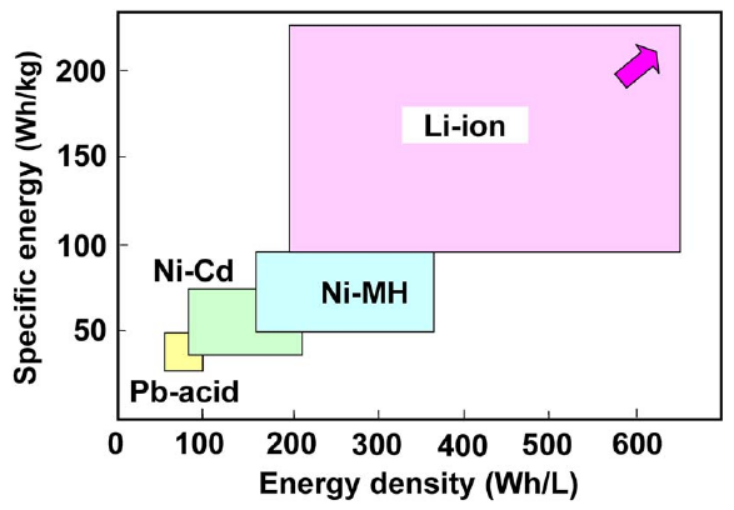
\includegraphics[width=0.6\textwidth]{comparisson-liion.png}
	\caption{Gr\'afica comparativa entre distintas tecnologías de baterías.}
	\label{comparisson_batt}
    \end{center}
\end{figure}

\noindent La aplicación práctica de las baterías de Litio-ion involucra la
integración de las mismas dentro de un sistema, involucrando un controlador
central (\acrshort{BMS}), sistemas de refrigeración, sensores y conectores entre
las celdas. En tales sistemas las celdas pueden conectarse de distintas formas,
por ejemplo, pueden conectarse en paralelo, para incrementar la capacidad del
pack, en serie, para incrementar el voltaje, o combinadas para lograr ambos
cometidos al mismo tiempo. Por ejemplo, un auto eléctrico de la marca
\emph{Tesla}, posee un pack de baterías de 85KWh compuesto por 7104 celdas, con
una arquitectura de 16 módulos conectados en serie , donde cada uno posee 444
celdas conectadas en paralelo.

%\newpage

\subsection{Modelado de bater\'ias de litio-ion}\label{litioModel}

\noindent Como se menciona anteriormente, las celdas de litio-ion son utilizadas
ampliamente en el mercado de consumo electr\'onico para un gran espectro de 
aplicaciones. Sin embargo, su fiabilidad y tiempo de vida son limitados y 
depende considerablemente de condiciones ambientales como también de su uso 
hist\'orico. Por lo tanto, se necesitan modelos de bater\'ias exactos y eficaces 
para que sean correctamente monitoreados por un \acrshort{BMS}.

\noindent Una celda, como se describe en la Secci\'on \ref{battery_fun}, puede 
ser caracterizada como un sistema electrotermoqu\'imico y actualmente existen 
una cantidad numerosa de modelos que logran describir el funcionamiento tanto 
est\'atico como din\'amico de la misma. Un modelo exacto y eficiente permite 
optimizar al m\'aximo el ciclo de vida de una bater\'ia ya que permite 
obtener informaci\'on sobre el \acrshort{SOC} como tambi\'en conocer 
par\'ametros cr\'iticos de la bater\'ia como por ejemplo, el perfil de descarga 
de la misma permitiendo ajustar los distintos algoritmos de protecci\'on y/o 
ecualizaci\'on que se apliquen en el desarrollo del \acrshort{BMS}.

A continuaci\'on se definen y se comparan los distintos modelos disponibles 
en la literatura actual. Esta comparaci\'on es basada en tres criterios:

\begin{description}
    \item [\textbf{Precisi\'on}:] La precisi\'on define cu\'an cercano un modelo
        puede predecir los valores de las variables de inter\'es de una
        bater\'ia.
    \item [\textbf{Complejidad}:] Se refiere a la cantidad de par\'ametros que
        necesita el modelo. Dependiendo de la complejidad del modelo, el 
        c\'alculo del mismo tomar\'a mayor o menor tiempo, cuestionando su 
        utilidad para una aplicaci\'on en tiempo real.
    \item [\textbf{Interpretaci\'on f\'isica}:] Esto se define como el nivel de
        interpretaci\'on anal\'itico que el modelo puede dar con respecto al
        funcionamiento interno de una bater\'ia.
\end{description}

\subsubsection{Modelos F\'isicos}\label{phyModel}

\noindent Los modelos f\'isicos, o tambi\'en conocidos como cajas blancas, son 
modelos de bajo nivel con un grado de exactitud muy alto. Permiten describir la 
estructura de los materiales y logran describir los complejos fen\'omenos 
electroqu\'imicos que suceden dentro de celda, tambi\'en denominados fen\'omenos 
termodin\'amicos, kin\'eticos y de transporte.

\noindent La bibliograf\'ia \cite{Schmidt2013} presenta un resumen del 
fen\'omeno f\'isico como se muestra en la Figura \ref{schmidt_fen_fis}. En ella, 
se pueden observar cuatro procesos en tres regiones de operaci\'on: las dos 
fases s\'olidas del material de los electrodos, y la fase l\'iquida del 
electrolito.

\begin{figure}[h!]
    \begin{center}
        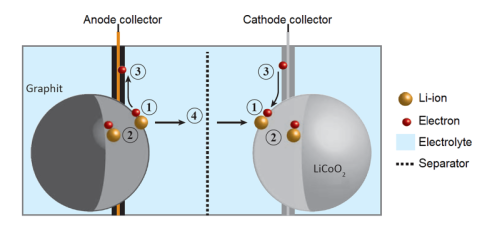
\includegraphics[width=0.7\textwidth]{schmidt_proceso_fisico.png}
        \caption{Descripci\'on gr\'afica del proceso interno de una celda de litio-ion.}
        \label{schmidt_fen_fis}
    \end{center}
\end{figure}

\noindent El primer proceso se denomina \emph{pasaje de cargas} y se da en 
la primer regi\'on de operaci\'on: la fase s\'olida del electrodo. 
Este proceso describe la intercalaci\'on como tambi\'en la desintercalaci\'on 
de los iones de litio dentro del material activo. El segundo proceso, ocurre 
en la misma regi\'on, y se la denomina la \emph{difusi\'on del estado s\'olido} 
de los iones de litio forzado por el gradiente de concentraci\'on de iones entre 
la superficie y el volumen del electrodo. El tercer proceso, se describe como 
la \emph{conducci\'on de electrones} entre un electrodo y otro a trav\'es de 
un circuito externo. Por \'ultimo, el cuarto proceso es la \emph{conducci\'on de 
iones} en el electrolito a trav\'es del separador, que tambi\'en es forzado for 
un gradiente de concentraci\'on y basado en la difusi\'on pero ocurre a mucha 
mayor velocidad que en los electrodos.

\noindent Estos tipos de modelos dependen de una gran cantidad de par\'ametros,
como tambi\'en de ecuaciones diferenciales interdependientes, para poder 
replicar el comportamiento de una celda se utilizan coeficientes de difusi\'on y 
propiedades de los materiales dentro de las ecuaciones dependientes del mismo. 
Los autores en \cite{Li2016} se basan en un modelo unidimensional a lo largo de 
la secci\'on de la celda, dividiéndolo en cinco secciones, aplicando las 
siguientes ecuaciones diferenciales: 

\begin{itemize}
    \item \textbf{Conservaci\'on de carga en un s\'olido homog\'eneo}
        \begin{equation}
            \nabla (-\sigma\nabla\upvarphi_s)=-j^{Li} 
            \label{Chrg_cons_hom_sol}
        \end{equation}	
    \item \textbf{Conservaci\'on de masa en un s\'olido homog\'eneo}
        \begin{equation}
            \frac{\partial c_s}{\partial t}=\nabla \cdot (D_s\nabla c_s) 
            \label{Mass_cons_hom_sol}
        \end{equation}	
    \item \textbf{Conservaci\'on de masa en un electrolito homog\'eneo}
        \begin{equation}
            \varepsilon_e\frac{\partial c_e}{\partial t} + \nabla \cdot
            (-D_e\nabla c_e) = \left(\frac{1-t_+^0}{F}\right)j^{Li}
            \label{Mass_cons_hom_electrolyte}
        \end{equation}	
    \item \textbf{Conservaci\'on de carga en un electrolito homog\'eneo}
        \begin{equation}
            \nabla \cdot (\upkappa \nabla \upvarphi_e + \upkappa_D \nabla \ln 
            c_e) = -j^{Li}
            \label{Chrg_cons_hom_electrolyte}
        \end{equation}	
    \item \textbf{Ecuaci\'on de Butler-Volmer:} Esta ecuaci\'on representa el
        movimiento de cargas en una uni\'on entre un s\'olido conductor y una
        soluci\'on de iones de litio con el efecto de doble capa
        \begin{equation}
            j^{Li} =
            a_si_0\left[{e^\frac{F\eta}{2RT}-e^{-\frac{F\eta}{2RT}}}\right] + 
            a_sC_{dl}\frac{\partial{(\upvarphi_s - \upvarphi_e)}}{\partial t}
            \label{Butler_Volmer_kinetics}
        \end{equation}	
\end{itemize}

En las ecuaciones \ref{Chrg_cons_hom_sol} - \ref{Butler_Volmer_kinetics}, se 
utilizan las siguientes variables:

\begin{description}
    \item [$\mathrm{\sigma}$]: Conductividad de la fase s\'olida del
        electrodo.
    \item [$\mathrm{\upvarphi_s}$]: Potencial el\'ectrico de la fase
        s\'olida.
    \item [$\mathrm{\upvarphi_e}$]: Potencial el\'ectrico del
        electrolito.
    \item [$\mathrm{j^{Li}}$]: Densidad de corriente producida por el
        consumo de iones de litio.
    \item [t]: Tiempo transcurrido.
    \item [c]: Concentraci\'on de iones de litio.
    \item [D]: Coeficiente de difusi\'on del material.
    \item [F]: Constante de Faraday.
    \item [$\mathrm{\varepsilon}$]: Fracci\'on por volumen.
    \item [$\mathrm{t_+^0}$]: N\'umero de transferencia.
    \item [$\mathrm{\upkappa}$]: Conductividad del electrolito.
    \item [$\mathrm{\upkappa_D}$]: Conductividad de la difusi\'on.
    \item [$\mathrm{i_0}$]: Corriente de intercambio.
    \item [$\mathrm{\eta}$]: Sobretensi\'on.
    \item [a]: \'Area espec\'ifica de la secci\'on.
    \item [$\mathrm{C_{dl}}$]: C\'apacidad de la doble capa.
\end{description}

A pesar de su alta exactitud, este tipo de modelo resulta complejo de
implementar en sistemas de tiempo real debido a la gran cantidad de ecuaciones
diferenciales a implementar con su extensa cantidad de par\'ametros a ajustar en
el mismo, imposibilitando su uso en veh\'iculos el\'ectricos.

\subsubsection{Modelos emp\'iricos}\label{empModels}

\noindent Los modelos emp\'iricos, tambi\'en conocidos como \emph{cajas negras},
son aquellos que describen a la batería en puntos de trabajo definidos y que
proveen pobres o incluso nulos conocimientos sobre el funcionamiento interno del
sistema, desconociéndose incluso el significado f\'isico de mucho de sus
par\'ametros internos del modelo. Las aproximaciones matem\'aticas que se
utilizan para definir la funci\'on transferencia entre las entradas y las
salidas de estos modelos permiten que los mismos sean f\'aciles de configurar
como tambi\'en generar predicciones y respuestas r\'apidas. Sin embargo, la
exactitud es limitada, especialmente si el modelo es muy simple, aunque puede
ser mejorado si se combina con un modelo de bajo nivel.

\subsubsection{Modelos abstractos}\label{absModels}

\noindent Tambi\'en conocidos como \emph{cajas grises}, los modelos abstractos 
proveen una representaci\'on alternativa de la entidad f\'isica a modelar. 
A pesar de que hay varias formas posibles de realizarlo, la m\'as utilizada 
dentro de la bibliograf\'ia es su representaci\'on en un circuito el\'ectrico 
equivalente. Los modelos basados en circuitos son simples y pr\'acticos porque 
permiten que el proceso electroqu\'imico que ocurre dentro de la celda sea 
reemplazado por un simple circuito. La correlaci\'on con las din\'amicas de la 
bater\'ia son preservados sin comprometer demasiada exactitud en su 
predicci\'on.

\noindent El costo de configuraci\'on para tales modelos es reducido en 
comparaci\'on a modelos de bajo nivel, sin embargo \'estos requiren de 
\emph{Look-up Tables} para coincidir con los datos experimentales. 
La complejidad de los mismos es m\'as flexible dependiendo de la unidad de 
c\'omputo como tambi\'en de la memoria disponible. Los mismo se pueden 
complejizar utilizando efectos de segundo \'orden, tales como la temperatura, 
degradaci\'on de la capacidad como tambi\'en el envejecimiento de las celdas.

\noindent A continuaci\'on se describen los modelos m\'as utilizados dentro de 
la literatura actual.

\subsubsubsection{Circuito simple}

\noindent El circuito el\'ectrico más simple que representa una bater\'ia de 
litio-ion es un circuito con constante de tiempo cero que se puede observar en 
la Figura \ref{zero_time_constant_sch}. Si el usuario no necesita representar la 
din\'amica de la bater\'ia, este modelo es capaz de representar el 
comportamiento est\'atico del sistema. 

\begin{figure}[h!]
    \begin{center}
        \begin{circuitikz}[american voltages]
            \draw 
                (0, 0) -- (3.5, 0)
                (0, 0) -- (0, .5)
                (0, 1.5) to[american voltage source, v_=$V_{OCV}$] (0, 0.5)
                (0, 1.5) -- (0, 2) to[R, l_=$R_S$] (3, 2) 
                to [short, i_=$I_{batt}$] (3.5, 2)
                (4, 2) to [open, v=$V_{batt}$] (4, 0);
        \end{circuitikz}
        \caption{Modelo de constante de tiempo cero para una celda de litio 
                 ion.}
        \label{zero_time_constant_sch}
    \end{center}
\end{figure}


\noindent El \acrshort{OCV} se relaciona directamente con el \acrshort{SOC},
definido en la Ecuación \ref{ocv_soc_ztc}

\begin{equation}
    SoC = \frac{C_{current}}{C_{full}}\dot 100\% \label{ocv_soc_ztc}
\end{equation}

\noindent Donde $\mathrm{C_{current}}$ es la cantidad de carga disponible en la 
celda y $\mathrm{C_{full}}$ es la capacidad de la celda cuando est\'a 
completamente cargada. La ecuaci\'on del modelo es expresada en la Ecuaci\'on 
\ref{vbatt_ocv_soc_ztc}.

\begin{equation}
    V_{batt} = V_{OC} - R_S \times I_{batt} \label{vbatt_ocv_soc_ztc}
\end{equation}

\noindent La curva del \acrshort{OCV} como funci\'on del tiempo muestra una 
caida del voltaje para ciertas condiciones de descarga. Los importantes 
par\'ametros que afectan el proceso de descarga son la corriente de descarga, 
la temperatura y la historia de carga/descarga.

\noindent El efecto de la temperatura en el proceso de descarga es visto a
temperaturas mucho más bajas que a temperatura ambiente, donde la actividad
qu\'imica disminuye y la resitencia de la bater\'ia aumenta. A temperaturas
m\'as altas que la ambiente, la resistencia interna disminuye, mejorando la
velocidad de la actividad qu\'imica, por lo tanto, y desafortunadamente,
induciendo un efecto de auto descarga.

\noindent La desventaja principal del modelo de constante de tiempo cero es que 
no contempla la din\'amica de las celdas. Sin embargo, esto puede ser mitigado 
de forma f\'acil agregando un tanque RC en serie a la resistencia (\emph{Fig.
\ref{one_time_constant_sch}}), que describe la respuesta din\'amica de la 
bater\'ia durante el proceso de carga/descarga.

\begin{figure}[h!]
    \begin{center}
        \begin{circuitikz}[american voltages]
            \draw 
                (0, 0) -- (7, 0)
                (0, 0) -- (0, 1)
                (0, 2) to[american voltage source, v_=$V_{OCV}$] (0, 1)
                (0, 2) -- (0, 3) to[R, l_=$R_s$] (3, 3) to[R, l_=$R_p$] (6, 3)
                (3, 3) to[short, *-] (3, 1.5) to [C, l_=$C_p$] 
                (6, 1.5) -- (6, 3) to [short, i_=$I_{batt}$] (7, 3)
                (7.5, 3) to [open, v=$V_{batt}$] (7.5, 0);
        \end{circuitikz}
        \caption{Modelo de primer \'orden para una celda de litio-ion.}
        \label{one_time_constant_sch}
    \end{center}
\end{figure}

\noindent La exactitud del modelo y su comportamiento din\'amico, pueden ser 
mejorados agregando m\'as tanques RC al circuito, esto a su vez incrementa la
complejidad del mismo. 

\subsubsubsection{Modelos basados en el espectro de impedancia}

La espectroscopía de impedancia electroquímica (\acrshort{EIS}, del ingl\'es
\acrlong{EIS}), es una técnica utilizada para describir las propiedades
eléctricas y dieléctricas de las celdas de ion-litio. También se la conoce como
Espectroscopía de Impedancia AC, debido a la que su implementación está
fundamentalmente basada en excitaciones de señales alternas.

La implementación de la EIS puede realizarse en modos distintos, excitando la
celda tanto con una señal de voltaje como con una señal de corriente.
Generalmente las señales de excitación son pequeñas señales sinusoidales, con lo
cual al excitar la celda por corriente podemos asegura la conservación del
estado de carga, ya que la integración en el largo plazo de la pequeña señal de
corriente es cero. Cuestion que no puede ser asegurada al ensayar la celda
exitada por tensión. La impedancia es calculada para señales de excitación con
diferentes frecuencias, que sean de interés en el espectro de análisis.

Para aplicar este m\'etodo, es necesario un sistema lineal invariante en el
tiempo. Por lo tanto, dado que las bater\'ias son sistemas altamente no lineales
durante el proceso de carga y descarga, el \acrshort{EIS} es aplicado a niveles
de \acrshort{SOC} donde la bater\'ia haya alcanzado un determinado estado de
relajación y reposo, para garantizar determinada linealidad necesaria.

\noindent La impedancia (Z) es una variable compleja representada en en el 
diagrama de Nyquist por una componente real y otra imaginaria. 
La Figura \ref{EIS_Nyquist} muestra un t\'ipico diagrama de Nyquist, 
como resultado de varias mediciones \acrshort{EIS} de una celda de litio-ion a
distintos niveles de \acrshort{SOC}. Cuantitativamente, los valores dependen de 
varios factores, como mencionamos anteriormente, la temperatura, 
el \acrshort{SOC} y la corriente de carga/descarga.

\begin{figure}[h!]
    \begin{center}
	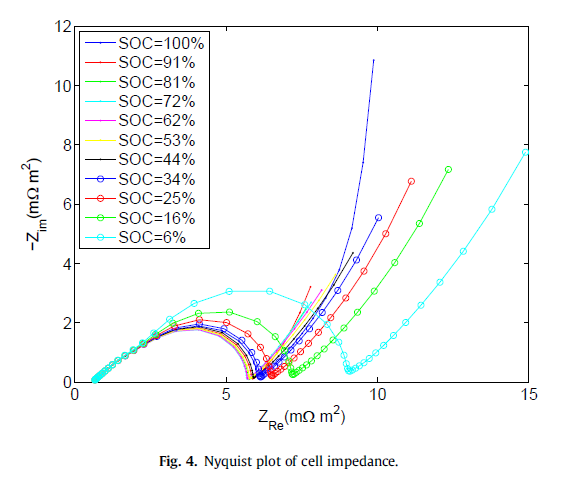
\includegraphics[width=0.4\textwidth]{EIS_Nyquist.png}
	\caption{Diagrama de Nyquist - Espectroscopía Dieléctrica (EIS) de 
	una batería de Li-Ion obtenida por barrido frecuencial.}
	\label{EIS_Nyquist}
    \end{center}
\end{figure}
\FloatBarrier

\noindent La curva puede ser subdividida seg\'un los rangos de frecuencia en
distintas secciones, como se puede observar en la Figura
\ref{EIS_nyquist_sections}. Estas secciones est\'an asociadas con fen\'omenos
f\'isicos y electroqu\'imicos bien definidos que ocurren dentro de la celda.

\noindent La secci\'on con $\mathrm{Z" < 0}$ consiste de tres \'areas bien
reconocibles. El arco a frecuencias muy bajas (cercanas a la corriente continua)
se asocia con el comportamiento de difusi\'on introducido en la Seccion
\ref{battery_fun} y es representado por la impedancia de \emph{estado s\'olido
de Warburg}. El segundo arco a frecuencias un poco m\'as altas (arco [ii] en
Fig.  \ref{EIS_nyquist_sections}) corresponde a la kin\'etica de la
transferencia de carga. El tercer y arco m\'as pequeño cerca del eje real (arco
[iii] en Fig.  \ref{EIS_nyquist_sections}) representa los efectos entre capas de
la interfaz s\'olida del electrolito.

\begin{figure}[h!]
    \begin{center}
	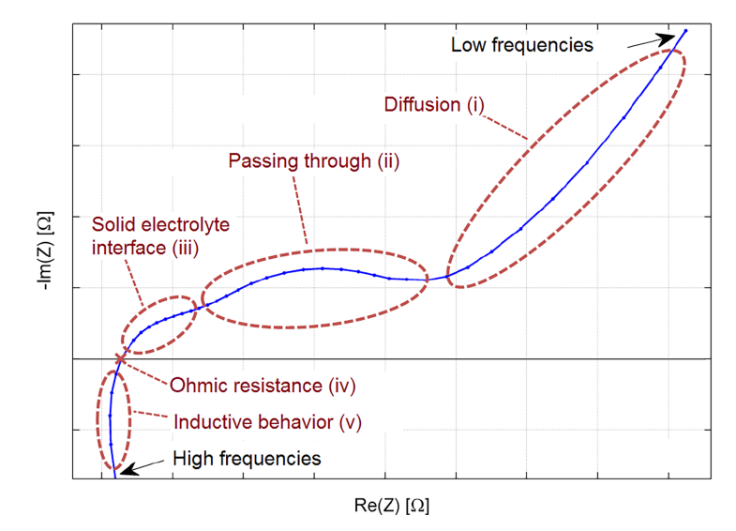
\includegraphics[width=0.7\textwidth]{EIS_nyquist_section.png}
	\caption{Secciones identificables dentro del diagrama de Nyquist.}
	\label{EIS_nyquist_sections}
    \end{center}
\end{figure}
\FloatBarrier

\noindent El punto (iv) de la Figura \ref{EIS_nyquist_sections} representa la 
resistencia \'ohmica total del sistema, incluyendo la resistencia del 
electrolito como tambi\'en la de los electrodos. Este punto generalmente occurre 
a una frecuencia dentro del rango de los KHz pero puede variar considerablemente 
con el diseño de la celda y los materiales utilizados.

\noindent Las altas frecuencias muestran un comportamiento inductivo con 
$\mathrm{Z" > 0}$ (secci\'on (v) de la Figura \ref{EIS_nyquist_sections}) 
correspondiente a la estructura porosa de los electrodos y los conectores de la 
bater\'ia.

\noindent El circuito equivalente de la respuesta de la impedancia es
introducido en \cite{Moss} y se puede observar en la Figura
\ref{sch_modelo_EIS}

\begin{figure}[h!]
    \begin{center}
        \begin{circuitikz}
            \draw
            (0, 0) to[L, o-, l=$L_s$] (2, 0) to [R, l=$R_s$] (4, 0) to[R,
            l=$R_{p1}$] (6, 0)
            (4, 0) to [short, *-] (4, -2) to [C, l=$C_{p1}$] (6, -2) to [short, -*]
            (6, 0) to[short, -*] (7, 0) to [C, l=$C_{dl}$] (11, 0)
            (7, 0) to[short] (7, -2) to[R, l=$R_{CT}$] 
            (9, -2) to[R, l=$Z(\omega)$] (11, -2) to[short, -*] (11, 0)
            to[C, -o, l=$C_{int}$] (12, 0);
        \end{circuitikz}
        \caption{Modelo equivalente a la respuesta del \acrshort{EIS}}
        \label{sch_modelo_EIS}
    \end{center}
\end{figure}
\FloatBarrier

\noindent Donde los componentes representan las siguientes partes f\'isica de 
la celda:

\begin{itemize}
    \item $\mathrm{C_{dl}}$: Capacitancia electroqu\'imica de doble capa
        de la celda.
    \item $\mathrm{R_{CT}}$: Resistencia a la corriente
        far\'adica
    \item $\mathrm{C_{int}}$: Capacitancia de intercalaci\'on
        correspondiente a la acumuluaci\'on de iones de litio dentro de la
        matriz del electrodo.
    \item $\mathrm{Z(\omega)}$: Impedancia de estado s\'olido de Warburg
        que depende de la frecuencia del ensayo.
\end{itemize}

\noindent En \cite{Moss} se sugiere la substituci\'on de la impedancia de 
difusi\'on de Warburg con una cadena de tanques RC. La nueva cadena no refleja 
la impedancia del elemento de Warburg pero representa una aproximaci\'on 
con una exactitud aceptable. Tomando esta aproximaci\'on en consideraci\'on, se 
valida el uso de modelos el\'ectricos para modelar celdas en un circuito 
compuesto por una fuente de tensi\'on con una resistencia $\mathrm{R_s}$ y una 
cadena de tanques RC conectadas en serie. Esto es solo posible gracias a las 
relaciones de Kramers-Kronig \cite{Schmidt2013}, que pueden ser aplicadas en 
redes equivalentes, y sugiere que distintos circuitos pueden tener una respuesta 
equivalente o similar sin tener la misma topolog\'ia. En otras palabras, la 
bater\'ia puede ser modelada con una topolog\'ia m\'as simple usando elementos 
que no tienen una directa interpretaci\'on f\'isica. Este modelo es v\'alido, 
porque tiene la misma respuesta en frecuencia, y es m\'as f\'acil de 
parametrizar.

\subsubsection{Comparaci\'on de modelos y su evaluaci\'on para aplicaciones
en veh\'iculos el\'ectricos}\label{compModels}

\noindent La Tabla \ref{table_comp_models} presenta una comparaci\'on de los
modelos seg\'un el criterio previamente explicado. Los modelos simples pueden
ser menos costosos desde un punto de vista computacional como tambi\'en en
desarrollo, a su vez, \'estos son más susceptibles a incertezas en los
par\'ametros del mismo. Por el otro lado, modelos complejos necesitan mayor
tiempo para resolver los algoritmos inherentes a ellos.  Dependiendo de la
aplicaci\'on, la extracci\'on del m\'etodo del modelo y usabilidad deben ser
evaluados antes de comenzar su desarrollo.  Dentro de un ambiente de
laboratorio, se puede invertir m\'as tiempo para extraer un modelo m\'as
preciso. Sin embargo, en el campo se necesitan resultados de forma r\'apida para
evaluar si las celdas son aptas para ser aplicadas en un veh\'iculo, por
ejemplo, en estos casos los modelos son utilizados para el desarrollo de un
\acrshort{BMS} como es lo que se busca en el presente trabajo. 

\noindent Tener una extensa comprensi\'on de la bater\'ia en estos casos no es
necesario, aunque puede resultar beneficioso. Dado que el mismo es embebido
dentro de una unidad de monitoreo en tiempo real, como puede ser un 
\acrshort{MCU} y/o \acrshort{FPGA}. Es m\'as conveniente que el modelo sea 
simple, para que los tiempos de c\'omputo no sean muy altos comprometiendo 
niveles aceptables de exactitud en los mismos. 

\begin{table}[h!]
\begin{center}
\begin{tabular}{@{}ccccc@{}}
\textbf{Modelos} & \textbf{Exactitud} & \textbf{Complejidad} &
\textbf{Interpretaci\'on f\'isica} & \textbf{Aplicaci\'on apropiada}\\
\hline
F\'isicos   & Muy alta  & \textgreater{}50 par\'ametros         & Alta
& diseño de de bater\'ias \\\hline Emp\'iricos & Media 
& 2 a 3 par\'ametros & Baja & Predicciones\\ 
\hline Abstractos & Media & 2 a 30 par\'ametros & Limitada & 
Monitoreo y diagn\'ostico
\end{tabular}
\caption{Resumen de la comparaci\'on entre modelos de celdas de litio-ion.}
\label{table_comp_models}
\end{center}
\end{table}

\subsection{Algoritmos de Estimaci\'on del Estado de Carga}\label{algSoc}

\noindent El \acrshort{SOC} es el equivalente a medir la cantidad de combustible
restante en un veh\'iculo convencional basado en combustibles f\'osiles. La
funci\'on principal de esta variable es comunicar de forma instintiva el estado
de la bater\'ia al conductor y, al mismo tiempo, evitar problemas tales como la
sobrecarga y sobredescarga del pack de bater\'ias, en otras palabras, mantener
el pack de bater\'ia dentro de la zona de operaci\'on segura como tambi\'en 
lograr mantener las celdas ecualizadas entre sí.

\noindent Esta tarea involucra el uso de sensores que permitan obtener las
señales de tensi\'on, corriente y temperatura de la bater\'ia para que el
circuito de control pueda procesarlos y computar el \acrshort{SOC},
usando uno de los algoritmos disponibles en la literatura actual que es
un tema en constante investigaci\'on debido al comportamiento no-lineal de las 
celdas de litio-ion inherentes a sus elementos electroqu\'imicos, que se ven 
afectados por condiciones internas y externas.

\noindent Cuando se menciona el \acrshort{SOC}, se refiere a la relaci\'on entre
la capacidad de corriente que queda en la bater\'ia con respecto a la capacidad
total bajo determinadas condiciones (temperatura, corriente de carga/descarga,
envejecimiento, entre otras), y su expresi\'on matem\'atica se puede observar en
la Ecuaci\'on \ref{eq_soc_int}

\begin{equation}
    SOC = \frac{Q_c}{Q}\times100\% 
    \label{eq_soc_int}
\end{equation}

\noindent Donde, desde el punto de vista de los veh\'iculos el\'ectricos,
$\mathrm{Q_c}$ es la energía residual de la bater\'ia en el momento que se
calcula, y su unidad es Ah (Ampere-hora); Q es la capacidad total de la
bater\'ia teniendo la misma unidad que $\mathrm{Q_c}$.

\noindent El hecho de que la bater\'ia dependa de varios factores, obliga a que
la Ecuaci\'on \ref{eq_soc_int} sea modificada, obteniendo la siguiente 
expresi\'on (\emph{eq. \ref{eq_soc_extended}}).

\begin{equation}
    SOC(t) = SOC(t_0) - \int_{t_0}^t \frac{\eta I}{C_n }d\tau
    \label{eq_soc_extended}
\end{equation}

\noindent En la Ecuaci\'on \ref{eq_soc_extended}, $\mathrm{C_n}$ es la 
capacidad nominal de la bater\'ia (en Ah), $\mathrm{\eta}$ es la eficiencia 
cul\'ombica de la celda e I es la corriente que circula sobre la celda en el 
intervalo de tiempo $[t_{0}, t]$.

\noindent Adem\'as del comportamiento de la celda, tambi\'en se debe modelar el
efecto de envejecimiento de la celda sobre el estado de carga, que puede ser
afectado por el ensamblado de la bater\'ia, temperatura, condiciones de
ventilaci\'on, corriente de auto-descarga, concentraci\'on de electrolitos, por
el otro lado, tambi\'en se lo relaciona con inconsistencias entre las distintas
celdas que componen el pack de bater\'ias, como por ejemplo, voltaje,
resistencia interna, capacidad y otros parf'ametros que afectan el 
envejecimiento del pack. La relaci\'on del envejecimiento y el \acrshort{SOC} se
ve reflejado por el \acrshort{SOH}, que es una variable que permite cuantificar
la antigüedad de una bater\'ia. La influencia del envejecimiento de la celda
sobre el \acrshort{SOC} se puede expresar en la Ecuaci\'on \ref{soc_soh}.

\begin{equation}
    SOC(t) = SOH(t) - DOD(t) \label{soc_soh}
\end{equation}

\noindent En la Ecuaci\'on \ref{soc_soh}, SOH(t) es el estado de salud. 
Cuando la bater\'ia es nueva, se considera que el SOH est\'a a un 100\%. 
Por el otro lado, el \acrshort{DOD} (del ingl\'es, \acrlong{DOD}) indica cuanto 
de la capacidad total de la bater\'ia puede ser descargado realmente, este valor 
se toma en cuenta cuando solo se puede descargar el 80\% de la capacidad total 
de la celda.

\noindent Basado en caracter\'isticas experimentales y te\'oricas, existen 
varios m\'etodos para estimar el \acrshort{SOC} y pueden ser clasificados dentro 
de tres grupos: Los m\'etodos tradicionales de estimaci\'on que se basan 
meramente en datos experimentales, m\'etodos modernos basados en teor\'ias de 
control y, por \'ultimo, m\'etodos basados novedosos basados en algoritmos
pertenecientes a lo que hoy se denomina la \emph{ciencia de datos}.

\subsubsection{M\'etodos tradicionales basados en experimentos}
\label{tradSocMeth}

Estos m\'etodos dependen exclusivamente de una interpretaci\'on de mediciones
directas e indirectas de la bater\'ia, como por ejemplo, la corriente, 
la tensi\'on, la temperatura e, inclusive, el c\'alculo de otras variables en
base a estos valores con respecto al \acrshort{SOC}, por lo general se
caracterizan por ser simples de implementar mostrando un alto grado de error del
modelo. 

\subsubsubsection{M\'etodo en base al voltaje de circuito abierto}
\label{ocv_section}

\noindent La medici\'on del voltaje de circuito abierto, u \acrshort{OCV} (del
ingl\'es \acrlong{OCV}), se basa en la relaci\'on entre la medici\'on de este 
voltaje y el \acrshort{SOC} representado en la Ecuaci\'on \ref{ocv_soc_eq}.

\begin{equation}
    V_{OC} = f(SOC) \label{ocv_soc_eq}
\end{equation}

\noindent Esta relaci\'on se determina realizando el experimento \acrshort{HPPC} 
(del ingl\'es, \acrlong{HPPC}) que consiste en descargar la bater\'ia con pulsos 
de corrientes equivalentes a un tercio de su capacidad comenzando desde el 
100\% de la bater\'ia hasta un 10\% de su capacidad en donde, despu\'es de cada 
pulso, se deja descansar a la celda por un un intervalo de 2 horas, permitiendo 
que la misma se equilibre de forma t\'ermica y electroqu\'imica antes de aplicar 
el pr\'oximo pulso de corriente. Durante el proceso de este ensayo, se toman 
mediciones de corriente y tensi\'on en bornes de la bater\'ia, permiti\'endo 
obtener una curva de \acrshort{OCV} vs \acrshort{SOC} como se puede observar en 
la Figura \ref{soc_ocv_paper}.

\begin{figure}[h!]
    \begin{center}
        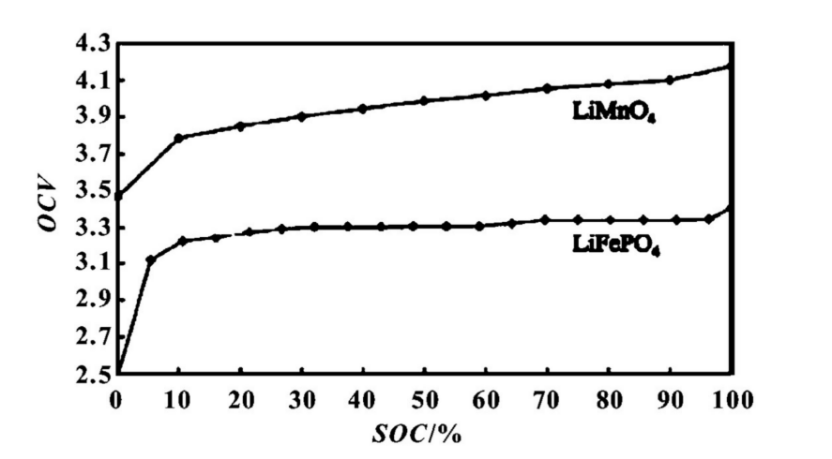
\includegraphics[width=0.6\textwidth]{soc_ocv_paper.png}
        \caption{Curva \acrshort{OCV} vs \acrshort{SOC} de una celda de hierro
        litio fosfato y otra de litio \'acido manganeso.}
        \label{soc_ocv_paper}
    \end{center}
\end{figure}

\noindent La ventaja del m\'etodo basado en la medici\'on del \acrshort{OCV} es
que es muy simple de implementar, solo hace falta tener una lectura de la
tensi\'on en bornes de la celda. Sin embargo, a pesar de su simpleza, el
m\'etodo no es apto para realizar una estimaci\'on en tiempo real debido a las
din\'amicas internas de la celda.

\noindent Por ejemplo, el voltaje de la celda tiene una respuesta muy din\'amica
ante fluctuaciones de corriente, como se puede observar en la Figura
\ref{relaxation_ocv}, lo que imposibilita utilizar este m\'etodo como estimador
del \acrshort{SOC} en tiempo real, ya que ante una pequeña circulaci\'on de
corriente la correlaci\'on entre el voltaje y el \acrshort{SOC} no es directa.

\begin{figure}[h!]
    \begin{center}
        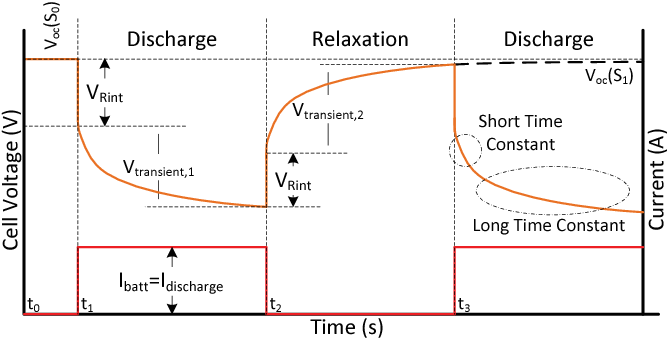
\includegraphics[width=0.7\textwidth]{ocv_relaxation.png}
        \caption{Repuesta de la tensi\'on de salida de una celda de Litio-ion
        ante un escal\'on de corriente}
        \label{relaxation_ocv}
    \end{center}
\end{figure}

\noindent Por el otro lado, las celdas de litio-ion poseen un voltaje de
hist\'eresis en el proceso de carga y descarga, como se puede observar en la
Figura \ref{histeresis_plot}, donde en la misma se muestrea el \acrshort{SOC}
para distintos per\'iodos de relajaci\'on, en ella se puede notar como
afecta el per\'iodo de relajaci\'on para realizar la estimaci\'on, donde a
mayor tiempo mejor es la estimaci\'on, esto se relaciona de forma directa con el
proceso de difusi\'on del litio dentro de la celda.

\begin{figure}[h!]
    \begin{center}
        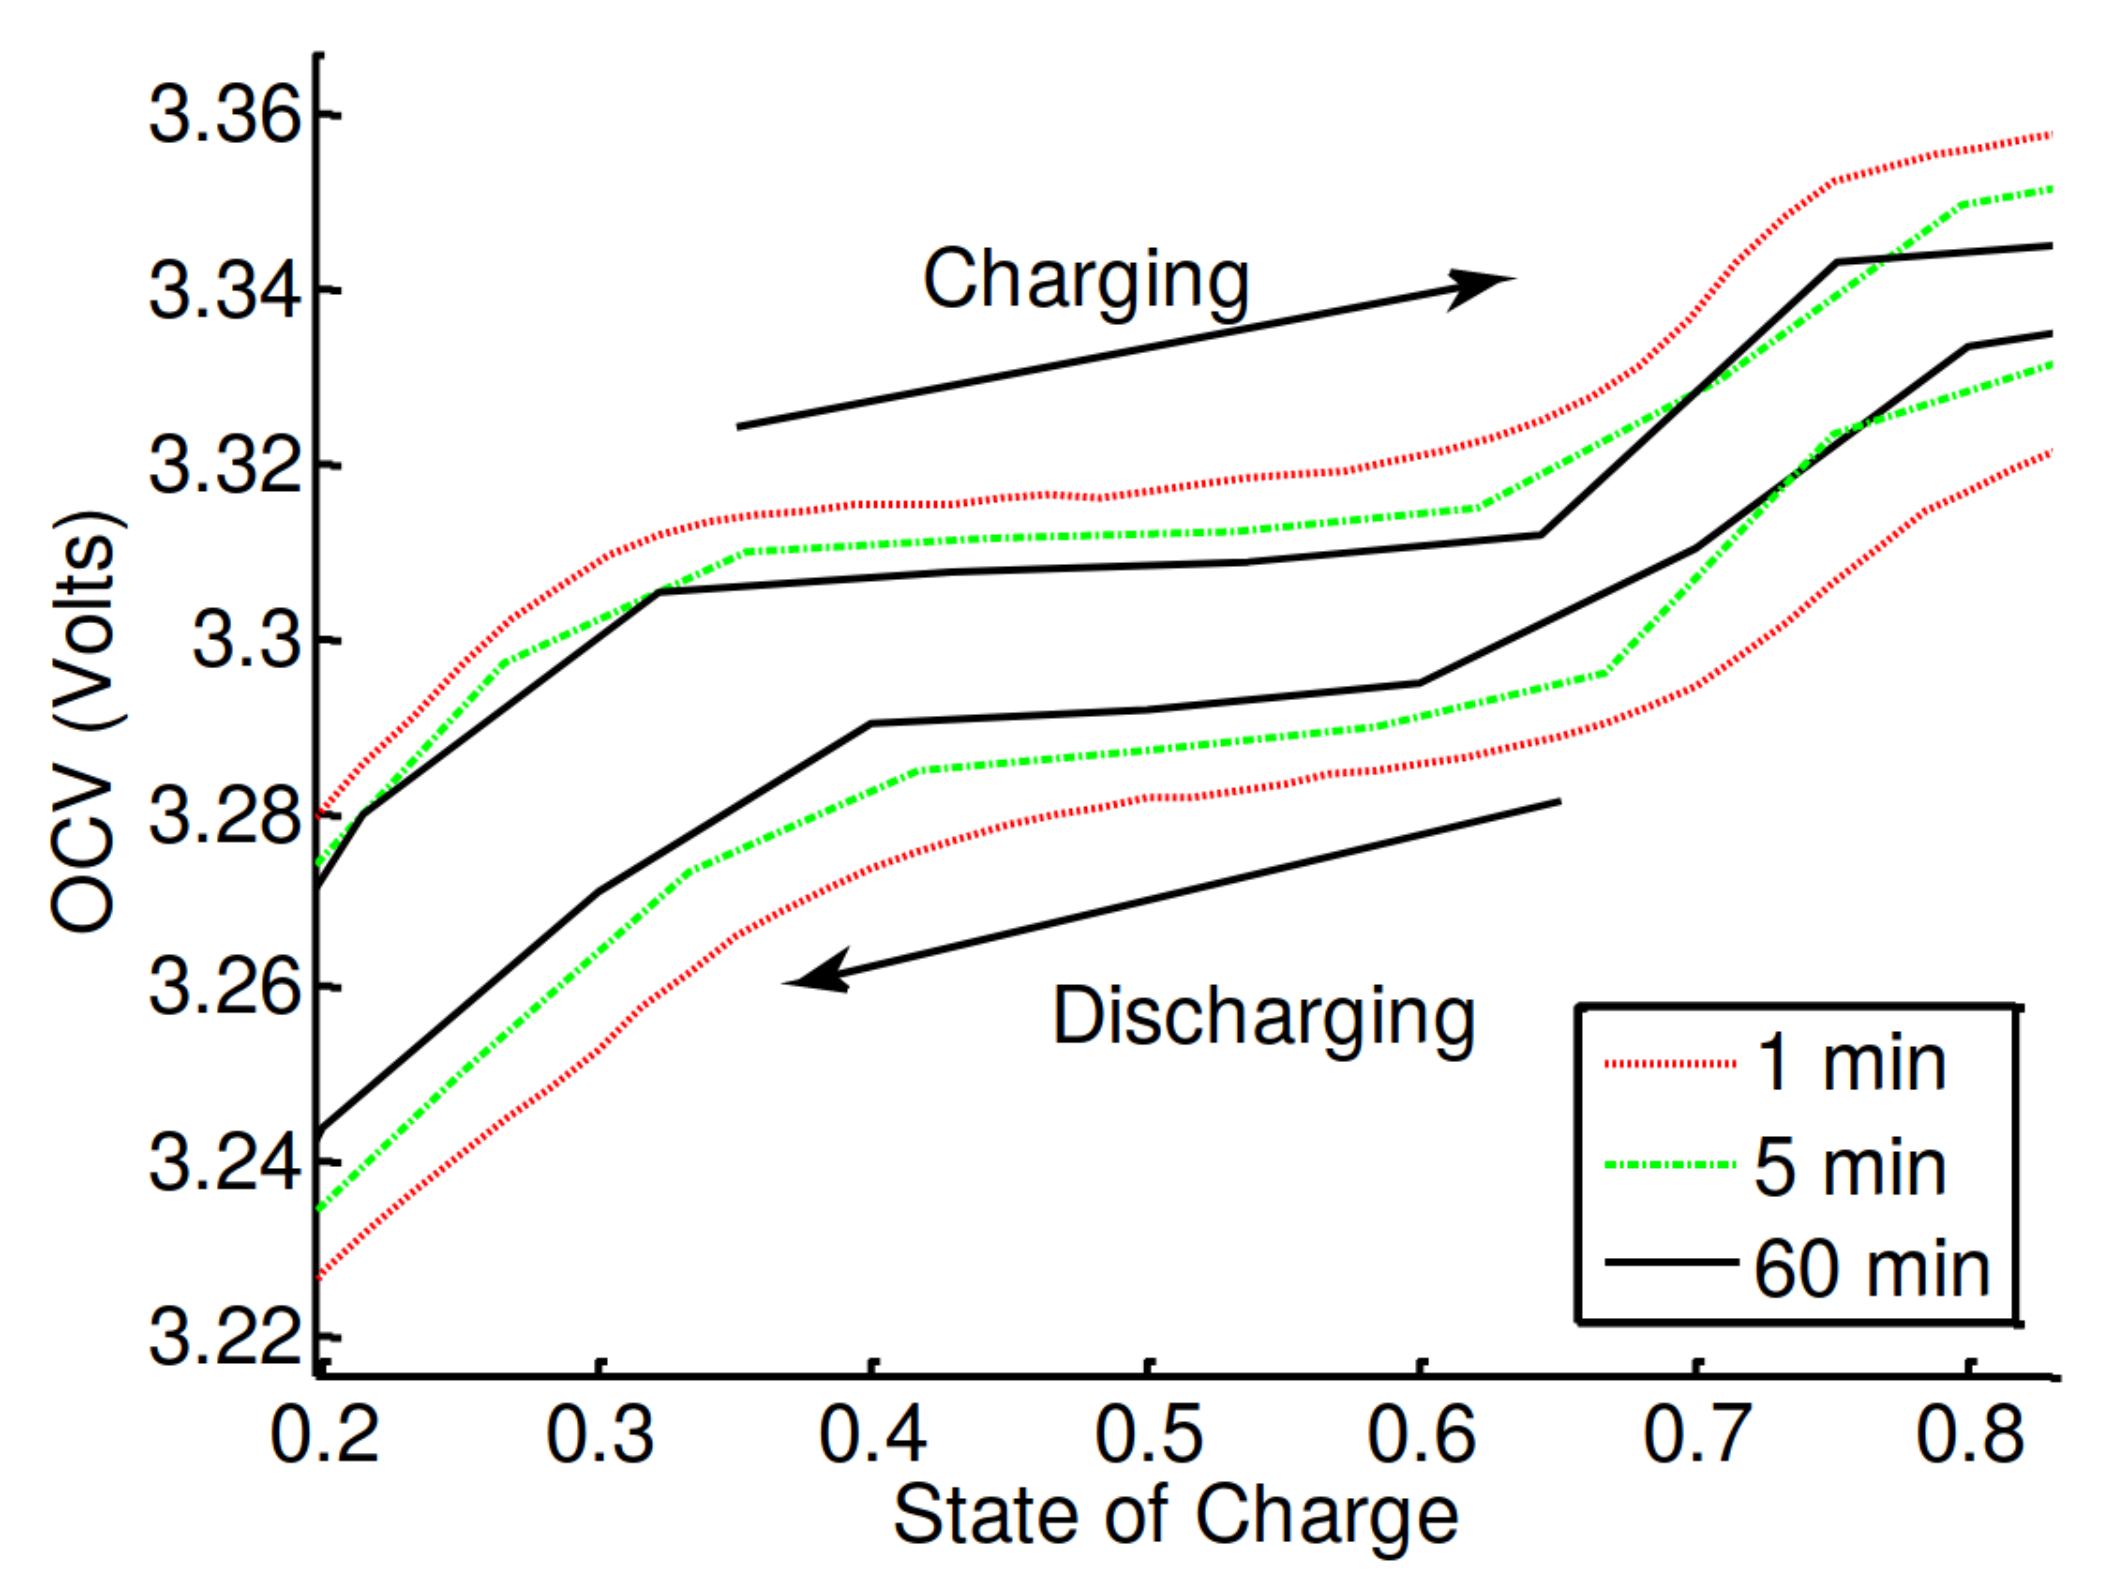
\includegraphics[width=0.5\textwidth]{soc_histeresis.png}
        \caption{curva \acrshort{OCV} vs \acrshort{SOC} durante el proceso de
            carga y descarga para distintos tiempos de relajaci\'on, denotando
            el fen\'omeno de hist\'eresis.} 
        \label{histeresis_plot}
    \end{center}
\end{figure}

\noindent Finalmente, la curva \acrshort{OCV} vs \acrshort{SOC} de la Figura
\ref{soc_ocv_paper} muestra secciones en la que la señal del \acrshort{OCV} es
plana ante una variaci\'on del \acrshort{SOC}, particularmente entre el 40\% y
el 60\%. Adem\'as, hay una variaci\'on muy pequeña en tensi\'on entre el 20\% y
80\%, lo cual, ante un m\'inimo error en la lectura de la tensi\'on de la celda
puede llevar a mediciones muy inexactas del \acrshort{SOC}. Estas observaciones
son los principales retos de estimar el \acrshort{SOC} utilizando solamente la
medici\'on del \acrshort{OCV}, lo cual llev\'o al desarrollo de nuevas
metodolog\'ias de estimaci\'on.

\newpage

\subsubsubsection{M\'etodo de integraci\'on de corriente}\label{ahMethod}

\noindent \'Este m\'etodo se basa en el c\'alculo de la circulaci\'on de 
corriente acumulada durante el proceso de carga y descarga de una bater\'ia. En 
la literatura se plantean varias versiones de la ecuaci\'on matem\'atica
utilizada por este m\'etodo, la m\'as utilizada se puede describir en la 
Ecuaci\'on \ref{ah_soc_general}.

\begin{equation}
    SOC = \frac{Q_0 + \int_{0}^t i_c\eta dt - \int_{0}^t i_d dt - S}{Q}
    \label{ah_soc_general}
\end{equation}

\noindent En la Ecuaci\'on \ref{ah_soc_general}, Q es la capacidad total de la 
bater\'ia, $\mathrm{Q_0}$ es la carga inicial de la celda, $\mathrm{\eta}$ es la 
eficiencia de carga, S es la cantidad estimada de auto-descarga de la celda, 
$\mathrm{i_c}$ es la corriente de carga e $\mathrm{i_d}$ es la corriente de 
descarga.

\noindent Por el otro lado, en \cite{ZHANG201524} tambi\'en se encuentran 
versiones mejoradas de \'este m\'etodo para corregir el error estimado. 
El principio de operaci\'on se puede observar en la Ecuaci\'on 
\ref{ah_soc_enhanced}.

\begin{equation}
    SOC = \alpha SOC_0 - \frac{1}{\delta c}\int \eta_\epsilon I dt
    \label{ah_soc_enhanced}
\end{equation}

En esta ecuaci\'on, $\mathrm{SOC_0}$ es obtenida por el m\'etodo de
\acrshort{OCV} descripto en la Secci\'on \ref{ocv_section}, $\mathrm{\alpha}$ es
el coeficiente que representa el factor de correcci\'on de auto-descarga y
envejecimiento de la celda, que se obtiene en base a varios experimentos en la
celda, $\mathrm{\delta}$ es el factor de correcci\'on por la capacidad de la
bater\'ia que se puede obtener a partir de la Ecuaci\'on
\ref{batt_cap_correction}. El par\'ametro $\mathrm{\eta_\epsilon}$ es la
eficiencia cul\'ombica equivalente de la celda, cuyo valor se obtiene unificando
la eficiencia cul\'ombica de distintas corrientes.

\begin{equation}
    \delta = 0.0010N^2 - 0.032N + 11.8819\label{batt_cap_correction}\;
    \text{donde N es el n\'umero de ciclos}
\end{equation}

\noindent El m\'etodo de integraci\'on de corriente tiene la ventaja de ser un
c\'alculo simple, estable y permite ser implementado en tiempo real.
Considerando la auto-descarga, temperatura, eficiencia de carga y descarga, el
m\'etodo puede alcanzar niveles de exactitud aceptables para una
implementaci\'on r\'apida en la estimaci\'on del \acrshort{SOC} en un BMS. Sin
embargo, este m\'etodo tiene dos principales desventajas:

\begin{enumerate}
    \item Dado que solo se integra corriente en un largo per\'iodo de tiempo, el
        m\'etodo es propenso a acumular considerable error en el tiempo.
    \item El mismo no logra eliminar la p\'erdida de la capacidad de carga como
        consecuencia del envejecimiento de la celda.
\end{enumerate}

\noindent Por esto mismo, varias bibliograf\'ias proponen fusionar el m\'etodo
por \acrshort{OCV} junto a \'este para compensar los errores inherentes, as\'i
obteniendo una metodolog\'ia simple y eficiente para estimar el \acrshort{SOC}
de una celda.

\subsubsubsection{Medici\'on de resistencia interna}\label{internalRMethod}

\noindent Este m\'etodo tiene el objetivo de relacionar la resistencia interna
de una celda con el \acrshort{SOC}, considerando la corriente de descarga y la
resistencia interna de la bater\'ia. Sin embargo, en la pr\'actica, la
relaci\'on entre los par\'ametros de una celda y el \acrshort{SOC} es bastante
compleja. En la etapa inicial y final de la descarga, la resistencia interna
aumenta considerablemente obteniendo como resultado grandes fluctuaciones,
mientras que durante el resto del proceso de descarga la resistencia interna se
caracteriza por una meseta, debido a ello, \'este m\'etodo es generalmente
implementado durante el principio y el final del proceso de descarga. Este 
comportamiento se puede observar en la Figura \ref{res_int_graph}.

\begin{figure}[h]
    \begin{center}
	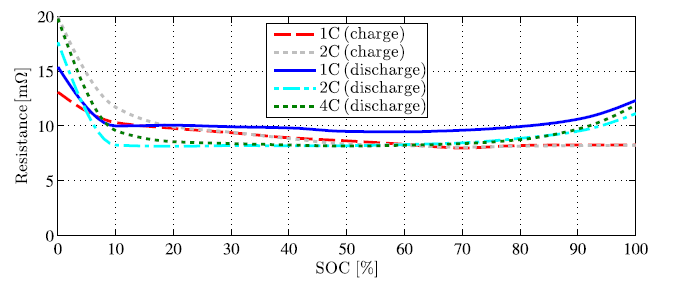
\includegraphics[width=0.7\textwidth]{Ro_vs_SOC.png}
	\caption{Resistencia en corriente continua de una batería de litio-ion vs. 
        SOC obtenida por HPPC}
	\label{res_int_graph}
    \end{center}
\end{figure}

\noindent La resistencia interna de una bater\'ia puede ser dividida en la
resistencia de corriente alterna y corriente continua. Por lo tanto,
\'este m\'etodo puede ser dividido en dos m\'etodos para cada una. 
La impendancia en alterna es la funci\'on transferencia entre el
voltaje y la corriente de la celda cuando se le aplica una corriente
alterna y ambos pueden ser medidos f\'acilmente con un medidor de impedancias. 
Sin embargo, a pesar de ser un m\'etodo muy simple de implementar, la relaci\'on 
de la resistencia interna con el SOC se acomplejiza dependiendo de la 
tecnolog\'ia de la bater\'ia, especialmente en las celdas de litio-ion.

\noindent El m\'etodo consiste en excitar la bater\'ia por breves instantes 
(menores a 10ms) con un pulso de corriente, asumiendo que este per\'iodo es lo 
suficientemente acotado para que la variaci\'on de tensi\'on sea atribuida a la 
resistencia interna y no a la carga/descarga de la bater\'ia, el c\'alculo de la 
resistencia se podr\'ia obtener seg\'un la Ecuaci\'on
\ref{rint_batt_eq}:

\begin{equation}
    \frac{\Delta V}{\Delta I} = R_{\ohm} \label{rint_batt_eq}
\end{equation}

Sin embargo, a pesar de su simpleza, este m\'etodo no resulta atractivo para
implementar en sistemas en tiempo real dado que, como se menciona anteriormente,
tiene una gran exactitud \'unicamente en bajos y altos valores de \acrshort{SOC},
adem\'as, tambi\'en debe inyectarse una corriente de valor conocido para poder
estimar su valor, resultando en mayor complejidad al circuito del
\acrshort{BMS}, dado que debe generar esta corriente constante de forma
peri\'odica y en tiempo real.

\noindent En resumen, los m\'etodos de estimaci\'on del \acrshort{SOC} basados
en experimentos, como se menciona anteriormente, tienen la ventaja de ser 
simples y f\'aciles de implementar, pero requieren de mucha inversi\'on 
experimental en las celdas en relaci\'on al bajo rendimiento que proveen en 
estimar de forma exacta el \acrshort{SOC}. Con respecto a la exactitud de 
estimaci\'on y caracter\'isticas de los ensayos de cada m\'etodo, se puede decir 
que:

\begin{itemize}
    \item \textbf{Estimaci\'on por OCV:} La exactitud de este m\'etodo depende
        exclusivamente del tiempo en el que la bater\'ia estuvo relajada,
        mientras mayor sea este tiempo m\'as exacto es la estimaci\'on.
    \item \textbf{Estimaci\'on por integraci\'on de corriente:} Es
        principalmente utilizado para determinar el \acrshort{SOC} inicial, pero
        su exactitud disminuye con el tiempo de medici\'on, debido a que la
        resistencia interna cambia constantemente y es propenso a acumular
        errores.
    \item \textbf{M\'etodo de resistencia interna:} \'Este m\'etodo es solo
        estable sobre la etapa final e inicial de descarga y tiene un alto grado 
        de precisi\'on, pero el tiempo de ensayo no se puede obtener de forma
        precisa por lo que genera un error en el mismo.
\end{itemize}


\subsubsection{M\'etodos modernos basados en la teor\'ia de control}
\label{controlTheoryMethod}

\noindent Dentro de la ingenier\'ia y las matem\'aticas, la teor\'ia de control
se encarga de modelar y controlar la din\'amica de un sistema,
independientemente de su naturaleza. Cuando una o m\'as variables de salida
necesitan seguir determinada referencia, un controlador manipula las entradas
del mismo para que el sistema pueda lograr el efecto deseado a su salida.

\noindent La mayor\'ia de los conceptos de la teoría de control modena
encuentran su fundamento en la posibilidad de medir las variables de interes del
sistema, de forma directa o indirecta, a partir de sensores y trasductores
eléctricos. Desafortunadamente, tal suposici\'on no siempre es v\'alida. Los
sensores f\'isicos siempre tienen limitaciones que afectan estos sistemas. Por
ejemplo, en algunos casos los sensores son componentes muy costosos tanto
econ\'omicamente como en su implementaci\'on, en otros casos la variable a medir
no puede ser accesible o f\'isicamente medible debido a ambientes hostiles.
Finalmente, los sensores inducen errores significativos, tales como el ruido,
retardo de fase, errores determin\'isticos y respuesta limitada en ancho de
banda.

\noindent Para mitigar este problema, se plantea el uso de \emph{observadores}. 
Los observadores son algoritmos que combinan señales que provienen de sensores 
con conocimientos del sistema para producir señales \emph{observadas}. 
\'Estas señales pueden ser igual de exactas que el sensado, menos costosas de 
producir, y de mayor confianza que las señales proveniente de sensores. 
Los observadores ofrecen al diseñador la alternativa de agregar nuevos 
sensores, o mejorar los existentes agregando solamente costo computacional, sin 
reimplementaciones de hardware ahorrando traer altos costos de diseño durante la
etapa de desarrollo de un producto.

\noindent El principio de operaci\'on de un observador se basa en combinar la
medici\'on de salida de la planta con conocimientos previos de los distintos 
componentes que modelan a la misma, obteniendo un mayor conocimiento sobre el 
comportamiento de la planta a comparaci\'on de utilizar solamente la señal de 
salida de la misma. Como se puede observar en la Figura \ref{role_observer}, el 
observador aumenta la capacidad del sensor de salida y provee una señal de 
realimentaci\'on a las leyes de control.

\begin{figure}[h!]
    \begin{center}
    \begin{tikzpicture}
        \draw (-.75, 0) node {Set Point};
        \draw[-stealth] (0, 0) -> (1, 0);
        \draw (1.5, 0) circle (0.5);
        \draw[-stealth] (2, 0) -> (2.5, 0);
        \draw (2.5, .5) rectangle (5, -.5) node[pos=.5]{Ley de Control};
        \draw[-stealth] (5, 0) -> (5.5, 0);
        \draw (6, 0) circle (0.5);
        \draw[-stealth] (6, 1) -> (6, 0.5);
        \draw (6, 1.5) node {Ruido};
        \draw[-stealth] (6.5, 0) -> (7, 0); 
        \draw (7, .5) rectangle (8.5, -.5) node[pos=.5]{Planta};
        \draw[-stealth] (8.5, 0) -> (9, 0);
        \draw (9, .5) rectangle (10.5, -.5) node[pos=.5]{Sensor};
        \draw (10.5, 0) -> (11, 0) -> (11, -4);
        \draw[-stealth] (11, -4) -- (9, -4);
        \draw (11, -4.5) node {Medici\'on de salida};
        \draw (9, -3.5) rectangle (4, -4.5) node[pos=.5]{Observador};
        \draw[-stealth](6.5, -2.5) -- (6.5, -3.5);
        \draw (6.5, -2) node {Modelo de la planta};
        \draw (4, -4) -- (1.5, -4);
        \draw (1.5, -4.5) node {Realimentaci\'on del observador};
        \draw[-stealth] (1.5, -4) -- (1.5, -.5);
    \end{tikzpicture}
    \caption{Rol del observador en un sistema de control}
    \label{role_observer}
    \end{center}
\end{figure}
\FloatBarrier

\noindent Sin embargo, la tecnolog\'ia del observador no necesariamente es la
soluci\'on final a estos problemas. Como mencionamos anteriormente, los
observadores agregan trabajo computacional al producto final y, adem\'as, la
robustes de los mismos, en comparación con un sensor equivalente, depende pura y
exclusivamente de la complejidad matemática del observador, especialmente cuando
la planta sufre modificaciones substancialles al evolucionar alrededor del punto
de operaci\'on. 

\noindent Dentro de los observadores disponibles, la bibliograf\'ia relacionada
a la estimaci\'on del \acrshort{SOC} hace un gran \'enfasis en la utilizaci\'on
del \emph{filtro de Kalman} como un buen candidato (\cite{spagnol_kalman}, 
\cite{zhihao_kalman} y \cite{atsushi_kalman}) obteniendo resultados
prometedores. A continuaci\'on se desarrolla su principio de funcionamiento, 
beneficios y como se utiliza como observador del \acrshort{SOC}.

\subsubsubsection{M\'etodo del Filtro de Kalman}\label{KalmanFilterMethod}

\noindent Dentro de las herramientas matem\'aticas que pueden ser utilizadas 
para estimaci\'on de variables a partir de mediciones ruidosas, una de las m\'as
conocidas y usadas es el \emph{Filtro de Kalman} \cite{kalman_filter_paper}. 
Esencialmente, el filtro de Kalman es un conjunto de ecuaciones matem\'aticas 
que implementan un estimador de tipo \emph{predictor-corrector} que es \'optimo 
en el sentido de que minimiza la covarianza del error dadas determinadas 
condiciones y, a pesar de que estas condiciones son rara vez dadas, se obtienen 
buenos resultados para varias aplicaciones.

\noindent En principio, el filtro logra estimar la variable de inter\'es usando 
un control de retroalimentaci\'on: El filtro estima el estado del proceso en 
determinado instante de tiempo y despu\'es obtiene la realimentaci\'on en forma 
de mediciones ruidosas, en base a esta realimentaci\'on, calcula el error y
reacomoda su ganancia para disminuir el mismo. Las ecuaciones del filtro se
dividen en dos grupos: \emph{ecuaciones de actualizaci\'on en el tiempo} 
y \emph{ecuaciones de actualizaci\'on de medici\'on}. El primer conjunto de
ecuaciones es responsable de proyectar la estimaci\'on el estado actual y la
covarianza del error en el tiempo, para obtener estimaciones \emph{a priori}. 
El segundo conjunto de ecuaciones son responsables de la realimentaci\'on, por 
ejemplo, incorporando nuevas mediciones dentro del estado estimado de forma 
\emph{a priori} para obtener una estimaci\'on \emph{a posteriori} mejorada.

\noindent Las ecuaciones de actualizaci\'on del tiempo tambi\'en pueden ser 
interpretadas como ecuaciones de \emph{predicci\'on}, mientras que las 
ecuaciores de actualizaci\'on de medici\'on pueden ser interpretadas como 
ecuaciones de \emph{correcci\'on}. Obteniendo como resultado, un algoritmo 
recursivo de tipo \emph{predictor-corrector} para resolver problemas num\'ericos 
como se puede observar en la Figura \ref{kalman_filter_sch}.

\begin{figure}[h!]
    \begin{center}
    \begin{tikzpicture}
        \draw (0, 0) node {Predicci\'on};
        \draw[-stealth] (0, -.25) to[out=-90, in=-90] (3, -.25);
        \draw (3, 0) node {Correcci\'on};
        \draw[stealth-] (0, .25) to[out=90, in=90] (3, .25);
    \end{tikzpicture}
    \caption{El ciclo perpetuo del filtro de Kalman. }
    \label{kalman_filter_sch}
    \end{center}
\end{figure}
\FloatBarrier

La actualizaci\'on en el tiempo proyecta el estado actual. Mientras que la
actualizaci\'on de medici\'on ajusta la proyecci\'on estimada previamente a una
actual medici\'on a ese instante.

Las ecuaciones específicas para la estimaci\'on del estado (o actualizaci\'on en
el tiempo) se representan en las Ecuaciones \ref{est_state} y \ref{est_uncert}.

\begin{align}
    \hat{x}_{n+1, n} &= F\hat{x}_{n,n} + Gu_n & & \textrm{Estimaci\'on de estado}
    \label{est_state} \\
    P_{n+1,n} &= FP_{n,n}F^T + Q & & \textrm{Estimaci\'on de incerteza}
    \label{est_uncert}
\end{align}

\noindent Donde F es una matriz (n x n, donde n es la cantidad de estados del 
sistema) que relaciona la proyecci\'on del estado con el estado actual, G es una 
matriz (n x l, donde l es la cantidad de entradas del sistema) que relaciona las 
señales de entrada con la proyecci\'on del estado del sistema y, por \'ultimo, 
Q (n x n) es la covarianza del ruido relacionado al proceso interno del sistema.

\noindent En las ecuaciones anteriores se puede observar como se proyecta el 
estado y la covarianza desde el paso n al paso n+1, obteniendo una predicci\'on 
del estado del sistema.

\noindent Por el otro lado, las ecuaciones relacionadas a la actualizaci\'on de 
las mediciones se pueden observar en las Ecuaciones \ref{kalman_gain},
\ref{estimate_w_measurement} y \ref{estimate_uncertainty}.

\begin{align}
    K_n &= P_{n, n-1}H^T(HP_{n,n-1}H^T + R_n)^{-1} & & \textrm{Ganacia de Kalman}
    \label{kalman_gain}\\
    \hat{x}_{n, n} &= \hat{x}_{n,n-1} + K_n \left(z_n - H\hat{x}_{n, n-1}\right) & & \textrm{Actualizaci\'on del estado}
    \label{estimate_w_measurement}\\
    P_{n, n} &= \left(I - K_nH\right)P_{n,n-1}\left(I - K_nH\right)^T + K_n R_{n} K_n^T & & \textrm{Actualizaci\'on de la covarianza}
    \label{estimate_uncertainty}
\end{align}
\FloatBarrier

\noindent Donde H es una matriz (z x n, donde z es la cantidad de mediciones y n
es la cantidad de estados del sistema) que indica la relación entre las
mediciones y el vector de estado al momento n, en el supuesto ideal de que no
hubiera ruido en las mediciones. y R es una matriz (z x z, donde z es la
candidad de mediciones) de covarianza del ruido de las mediciones (depende de la
resolución de los sensores utilizados).

\noindent La primer tarea durante el proceso de \emph{correcci\'on} es calcular 
la ganancia de Kalman, $\mathrm{K_k}$, despu\'es el algoritmo procede a medir el
proceso obteniendo la variable $\mathrm{z_k}$, y con esta informaci\'on generar
el estado \emph{a posteriori} incorporando las mediciones como se puede observar
en la Ecuaci\'on \ref{estimate_w_measurement}, que es similar a la Ecuaci\'on
\ref{est_state} pero con mediciones actuales utilizando la ganancia de Kalman
como un corrector. Por \'ultimo se obtiene una estimaci\'on del error de
covarianza \emph{a posteriori} como se realiza en la Ecuaci\'on
\ref{estimate_uncertainty}. 

\noindent Para cada instante de tiempo y medici\'on, el proceso se repite con 
estimaciones previas usadas para proyectar o predicir nuevo estados. Esta 
naturaleza recursiva es una de las caracter\'isticas atractivas del filtro de 
Kalman, a comparaci\'on de, por ejemplo, un filtro de Wiener \cite{brown_hwang} 
que es diseñado para operar con toda la informaci\'on en cada estimaci\'on. 
En cambio, el filtro de Kalman, utiliza, de forma recursiva, las mediciones 
pasadas para estimar el estado actual. La Figura \ref{complete_kf} muestra la 
operaci\'on del fitro, combinando un diagrama de alto nivel combinando las 
ecuaciones \ref{est_state}-\ref{estimate_uncertainty}.

\begin{figure}[h!]
    \begin{center}
        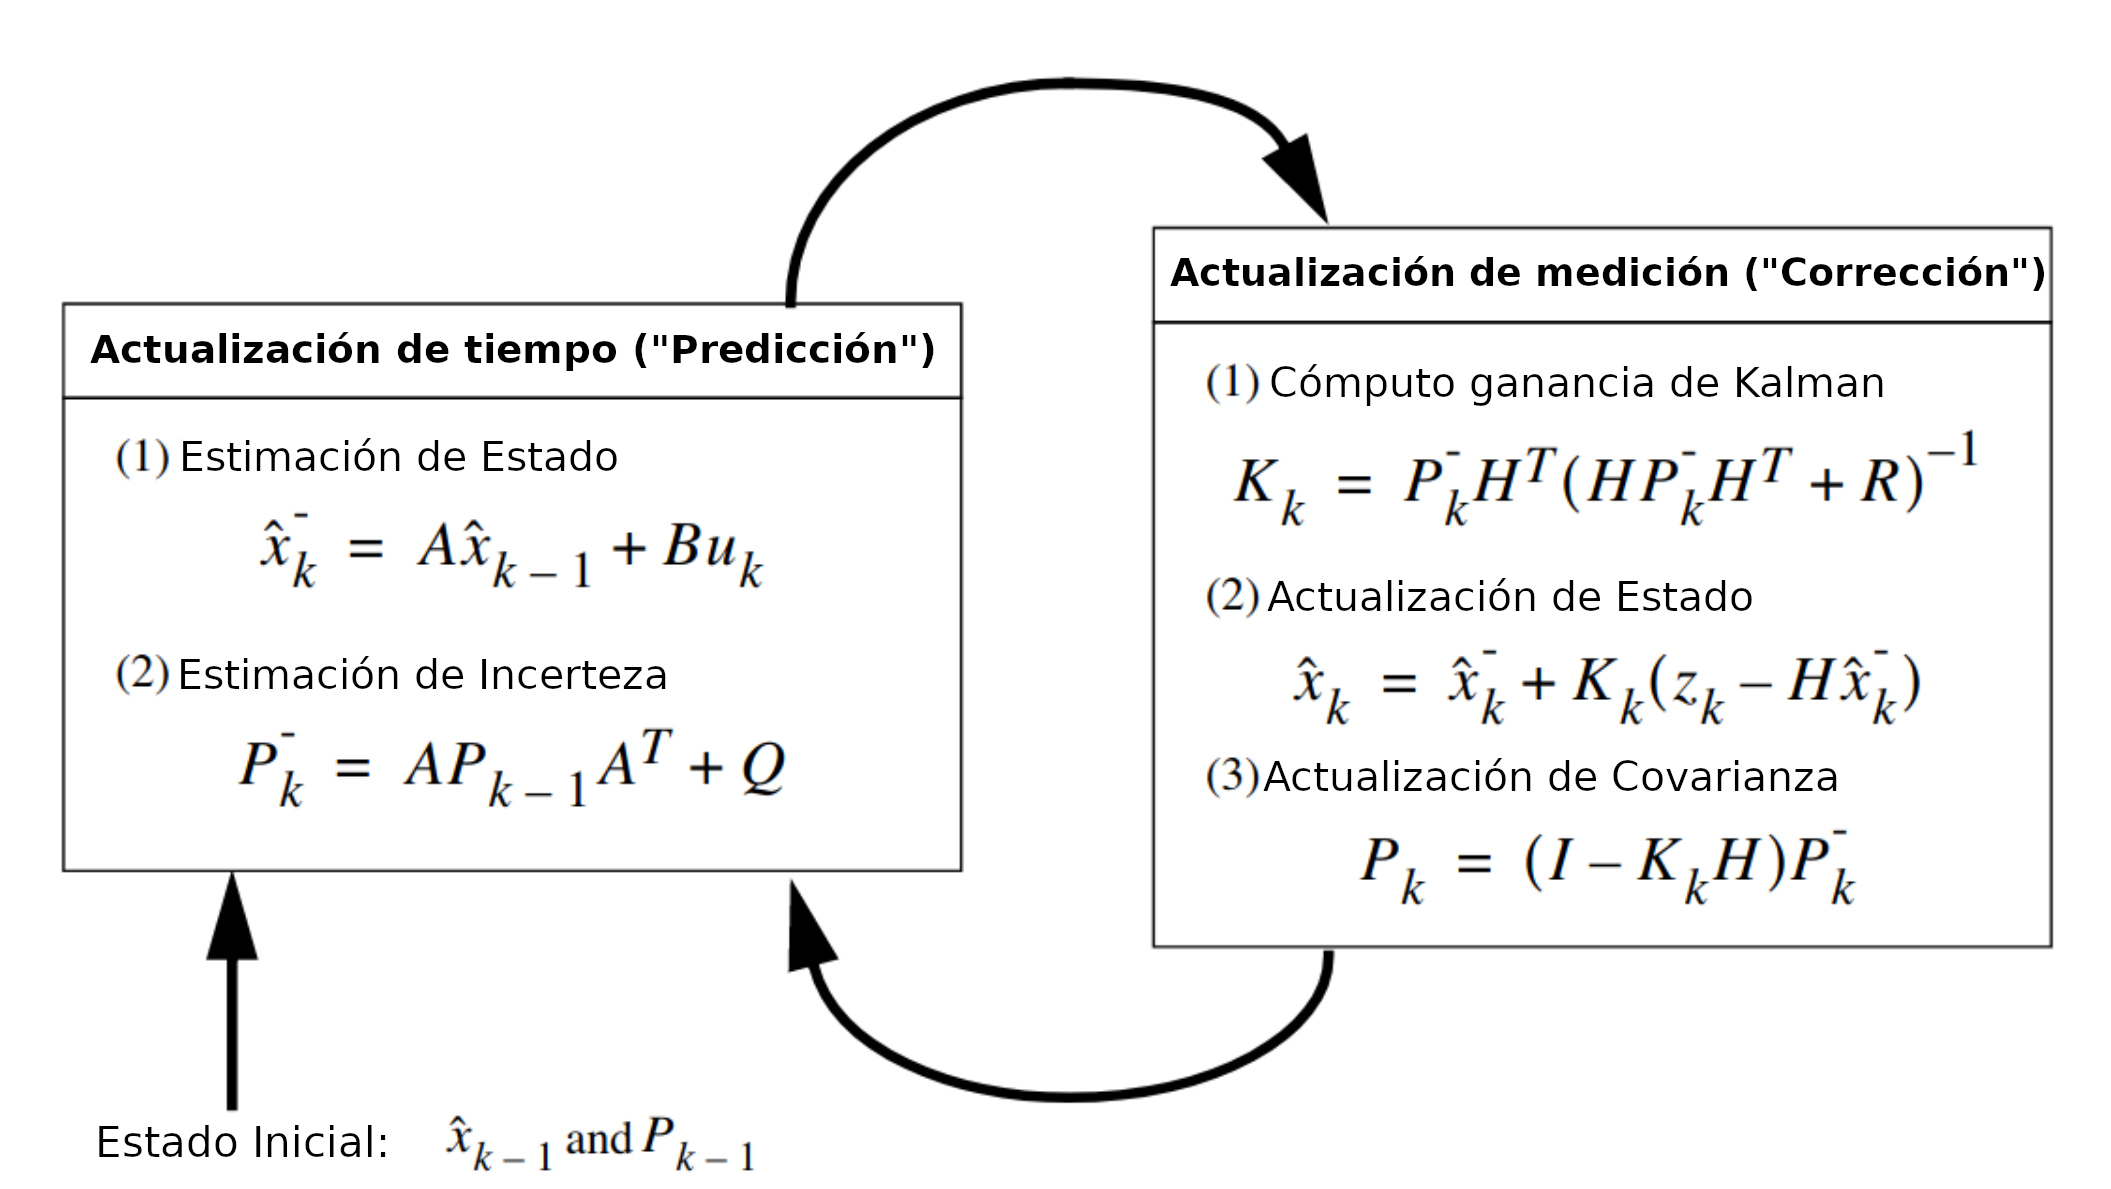
\includegraphics[width=0.7\textwidth]{kf_complete_esp.png}
        \caption{Diagrama detallado del funcionamieno del filtro de Kalman}
        \label{complete_kf}
    \end{center}
\end{figure}
\FloatBarrier

Resumiendo las matrices y vectores enunciadas en la Figura \ref{complete_kf}:

\begin{description}
    \item [$\mathbf{A_{k}}$]: Matriz de transición de estados. Es la matriz que
        relaciona $\mathbf{\hat{x}_{k}}$ con $\mathbf{\hat{x}_{k-1}}$.
    \item [$\mathbf{\hat{x}_{k}}$]: Estimado a priori del Vector de Estados.
    \item [$\mathbf{P_{k}}$]: Covarianza del error asociada a la estimación a priori.
    \item [$\mathbf{z_{k}}$]: Vector de mediciones al momento k.
    \item [$\mathbf{H_{k}}$]: Matriz de relación entre las mediciones z y el vector de
        estado al momento k.
    \item [$\mathbf{R_{k}}$]: Matriz de covarianza del ruido de las mediciones.
\end{description}

El desarrollo matemático completo del filtro de Kalman se incluye como apendice
en Anexo \ref{matKalman} para su consulta.

\noindent Este m\'etodo puede ser f\'acilmente utilizado para estimar el 
\acrshort{SOC} de una celda. En principio se necesita un modelo linealizado de la 
celda de litio-ion representado en un sistema de ecuaciones de estado e 
implementar el filtro para poder estimar el \acrshort{SOC} tomando una variable 
que se pueda utilizar y medir como salida para poder calcular un error de la 
estimaci\'on del estado, de forma tal que el algoritmo pueda iterar y calcular 
la ganancia de Kalman para \emph{corregir} su estimaci\'on.

\noindent Por ejemplo, en \cite{spagnol_kalman} se propone implementar un filtro 
de Kalman utilizando un modelo en ecuaciones de estado que permite fusionar la
representaci\'on de la celda en un modelo el\'ectrico (t\'ipico para
estimaci\'on del \acrshort{OCV}) con metodolog\'ias de conteo de Coulomb
(desarrollada en \ref{ahMethod}) obteniendo un m\'etodo que permite rechazar
tanto el ruido de las mediciones como tambi\'en errores param\'etricos del
modelo.

\noindent Los autores plantean el uso de un modelo el\'ectrico de la bater\'ia
basado en dos tanques RC conectados a una resistencia en serie y dos fuentes de
tensi\'on, controladas por el \acrshort{SOC}, que representa el \acrshort{OCV} 
de la celda durante el proceso de carga y descarga, como se puede observar en la 
Figura \ref{2rc_circuit}.

%\newpage

\begin{figure}[h!]
    \begin{center}    
        \begin{circuitikz}[american voltages]
            \draw (0, 0) to[D*] (0, -2);
            \draw (0, -2) to[cV, l=$OCV_{CC}(SoC)$] (0, -4);
            \draw (-1.5, -2) to[D*] (-1.5, 0);
            \draw (-1.5, -2) to[cV, l_=$OCV_{DC}(SoC)$] (-1.5, -4);
            \draw (-1.5, 0) to[short, -*] (0, 0);
            \draw (-1.5, -4) to[short, -*] (0, -4);
            \draw (0, 0) to[R=$R_0$] (2, 0);
            \draw (2, 0) to[short] (2, 1);
            \draw (2, 0) to[short] (2, -1);
            \draw (2, 1) to[R=$R_1$] (4, 1);
            \draw (2, -1) to[C=$C_1$] (4, -1);
            \draw (4, 1) to[short] (4, -1);
            \draw (4, 0) to[short] (5, 0);
            \draw (5, 1) to[short] (5, -1);
            \draw (5, 1) to[R=$R_2$] (7, 1);
            \draw (5, -1) to[C=$C_2$] (7, -1);
            \draw (7, 1) to[short] (7, -1);
            \draw (7, 0) to[short] (8, 0);
            \draw (0, -4) to[short] (8, -4);
            \draw (8, 0)  to[open, v=$v_o$] (8, -4);
        \end{circuitikz}
        \caption{Modelo el\'ectrico utilizado para representar la din\'amica de
        una celda de litio-ion}
        \label{2rc_circuit}
    \end{center}
\end{figure}
\FloatBarrier

\noindent Una vez caracterizado este modelo, se busca obtener un sistema de 
ecuaciones de estado para poder implementar el filtro de Kalman, partiendo desde 
la ecuaci\'on de la tensi\'on de salida, sobre un punto conocido del 
\acrshort{SOC}, con el objetivo de linealizarlo. Una vez planteado este sistema 
de ecuaciones, se puede proceder a implementar el Filtro de Kalman, donde su 
ganancia es recalculada para minimizar el error entre la tensi\'on de salida 
estimada con la obtenida en la medici\'on. 

\noindent Este procedimiento nos permite obtener un algoritmo apto para operar
en tiempo real bajo la aplicaci\'on de un veh\'iculo el\'ectrico, ya que no es
costoso de implementar a nivel de requerimiento computacional y solo depende de
dos sensores, un sensor de corriente y un sensor de tensi\'on que permita medir
ambas variables para fusionarlas dentro del algoritmo. Por \'ultimo, cabe
destacar que el mismo es robusto ante ruido en las mediciones, errores en la
parametrizaci\'on del modelo y error de inicializaci\'on, es decir, tener una
estimaci\'on err\'onea del estado incial del sistema. Esto se puede observar en
los resultados de la Figura \ref{resultados_soc_spagnoli}.

\begin{figure}[h!]
    \begin{center}
        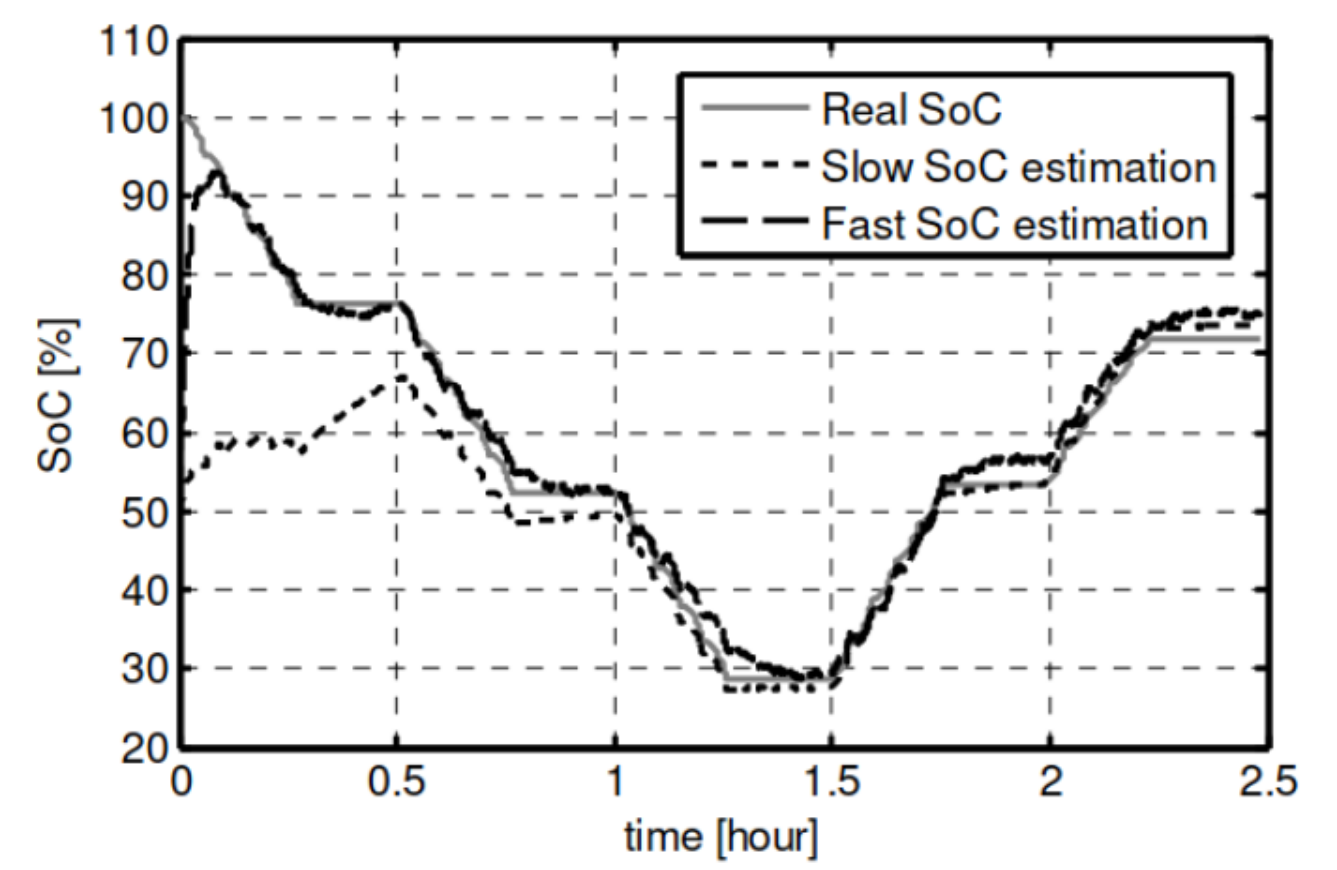
\includegraphics[width=0.7\textwidth]{soc_results_spagnoli.png}
        \caption{Resultados obtenidos en \cite{spagnol_kalman} sobre la
        estimaci\'on del Kalman con distintos par\'ametros de ajuste, con un
        \acrshort{SOC} inicial de un 50\%, se puede observar que la señal del
        \acrshort{SOC} converge a distintas velocidades al valor real.}
        \label{resultados_soc_spagnoli}
    \end{center}
\end{figure}

\noindent Los resultados de investigaciones relacionadas al Filtro de Kalman
como un observador del Estado de Carga obtuvieron resultados prometedores que
hacen que el algoritmo sea un gran candidato para sistemas en tiempo real, tales
como \acrshort{VVEE} o \acrshort{UPS}.

\subsubsection{M\'etodos basados en el aprendizaje autom\'atico}

\noindent El aprendizaje autom\'atico o, en ingl\'es, \acrfull{ML} surge como
una metodolog\'ia alternativa a la ingenier\'ia actual para el diseño de una
soluci\'on basado en un algoritmo. Como se ilustra en la Figura
\ref{curr_eng_approach}, el diagrama de flujo para el m\'etodo de ingenier\'ia
\emph{convencional} comienza con la \emph{adquisici\'on del conocimiento sobre
el tema}: El problema bajo estudio se analiza en detalle, produciendo un
\emph{modelo matem\'atico} que captura la \emph{f\'isica} del sistema,
identifica patrones de datos masivos y elaborar predicciones. Con este modelo,
se desarrolla un \emph{algoritmo optimizado} para el cálculo del \acrshort{SOC}
que ofrece determinado rendimiento asumiendo que el modelo f\'isico tiene un
cierto grado de exactitud en la representaci\'on de la realidad.

\begin{figure}[h!]
    \begin{center}
        \begin{tikzpicture}
            \draw (0, 0) rectangle (6, -.5);
            \draw (3, -.25) node {Adquicisi\'on de conocimientos};
            \draw [-stealth] (3, -.5) -- (3, -1.5);
            \draw (1, -1) node {Modelo Matem\'atico};
            \draw (0, -1.5) rectangle (6, -2);
            \draw (3, -1.75) node {Desarrollo del algoritmo};
            \draw [-stealth] (3, -2) -- (3, -3);
            \draw (3, -3.5) node {Algoritmo optimizado};
        \end{tikzpicture}
    \end{center}
    \caption{Diagrama de flujo convencional para el desarrollo de algoritmos}
    \label{curr_eng_approach}
\end{figure}

\noindent Por su contraparte, y en su forma m\'as b\'asica, el m\'etodo por
aprendizaje autom\'atico substituye el paso de la adquisici\'on del conocimiento
previo con la tarea de recoleccionar un gran conjunto de datos (o, en ingl\'es,
\emph{dataset}) con un comportamiento espec\'ifico del sistema a modelar. Este
conjunto de datos se lo denomina \emph{set de entrenamiento}. Como se puede
observar en la Figura \ref{ml_approach}, el set de datos sirve como información
de entrada del algoritmo de aprendizaje que, como resultado, producirá una
\emph{m\'aquina} entrenada para llevar adelante la tarea deseada. En nuestro
caso el cálculo del \acrshort{SOC} del pack de batería. El aprendizaje es
realizado a trav\'es de un conjunto de algoritmos, tambi\'en conocidos como
\emph{hip\'otesis}, a partir de la toma la decisi\'ones ante estímulos obtenídos
del dataset. Los algoritmos de aprendizaje est\'an generalmente basados en la
optimizaci\'on de un criterio que mide cuan bien se desempeña el algoritmo de
aprendizaje seleccionado para la tarea a la que fue diseñado.

\begin{figure}[h!]
    \begin{center}
        \begin{tikzpicture}
            \draw (0, 0) rectangle (6, -.5);
            \draw (3, -.25) node {Adquicisi\'on de datos};
            \draw [-stealth] (3, -.5) -- (3, -1.5);
            \draw (1, -1) node {Set de entrenamiento};
            \draw (0, -1.5) rectangle (6, -2);
            \draw (3, -1.75) node {Aprendizaje};
            \draw [-stealth] (3, -2) -- (3, -2.5);
            \draw (3, -2.75) node {Algoritmo};
            \draw [-stealth](-1, -1.75) -- (0, -1.75);
            \draw (-2, -1.75) node {Hip\'otesis};
        \end{tikzpicture}
    \end{center}
    \caption{Diagrama de flujo b\'asico para la generaci\'on de un modelo
    utilizando aprendizaje autom\'atico}
    \label{ml_approach}
\end{figure}

T\'ecnicas m\'as avanzadas del aprendizaje autom\'atico integran conocimientos
disponibles sobre el problema dentro del proceso de aprendizaje para lograr un
algoritmo m\'as robusto, esto suele ser aplicado, por ejemplo, en aplicaciones
para el procesamiento de im\'agenes donde el conocimiento sobre la invarianza
translacional de las caracter\'isticas visuales son utilizadas para adoptar
redes neuronales convolucionales (\acrshort{CNN}, del ingl\'es 
\emph{\acrlong{CNN}}) como hip\'otesis para ser entrenadas. Generalmente, como
se muestra en la Figura \ref{ml_ext_approach}, el conocimiento previo al
problema puede dictar la elecci\'on de hip\'otesis espec\'ificas para el uso
durante el proceso de entrenamiento. 

\begin{figure}[h!]
    \begin{center}
        \begin{tikzpicture}
            \draw (0, 0) rectangle (6, -.5);
            \draw (3, -.25) node {Adquicisi\'on de datos};
            \draw [-stealth] (3, -.5) -- (3, -1.5);
            \draw (1, -1) node {Set de entrenamiento};
            \draw (0, -1.5) rectangle (6, -2);
            \draw (3, -1.75) node {Aprendizaje};
            \draw [-stealth] (3, -2) -- (3, -2.5);
            \draw (3, -2.75) node {Algoritmo};
            \draw [-stealth](-1.5, -1.75) -- (0, -1.75);
            \draw (-0.75, -2.25) node {Hip\'otesis};
            \draw (-6, -1.5) rectangle (-1.5, -2);
            \draw (-3.75, -1.75) node {Conocimiento del problema};
        \end{tikzpicture}
    \end{center}
    \caption{Diagrama de flujo para la generaci\'on de un algoritmo 
    utilizando aprendizaje autom\'atico y conocimientos del problema}
    \label{ml_ext_approach}
\end{figure}
\FloatBarrier

\noindent Dentro de la literatura que utiliza algoritmos de aprendizaje
autom\'atico para la estimaci\'on del \acrshort{SOC}, se propone el uso de
varias hip\'otesis detalladas a continuaci\'on,

\subsubsubsection{Redes Neuronales Artificiales}

\noindent Las redes neuronales artificiales (\acrshort{ANN}, del ingl\'es
\emph{\acrlong{ANN}}) tienen la capacidad de aprendizaje y adaptaci\'on para
poder representar un modelo no-lineal de gran complejidad. Las \acrshort{ANN}
puede usar un set de datos de entrenamiento para estimar el \acrshort{SOC} sin
conocer informaci\'on sobre la estructura interna de la bater\'ia ni el
\acrshort{SOC} inicial. Generalmente, se requieren al menos tres capas para
formar el algoritmo, incluyendo la capa de entrada, una o m\'as capas ocultas y
la capa de salida. La estructura de una \acrshort{ANN} para estimar el
\acrshort{SOC} se puede observar en la Figura \ref{ann_soc_layers}.

\begin{figure}[h!]
    \begin{center}
        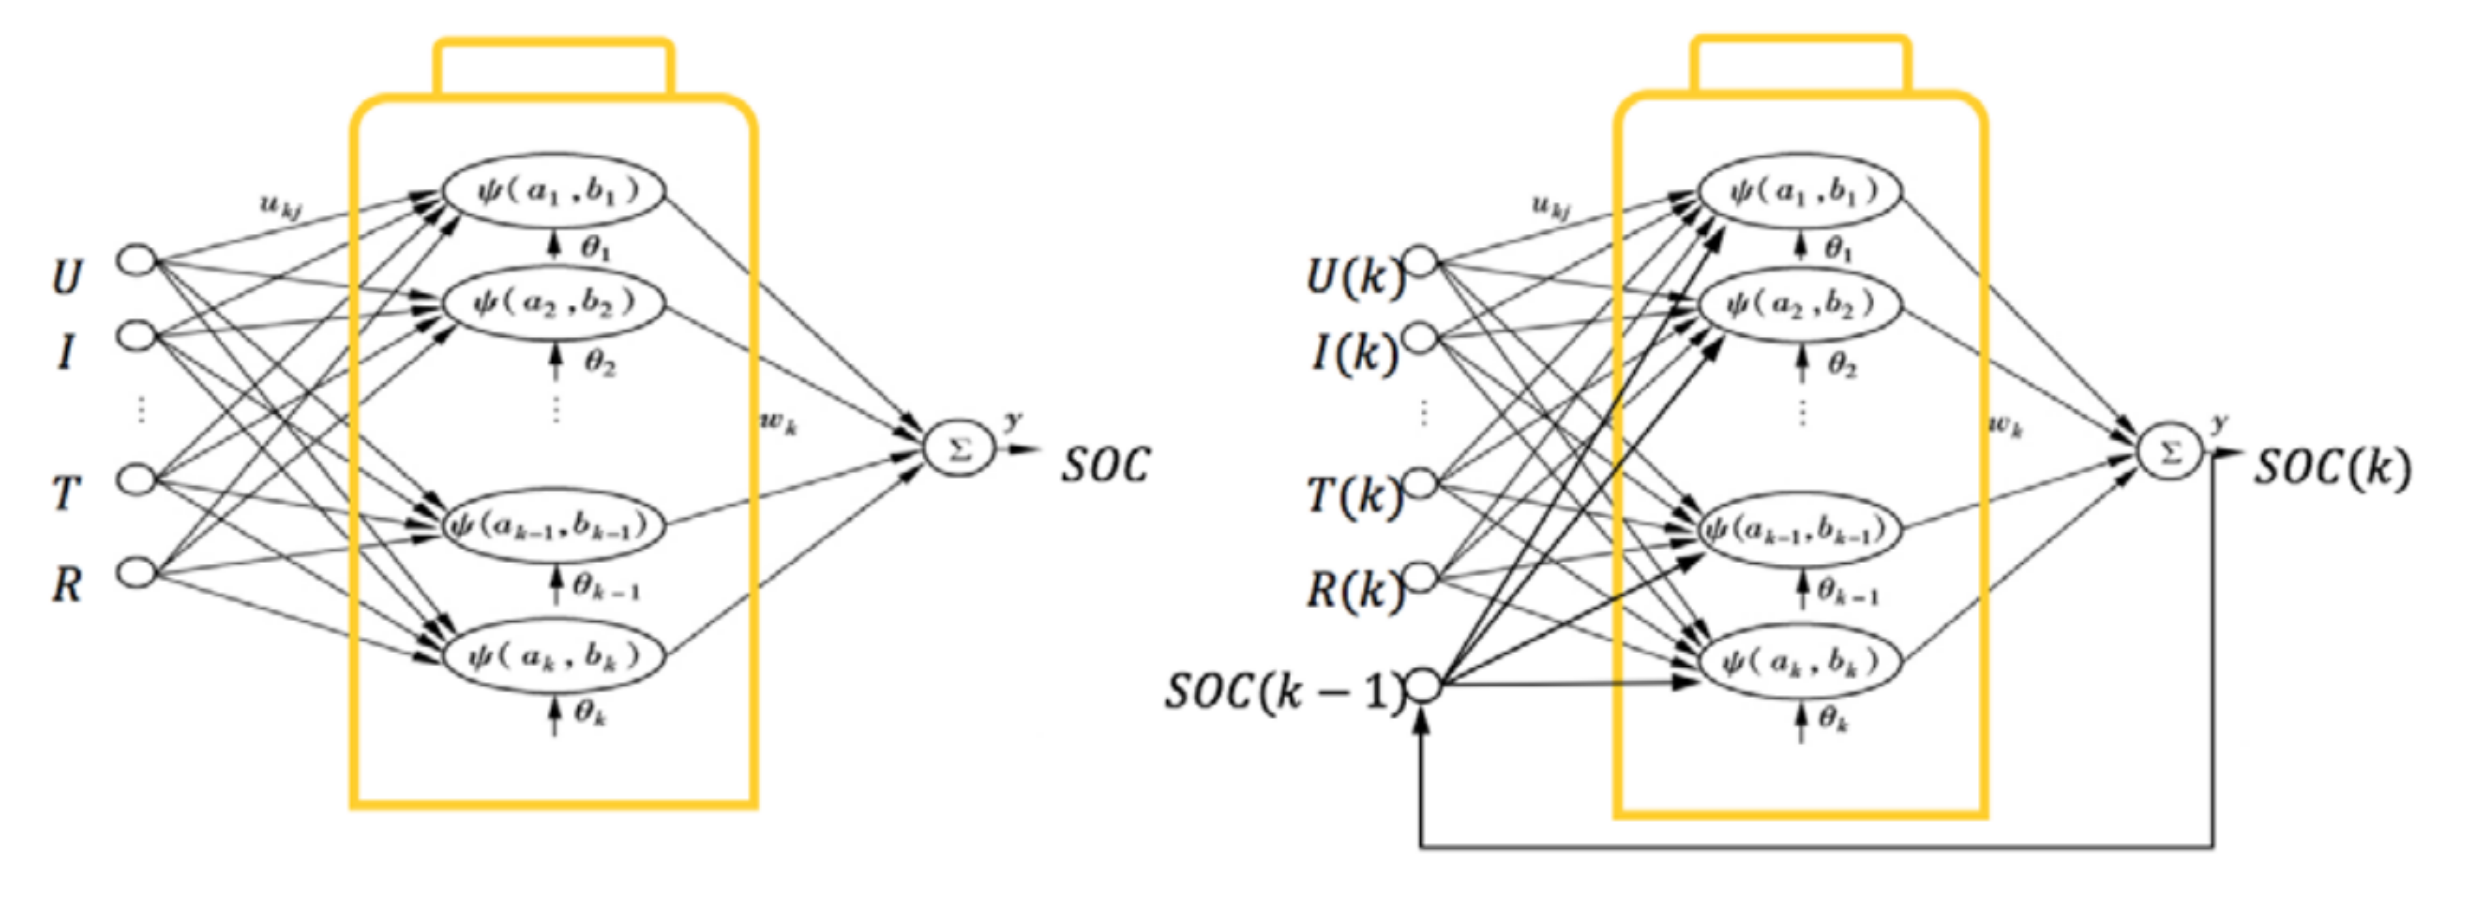
\includegraphics[width=1\textwidth]{ann_soc.png}
        \caption{Estrucutra de una \acrshort{ANN} para la estimaci\'on del
        \acrshort{SOC}}
        \label{ann_soc_layers}
    \end{center}
\end{figure}

\noindent \'Este m\'etodo utiliza el voltaje de la terminal, la corriente de
carga y descarga, y la temperatura ambiental como la entrada y la salida del
algoritmo es el \acrshort{SOC}. En \cite{XIA2018694} se propone el algoritmo
de Levenberg-Marquardt, una red neuronal optimizada basada en \emph{wavelets}.
En \cite{DANG2016356} se propone una red neuronal dual fusionada con un modelo 
de la bater\'ia para estimar el \acrshort{SOC}. Por el otro lado, 
\cite{TONG2016236} propone una nueva arquitectura para la estimaci\'on 
\acrshort{SOC} usando una red neuronal para clasificaci\'on de carga alcanzando 
un error de un 3.8\% en promedio. La gran ventaja de este m\'etodo es que puede 
operar bajo condiciones no-lineales obteniendo resultados \'optimos para su 
aplicaci\'on. Sin embargo, el algoritmo necesita un gran set de datos de 
entrenamiento, que no solo requiere gran poder computacional para poder 
entrenarlo, si no que tambi\'en un gran espacio de almacenamiento por lo cual su 
desarrollo es costoso si el presupuesto es limitado.

\newpage

\subsubsubsection{M\'aquinas de Vectores de Soporte}

\noindent El m\'etodo basado en las M\'aquinas de Vectores de Soporte 
(\acrshort{SVN} del ingl\'es \acrlong{SVN}) utiliza el algoritmo de regresi\'on 
lineal para transformar un modelo de baja dimensi\'on ($\mathrm{R^m}$) a otro de 
alta dimensi\'on ($\mathrm{R^n}$). \acrshort{SVM} fue diseñado, en principio, 
para  resolver problemas no-lineales de clasificaci\'on de dos clases. El punto 
clave de este m\'etodo es relacionar la muestra original del modelo de bajas 
dimensiones a uno de un espacio con mayores dimensiones encontrando un plano que 
puede separar ambas muestras de dos clases distintas, como se puede observar en 
la Figura \ref{svn_graph}

\begin{figure}[h!]
    \begin{center}
        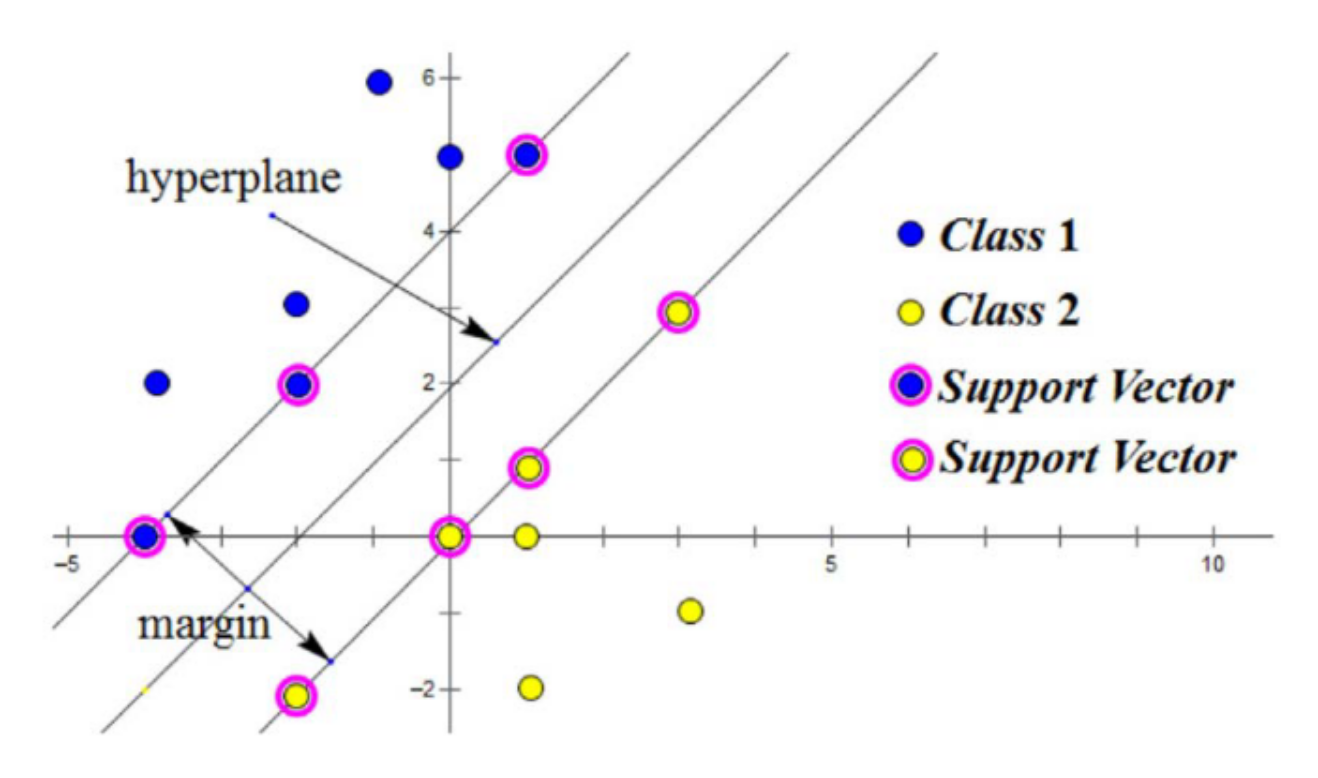
\includegraphics[width=.7\textwidth]{svm_graphic.png}
        \caption{Hiperplano que separa ambas clases}
        \label{svn_graph}
    \end{center}
\end{figure}

\noindent En \cite{HU2014682} se propone estimar el \acrshort{SOC} basado en 
\acrshort{SVM} optimizado para regresiones con un proceso de optimizaci\'on de 
doble b\'usqueda, utilizando

\noindent La arquitectura \acrshort{SVM}, tiene la habilidad de tolerar el ruido 
y escalar para integrar conocimientos de otros indicadores, tales como la 
temperatura, la energ\'ia entregada/consumida, entre otras variables de 
inter\'es. Sin embargo, este m\'etodo consume una gran cantidad de tiempo lo que 
lo imposibilita para funcionar en un sistema en tiempo real.

\subsubsubsection{L\'ogica Difusa}

\noindent La l\'ogica difusa (\acrshort{FL}, del ingl\'es \acrlong{FL}) es un
algoritmo utilizado para generar modelos complejos no-lineales con la ayuda de
un set de datos de entrenamiento. En este caso, \cite{DAI2015350} propone un 
algoritmo para la estimaci\'on del \acrshort{SOC} de forma \emph{online},
combinando un estimador cl\'asico del \acrshort{SOC} con un sistema fuzzy de
inferencia adaptativo (\acrshort{ANFIS}, del ingl\'es \acrlong{ANFIS}). \'Este
m\'etodo es propicio para adaptarse a distintas condiciones de operaci\'on de la
bater\'ia incluyendo el proceso de envejecimiento. La Figura \ref{anfis_arch}
ilustra una estructura b\'asica \acrshort{ANFIS} con cinco capas.

\begin{figure}[h!]
    \begin{center}
        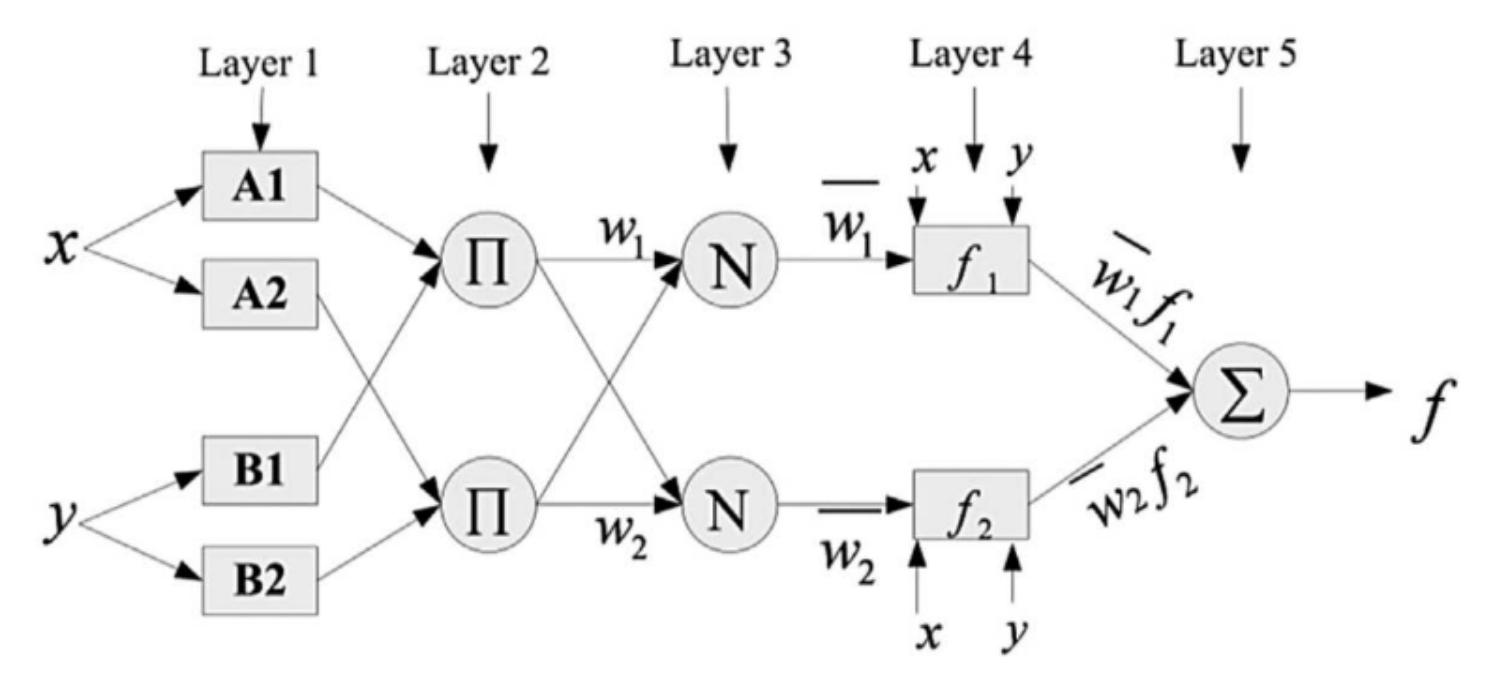
\includegraphics[width=0.8\textwidth]{anfis_arch.png}
        \caption{Arquitectura b\'asica para un \acrshort{ANFIS} de cinco capas}
        \label{anfis_arch}
    \end{center}
\end{figure}

\noindent A pesar de que la \acrshort{FL} tiene una poderosa habilidad para 
predicir modelos no lineales, la misma requiere algoritmos computacionales 
complejos y unidades de memorias de almacenamiento lo suficientemente amplios, 
logrando que el sistema sea excesivamente costoso para determinadas 
aplicaciones.

\newpage

\subsubsection{Algoritmo de Estimaci\'on}

\noindent La Figura \ref{comp_error_soc} demuestra la complejidad computacional 
en base al error en la estimaci\'on sobre los m\'etodos de estimaci\'on de 
\acrshort{SOC}.

\noindent En el presente, la estimaci\'on con mayor potencial y usado
ampliamente dentro de los \acrshort{BMS} es la combinaci\'on entre el modelo
el\'ectrico equivalente y un filtro de Kalman. El error m\'as significativo de
este m\'etodo proviene de los sensores de voltaje y corriente y no de la
influencia de los efectos intr\'insecos de la bater\'ia, como por ejemplo, el
envejecimiento, la temperatura y el efecto de hist\'erisis.

\begin{figure}[h!]
    \begin{center}
        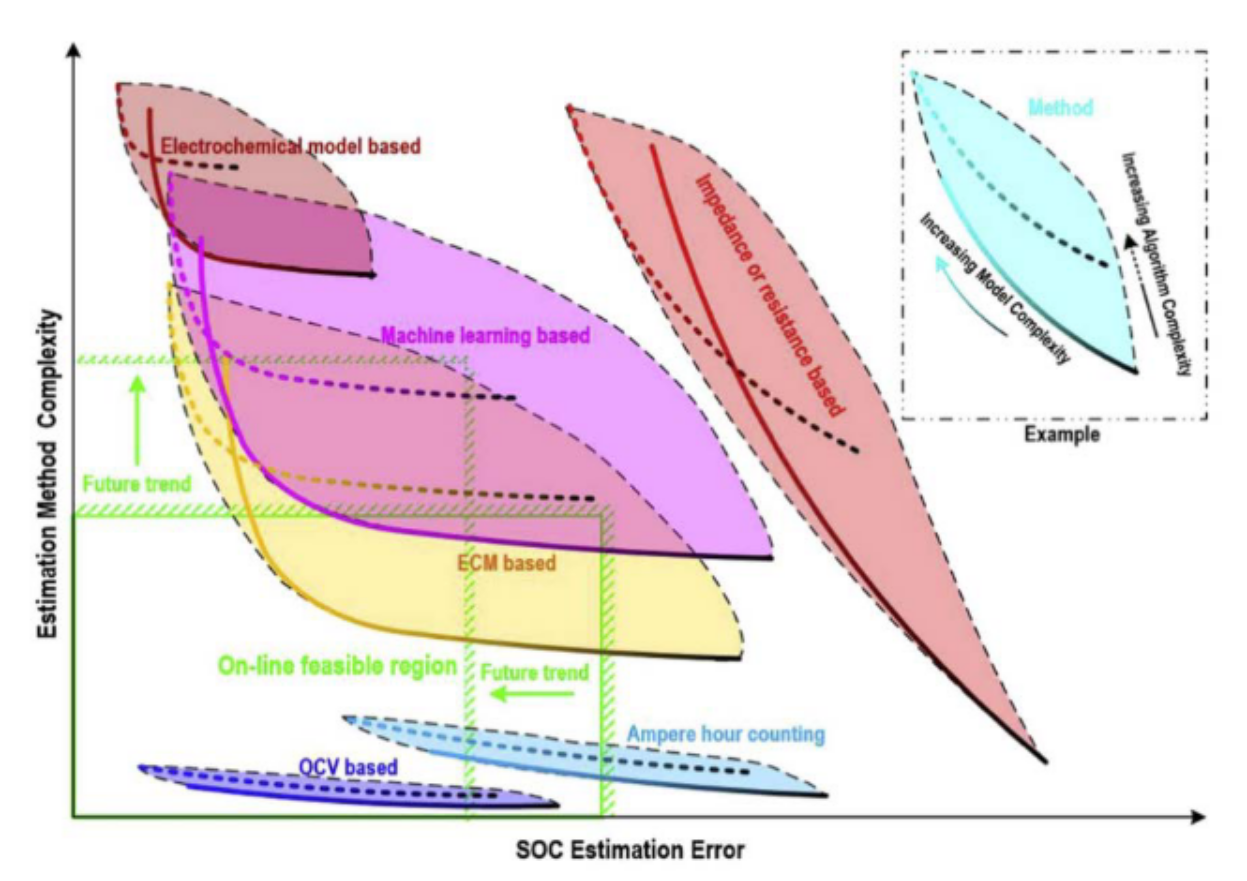
\includegraphics[width=0.8\textwidth]{comparisson_soc.png}
        \caption{Gr\'afica comparando los m\'etodos en base a la complejidad y
        exactitud}
        \label{comp_error_soc}
    \end{center}
\end{figure}

\subsection{Proceso de Carga}\label{sec:tecnica_carga}

El proceso de carga de una \acrfull{Ion-Li} no es trivial. Aplicar una tensión
constante en  bornes, como podríamos proceder con baterías de plomo ácido, no es
el procedimiento más adecuado en este caso. En aras de optimizar la autonomía y
la vida útil del pack de baterías el proceso de carga debe responder a
lineamientos particulares de acuerdo a las carácterísticas constructivas de las
celdas que lo componen. Este proceso est\'a descripto por un perfil de Corriente
Constante (CC) - Voltaje Constante (CV)

\subsubsection{Corriente Constante CC - Voltaje Constante CV}

El perfil de carga que se ajusta a las celdas de \acrshort{Ion-Li}, como se
observa en la figura \ref{fig:char_prof}, es el perfil \acrshort{CC} -
\acrshort{CV}. Este consiste en tres fases, una primera etapa de
acondicionamiento o pre carga donde se inyecta a la batería una corriente
constante pequeña de magnitud equivalente a la corriente de fin de carga. Una
fase de carga rápida a corriente constante \acrshort{CC} y una tercer y última
fase de carga a tensión constante \acrshort{CV}.

\begin{figure}[h!] \centering
    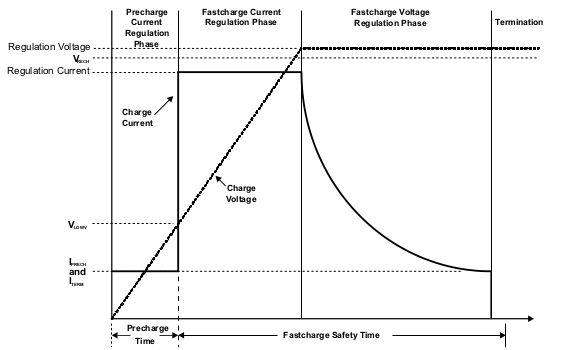
\includegraphics[width=0.8\textwidth]{bat_char/char_profile.png}
    \caption{Perfil de carga típico de una batería de Ion-Litio}
\label{fig:char_prof} \end{figure} \FloatBarrier

El proceso de pre-carga o pre-acondicionamiento proporciona a las celdas la
capacidad de recuperar su capa de pasivación, la cual puede haberse visto
afectada o disuelta tras largos per\'iodos de almacenamiento en estados de
descarga profunda. A su vez permite introducir las celdas en la zona de
operación segura en caso de que se encuente profundamente descargadas. Es
importante limitar el proceso de acondicionamiento en tiempo para prevenir 
pre-cargar indefinidamente una celda que se encuentre agotada. Si tras un 
periodo completo de acondicionamiendo la celda no alcanza el voltaje mínimo 
necesario puede considerarse que la misma alcanzó el final de su vida útil.

El voltaje umbral de inicio de carga rápida depende de la composici\'on
qu\'imica de la celda y en el caso de las baterías litio-ion, la misma 
se ubica generalmente entre los 2.5V y 3.0V. Una vez que la celda supera su 
voltaje umbral mínimo el cargador deber\'a entrar en la zona de carga rápida, es
decir, en la etapa de corriente constante \acrshort{CC}. La fase de carga rápida 
permite a la batería transformar la enería eléctrica entregada en energía 
electroquímica dentro de la batería en el menor tiempo posible. La magnitud de 
la corriente de carga rápida depende de la celda y es limitada generalmente 
entre 0.5C y 1C para prevenir el calentamiento del pack y su degradación 
prematura. El pack de batería admitirá carga rápida a corriente constante hasta 
alcanzar el voltaje límite de regulación. 

En esta tercer, y última fase, la corriente drenada del pack decae
exponencialmente hasta alcanzar la magnitud de fin de carga, situación que nos
indica que el ciclo se completo exitosamente. La corriente de terminación de
carga ronda entre 5\% y 10\% de la corriente de carga rápida. Cabe aclarar
que en esta instancia del proceso de carga la corriente decae naturalmente dado
que la magnitud controlada por el cargador es la tensi\'on en bornes de la
celda.  

Es importante remarcar que durante todo el proceso de carga, 
fundamentalmente durante la fase de carga rápida a corriente constante, es de
vital importancia monitorear la temperatura de las celdas evitando que las
mismas se aparten de la zona de operación segura, ya que el proceso de carga
implica intrínsicamente una elevación de la temperatura de la celda, entre otras
causas, debido a su resistencia interna.

El tiempo total de carga es una variable determinante a la hora de implementar
un cargador de batería que extienda al máximo la vida útil y los ciclos de carga
de un pack de baterías y de sus celdas. Es la magnitud de corriente de carga
rápida la variable determinante de este tiempo. Por ejemplo, para una
carga rápida a 1C, la batería alcanzará, durante la fasé de \acrshort{CC}, el
$70\%$ de su capacidad total en el $30\%$ del tiempo de carga mientras que
tardará el $70\%$ del tiempo total de carga para acumular el $30\%$ restante de
su capacidad durante la fase \acrshort{CV}. 

La existencia de una resistencia interna en serie en las celdas no ideales
implica que a mayor corriente de carga rápida a CC se alcance más rápido la
tensión de umbral de paso a la fase de tensión constante CV acortando el tiempo
de CC pero extendiendo el tiempo de CV. Podemos inferir entonces que a menor
resistencia interna menor tiempo de carga. Y que aumentar la corriente a CC
tambien reducirá el tiempo de carga.  Sin embargo, se desaconseja completamente
implementar regímenes de carga rápida que superen 1C por el impacto en el número
de ciclos de vida útil de las celdas del pack de batería. La figura
\ref{fig:C_vs_Cycle_I} muestra como a medida que aumentamos el régimen de carga
de una celda la vida \'util de la misma, medido en ciclos de carga, disminuye
significativamente.

\begin{figure}[h!] \centering
    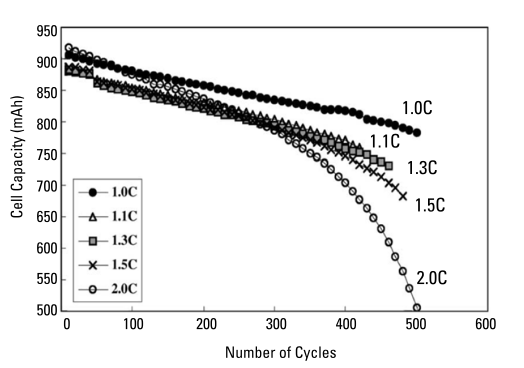
\includegraphics[width=0.6\textwidth]{bat_char/C_vs_Cycle_I.png}
    \caption{Relación Corriente de carga vs Ciclos de vidaútil de una celda de
    Ion-Litio con un cátodo de $LiCoO_2$} \label{fig:C_vs_Cycle_I} 
\end{figure}
\FloatBarrier

A mayores tasas de corriente, mayor cantidad de iones de litio se depositan
sobre el ánodo conviritiendose en litio metálico al librerar sus electrónes
disponibles.  El litio metálico es sumamente reactivo con el electrolito
resultando en una pérdida permanente de \acrshort{Ion-Li}, el elemento
almacendor de la energía, acelerando el envejecimiento prematuro de la celda y
en consecuencia reduciendo los ciclos de vida útiles de la misma. 

Normalmente, a mayor voltaje en bornes de una celda mayor es la capacidad de la
misma. Podríamos entonces vernos tentados a aumentar el voltaje límite de
regulación y sobre cargar una celda para aumentar la carga almacenada. Por
ejemplo, una celta cargada a $4.3V$ en vez de $4.2V$ va a permitirnos almacenar
un $10\%$ más de carga inicial. El inconveniente aqui reside nuevamente en el
impacto que tendra este procedimiento en el número de ciclos de carga y la vida
útil de la celda. La vida útil de una celda sobrecargada se vería reducida en
un $50\%$.  Por el otro lado, cargar una celda con un un voltaje menor ($40mv$
menor) implicará una reducción aproximada de un $10\%$ de su carga inicial.
Podemos arribar a la conclusión que el control del voltaje de carga y su
precisión es de vital importancia en un circuito de carga. La figura
\ref{fig:C_vs_Cycle_V} muestra la relación entre el número de ciclos de carga y
los diferentes voltajes de carga. 

\begin{figure}[h!] \centering
    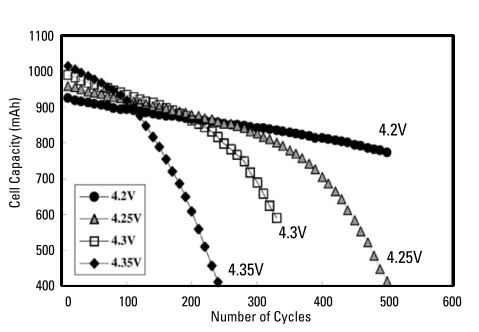
\includegraphics[width=0.6\textwidth]{bat_char/C_vs_Cycle_V.png}
    \caption{Relación Voltaje de carga la batería vs Ciclos de vida de una celda de
Ion-Litio con un cátodo de $LiCoO_2$} \label{fig:C_vs_Cycle_V} \end{figure}
\FloatBarrier

A voltajes mayores el material del cátodo reacciona a mayor velocidad con el
electrolito perdiéndose material en la reacción resultando en una perdida de
capacidad de almacenamiento de energía. Sumado al control del proceso de carga,
tambi\'en se debe monitorear sobre el mismo la ecualizaci\'on de las celdas en
caso de que el pack de bater\'ias posea una arquitectura con mayor cantidad de
celdas conectadas en serie.

\subsection{Ecualización de celdas}

Los packs de bater\'ias en los \acrshort{VVEE} consisten de un gran n\'umero de
celdas agrupadas en serie y en paralelo para proveer la suficiente energia y
potencia al veh\'iculo. Sin embargo, las caracter\'isticas internas de la
bater\'ia incluyendo capacidad inicial, impedancia interna, volumen f\'isico,
corriente de auto-descarga, etc., y condiciones externas, tales como la
temperatura ambiental, son siempre inconsistentes en la vida real. Al nivel del
pack de bater\'ias, las variaciones de par\'ametros entre celdas en serie puede
llevar a una degradaci\'on acelerada del mismo, con un impacto negativo en la
potencia, capacidad, tiempo de vida restante, entre otras limitaciones. El
desbalance puede deteriorar este degradamiento al punto de poner en riesgo al
veh\'iculo desencadenando un embalamiento t\'ermico del pack. Por lo tanto, la
ecualizaci\'on del pack de bater\'ias, que puede mejorar la seguridad y
rendimiento del mismo es una tecnolog\'ia cr\'itica dentro del \acrshort{BMS}
para la reducci\'on del desbalance entre celdas.

La ecualizaci\'on tambi\'en es cr\'itica para un segundo uso de celdas de
litio-ion que se encuentra en desuso. Las bater\'ias con una capacidad degradada
en un 20\% deber\'ian ser reemplazadas para garantizar seguridad y autonom\'ia
al \acrshort{VE}. Reacondicionando celdas en desuso para bicicletas
el\'ectricas, veh\'iculos el\'ectricos de excursi\'on y sistemas de
almacenamiento de energ\'ia, pueden generar beneficios tanto ambientales como
econ\'omicos, y esto es posible gracias a una eficiente ecualizaci\'on de las
celdas.

Los circuitos de ecualizaci\'on, o \emph{ecualizadores}, combinados con
estrategias de ecualizaci\'on pueden ayudar evitar el problema del desbalanceo
dentro del pack de bater\'ias. A pesar de que distintas aplicaciones de
\acrshort{VE} tienen distintos requerimientos, la topolog\'ia del diseño del
hardware est\'a limitado por el costo, tamaño y fiabilidad. A pesar del progreso
dentro de esta tecnolog\'ia, las soluciones existentes no puede resolver todos
los requerimientos de estos sistemas. Por lo tanto, es esencial primero
describir los motivos de las inconsistencias entre celdas y el estado de arte de
la tecnolog\'ia actual para el diseño del \acrshort{BMS}

\newpage

\subsubsection{Inconsistencias entre celdas}

Para satisfacer la demanda de voltaje, potencia y energ\'ia en los 
\acrshort{VVEE}, los packs de bater\'ia contienen desde decenas hasta miles de
celdas conectadas en serie o en paralelo y, las inconsistencias entre ellas son
inevitables por una gran cantidad de motivos. Uno de los primeros problemas que
traen estas inconsistencias es que la capacidad del pack de bater\'ias est\'a
limitado por la celda de menor capacidad, este defecto tienen un nombre y es el
\emph{efecto barril}, el mismo se puede visualizar en la Figura 
\ref{barrel_effect}A, en este caso el pack de bater\'ias cesar\'a la descarga del
pack si cualquiera de las celdas alcanza el fin de la descarga. De forma
similar, la carga disponible del pack de bater\'ias, como se puede observar en
la Figura \ref{barrel_effect}B, est\'a limitado por la celda con menor
capacidad, donde el pack finalizar\'a el proceso de carga si cualquiera de las
celdas alcanza el final de carga. Por lo tanto, la capacidad de carga/descarga
del pack est\'a fuertemente influenciado por estas inconsistencias.

Sumado a eso, estas inconsistencias son variantes en el tiempo y asociadas a
varios factores, especialmente con la degradaci\'on del pack. Las
caracter\'isticas no lineales del envejecimiento de las celdas de litio-ion
afectar\'an gradualmente la inconsistencia del pack. A pesar de que las celdas
pueden tener un desapareamiento de capacidad inicial de un 3\%, esta
inconsistencia no puede ser eliminada y tiene una tendencia a empeorar llevando
a una degradaci\'on prematura y aumentar los riesgos de sobrecarga/descarga
durante cada ciclo llegando finalmente a un embalamiento t\'ermico.

Los or\'igenes de las inconsistencias pueden ser separados en dos grupos: el
proceso de producci\'on y el uso de las mismas. El primero puede ser causado por
variaciones en los materiales, equipo de producci\'on y procedimientos, que
llevan a una inconsistencia en los par\'ametros entre celdas del mismo modelo.
Mientras que el segundo est\'a fuertemente relacionado con las diferencias
ambientales durante el uso y almacenamiento de las bater\'ias. Ambas
inconsistencias influyen directamente sobre el rendimiento del pack de
bater\'ias.


\begin{figure}[h!]
    \begin{center}
        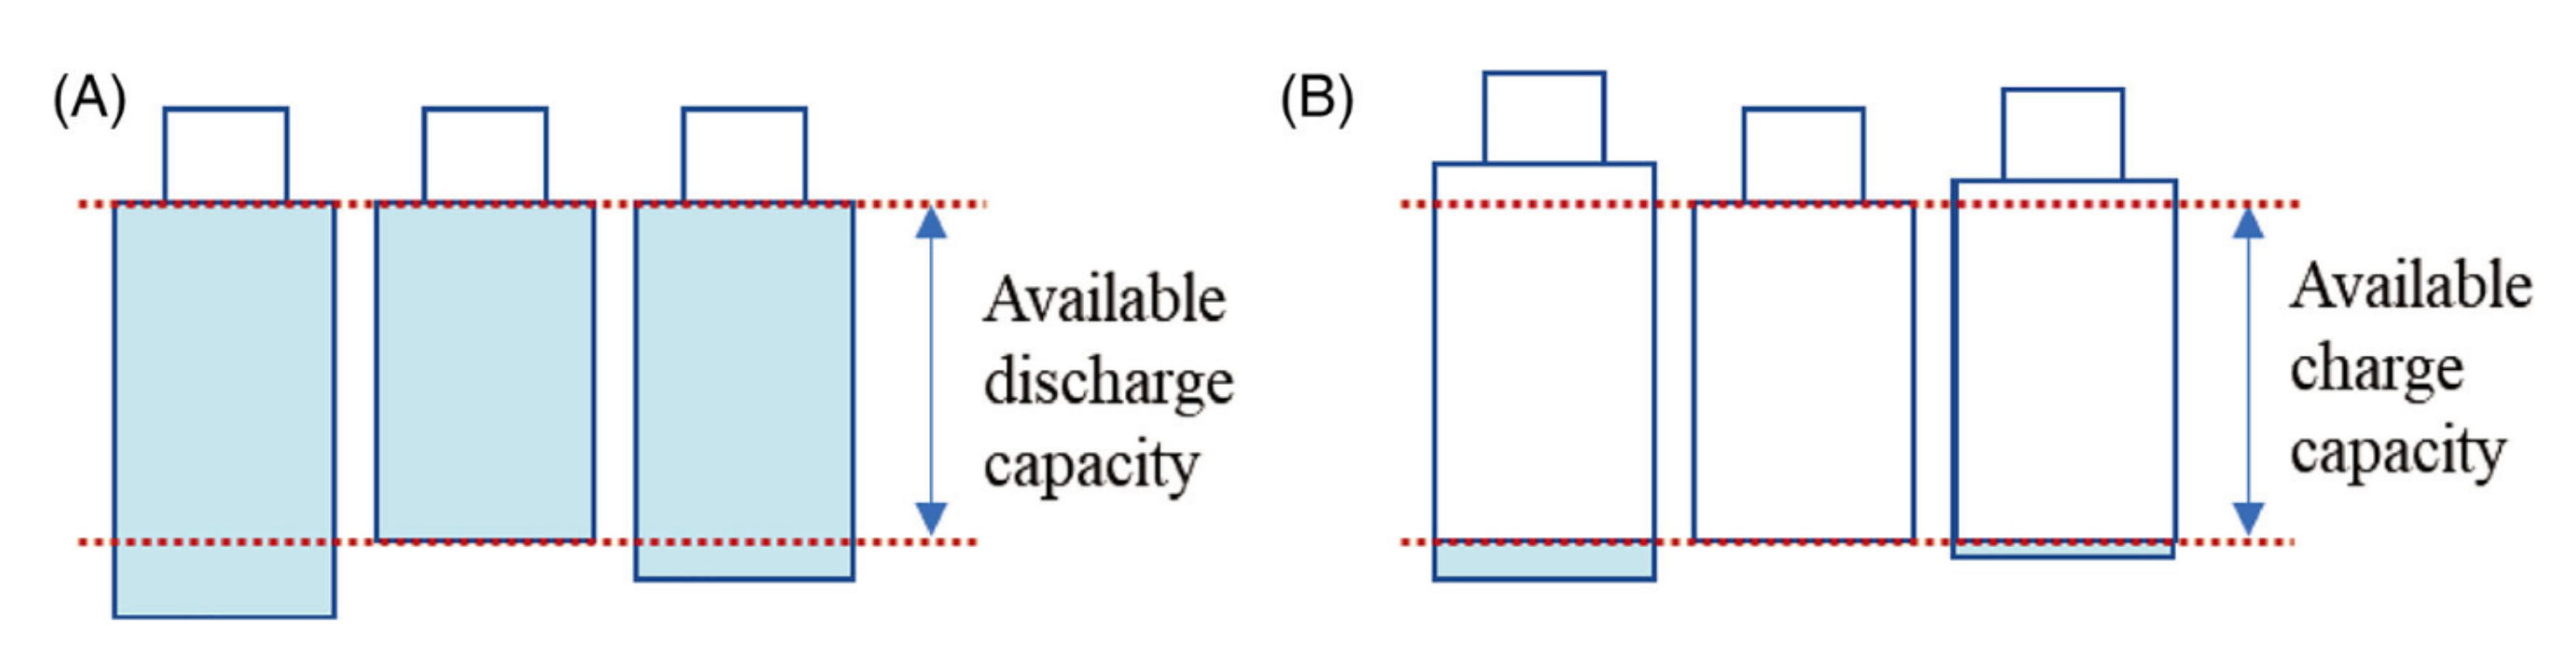
\includegraphics[width=1\textwidth]{barrel_effect.png}
        \caption{(A) Capacidad de descarga disponible. (B) Capacidad de carga
        disponible}
        \label{barrel_effect}
    \end{center}
\end{figure}

\subsubsubsection{Inconsistencias causadas por la producci\'on}

El proceso de producci\'on de las celdas de litio-ion consiste en mezclar
materiales acuosos, cubrir, cortar, devanar, ensamblar e inyectar electrolito,
donde cada paso puede provocar variaciones y afectar la inconsistencia en la
producci\'on de los distintos lote. Por ejemplo, la mezcla no uniforme de las
sustancias puede provocar defectos sutiles en la microestructura de la celda,
que afecta de forma directa al rendimiento de las mismas. Debido a las
diferencias en el material, precisi\'on en los equipos y la incerteza del
proceso de producci\'on, las diferencias entre baches de producci\'on son
inevitables. La otra influencia de heterogeneidad inicial incluye a la capacidad
inicial y a la resistencia interna, concentraci\'on de litio-ion, grosor del
separador entre otros.

Las inconsistencias causadas por el proceso de producci\'on no pueden ser
eliminadas por completo. Sin embargo, se pueden utilizar m\'etodos de
apareamiento a la hora de ensamblar el pack de bater\'ias para combinar aquellas
que sean consistentes entre s\'i, mejorando la fiabilidad, seguridad y tiempo de
vida de un pack de bater\'ias. \'Estos m\'etodos se basan en criterios tales
como la capacidad, la resistencia interna y la corriente de auto-descarga.

\subsubsubsection{Inconsistencias causadas por el ensamblaje del pack}

Adem\'as del proceso de producci\'on, la tecnolog\'ia de ensamblado de los
packs de bater\'ias tambi\'en son esenciales para mantener la consistencia de
los par\'ametros. Por ejemplo, el grado de ajuste afectar\'a el estr\'es
mec\'anico impuesto sobre las celdas, y el espacio entre bater\'ias puede
afectar la disipaci\'on del calor generado por la corriente de carga/descarga.
En \cite{JI2019113683} se estudia el efecto la uniformidad del espacio entre 
celdas. Los resultados muestran un modelo t\'ermico-electroqu\'imico acoplado que 
ilustra como la variaci\'on del espacio puede mejorar la homogeneidad entre 
celdas modelo 18650, y concluye en que la temperatura puede reducirse en un 13\% 
cuando el espacio es modificado de 3mm a 5.5mm.

La distribuci\'on de temperatura puede influir ampliamente en la inconsistencia
de la bater\'ia, que se encuentra directamente relacionado con el diseño del
ensamblado. Las bater\'ias pueden generar calor durante su uso, que no puede
disiparse instant\'aneamente incrementando as\'i la temperatura de la bater\'ia.
Adicionalmente, el intercambio de calor con el ambiente de la bater\'ia
tambi\'en es diferente, por ejemplo, las bater\'ias externas tiene una gran
superficie de intercambio de calor, mientras que las bater\'ias encapsuladas
internamente pueden intercambiar calor solamente con las bater\'ias adyacentes.
Por lo tanto, el diseño del ensamblaje puede llevar a diferentes distribuciones
de temperatura, logrando una inconsistencia entre celdas.

\subsubsubsection{Inconsistencias causadas por el uso}

Las celdas en el mismo pack tienden a mantener la uniformidad despu\'es del
ensamblaje inicial, pero la inconsistencia de este ensamblaje puede incrementar
gradualmente, ya sea por el almacenamiento de la bater\'ia o el uso, reduciendo
el rendimiento del pack. El estr\'es f\'isico y qu\'imico puede acumularse
de forma gradual durante el uso de la bater\'ia. El proceso de degradaci\'on es
muy complicado, incluyendo varios mecanismos de envejecimiento y sus
interacciones dentro de las bater\'ias, y la degradaci\'on de los electrodos es
el factor principal que causa el decaimiento en el rendimiento de la bater\'ia.
Factores tales como la temperatura, corriente, \acrshort{SOC} pueden afectar
significativamente los materiales activos y las microestructuras, y la
variaci\'on entre estos factores inevitablemente afectar\'a de forma negativa
las inconsistencias dentro del pack.

La temperatura es un factor cr\'itico de envejecimiento que afecta la velocidad
de degradaci\'on. La diferencia de temperatura causar\'a que las celdas
envejezcan a distinta velocidad, agravando las inconsistencias dentro del pack
de bater\'ias. Tanto altas como bajas temperaturas aceleran este proceso.
Trabajando o almacenando en altas temperaturas pueden aceleras las reacciones
secundarias, y cargar a bajas temperaturas puede resultar en el dep\'osito de
litio s\'olido y el crecimiento de dendritas dentro del material activo.
Adem\'as, las diferencias en la resistencia interna y la capacidad cal\'orica
entre celdas puede resultar en una distribuci\'on heterog\'enea dentro del pack.
Acoplado con convecci\'on forzada y un canal de enfriamiento, la disipaci\'on de
calor uniforme incrementa la diferencia en la degradaci\'on entre celdas
afectando el tiempo de vida y la capacidad disponible de ellas. 

La circulaci\'on de altas corrientes desde y hacia el pack puede incrementar el
proceso de difusi\'on inducido poniendo a las bater\'ias bajo estr\'es, 
acelerando el proceso de envejecimiento. Adicionalmente, la diferencia
de corriente entre bater\'ias puede causar variaciones en temperatura entre
ellas, por lo tanto, como se menciona anteriormente, empeorando las
inconsistencias entre el pack. Para las bater\'ias conectadas en paralelo donde
el voltaje entre celdas es el mismo, se pueden encontrar pequeñas diferencias
debido a la resistencia en el cable y los puntos de soldadura hasta en la
posici\'on de las bater\'ias. Por el otro lado, para las celdas en serie, la
corriente que circula a trav\'es de ellas es siempre la misma, a pesar de ello,
el estr\'es sobre los m\'odulos de menor capacidad es mayor, haciendo que su
capacidad disminuya r\'apidamente, como consecuencia de esto, se forma un
proceso de realimentaci\'on positiva, ya que al disminuir la capacidad de estas
celdas, su resistencia interna aumenta por lo que aumenta la temperatura de las
mismas llegando a una instancia de riesgo t\'ermico.

Por \'ultimo, el \acrshort{SOC} es otro factor de estr\'es importante. Un
\acrshort{SOC} alto o una sobrecarga significa menos potencial en el \'anodo,
que desencadena reacciones secundarias, descomposici\'on del electrolito y una
mayor posibilidad de que se forme litio met\'alico alrededor del \'anodo 
durante el proceso de carga, mientras que un \acrshort{SOC} puede llevar a la 
corrosi\'on del cobre en el colector del \'anodo u desordenar la estructura del 
material en el c\'atodo. Diferencias de \acrshort{SOC} entre celdas puede llevar 
a velocidades de envejecimiento inconsistente, causando tambi\'en una diferencia 
entre el \acrshort{DOD}.

\subsubsubsection{Administraci\'on de la inconsistencia}

La inconsistencia en el pack no puede ser completamente eliminada pero puede ser
restringida a un rango de operaci\'on razonable. Para resolver esto existe un gran
espectro de m\'etodos a aplicar.

Las inconsistencias generadas por los procesos de manufactura y ensamble pueden
ser atenuados mejorando la estabilidad y consistencia de los materiales
utilizados (como por ejemplo, el material del c\'atodo, \'anodo, electrolito,
etc) y mejorando la uniformidad de los procesos de producci\'on. El apareamiento
de las celdas previo al ensamblado tambi\'en influye en la mejora de las
inconsistencias del pack de bater\'ias.

Una vez ensamblado, la consistencia de las celdas disminuir\'a durante el uso de
las mismas y puede llevar a serios desperfectos si no es administrado de manera
correcta. La consistencia entre celdas puede ser mejorada a trav\'es de varios
mecanismos, como por ejemplo, estructuras mec\'anicas apropiadas o el proceso de 
ecualizaci\'on en el \acrshort{BMS}.

\subsubsection{Sistema de Administraci\'on de Ecualizaci\'on}

El sistema de administraci\'on de ecualizaci\'on (\acrshort{EMS}, del ingl\'es
\emph{\acrlong{EMS}}) juega un papel importante en la reducci\'on de
inconsistencias entre las celdas del pack. Existe una gran variedad de
t\'ecnicas de ecualizaci\'on que fueron investigadas e implementadas en
\acrshort{VVEE}.

\subsubsubsection{Clasificaciones}

Los \acrshort{EMS} pueden ser clasificados entre sistemas pasivos y activos
dependiendo de la topolog\'ia del circuito. Independientemente de la
topolog\'ia, la bater\'ia a balancear debe ser seleccionada seg\'un un criterio
espec\'ifico, que usualmente se basa en las caracter\'isticas de la misma, como
la tensi\'on de los terminales, \acrshort{SOC} o capacidad, que son consideradas
variables de balanceo. Dependiendo de las variables espec\'ificas, los 
\acrshort{EMS} pueden ser clasificados en ecualizaci\'on basada en voltaje, 
capacidad o \acrshort{SOC}. Dependiendo de la estrategia de control de balanceo,
los \acrshort{EMS} pueden ser divididos entre control cl\'asico, control de 
l\'ogica difusa, control predictivo y otros m\'etodos avanzados. La t\'ipica
clasificaci\'on de los \acrshort{EMS} se puede visualizar en la Figura
\ref{ems_classes}.

\begin{figure}[h!]
    \begin{center}
        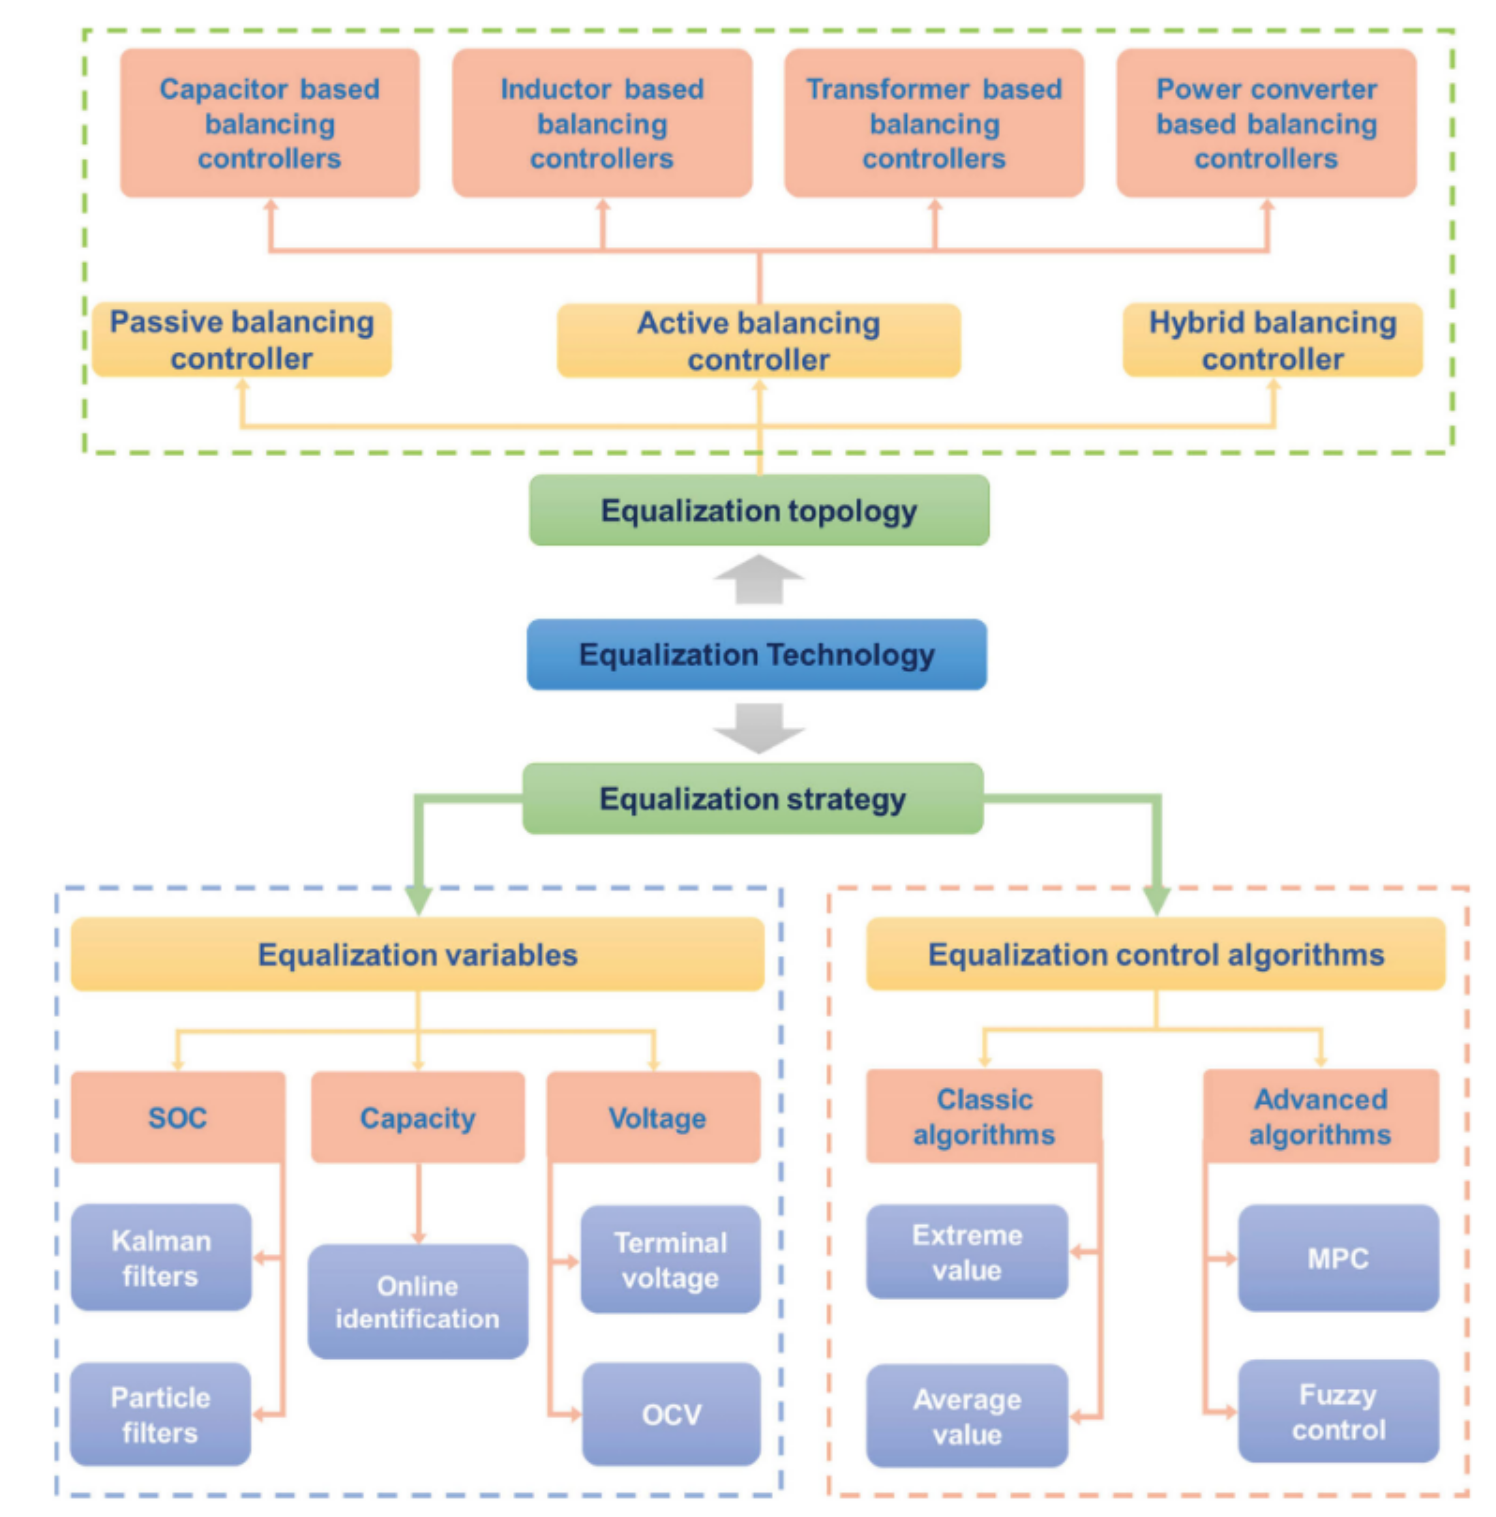
\includegraphics[width=0.75\textwidth]{ems_class.png}
        \caption{Clasificaciones t\'ipicas de los \acrshort{EMS}}
        \label{ems_classes}
    \end{center}
\end{figure}

Como se observa en la Figura \ref{passive_eq_top}, la topolog\'ia de
ecualizaci\'on pasiva generalmente emplea una resistencia en paralelo para
disipar la energ\'ia excesiva. Como se muestra en las Figuras
\ref{energy_transfer} a \ref{hier_bal_top}, las topolog\'ias activas pueden
tranferir energ\'ia entre celdas, m\'odulos y packs con la ayuda de estructuras
que no disipan energ\'ia, tales como inductores y capacitores. Ambas
topolog\'ias son beneficiosas en desacelerar la degradaci\'on de un pack de
bater\'ias extendiendo su vida \'util.

Los \acrshort{EMS} son aplicados en condiciones est\'aticas o semi-est\'aticas 
como por ejemplo, en el proceso de fin de carga, aunque investigaciones 
recientes mostraron aplicaciones de balanceo bajo condiciones din\'amicas del 
proceso de carga y descarga. En \cite{shen_cell_bal} se propone un esquema de 
ecualizaci\'on activa que comienza el trabajo una vez que la bater\'ia est\'a
completamente cargada o descargada para minimizar la transferencia de carga 
durante el proceso de balanceo.

\subsubsection{Control de balanceo pasivo}\label{seq:balanceo_pasivo}

Los controladores de balanceo pasivos (del ingl\'es
\emph{\acrfull{PBC}}) generalmente emplean resistencias \emph{shunt} en paralelo
con las bater\'ias para disipar la energ\'ia excesiva de las celdas con alto
voltaje o alto \acrshort{SOC}.

Como se muestra en la Figura \ref{passive_eq_top}A, el \acrshort{PBC} puede
controlar switches dedicados ($\mathrm{K_1}$, $\mathrm{K_2}$, ...,
$\mathrm{K_n}$), t\'ipicamente semiconductores como MOSFETs, que disipan
energ\'ia de las celdas correspondientes. Por ejemplo, asumiendo que la celda 1
tiene mayor energ\'ia que el resto, entonces el interruptor $\mathrm{K_1}$ se 
cierra para descargar esta celda. El camino de la energ\'ia es indicado por la 
línea a trazos de color azul. Dependiendo de la estrategia de ecualizaci\'on, 
los interruptores pueden funcionar continuamente o de forma intermitente, y la
energ\'ia disipada por la resistencia \emph{shunt} puede ser estimada por la
ley de Joule (\emph{Eq. \ref{joule_law}}).

\begin{equation}
    Q_{disipada} = I^2_{balanceo}R \label{joule_law}
\end{equation}

Donde $\mathrm{Q_{disipada}}$ es la potencia disipada, $\mathrm{I_{balanceo}}$
es la corriente de \emph{bypass} que circula por la resistencia \emph{shunt}, y
R es el valor de la resistencia \emph{shunt}.

La t\'ecnica \acrshort{PBC} es popular en los \acrshort{VVEE} debido a su simple
topolog\'ia y baja complejidad. Sin embargo, posee desventajas tales como la
baja eficiencia de balanceo y largos tiempos de ecualizaci\'on debido a su
limitada potencia de disipaci\'on por los componentes pasivos, limitando su
aplicaci\'on particularmente para bater\'ias de alta capacidad.

En \cite{CAMPESTRINI2016142} se estudia el balanceo pasivo tradicional de celdas 
de litio-ion usando 8 m\'odulos conectados en serie, cada uno compuesto por 14 
celdas conectadas en paralelo (8s14p). Los resultados muestran que los m\'odulos 
con \acrshort{PBC} tienen menos de 1\% de variaci\'on en capacidad despu\'es de 
1200 ciclos. Sin embargo, la celda utilizada en este estudio tiene una capacidad
nominal de 2800mAh que no es suficiente para predecir el efecto de la
ecualizaci\'on de esta t\'ecnica sobre bater\'ias de alta capacidad.

Para incrementar la corriente de balanceo, \cite{XU20192948} propone el 
desarrollo de una topolog\'ia de balanceo especial, en donde la resistencia 
shunt es reemplazada por un MOSFET, como se puede observar en la Figura
\ref{passive_eq_top}B. Por ejemplo, asumiendo que la celda 2 tiene mayor
energ\'ia que el resto, entonces el MOSFET $\mathrm{S_2}$ funciona como una
resistencia \emph{shunt} mientras que el resto permanece apagado. 

En \cite{amin_et_al_bal} se propone una topolog\'ia de balanceo pasiva que 
combina una resistencia shunt con MOSFETs. El \acrshort{PBC} fue implementado 
en un pack de 15 celdas $\mathrm{LiFePO_4}$ con una capacidad de 200Ah. Sin 
embargo, el proceso de balanceo toma mucho tiempo bajo condiciones de 
operaci\'on.

En \cite{SCHMID201749} se propone una topolog\'ia de ecualizaci\'on denominada 
\emph{balanceo electroqu\'imico} para balancear celdas sin dispositivos 
electr\'onicos adicionales que consite en conectar cada celda en serie con una 
celda de n'iquel-metal o n'iquel-zinc en paralelo. Las celdas de litio-ion pueden 
alcanzar la ecualizaci\'on con el proceso electroqu\'imico de las celdas de 
n'iquel. Los resultados verifican que este m\'etodo es posible de implementar, 
sin embargo hay una limitaci\'on de costos, volumen y complejidad muy alta.

\begin{figure}[h!]
    \begin{center}
        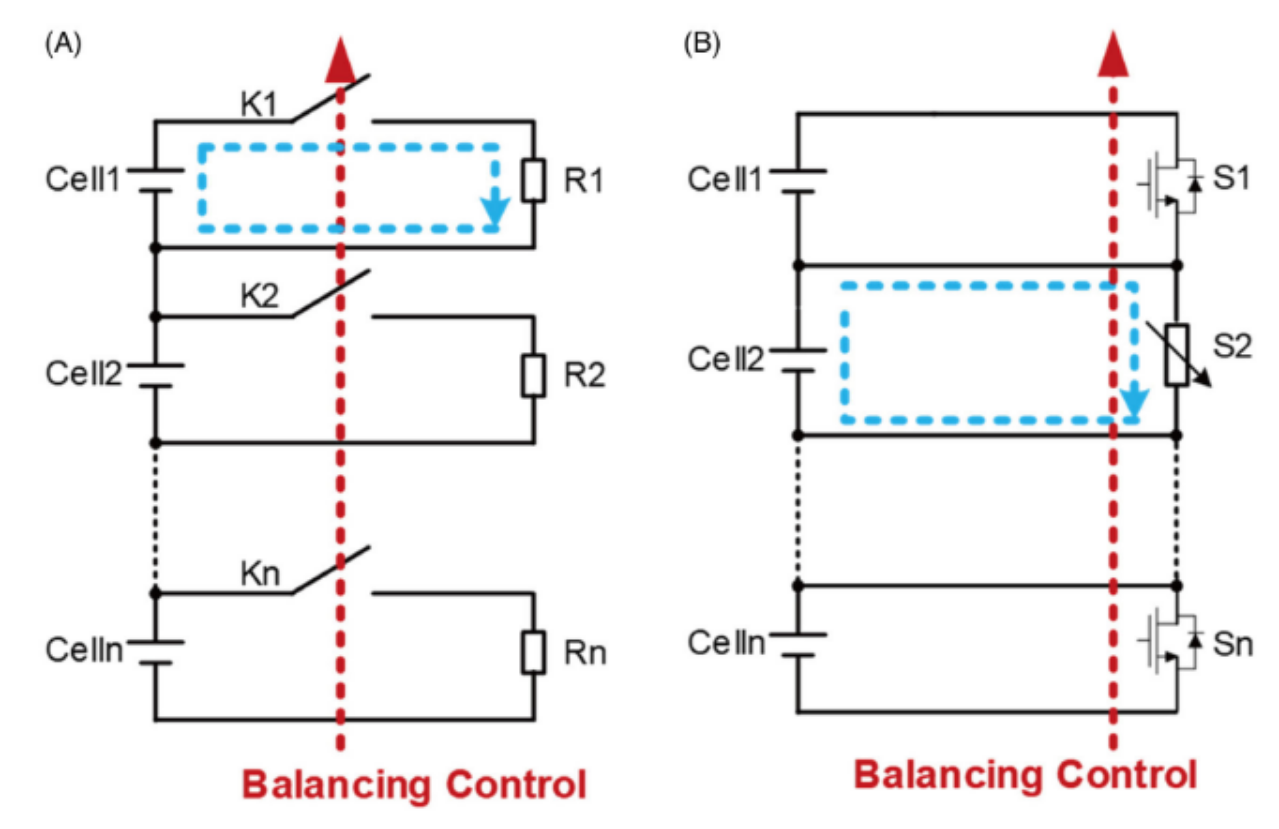
\includegraphics[width=0.75\textwidth]{passive_eq_top.png}
        \caption{Topolog\'ia de un circuito balanceador pasivo. (A) Resistencia
        tradicional con baja corriente de balanceo. (B) Topolog\'ia basada en
        MOSFET que utiliza $\mathrm{R_{DS_{on}}}$ soportando altas corrientes.}
        \label{passive_eq_top}
    \end{center}
\end{figure}

\subsubsection{Controlador de Balanceo Activo}

Los controladores de balanceo activo (\acrshort{ABC}, del ingl\'es \acrlong{ABC})
tienen topolog\'ias que, en vez de disipar energ\'ia, la transfieren entre
distintas celdas y m\'odulos/packs usando varios dispositivos que act\'uan como
\emph{buffers} de energ\'ia, incluyendo capacitores, transformadores, inductores
y convertidores de potencia.

Las principales ventajas de los \acrshort{ABC}s consiste en alta eficiencia,
alta velocidad y alta precisi\'on. Sin embargo, comparado con los 
\acrshort{PBC}s, los \acrshort{ABC}s tienen que enfrentar ciertas dificultades, 
como por ejemplo estructuras complejas, grandes tamaños y sistemas costosos de 
implementar.

\subsubsubsection{Camino de transferencia de energ\'ia}

Una de las ventajas superiores de los \acrshort{ABC}s es que la energ\'ia se
puede transferir entre distintos niveles para alcanzar un balanceo del sistema,
que reduce el consumo de energ\'ia cuando se busca lograr la ecualizaci\'on del
pack de bater\'ias. Considerando el camino de esta transferencia de energ\'ia,
los \acrshort{ABC}s pueden clasificarse en balanceo entre celda-a-celda
(\acrshort{C2C}, del ingl\'es \emph{\acrlong{C2C}}), balanceo entre
celda-a-m\'odulo (\acrshort{C2M}, del ingl\'es \emph{\acrlong{C2M}}), balanceo
entre m\'odulo-a-celda (\acrshort{M2C}, del ingl\'es \emph{\acrlong{M2C}}). La
flexibilidad en la transferencia de energ\'ia se puede observar en la Figura
\ref{energy_transfer}.

Como se observa en la Figura \ref{energy_transfer}A, la ecualizaci\'on
\acrshort{C2C} denota que la energ\'ia puede ser transferida entre las celdas de
un mismo m\'odulo/pack, que es el modo fundamental de los \acrshort{ABC}s. En
\cite{phung_bal} se presenta una arquitectura \acrshort{C2C} optimizada que se 
basa en la topolog\'ia tradicional de balanceo contiguo, que es m\'as compacto y 
f\'acil de implementar. Para n celdas conectadas en series, la arquitectura 
\acrshort{C2C} generalmente necesita n-1 componentes de transferencia de 
energ\'ia. Por lo tanto, a medida que aumenta el n\'umero de celdas conectads en
serie, el circuito se hace m\'as complicado de implementar.

Como se muestra en la Figura \ref{energy_transfer}B, la ecualizaci\'on
\acrshort{C2M} puede transferir energ\'ia entre el m\'odulo  y la celda interna
de forma bidireccional, que tiene la ventaja de desaparear la inconsistencia
entre los m\'odulos de las bater\'ias. Los autores en \cite{lu_et_al_bal} 
proponen un controlador aislado bidireccional tipo \acrshort{C2M} con una 
conmutaci\'on suave a cero voltaje. Cuando funciona en modo \emph{boost}, el 
convertidor puede transferir energ\'ia de la bater\'ia al m\'odulo, mientras que 
cuando funciona en modo \emph{buck} la transferencia de energ\'ia se realiza 
desde el m\'odulo a la celda descargada. \'Esta metodolog\'ia demuestra 
resultados experimentales con buen rendimiento tanto en velocidad como 
eficiencia.

La Figura \ref{energy_transfer}C muestra una arquitectura \acrshort{M2M}
donde la transferencia de energ\'ia se realiza entre m\'odulos. Comparado con
las arquitecturas \acrshort{C2C} y \acrshort{C2M}, la arquitectura 
\acrshort{M2M} generalmente tiene un tamaño considerablemente grande teniendo en 
cuenta la aislaci\'on de corriente y una estrategia compleja para evitar el 
desbalanceo, haciendo que esta implementaci\'on sea m\'as dificultosa que el 
resto. En \cite{ji_et_al_bal_mod} se propone un esquema de ecualizaci\'on usando 
m\'ultiples transformadores que con permiten que la energ\'ia pueda ser 
transferida entre m\'odulos de distintos voltajes, alcanzado una corriente de 
balanceo de hasta 3A mientras que la inconsistencia entre voltajes es de 24mV.

Otros m\'etodos no ilustrados en la Figura \ref{energy_transfer} tambi\'en
fueron estudiados. Por ejemplo, en \cite{li_et_al_bal} se propone una 
topolog\'ia de ecualizaci\'on m\'odulo-a-celda-a-m\'odulo. Con la ayuda de 
conmutaci\'on suave a cero voltaje y un circuito bidireccional resonante, la 
velocidad y eficiencia del m\'etodo puede ser mejorado de forma considerable. 
Los resultados experimentales muestran que la topolog\'ia puede obtener una 
eficacia del 93\% en modo \acrshort{C2M} y 72.5\% en modo \acrshort{M2C}.

\begin{figure}[h!]
    \begin{center}
        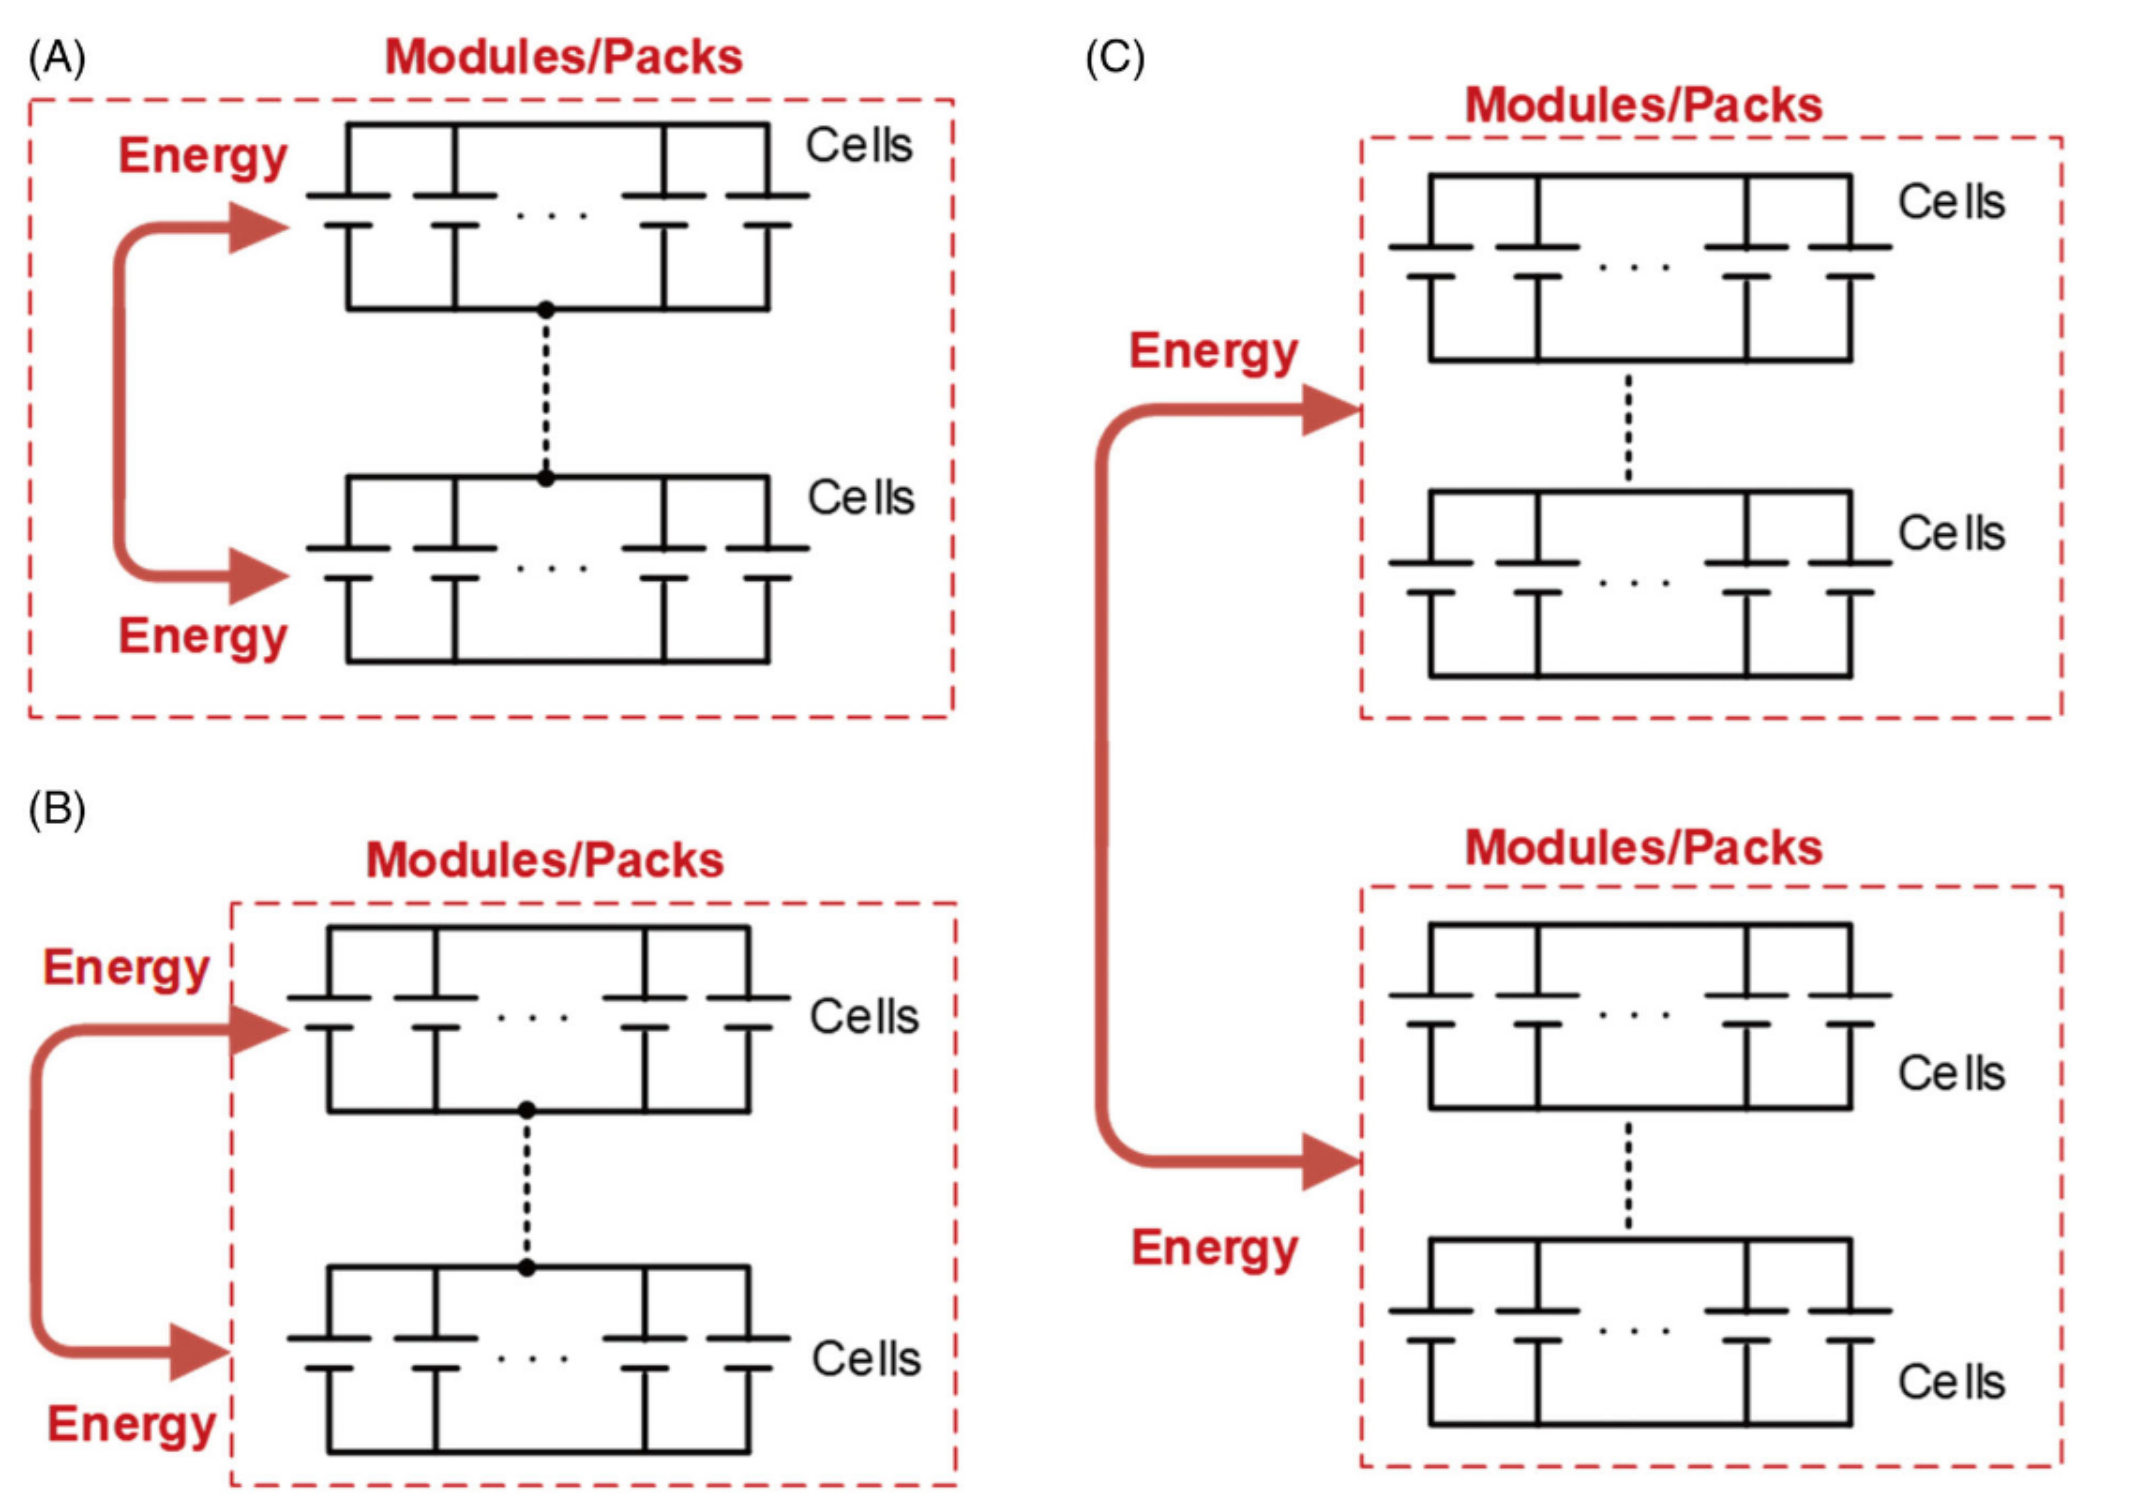
\includegraphics[width=0.8\textwidth]{energy_transfer.png}
        \caption{Diferentes caminos de transferencia de energ\'ia. (A)
        Celda-A-Celdas (\acrshort{C2C}). (B) Celda-A-M\'odulo (\acrshort{C2M}).
        (C) M\'odulo-A-M\'odulo (\acrshort{M2M})} 
        \label{energy_transfer}
    \end{center}
\end{figure}

\subsubsubsection{Controlador de balanceo basado en capacitores}

Los controladores de balanceo basados en capacitores (\acrshort{CBBC}, del
ingl\'es \emph{\acrlong{CBBC}}) pueden transportar energ\'ia entre celdas o
entre celdas, m\'odulos y sistemas.

Como se muestra en la Figura \ref{cbbc_top}, los \acrshort{CBBC}s pueden ser 
clasificados en una topolog\'ia de un solo capacitor, capacitor alternado y una 
topolog\'ia de capacitores multi-capa. Los \acrshort{CBBC} solo pueden 
transferir energ\'ia entre bater\'ias que poseen un voltaje de diferencia 
significativo.

Una t\'ipica topolog\'ia de un solo capacitor se puede observar en la Figura
\ref{cbbc_top}A, que adem\'as de poseer un solo capacitor (C), est\'a compuesto
de varios interruptores unipolares (\acrshort{SPST}, del ingl\'es 
\emph{\acrlong{SPST}}) y bipolares (\acrshort{SPDT}, del ing\'es 
\emph{\acrlong{SPDT}}). 

La topolog\'ia \acrshort{CBBC} con un solo capacitor, con una estrategia de
control muy simple y baja p\'erdida de energ\'ia, tiene la desventaja de que el
tiempo de balanceo es extenso. Durante la operaci\'on, el ecualizador detecta
las celdas con mayores y menores voltajes, y despu\'es realiza la transferencia
de energ\'ia entre las celdas seleccionados con el control de los
\acrshort{SPST}. El proceso de ecualizaci\'on comienza con la carga del
capacitor por la bater\'ia de alto voltaje y contin\'ua con la descarga del
capacitor en la celda de bajo voltaje. Por ejemplo, asumiendo que la celda 1 y
la celda 2 son las celdas con el mayor y el menor voltaje respectivamente,
inicialmente, los \acrshort{SPST} $\mathrm{K_1}$ y $\mathrm{K_2}$ son conectados
con el lado de bajo voltaje y los \acrshort{SPDT} $\mathrm{S_1}$ y 
$\mathrm{S_2}$ son conectados al lado de alto voltaje, provocando la
transferencia de la energ\'ia desde la celda 1 al capacitor C como se muestra en
la línea azul. Una vez cargado el capacitor, $\mathrm{K_1}$ es desconectado,
mientras que $\mathrm{K_2}$ y $\mathrm{K_3}$ se cierran, por el otro lado
$\mathrm{S_1}$ y $\mathrm{S_2}$ son conectados al lado bajo y la energ\'ia
ser\'a transferida desde el buffer hasta la celda 2 como se muestra en la línea
verde.

Una topolog\'ia t\'ipica de un capacitor alternado se muestra en la Figura
\ref{cbbc_top}B, que consiste de varios capacitores y \acrshort{SPDT}s para
transmitir energ\'ia entre bater\'ias contiguas con el control de los
interruptores. Los \acrshort{CBBC}s con esta toplog\'ia tienen ventajas 
similares a la estructura de un solo capacitor, como por ejemplo, una estructura 
simple y de bajo costo, pero requiere de una estrategia de control finamente 
ajustada, especialmente cuando hay una pequeña diferencia de voltaje entre las 
celdas adyacentes. Las líneas azul y verde muestran como es el camino de 
transferencia de la energ\'ia.

La Figura \ref{cbbc_top}C muestra una topolog\'ia de capacitores de dos capas
que transfiere energ\'ia entre celdas adyacentes a trav\'es de la primer capa y
transfiere energ\'ia entre las bater\'ias que no est\'an conectadas de forma
directa a trav\'es de la segunda capa, reduciendo significativamente el tiempo
de ecualizaci\'on. La línea azul muestra la transferencia de energ\'ia entre la
celda 1 y la celda 2 a un capacitor de la segunda capa ($\mathrm{C_{21}}$), y la
energ\'ia puede ser transferida desde $\mathrm{C_{21}}$ a la celda 2 y 3 para
lograr la transmisi\'on de la celda 1 a la 3 como se muestra en la línea verde. 

Una topolog\'ia t\'ipica multicapa se puede observar en la Figura
\ref{cbbc_top}D. Adem\'as de la transferencia entre celdas del mismo m\'odulo,
esta topolog\'ia nos permite transmitir energ\'ia entre m\'odulos. 

Por \'ultimo, a pesar de las t\'ipicas estructuras todav\'ia se encuentran
en desarrollo e investigaci\'on nuevas tecnolog\'ias basadas en capacitores,
como por ejemplo, en \cite{shang_et_al_bal_cap} se propone un ecualizador de 
capacitores basados en una estructura de tipo malla (del ingl\'es \emph{mesh}) 
que mejora de manera significativa la eficiencia y velocidad del balanceo. 
Su estructura se puede observar en la Figura \ref{cbbc_mesh_top}

\begin{figure}[h!]
    \begin{center}
        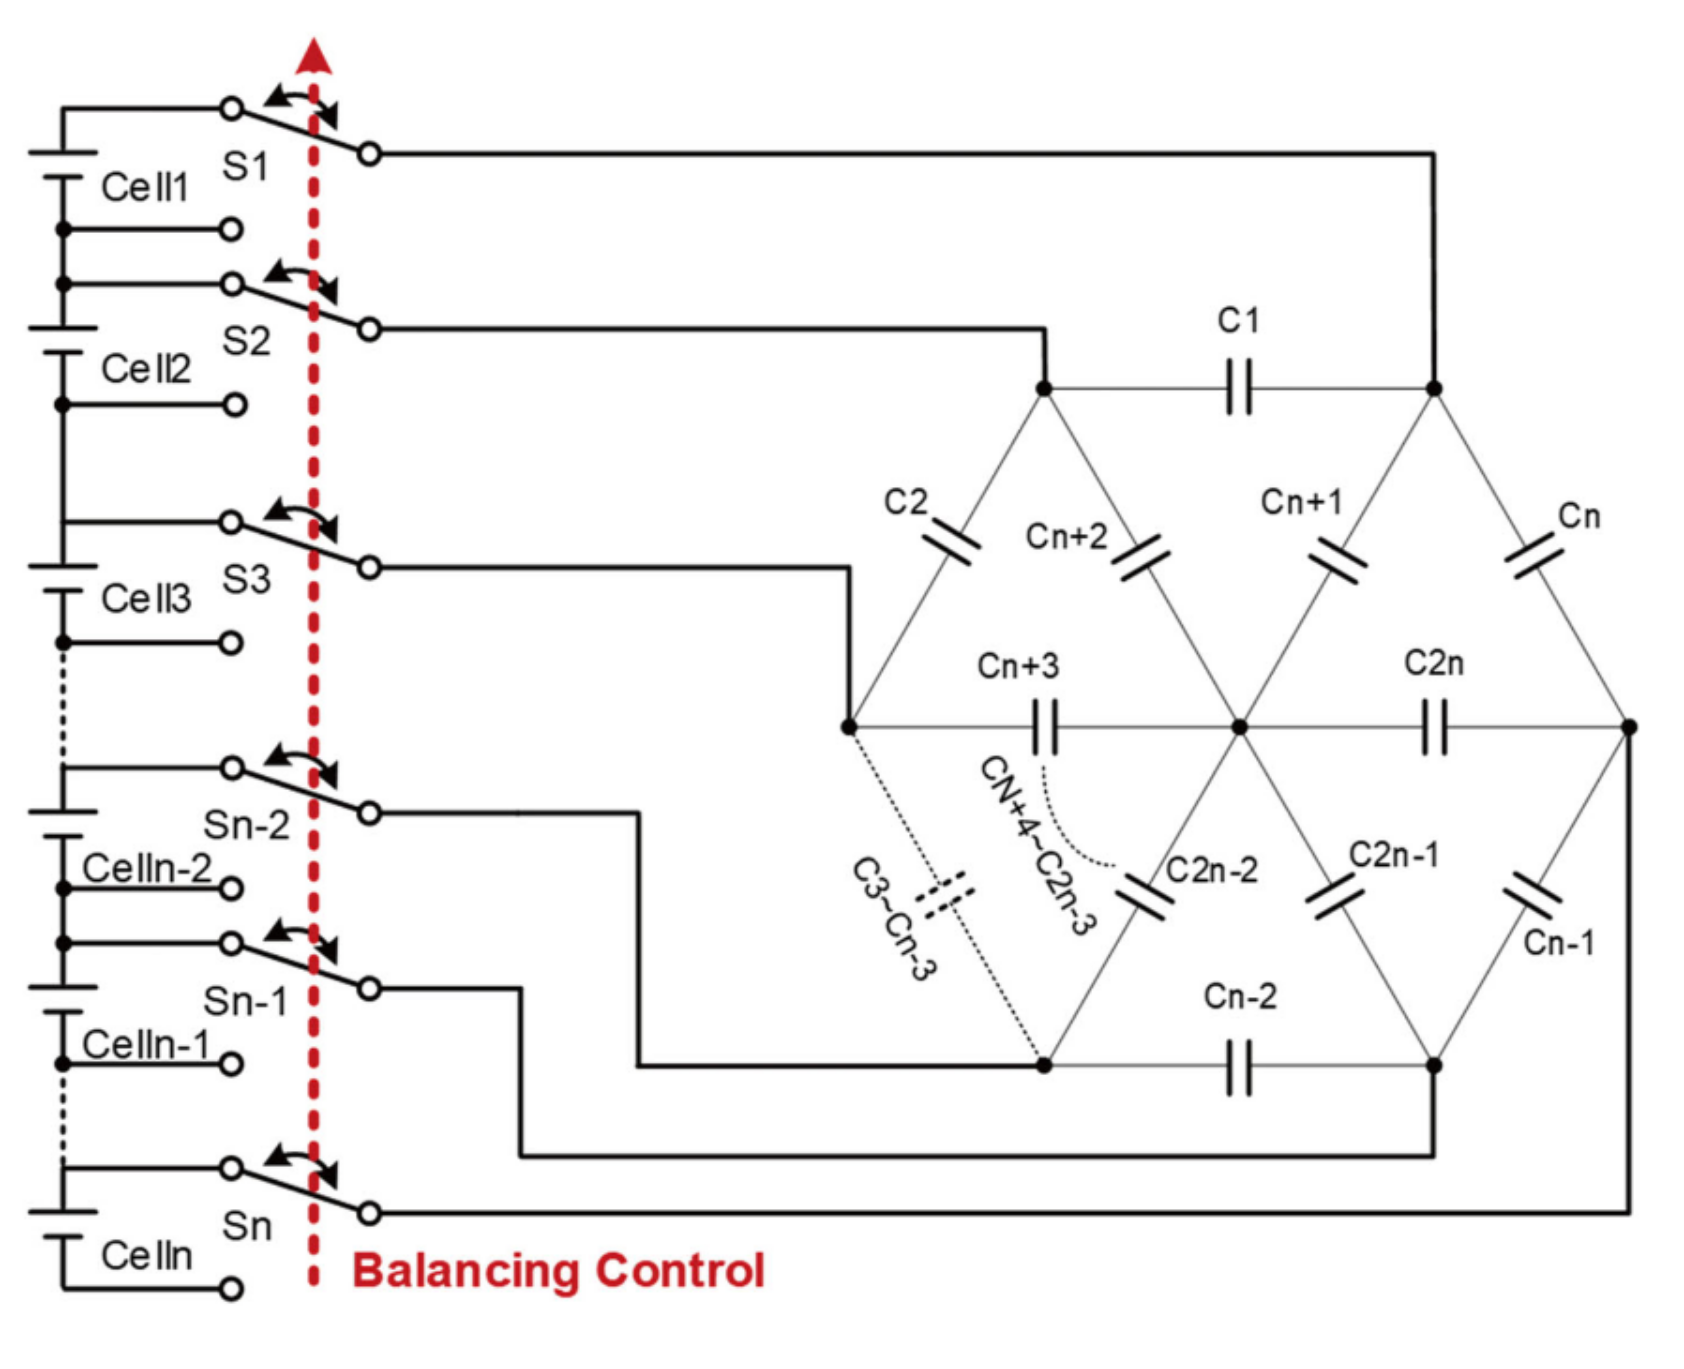
\includegraphics[width=0.7\textwidth]{cbbc_mesh_top.png}
        \caption{Balanceador de celdas basado en capacitores con una topolog\'ia
        de tipo red.}
        \label{cbbc_mesh_top}
    \end{center}
\end{figure}

\begin{figure}[h!]
    \begin{center}
        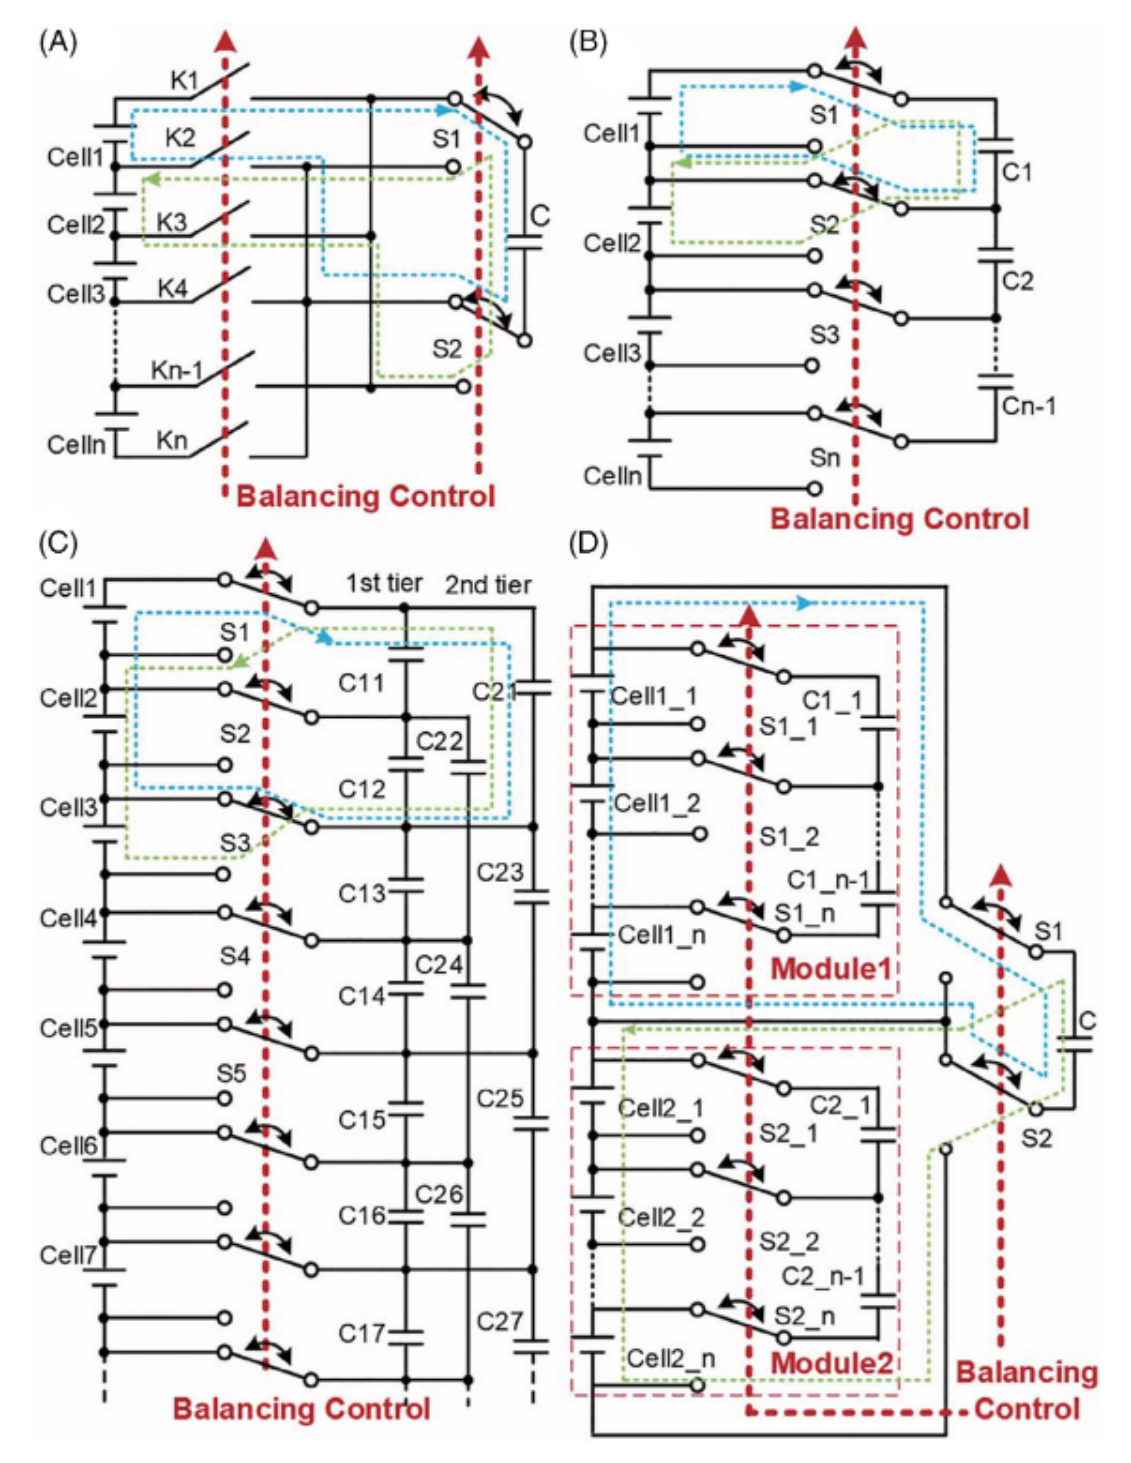
\includegraphics[width=0.8\textwidth]{cbbc_top.png}
        \caption{Topolog\'ias de balanceo basada en capacitores. (A) Topolog\'ia
        de capacitor simple (\acrshort{C2C}). (B). Topolog\'ia de capacitores
        alternantes (\acrshort{C2C}). (C) Topolog\'ia basada en dos capas de
        capacitores (\acrshort{C2C}). (D) Topolog\'ia de capacitores multi-capa
        (\acrshort{C2C})}
        \label{cbbc_top}
    \end{center}
\end{figure}

%\newpage

\subsubsubsection{Controlador de balanceo basado en inductores}

Los controladores de balanceo basado en inductores (\acrshort{IBBC}, del
ingl\'es \acrlong{IBBC}) pueden transferir energ\'ia entre celdas y m\'odulos a
trav\'es de inductores externos. Comparado con los \acrshort{CBBC}s, los
\acrshort{IBBC}s t\'ipicamente est\'an relacionados con velocidades de balanceo
m\'as r\'apidas debido a una corriente de ecualizaci\'on m\'as alta, sin embargo
\acrshort{IBBC}s son generalmente m\'as costosos y menos eficientes.

Los \acrshort{IBBC}s pueden ser clasificado entre distintas topolog\'ias, como por
ejemplo, una topolog\'ia de un inductor simple o inductores alternativos, como
se observa en la Figura \ref{ibbc_top}.

\begin{figure}[h!]
    \begin{center}
        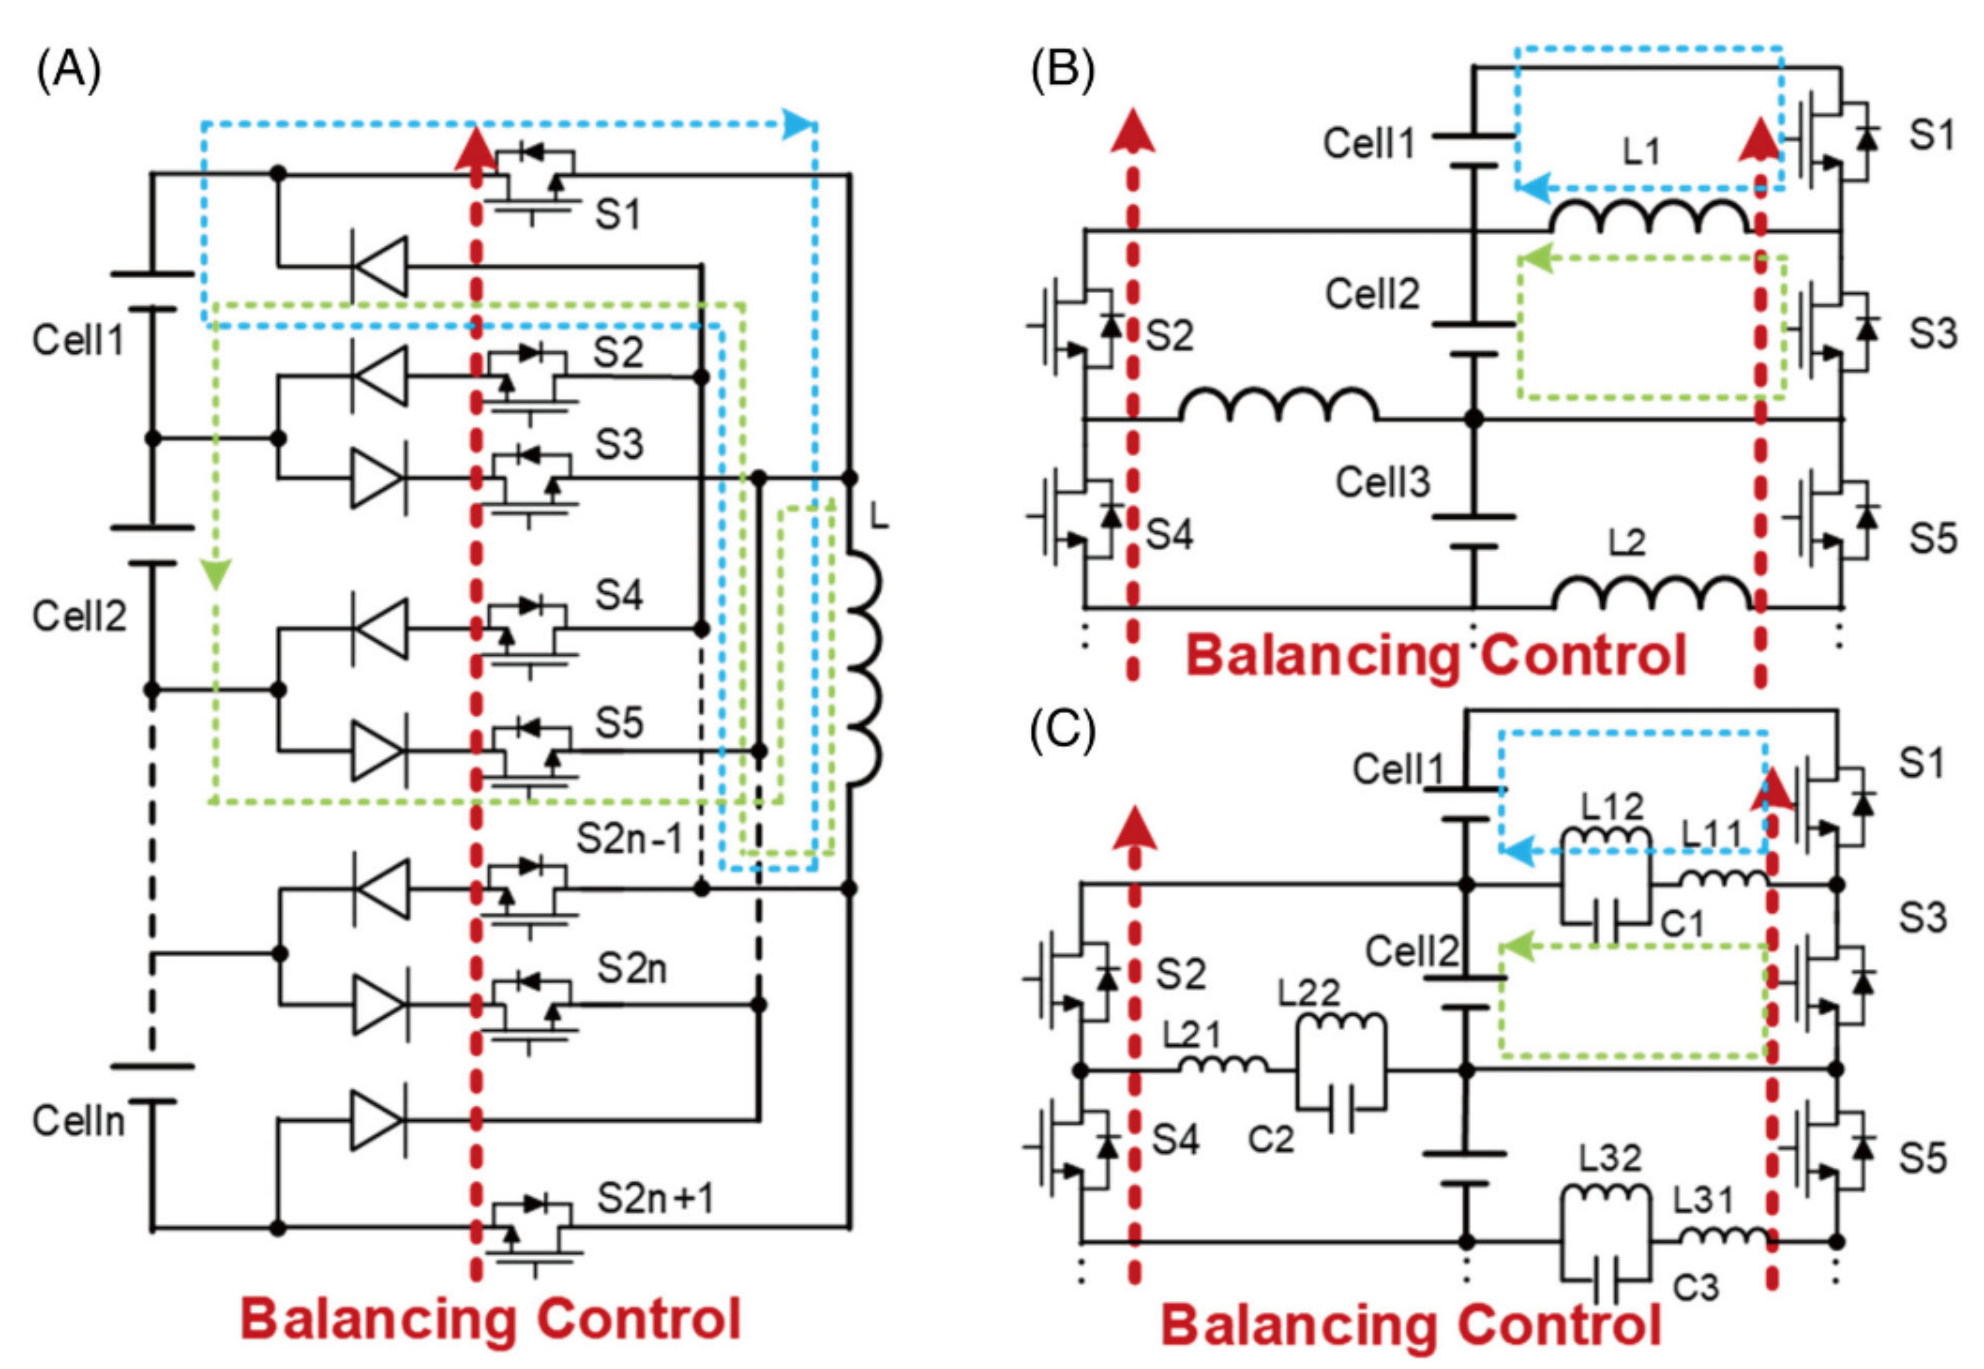
\includegraphics[width=0.8\textwidth]{ibbc_top.png}
        \caption{topolog\'ias de balanceo basadas en inductores. (A) Topolog\'ia
        de inductor simple (\acrshort{C2C}). (B) Topolog\'ia de m\'ultiples
        inductores (\acrshort{C2C}). (C) Topolog\'ia de inductores resonantes
        (\acrshort{C2C})}
        \label{ibbc_top}
    \end{center}
\end{figure}

Una topolog\'ia t\'ipica de inductor simple se puede observar en la
Figura\ref{ibbc_top}A, que incluye un solo inductor y varios MOSFETs que permite
transferir la energ\'ia entre celdas seleccionadas controlando los MOSFETs con
señales \acrshort{PWM} (del ingl\'es \emph{\acrlong{PWM}}). Por ejemplo, 
asumiendo que la celda 1 y 2 son las celdas con mayor y menor voltaje 
respectivamente. Los MOSFETs S1 y S2 son inicialmente encendidos, permitiendo 
que la energ\'ia se transfiera de la celda 1 a la inductancia L, como muestra la 
línea azul. La energ\'ia transferida se puede calcular con la Ecuaci\'on 
\ref{energy_trans_ind}:

\begin{equation}
    \dot{Q} = UI = IL\frac{dI}{dt} \label{energy_trans_ind}
\end{equation}

donde L es el valor de la inductancia, U e I son la tensi\'on de los terminales
de la bater\'ia y la corriente que circula por el inductor respectivamente.
Entonces cuando el interruptor S1 se apaga y se enciende S5, la energ\'ia se
transfiere desde la inductancia a la celda 2 como muestra la línea verde.
Las señales \acrshort{PWM} son utilizadas como señales de control que comandan 
los MOSFETs para transferir energ\'ia entre las celdas.

Una configuraci\'on t\'ipica de m\'ultiples inductores se puede observar en la
Figura \ref{ibbc_top}B, que consiste de varios inductores y MOSFETs. La
energ\'ia transferida entre celdas es, nuevamente, controlada por los MOSFETs. 
Las líneas azules y verdes muestran los caminos de transferencia de 
energ\'ia para la descarga de la celda 1 y la carga de la celda 2. La velocidad 
de ecualizaci\'on para tales topolog\'ias se encuentra afectada por la escala 
del pack, y la velocidad es generalmente baja porque la transferencia de 
energ\'ia solo se puede realizar entre celdas adyacentes.

En la Figura \ref{ibbc_top}C se muestra un circuito de inductor resonante. Este
circuito es utilizado como reemplazo del inductor simple, debido a que puede
reducir la interferencia electromagn\'etica (\acrshort{EMI}, del ingl\'es
\emph{\acrlong{EMI}}) e incrementar las p\'erdidas provocadas por la
conmutaci\'on durante el proceso de ecualizaci\'on. Las líneas azul y verde
muestran el intercambio de energ\'ia para la descarga de la celda 1 y la carga
de la celda 2 respectivamente.

%Note: (FDC) No logro ver como podríamos pasar energía con una inductancia desde
%una delda de menor voltaje a una de mayor

%Una caracter\'istica particular de los circuitos \acrshort{IBBC}s es que la
%transferencia de energ\'ia se puede hacer desde una celda con menor voltaje a
%una celda de mayor voltaje. Por lo tanto, la estrategia de balanceo debe ser
%considerada cuidadosamente para evitar un error de balanceo.

\subsubsubsection{Controlador de balanceo basado en transformadores}

Los controladores de balanceo basados en transformadores (\acrshort{TBBC}, del
ingl\'es \emph{\acrlong{TBBC}}) pueden transferir energ\'ia entre distintas celdas y
m\'odulos a trav\'es de transformadores externos. Como se muestra en la Figura
\ref{tbbc_top}, los \acrshort{TBBC} se pueden dividr en transformadores de
devanado simple o transformadores de m\'ultiples devanados.

\begin{figure}[h!]
    \begin{center}
        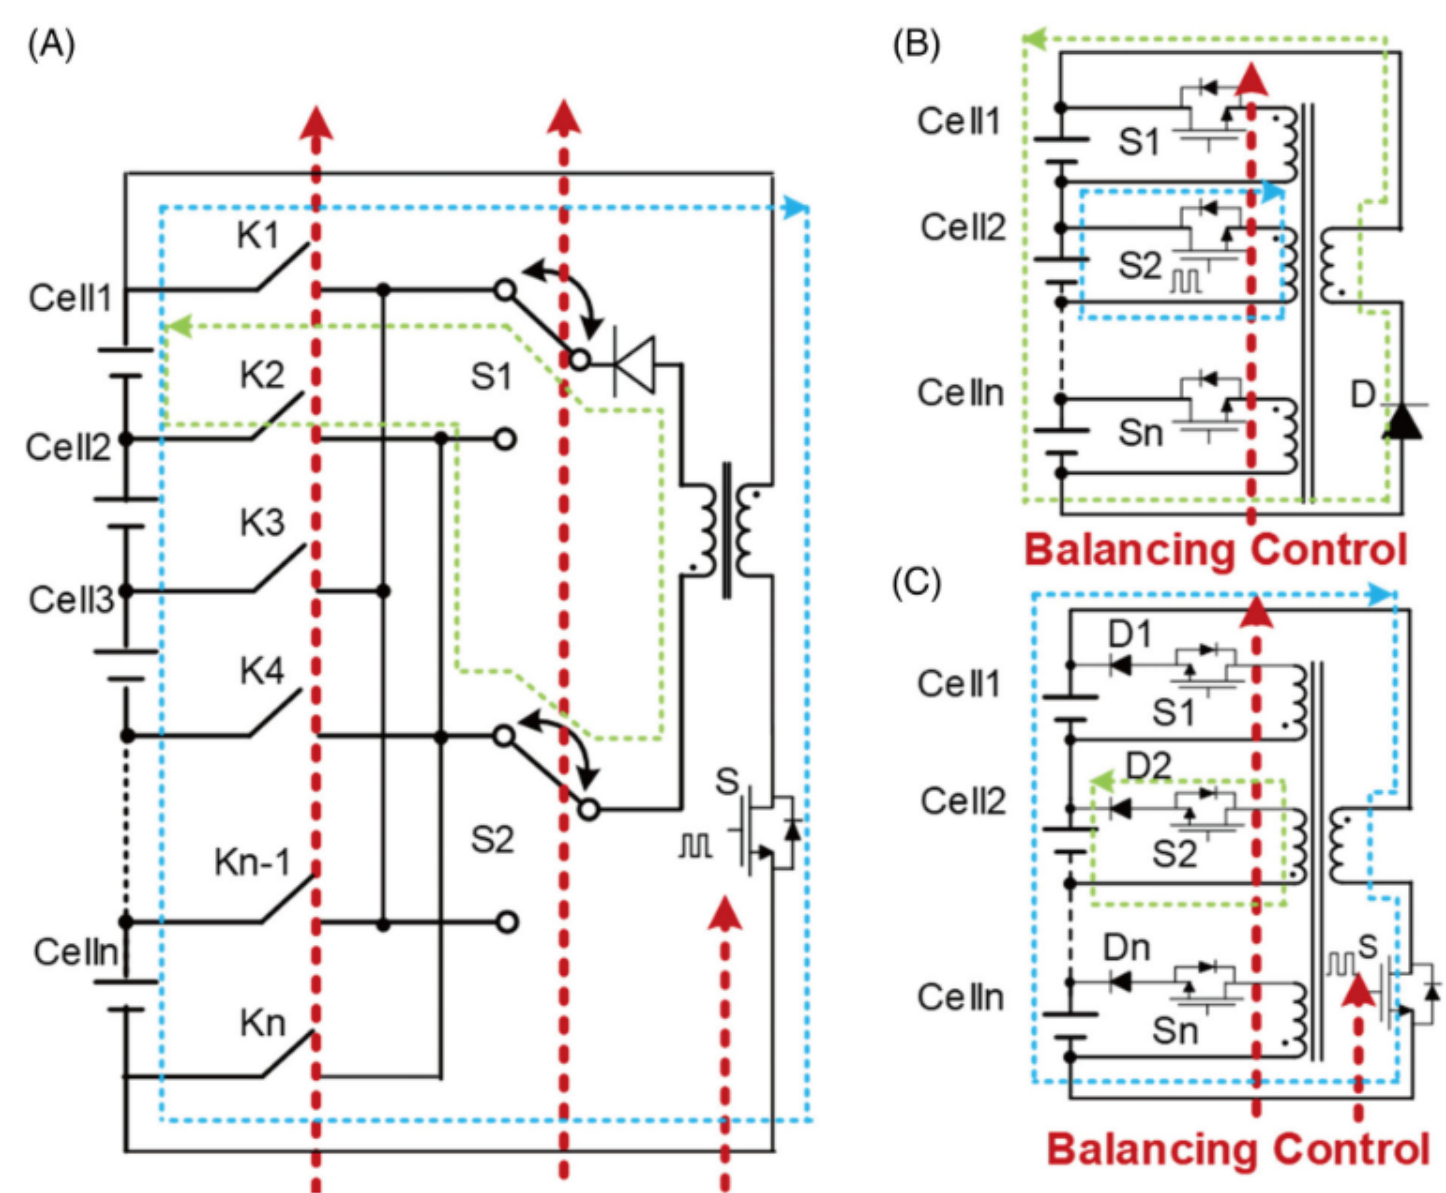
\includegraphics[width=0.75\textwidth]{tbbc_top.png}
        \caption{Topolog\'ias de balanceo basados en transformadores. (A)
        topolog\'ia basada en un transformador de devanado simple
        (\acrshort{M2C}). (B) Topolog\'ia de tranformadores de devanados
        m\'ultiples (\acrshort{C2M}). (C) Topolog\'ia de transformadores de
        devanados m\'ultiples (\acrshort{M2C})}
        \label{tbbc_top}
    \end{center}
\end{figure}

En la Figura \ref{tbbc_top}A se puede observar una topolog\'ia \acrshort{TBBC}
basada en un transformador de devanado simple, que puede transferir energ\'ia de
forma \acrshort{M2C} controlando los interruptores del circuito. Por ejemplo,
asumiendo que la celda 1 es la celda con la mejor energ\'ia. Inicialmente, el
MOSFET S se cierra y comienza a circular corriente desde el m\'odulo hacia el
transformador. La línea azul muestra el camino de esta transferencia de
energ\'ia. Una vez que el MOSFET S se apaga, los interruptores S1 y S2 son
conectados a la parte alta y baja de la celda 1 respectivamente, y la energ\'ia
almacenada en el transformador es transferida a la misma. La línea verde muestra
como se transfiere la energ\'ia desde el transformador a la celda 1. Una primer
desventaja para este tipo de topolog\'ia, que se puede observar a simple vista,
es que se necesitan transformadores de alto voltaje lo que implica un costo alto
y un gran tamaño para ser implementado, sin contar el peso, característica
fundamental a tener en cuenta en los vehículos eléctricos.

Una topolog\'ia de m\'ultiples devanados para una transferencia de energ\'ia
\acrshort{C2M} se puede observar en la Figura \ref{tbbc_top}B. Por ejemplo,
asumiendo que la celda 2 es la celda con mayor energ\'ia, el MOSFET S2 se
enciende y la corriente comienza a circular hacia el transformador en el sentido
directo. Una vez que el MOSFET S2 se apaga, la energ\'ia almacenada en el
transformador ser\'a transferida al m\'odulo. Las líneas azul y verde muestran
los caminos de esta transferencia de energ\'ia.

Por el otro lado, en la Figura \ref{tbbc_top}C se muestra una topolog\'ia basada
en transformadores de m\'ultiples devanados para una transferencia tipo
\acrshort{M2C}. Por ejemplo, asumiendo que la celda 2 es la bater\'ia con menor 
energ\'ia en el pack. Inicialmente, el MOSFET S se enciende y la corriente 
comienza a circular hacia el transformador. Una vez que el MOSFET S se apaga, el
MOSFET S2 se enciende y la energ\'ia almacenada es transferida a la celda 2. Las
señales de \acrshort{PWM} son utilizadas para regular la transferencia de
energ\'ia entre las celdas.

La velocidad de ecualizaci\'on de los \acrshort{TBBC}s son generalmente
r\'apidas, pero los voltajes en el devanado secundario son inconsistentes debido
a p\'erdidas de inductancia en el devanado de los transformadores. Otro gran
problema de estas topolog\'ias es que la fabricaci\'on de devanados sim\'etricos
para aplicaciones de alta potencia son costosos.

\subsubsubsection{Balanceadores basados en convertidores de potencia}

Los convertidores DC/DC, o convertidores de potencia, pueden convertir una fuente
DC de un voltaje a otro distinto. Los controladores de balanceo basados en
convertidores de potencia (\acrshort{PBBC}, del ing\'es \acrlong{PBBC}) tienen
la ventaja de ser altamente eficientes y precisos para la transformaci\'on de
energ\'ia de forma bidireccional. Los \acrshort{PBBC}s pueden transferir la
energ\'ia entre distintas celdas y m\'odulos. Los convertidores de potencia
aplicados en estas topolog\'ias pueden funcionar en modo reductor (del ingl\'es
\emph{buck}), elevador (del ingl\'es \emph{boost}), elevador-reductor, Cuk y
otros tipos. Ya que los convertidores de potencia DC/DC usan inductores o
transformadores como componentes de almacenamiento de energ\'ia, los
\acrshort{PBBC}s tienen algunas similitudes con los \acrshort{IBBC}s e
\acrshort{TBBC}s. Los \acrshort{PBBC}s pueden alcanzar un control muy preciso en 
el proceso de ecualizaci\'on pero con la contraparte de ser costosos y complejos 
de implementar.

El convertidor de potencia reductor disminuye el voltaje de entrada con al menos
dos semiconductores y un inductor. Una topolog\'ia de ecualizaci\'on basada en
un convertidor reductor se puede observar en la Figura \ref{pbbc_top}A. Durante
el proceso de carga, cada circuito reductor puede servir como un circuito de
carga y controlar la corriente de este proceso para cada celda de forma 
independiente. Asumiendo que el circuito reductor funciona en modo de 
conducci\'on continua, el voltaje de cada celda conectada en serie se puede 
expresar en la Ecuaci\'on \ref{pbbc_reduc_voltaje},

\begin{equation}
    V_{mi} = V_{ci} \times D_i \label{pbbc_reduc_voltaje}
\end{equation}

donde $\mathrm{V_{mi}}$ es el voltaje promedio en la i-\'esima celda,
$\mathrm{V_{ci}}$ es el voltaje promedio del capacitor correspondiente, y
$\mathrm{D_i}$ es el ciclo de trabajo de la señal de \acrshort{PWM}. Debido a
que cada m\'odulo trabaja de forma independiente, es posible alcanzar una
ecualizaci\'on del pack en corto tiempo.

Los convertidores de potencia elevadores aumentan la tensi\'on de entrada con
al menos dos semiconductores y un elemento de almacenamiento de energ\'ia. El
esquem\'atico de un circuito de balanceo basado en convertidores elevadores se
puede observar en la Figura \ref{pbbc_top}B. La corriente promedio de todos los
circuitos elevadores son iguales, pero cada corriente individual difiere
dependiendo del voltaje del m\'odulo y el ciclo de trabajo de la señal de
\acrshort{PWM} para alcanzar la ecualizaci\'on.

Los convertidores reductores-elevadores pueden implementar funciones de ambas
topolog\'ias, y el voltaje de salida puede ser mayor o menor al de entrada. Una
topolog\'ia t\'ipica que implementa estos convertidores se puede observar en
\ref{pbbc_top}C, que permite transferir energ\'ia entre bater\'ias adyacentes a
trav\'es del control de los interruptores. Por ejemplo, asumiendo que la
energ\'ia debe ser transferied desde la celda 2 a la celda 1. Inicialmente, el
MOSFET S3 se enciende y la corriente comienza a circular hacia la inductancia
L1. Una vez que el MOSFET S3 se apaga, la energ\'ia es transferida a la celda 1
a trav\'es del diodo de S1. Las señales \acrshort{PWM} son utilizadas para
controlar la transferencia de energ\'ia entre celdas a trav\'es de los MOSFETs.
Esta topolog\'ia bidireccional es ideal para las aplicaciones de balanceo debido
a su eficiencia y conveniencia. Sin embargo, nuevamente son costosos y complejos
de implementar, por lo que solo rinden para bater\'ias a gran escala y con
grandes capacidades. Por ejemplo, \cite{shang_et_al_bal_rect} introdujo la 
investigaci\'on de convertidores reductores-elevadores junto a sus resultados 
experimentales.
%\newpage
Los convertidores Cuk aumentan o disminuyen y, a la vez, invierten la tensi\'on
de entrada. Un convertidor de tipo Cuk implementado en un balanceador se puede
observar en la Figura \ref{pbbc_top}D, que contiene dos inductores y dos
MOSFETs. Durante el proceso de ecualizaci\'on, la energ\'ia puede ser
transferida entre bater\'ias contiguas con MOSFETs controlados por señales
\acrshort{PWM}, los capacitores sirven como almacenadores principales para la
transferencia de energ\'ia. Comparado con la topolog\'ia elevador-reductor, los
circuitos Cuk tienen un bajo riple y alta eficiencia, sin embargo, los mismos
contienen m\'as elementos resultando en una implementaci\'on m\'as costosa.

Finalmente, los convertidores tipo \emph{flyback} tambi\'en fueron implementados
en topolog\'ias de balanceadores basados en convertidores de potencia. En
\cite{lin_et_al_bal_bid} se propone una topolog\'ia bidireccional, basada en 
estos tipos de convertidores, que puede transferir energ\'ia entre la bater\'ia y 
un capacitor, que actua como almacenador de energ\'ia. Los resultados 
experimentales demuestran su factibilidad sobre bater\'ias de tipo 
LiFeP$\mathrm{O_4}$ adoptando una modalidad de transferencia entre m\'odulos 
(\acrshort{M2M}).

\begin{figure}[h!]
    \begin{center}
        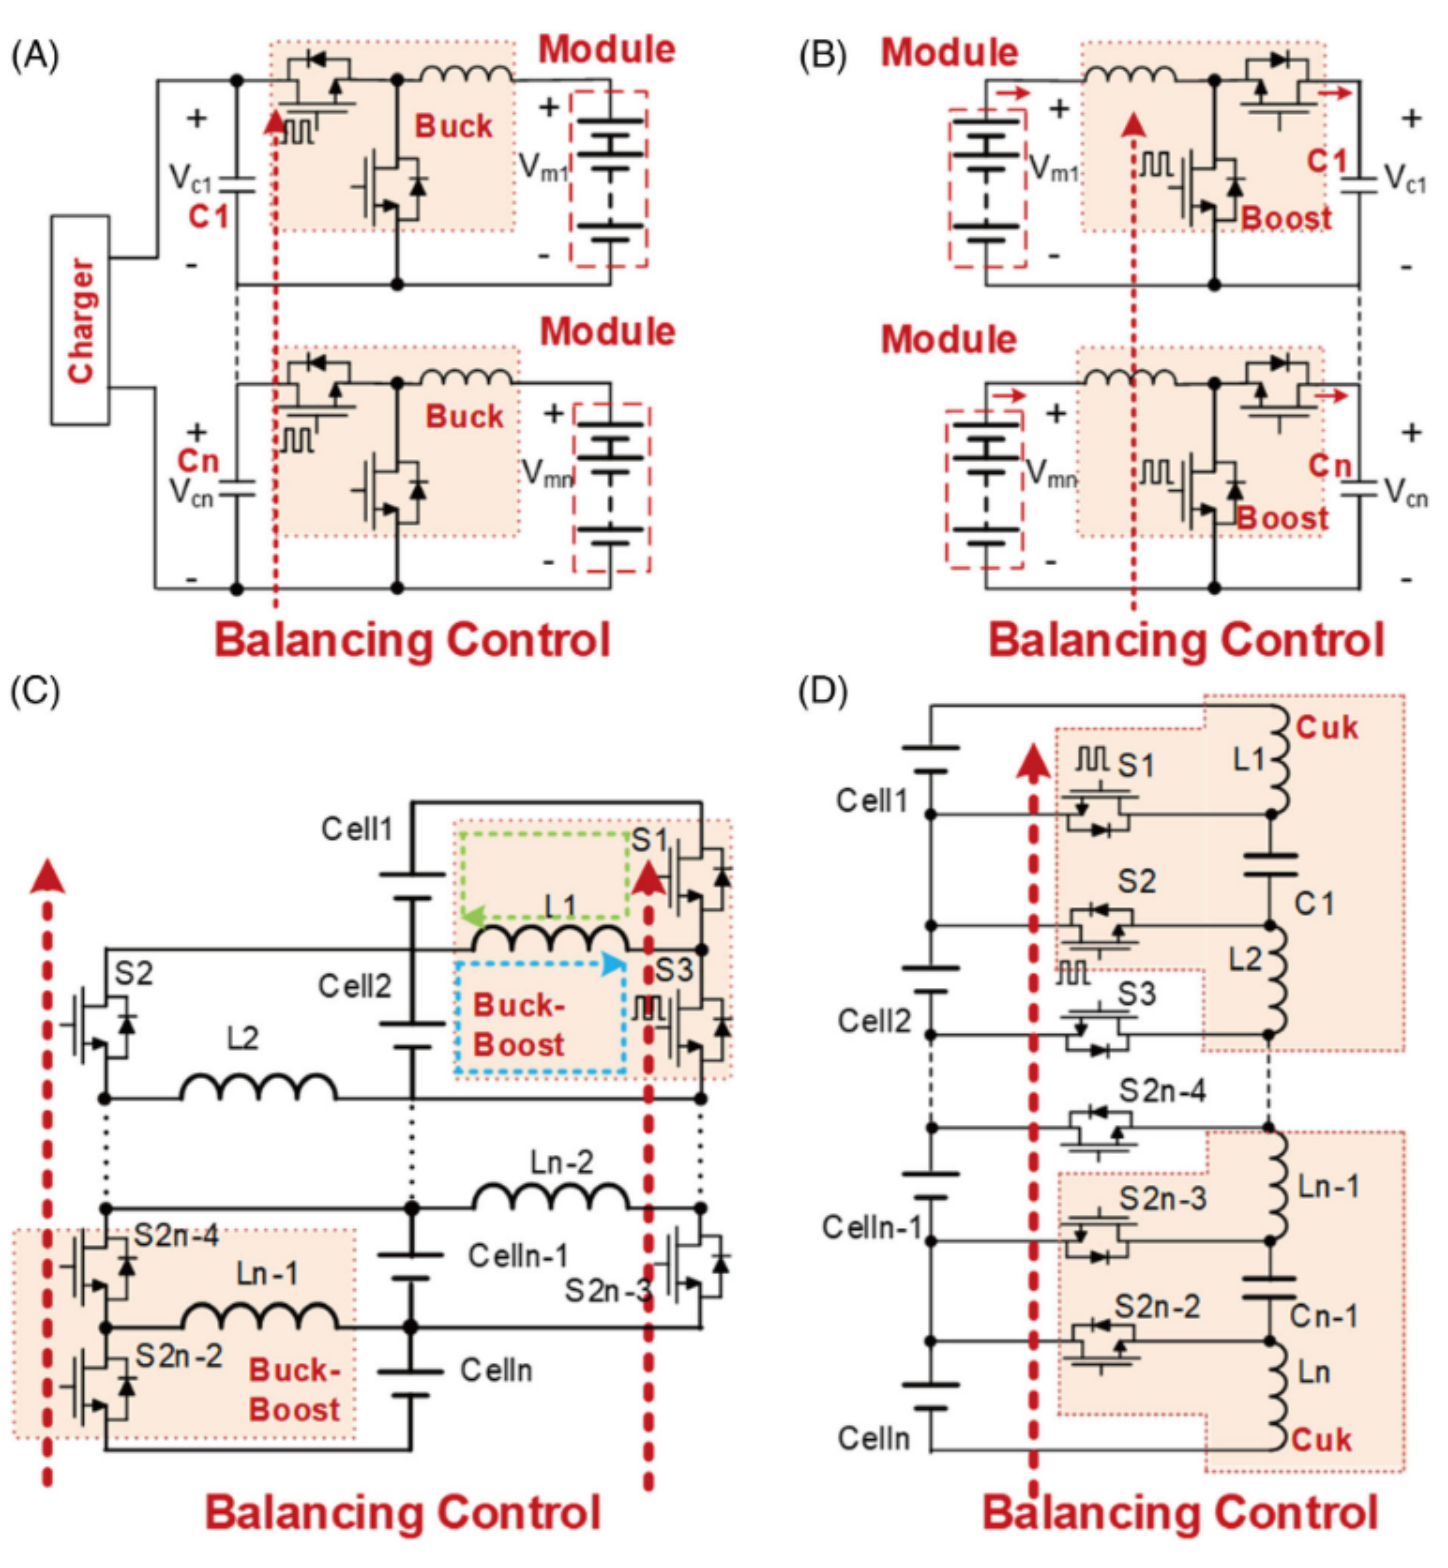
\includegraphics[width=0.8\textwidth]{pbbc_top.png}
        \caption{Topolog\'ias de balanceo basadas en convertidores de potencia.
                 (A) Topolog\'ia de ecualizaci\'on basadas en convertidores
                 reductores. (B) Topolog\'ia de ecualizaci\'on basadas en
                 convertidores elevadores. (C) Topolog\'ia de ecualizaci\'on
                 basada en una topolog\'ia reductor-elevador (\acrshort{C2C}).
                 (D) Topolog\'ia Cuk (\acrshort{C2C}).}
         \label{pbbc_top}
    \end{center}
\end{figure}
\FloatBarrier

%\newpage

\subsubsection{Topolog\'ias h\'ibridas}

Las topolog\'ias h\'ibridas pueden mejorar el rendimiento del balanceador
gracias a la combinaci\'on de una ecualizaci\'on pasiva con una activa. 
Los autores en \cite{fang_bal} proponen una topolog\'ia h\'ibrida basada en 
convertidores de potencia y resistencias \emph{shunt}. El convertidor de 
potencia puede transferir energ\'ia del m\'odulo para cargar las bater\'ias con 
un voltaje bajo, y las bater\'ias con mayor carga pueden ser descargadas a 
trav\'es de la resistencia \emph{shunt} conectadas en paralelo.

Los autores en \cite{zhang_et_al_hier} proponen una topolog\'ia de balanceo 
jer\'arquica para mejorar la ecualizaci\'on de celdas conectadas en serie, cuyo 
esquem\'atico se puede observar en la Figura \ref{hier_bal_top}. Esta 
topolog\'ia incluye dos capas de balanceo. La capa superior transfiere energ\'ia 
entre ambos m\'odulos basados en transformadores de m\'ultiplos devanados, y la 
capa inferior implementa convertidores de potencia reductor-elevador para 
transferir energ\'ia entre bater\'ias contiguas del mismo m\'odulo. De esta 
manera, esta topolog\'ia logra disminuir las corrientes de p\'erdida durante el 
proceso de balanceo.

\begin{figure}[h!]
    \begin{center}
        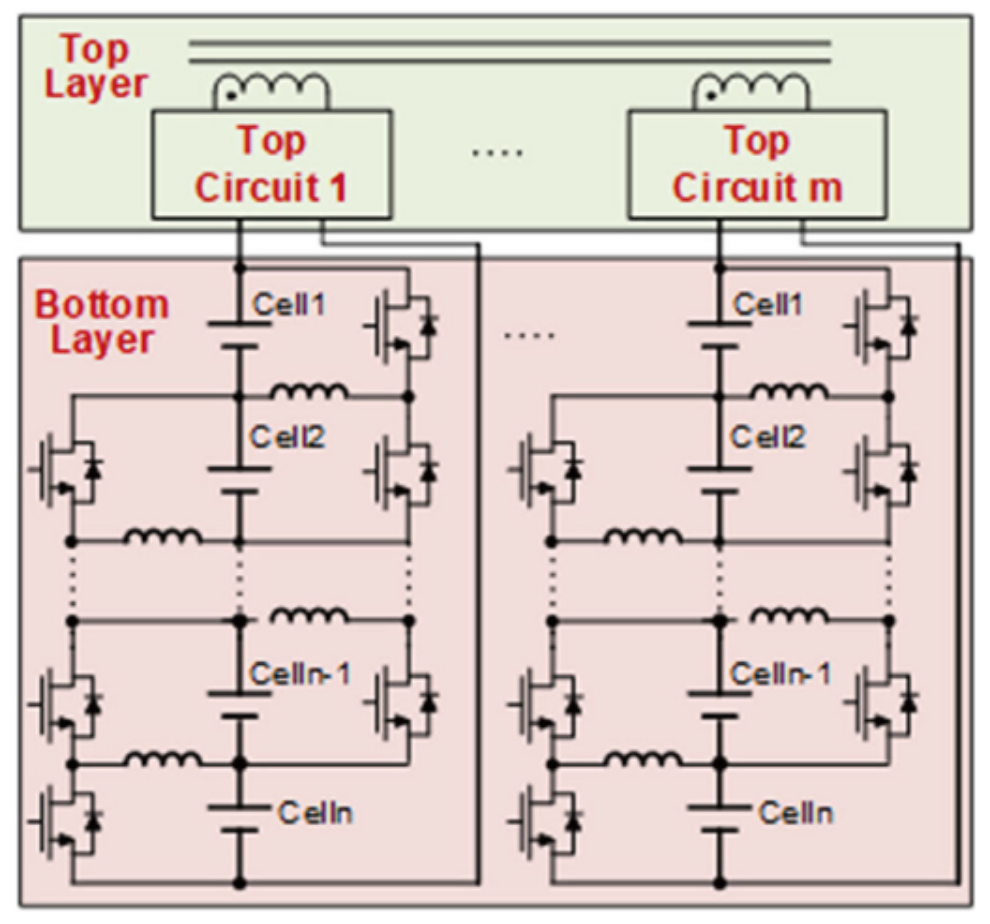
\includegraphics[width=0.6\textwidth]{hbbc_top.png}
        \caption{Topolog\'ia de balanceo jer\'arquica}
        \label{hier_bal_top}
    \end{center}
\end{figure}

\subsubsubsection{Comparaci\'on de topolog\'ias}

La topolog\'ia es el fundamento principal de los sistemas de ecualizaci\'on de
bater\'ias, la misma determina el costo y el tamaño del sistema completo. Una
topolog\'ia eficiente es esencial para extender el ciclo de vida de un pack de
bater\'ias y mejorar su rendimiento efectivamente. Es crucial seleccionar la
topolog\'ia adecuada seg\'un los requerimientos del sistema. 

Las topolog\'ias pasivas tienen las ventajas de ser circuitos simples, de bajo
costo y convenientes de implementar, por lo tanto, han sido ampliamente
adoptados por los \acrshort{VVEE}s. Sin embargo, esta clase de topolog\'ias
generalmente tienen tiempos de balanceo muy lentos y solo disipan energ\'ia
reduciendo la eficiencia del sistema.

Por el otro lado, la topolog\'ia activa es popular gracias a su buena eficiencia
y bajas p\'erdidas de potencia. Comparado con la ecualizaci\'on pasiva, la
topolog\'ia activa puede efectivamente reducir la inconsistencia entre las
capacidades entre celdas y resistencias internas mejorando el tiempo de vida del
pack de bater\'ias y su energ\'ia disponible.
%\newpage
Dentro de los sistemas de balanceo activo, los \acrshort{CBBC}s tienen el
m\'erito de implementar una estrategia muy simple y de bajo costo, con la
contraparte de que los tiempos de ecualizaci\'on son muy bajos. Los
\acrshort{IBBC}s puede transferir energ\'ia de forma bidireccional y tienen una
velocidad de balanceo moderada, pero tienen problemas de \acrshort{EMI} y una
estrategia de balanceo compleja de implementar. \acrshort{TBBC}s pueden proveer
altas corrientes de ecualizaci\'on, con la contraparte de que su manufactura es
compleja debido a la fabricaci\'on de transformadores con devanados
sim\'etricos. Por \'ultimo los \acrshort{PBBC}s tales como los
convertidores reductores-elevadores y Cuk son atractivos gracias a su alta
corriente de balanceo y su f\'acil integrac\'ion en el circuito, sin embargo,
estos resultan complejos y traen apareados estrategias de control complicadas.

Debido a que el esquema pasivo y activo tienen caracter\'isticas muy distintas
entre si, pueden ser aplicados en distintos escenarios seg\'un la aplicaci\'on
en cuesti\'on, por ejemplo, los esquemas pasivos pueden ser implementados en
\acrshort{VVEE}s de baja potencia o en veh\'iculos h\'ibridos mientras que las
topolog\'ias activas son generalmente implementadas en \acrshort{VVEE}s de alta
potencia.

El Cuadro \ref{comp_bal_table} condensa las ventajas y desventajas de cada
topolog\'ia y la Figura \ref{comp_bal_results} muestra un resultado de las
comparanciones entre ellas. 

\begin{table}[h!]
\begin{center}
\begin{tabular}{@{}llcccccc@{}}
\toprule
\multicolumn{2}{l}{Topologias de balanceo}                                                 & Tiempo & Estructura & Control & Eficiencia & Volumen & Costo \\ \midrule
\multirow{4}{*}{\acrshort{CBBC}} & Ecualizacion pasiva                    & 2      & 5                       & 5                     & 1          & 5       & 5     \\
                                                  & Capacitor alternativo                  & 2      & 4                       & 4                     & 4          & 4       & 4     \\
                                                  & Dos capas de capacitores               & 3      & 3                       & 3                     & 3          & 3       & 4     \\
                                                  & Multi-capas de capacitores             & 3      & 2                       & 2                     & 2          & 3       & 3     \\
\acrshort{IBBC}                  & Multiples inductores                   & 4      & 3                       & 3                     & 3          & 2       & 2     \\
\acrshort{TBBC}                  & Multiples devanados & 4      & 2                       & 3                     & 3          & 2       & 2     \\
\multirow{2}{*}{\acrshort{PBBC}} & Cuk                                    & 4      & 2                       & 2                     & 2          & 3       & 2     \\
                                                  & reductor-elevador                      & 4      & 2                       & 2                     & 2          & 3       & 2     \\ \cmidrule(l){2-8}
\end{tabular}
\caption{La clasificaci\'on est\'a puntuada del 1 al 5. Donde 1 es el peor
y 5 el mejor.}
\label{comp_bal_table}
\end{center}
\end{table}

\begin{figure}[h!]
    \begin{center}
        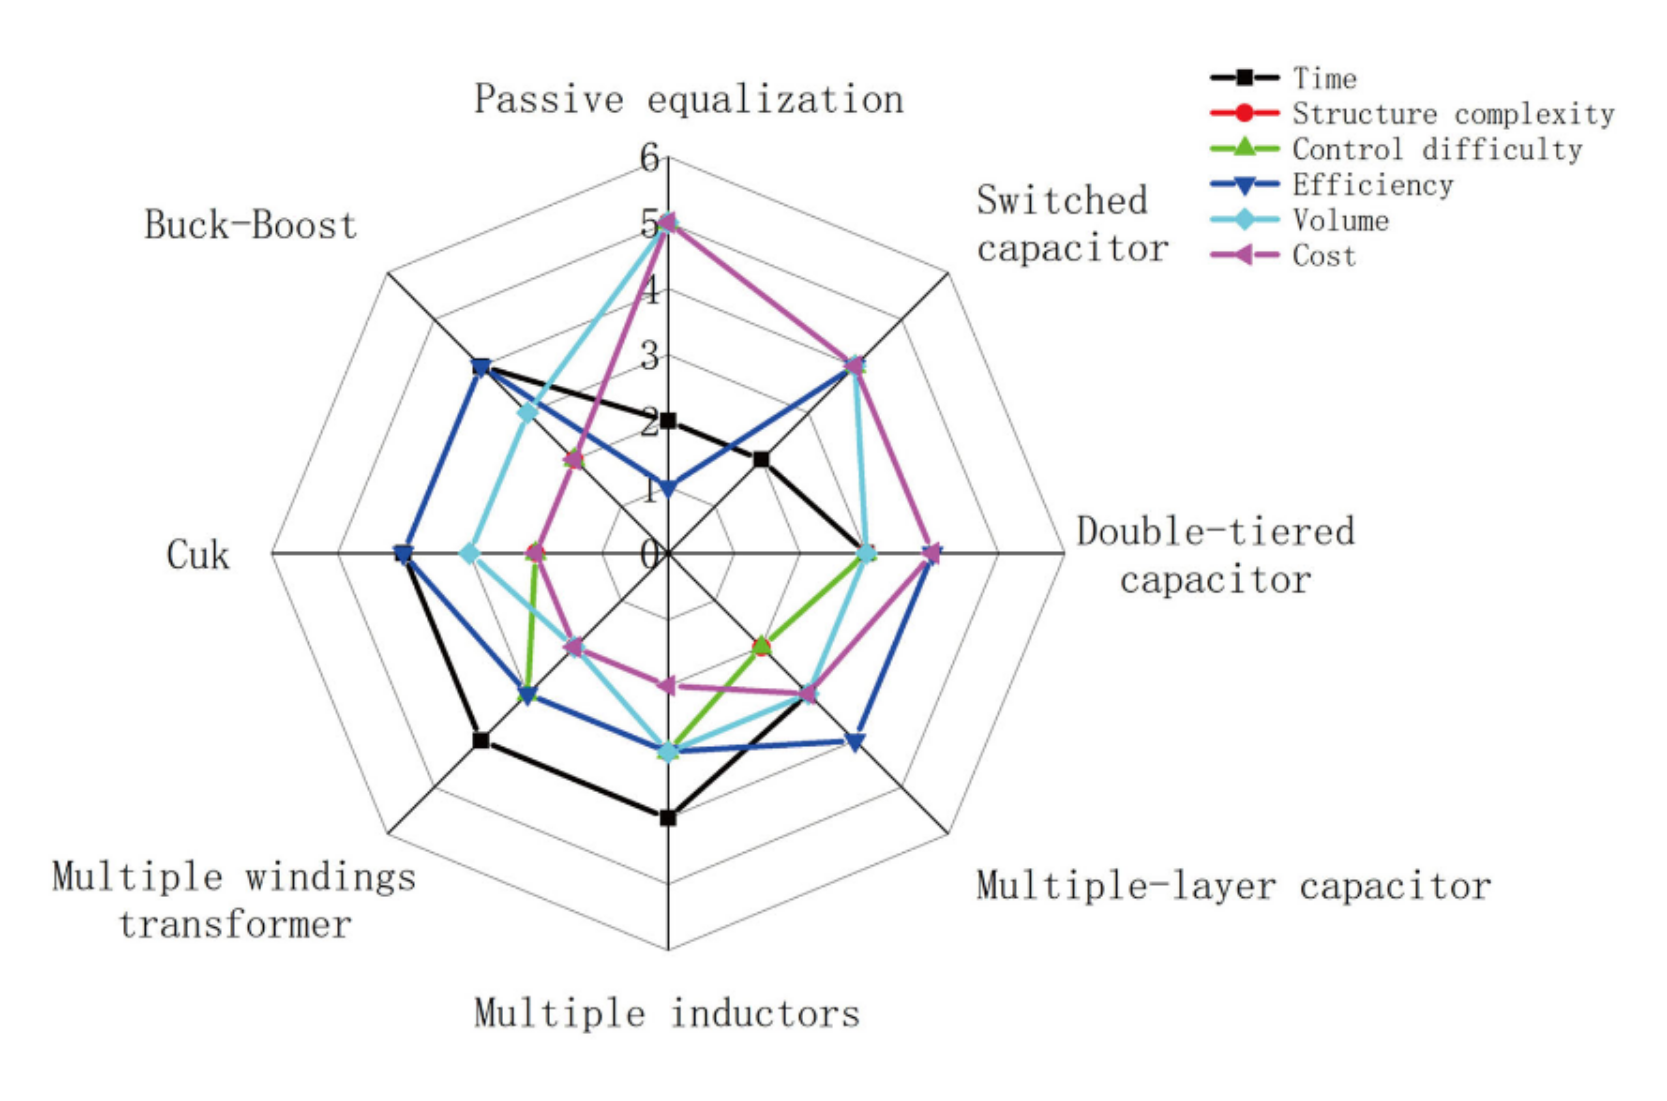
\includegraphics[width=0.8\textwidth]{comp_eq_chart.png}
        \caption{Gr\'afica comparativan de las distintas topolog\'ias disponibles}
        \label{comp_bal_results}
    \end{center}
\end{figure}
%\newpage
\subsubsection{Estrategias de ecualizaci\'on}

Las estrategias de ecualizaci\'on son utilizadas para controlar la operaci\'on
del balanceo teniendo un alto impacto sobre este proceso. Una estrategia de 
ecualizaci\'on inapropiadas para la ecualizaci\'on pueden llevar a problemas de 
desbalanceo o sobrebalanceo, resultando en p\'erdida de potencia innecesaria y 
decaimiento del pack de bater\'ias. Las variables a ecualizar y los algoritmos 
de control son los temas a tener en cuenta en las estrategias de ecualizaci\'on, 
y el desglose de las mismas se puede observar en la Figura 
\ref{eq_strategy_class}.

\begin{figure}[h!]
    \begin{center}
        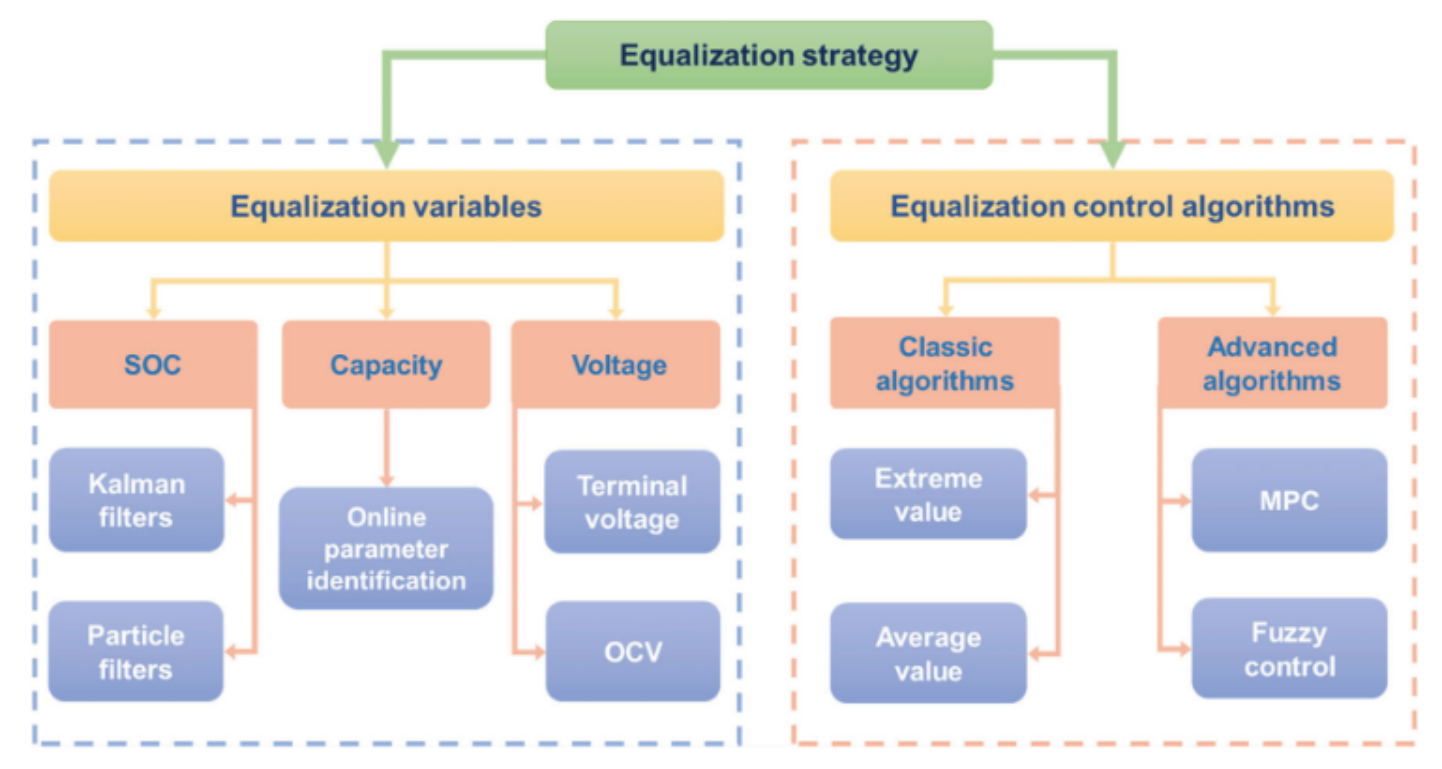
\includegraphics[width=.8\textwidth]{eq_strategy_class.png}
        \caption{Los perfiles de las estrateg\'as de ecualizaci\'on y sus
                 clasificaciones}
        \label{eq_strategy_class}
    \end{center}
\end{figure}

\subsubsubsection{Variables de Ecualizaci\'on}

Las variables de ecualizaci\'on son la base para las estrategias de
ecualizaci\'on. El error de la muestra, el costo computacional y el car\'acter de
hist\'eresis deben ser consideradas a la hora de elegir qué variable ecualizar.
Para la ecualizaci\'on se encuentran tres variables disponibles, el voltaje de 
las celdas, \acrshort{SOC}, capacidad y resistencia interna.

\subsubsubsection{Estrategias de Ecualizaci\'on basadas en voltaje
(\acrshort{VBES})}

Los \acrshort{VBES} (del ingl\'es, \acrlong{VBES}) usan el voltaje de las celdas
medidos en sus terminales por el \acrshort{BMS} como la base para seleccionar
qué bater\'ias deben ser ecualizada. La medición del voltaje en bornes de las
celdas conectadas en serie puede ser realizado de forma directa con una
exactitud aceptable, por lo tanto, los \acrshort{VBES}s son uno de los m\'etodos
viables m\'as b\'asicos a implementar. Sin embargo, las características no
lineales de las celdas de litio, cuestión que se desprende de la Sección
\ref{litioModel} y las particularidades que se presentan a la hora de modelar
una celda, nos permite inferir que el voltaje en bornes no refleja el valor real
\acrshort{OCV} causando dificultades a la hora de utilizar esta variable para
decidir sobre el proceso de ecualizaci\'on de las celdas.

Para subsanar este problema, se propone una estrategia de ecualizaci\'on basada
en el \acrshort{OCV}. Sin embargo, la medici\'on en tiempo real de esta variable
no es viable ya que se necesita un largo tiempo de descanso para que la celda
refleje esta variable en los terminales de la misma.

Debido a que la resistencia interna puede causar una ca\'ida de voltaje
inmediata cuando circula corriente sobre la celda, la diferencia de tensi\'on se
ve afectada a trav\'es de todas las celdas conectadas en serie ante un m\'inimo
est\'imulo sobre ellas. Por lo tanto, esta metodolog\'ia no funcionar\'a
adecuadamente salvo que el veh\'iculo est\'e completamente parado.
Generalmente, este tipo de estrategias son usadas con ternas de celdas de
litio-ion con una linealidad relativa en la curva \acrshort{OCV}-\acrshort{SOC},
pero no son efectivas y corren el riesgo de un desbalanceo cuando son utilizadas
en celdas tipo LiFeP$\mathrm{O_4}$. 

\subsubsubsection{Estrategias de Ecualizaci\'on basadas en la capacidad
(\acrshort{CBES})}

Las \acrshort{CBES} (del ing\'es, \emph{\acrlong{CBES}}) se basan en balancear
la capacidad actual de la bater\'ia. Sin embargo, la capacidad de las bater\'ias
se ven influenciadas por condiciones tales como la corriente y la temperatura
por lo que identificar su valor es complicado y lograr una uniformidad entre
celdas de un pack.

\subsubsubsection{Estrateg\'ia de Ecualizaci\'on basada en el \acrshort{SOC}}

Como se menciona en la secci\'on \ref{algSoc}, el \acrshort{SOC} es una variable
que permite caracterizar la capacidad remanente en una celda. La literatura
actual demuestra que la ecualizaci\'on basada en \acrshort{SOC} puede ser m\'as 
robusta que la basada en voltaje bajo condiciones din\'amicas de operaci\'on.
Sin embargo, el \acrshort{SOC} no puede ser medido de forma directa, si no que
tiene que ser estimado con cierta gravedad de error.

\subsubsubsection{Estrategia de Ecualizaci\'on basada en m\'etodos h\'ibridos}

Este tipo de m\'etodo consiste en tomar ventaja de varias estrategias de
ecualizaci\'on. Por ejemplo, en \cite{ZHANG20194702} se propone el desarrollo de 
un algoritmo h\'ibrido basado en el \acrshort{SOC} y el voltaje, y adopta 
estrategias correspondientes seg\'un distintos rangos de voltaje. Las 
simulaciones muestran resultados de balanceo m\'as eficientes que las basadas 
solamente en el \acrshort{SOC}. 

Por el otro lado, considerando la relaci\'on entre la inconsistencia con la
degradaci\'on de la bater\'ia, el \acrshort{SOC} y el \acrshort{SOH} pueden ser
combinados para obtener un mejor rendimiento de balanceo. Los autores en
\cite{REN2019908} presentan un sistema de ecualizaci\'on h\'ibrido que consiste 
en acoplar la estimaci\'on de ambas variables. Los resultados de las 
simulaciones realizadas demuestran que un m\'etodo de balanceo activo puede 
mejorar el desbalance del \acrshort{SOC} entre celdas.

\subsubsubsection{Comparaci\'on de las variables de control}

Como se menciona anteriormente, la variable a controlar para realizar la
ecualizaci\'on del pack de bater\'ias es crucial para lograr un balanceo
eficiente. La ecualizaci\'on basada en el voltaje de cada celda es el m\'etodo
m\'as f\'acil de implemetar ya que su medicion se puede realizar de forma
directa, sin embargo, lleva apareado una gran cantidad de inconvenientes, como
por ejemplo, la polarizaci\'on de la celda y el error de la medici\'on pueden
llevar a que el balanceo sea ineficiente poniendo en riesgo la salud del pack
de bater\'ias. Por el otro lado, las estrategias basadas en \acrshort{SOC} y
capacidad de la bater\'ia tienen el beneficio de poder determinar un desbalanceo
de forma m\'as eficiente pero bajo el costo de necesitar un sistema de
c\'omputos que permita estimar las variables bajo estudio. Finalmente, surgen
los m\'etodos h\'ibridos que se encargan de fusionar ambas variables, como el
voltaje y el \acrshort{SOC} para combinar ambas ventajas y obtener una
ecualizaci\'on m\'as robusta del sistema.

\subsubsection{Algoritmos de control para la ecualizaci\'on}

Los algoritmos de control son cruciales para el rendimiento de la
ecualizaci\'on, son utilizados para determinar el tiempo de balanceo y
corriente. Generalmente, estos algoritmos se pueden dividir en dos grupos:
algoritmos cl\'asicos de control (\acrshort{CCA}, del ingl\'es \acrlong{CCA}) y
algortimos avanzados de control (\acrshort{ACA}, del ingl\'es \acrlong{ACA}).
Estos algoritmos son posibles de implementar en determinados casos y deben ser
seleccionados acorde al costo computacional, intervalo de muestreo y el nivel de
robustez requerido.

\subsubsubsection{Algortimos cl\'asicos de control}

Los \acrshort{CCA}s realizan operaciones matem\'aticas basadas en las variables
de ecualizaci\'on selccionadas. Normalmente, los \acrshort{CCA}s utilizan el
resultado de operaciones aritm\'eticas cl\'asicas tales como el promedio,
desviaciones estandards y varianzas como los criterios de ecualizaci\'on. Debido
a las ventajas en flexibilidad de c\'alculo y f\'acil implementaci\'on estos
m\'etodos han sido adoptados en aplicaciones de \acrshort{VVEE}s en las
\'ultimas d\'ecadas.

El algoritmo de ecualizaci\'on basado en valores extremos (\acrshort{EVEA}, del
ingl\'es \emph{\acrlong{EVEA}}) aplica los extremos de la variable de ecualizaci\'on
como el objetivo de balanceo. Los \acrshort{EVEA}s son b\'asicos y efectivos con 
un costo computacional bastante limitado, sin embargo suelen tener problemas de
desbalanceo debido a que no son robustos en casos como en la que la diferencia
entre ambos extremos no es lo suficiente grande, el sistema puede llegar a
sobre-balancear el sistema y degradar el rendimiento de la bater\'ia.

El algoritmo de ecualizaci\'on basado en el valor promedio (\acrshort{AVAE}, del
ingl\'es \emph{\acrlong{AVAE}}) calcula el promedio de la variable de
ecualizaci\'on seleccionada y despu\'es utiliza el criterio del valor promedio
para implementar la l\'ogica de balanceo. Este tipo de algoritmo es usado
ampliamente en \acrshort{VVEE}s debido a que son simples y confiables. La
eficiencia de ecualizaci\'on y el tiempo de balanceo puede verse afectado por
las variables seleccionadas, que deben ser consideradas cuidadosamente basado en
condiciones espec\'ificas.

\subsubsubsection{Algoritmos de control avanzado}

Muchos de los m\'etodos avanzados de control, como por ejemplo el control
predictivo y el control por l\'ogica difusa fueron implementados en muchas
aplicaciones de ecualizaci\'on.

El control predictivo es un m\'etodo de la teor\'ia de control avanzada que usa
una optimizaci\'on m\'ovil en tiempo real para predecir los cambios din\'amicos
y ajustar el control acorde a estos cambios, logrando en todo punto de 
operaci\'on un \'optimo rendimiento en el balanceo. Comparado con los
algoritmos de optimizaci\'on, el control predictivo tiene menor costo
computacional y ha sido usado ampliamente en sistemas de control no lineales.
Este m\'etodo puede subsanar la no linealidad de las celdas de litio, ya que
pueden predecir el estado de la bater\'ia y el offset de polarizaci\'on.
Comparado con un control promedio de \acrshort{SOC}, el mismo puede converger a
\acrshort{SOC}s y voltajes m\'as uniformes evitando de esta forma cualquier tipo
de sobre-balanceo.

El control basado en l\'ogica difusa es otro control perteneciente a la teor\'ia
del control avanzado que procesa informaci\'on imprecisa que depende de un grado
de conocimiento del sistema. En \cite{jia_et_al_fuzzy} se propone un controlador 
de tipo fuzzy que utiliza como entrada el nivel de desbalanceo y la corriente de 
carga que circula por el pack de bater\'ias. Los resultados demuestran que este 
m\'etodo es robusto y puede ecualizar el sistema en un tiempo corto.

Por \'ultimo, en la literatura se propuso el uso de redes neuronales,
controladores tipo PID y algoritmos acoplados como potenciales algoritmos de
control para mejorar el rendimiento del balanceo.

\subsubsubsection{Comparaci\'on de algoritmos de control}

Los algoritmos basados en el control cl\'asico fueron las primeras
implementaciones de balanceo utilizadas en \acrshort{VVEE}s debido a sus 
ventajas en cuanto a la baja complejicidad de implementaci\'on. Sin embargo, 
\'estos son propensos a causar desbalanceos debido a factores relacionados al 
ruido y al error de muestreo asociado con el l\'imite computacional para 
sistemas embebidos en \acrshort{VVEE}s.

Adicionalmente, los algoritmos de control avanzado tambi\'en son ampliamente
utilizados en aplicaciones de almacenamiento de energ\'ia en celdas de
litio-ion. Son caracterizados por tener una r\'apida convergencia, estabilidad y
robustos, mejorando los problemas de sobre y desbalanceo de celdas. Sin embargo,
estos sistemas est\'an apareados a un alto costo computacional, y el rendimiento
del control depende exclusivamente de la precisi\'on del modelo, que es
complicado de obtener.

\subsection{Sensado de Corriente}

El sensado de la corriente de carga como de descarga del pack de batería juega
un rol muy importante en el desarrollo exitoso de un \acrshort{BMS}. Es a partir
de conocer con precisión la magnitud de corriente que el sistema podrá mantener
el pack de baterías operando dentro de la zona segura (\acrshort{SOA} por sus
siglas en ingles), monitorear la distribución de carga entre las celdas,
implementar correctamente los algoritmos de ecualización de carga y mantener un
seguimiento preciso del estado de carga.

\noindent Existen en el mercado una gran variedad de tecnologías y 
soluciones para la medición de corriente en las diferentes aplicaciones. 
Algunas de las tecnologías más relevantes, disponibles en el mercado son:
\begin{itemize}
    \item Resistencia Shunt
    \item Transformadores de intensidad (TI)
    \item Bobina de Rogowski 
    \item Sensores de Efecto Hall
    \item Sensores de Impedancia Magnética (MI)
    \item Sensores de Magnetoresistencia Gigante 
    \item Sensores Ópticos (Experimental)
\end{itemize}

Dentro del amplio abanico de métodos y tecnologías utilizadas para la medición
de corrientes los dos más elegidos e implementados en Sistemas de Administración
de Baterías \acrshort{BMS} son las mediciones a partir de resistencias Shunt y
mediciones a partir de sensores de efecto hall debido a las caracter\'isticas de
ambas metodolog\'ias.

\subsubsection{Resistencia Shunt}

La tecnología Shunt se vale del Sensado de la caída del voltaje sobre una
resistencia de unos pocos mili ohmios en serie con el paso de la corriente
incógnita para la medición indirecta de la corriente.

El método de sensado por resistencia tipo shunt presenta una de las mejores
relaciones costos-efectividad, presentando un empaquetado compacto y aplicable
en mediciones de corrientes tanto continua como alterna encontrando su
frecuencia de corte por encima de las decenas de Mhz.

Las mediciones por resistencia shunt carecen naturalmente de aislación galvánica
debiendo ser resuelta a partir del circuito de implementación. Generalmente, los
shunts presentan bajo coeficiente de temperatura de resistencia, (\acrfull{TCR}
por sus siglas en ingles). Característica fundamental en las implementaciones de
\acrshort{BMS} en sistemas de vehículos eléctricos que permite aumentar el rango
de temperatura de operación del sistema.

Aunque los shunts de corrientes operen bajo el principio de caida de voltaje
ohmico, en la práctica las resistencias presentan una inductancia intrínseca que
comprometen la precisión y el ancho de banda máximo de las mediciones.

\subsubsection{Sensor de efecto Hall}

El sensor de efecto Hall es un sensor de efecto magnético basado en el fenómeno
físico homónimo que le da su nombre.  El sensor de efecto Hall es un dispositivo
aislado, no intrusivo que puede ser utilizado para medir corriente tanto
continua como alterna de hasta unos cientos de kHz. El sensor Hall puede ser
fabricado utilizando tecnología CMOS convencional pero a un costo mayor que las
implementaciones con transformadores de corriente o bobinas de Rogowski.

El traductor de efecto Hall encuentra normalmente su límite de medición en los
picos de corriente debido al fenómeno de saturación magnética del núcleo y
encuentra su límite de ancho de banda en las frecuencias menores al MHz. A su
vez, esta tecnología es sumamente sensible a la influencia de los campos
magnéticos externos. Frente a estas limitaciones es común que los sensores de
efecto Hall se implementen mayoritariamente con bobinas cerradas para lograr una
mejor precisión y un rango mayor de operación dinámico.

El voltaje de offset presente en la medición del dispositivo es poco estable y
varia fuertemente frente a las variaciones de temperatura de operación.

\begin{figure}[h!]
    \centering
    \begin{subfigure}[b]{0.4\linewidth}
	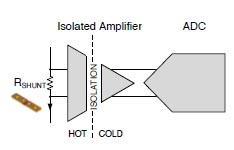
\includegraphics[width=\linewidth]{../assets/R-Shunt_Isolated_Sensor.jpg}
	\caption{Sensado por Resistencia Shunt}
    \end{subfigure}%
    \hspace{15mm}
    \begin{subfigure}[b]{0.4\linewidth}
	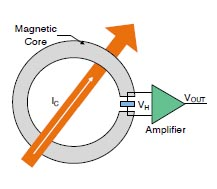
\includegraphics[width=\linewidth]{../assets/Open-loop_Hall_Sensor.jpg}
	\caption{Sensado por efecto Hall de loop abierto}
    \end{subfigure}
    \caption{Diagramas - Métodos de sensado de corriente}
    \label{fig:SenseMetods}
\end{figure}

\newpage

\subsection{Protocolos de comunicación}
En la actualidad es innegable la expansión de la tecnología y la electrónica haciendose más presentes en nuestro día a día, hoy no es raro escuchar de domótica, IoT y Smart Devices.Los vehículos no son la excepción y aún en los vehículos de 4 plazas de gamma baja se integran un conjunto de sensores, actuadores y controladores electrónicos.
Estos dispositivos se hayan interconectados entre sí por redes de comunicación transmitiendo señales en tiempo real y recabando información y controlando los diversos procesos que ocurren permanentemente en el vehiculo. Así como también reportando fallas al usuario permitiendo tomar deciciones anticipadas, facilitando el mantenimiento de la unidad.

En los vehiculos actuales los protocolos más utilizados en los vehículos son \acrshort{CAN}, por sus siglas en inglés \acrfull{CAN},  (tanto de alta como de baja velocidad), \acrshort{LIN} del inglés, \acrfull{LIN} y \acrshort{MOST} del inglés, \acrfull{MOST} \cite{Vela2016}.

Dentro del vehículo hallamos sistemas de naturaleza muy variada, por ejemplo, el sistema de frenos ABS, el cierre centralizado, las luces de interior y el canal de audio del sistema de sonido. Cada uno de los cuales tiene requerimientos totalmente distintos, en el caso del sistema ABS los tiempos de reacción deben ser del orden del milisegundo pero con un volumen de datos mínimo, mientras que por el contrario el sistema de sonido tiene un volumen de datos mucho mayor con una prioridad mucho menor ya que es un sistema de entretenimiento y no de seguridad.

De los protocolos mencionados el más utilizado por su superadora relación costo-confiabilidad es el protocolo \acrshort{CAN}, debido a la arquitectura multiplexada con un único bus serie que reduce costos combinada con algoritmos de detección de errores que brindan confiabilidad a la red. Otra de las ventajas de CAN es que si un dispositivo sale de servicio la red continua funcionando perfectamente, además de contar con control de acceso al medio con prioridad. Todo esto hace de CAN un protocolo que desde sus orígenes es óptimo para el rubro automotríz.

\subsubsection{Protocolo CAN}
Este es un protocolo desarrollado inicialmente por la empresa alemana Robert Bosch GmbH en 1983 la cual fue aceptada ampliamente y que posterior mente fue definida como estándar que en su especificación ISO 11898 describe como la información será transmitida entre los diferentes dispositivos de red.

Las principales características de este protocolo son \cite{RBG1991}:
\begin{itemize}
	\item Priorización de mensajes
	\item Sistema Multi-Maestro
	\item Configuración Flexible
	\item Velocidad de transmisión media (hasta 1 Mbit/s)
	\item Señalización y detección de fallas.
\end{itemize}

Para  detectar  errores  a  nivel  de  mensajes  el  protocolo  implementa  tres  
mecanismos: chequeo de redundancia cíclica (CRC), chequeo de formato de trama y 
acuse de recibo (ACK).

Para detectar errores a nivel de bit el protocolo implementa dos mecanismos: 

\begin{itemize}
	\item Monitoreo. Cada nodo transmisor monitorea el nivel del bus a fin 
de detectar la diferencia entre el bit enviado y el recibido. 
	\item Bits de Relleno (Bit stuffing). CAN utiliza la codificación NRZ (no 
retorno a cero) y la técnica de bit  stuffing,  que consiste en insertar un bit complementario cada cinco bits iguales consecutivos transmitidos. 
\end{itemize}

Trabaja en según el modelo \acrshort{OSI} (\acrfull{OSI}) en la primera y la segunda capa, también conocidas como la capa física y la capa de enlace de datos respectivamente.

El protocolo CAN  sólo define las dos primeras capas del Modelo \acrshort{OSI} (\acrfull{OSI}) (física y enlace), aunque no especifica la interfaz al medio físico (Medio de transmisión, conectores).La norma ISO 11898 es el estándar internacional para la comunicación de alta velocidad usando el protocolo de bus CAN. Esencialmente este estándar define las capas física y de enlace de datos.

\subsubsubsection{Capa Física} 
La capa física en \acrshort{CAN} es responsable de la transferencia de bits entre los distintos nodos que componen la red. Define aspectos como, niveles de señal, codificación, sincronización y tiempos en que los bits se transfieren al bus.
En la especificación original de \acrshort{CAN}, la capa física no fue definida, permitiendo diferentes opciones para la elección del medio y niveles eléctrico de transmisión. Las características de las señales eléctricas en el bus fueron establecidas más tarde por el estandar ISO 11898.

La especificación \acrfull{CiA}, complementó las definiciones respecto al medio físico y conectores. Los nodos conectados al bus interpretan dos niveles lógicos denominados:

\begin{itemize}
	
	\item Dominante: La tensión diferencial (CAN-H - CAN-L) es del orden de 2.0V con CAN-H = 3.5V y CAN-L = 1.5V (nominales).\\
	\item Recesivo: La tensión diferencial (CAN-H - CAN-L) es del orden de 0V con CAN-H = 2.5V y CAN-L = 2.5V (nominales).\\
	
\end{itemize}

La topología es bus con derivaciones de corta longitud.Si se presenta el caso de perdida de prestaciones en cuanto a velocidad o longitud máxima se pueden adoptar topologias en estrella. El bus se cierra en los extremos con impedancias de carga.

El número máximo de nodos no está limitado por la especificación básica y depende de las características de los transreceptores, las especificaciones de buses de campo lo limitan a 32 o 64 en una red sin repetidores.


\subsubsubsection{Capa de Datos}
Unas de las características que distingue a CAN con respecto a otras normas, es su técnica de acceso al medio denominada como 
CSMA/CD+CR o ``Carrier Sense, Multiple Access/Colission Detection + Collision Resolution" (Acceso múltiple con detección de 
portadora, detección de colisión más resolución de colisión). 

El  acceso  al  medio  por  medio  de  técnicas de acceso múltiple y detección de colisión evolucionaron desde el método ALOHA 
inicial  hasta  su  consagración  como  método  de  acceso  al  medio  de  las  redes  Ethernet,  con  técnica  CSMA/CD.    El  método  de  
acceso  al  medio  utilizado  en  bus  CAN  añade  una  característica  adicional:  la  resolución  de  colisión.    En  la  técnica  CSMA/CD  
utilizada en redes Ethernet ante colisión de varias tramas, todas se pierden, CAN resuelve la colisión con la supervivencia de una 
de  las  tramas  que  chocan  en  el  bus.    Además  la  trama  superviviente  es  aquella  a  la  que  se  ha  identificado  como  de  mayor  
prioridad. 

La resolución de colisión se basa en una topología eléctrica que aplica una función lógica determinista a cada bit, que se resuelve 
con la prioridad del nivel definido como bit de tipo dominante.  Definiendo el bit dominante como equivalente al valor lógico '0' y 
bit   recesivo  al   nivel  lógico  '1'  se  trata  de  una  función  AND  de  todos  los  bits  transmitidos  simultáneamente.    Cada  transmisor  
escucha  continuamente  el  valor  presente  en  el  bus,  y  se  retira  cuando  ese  valor  no  coincide  con  el  que  dicho  transmisor  ha  
forzado.    Mientras  hay  coincidencia  la  transmisión  continua,  finalmente  el  mensaje  con  identificador  de  máxima  prioridad  
sobrevive.  Los demás nodos reintentarán la transmisión lo antes posible.\\

\subsubsubsection{Mensajes y Tipos de Tramas}
CAN utiliza mensajes de estructura predefinida, tramas, para la gestión de la comunicación.
Se distinguen entre dos variantes de CAN, el definido en CAN 2.A o ``CAN Standard" y el definido en CAN 2.B o ``CAN
Extendido", los formatos de trama son análogos diferenciándose básicamente en el número de bits que se utiliza para el
identificador de mensaje: 11 bits (2032 identificadores) diferentes en CAN Standard y 29 bits (536.870.912 identificadores) en
CAN Extendido.
Las tramas CAN son de longitud reducida, la trama más larga es de 130 bits en CAN Estándar y 154 bits en CAN Extendido.
Los tipos de trama, y estados de bus, utilizados segun \cite{KaschelHector2004} son:
\begin{itemize}
	\item Trama de datos: la que un nodo utiliza normalmente para poner información en el bus (siempre es un ``broadcast" a todos los demás nodos). Puede incluir entre 0 y 8 Bytes de información útil.\\
	\item Trama de interrogación remota (en lo que sigue se denominará como trama remota (``remote frame"): puede ser utilizada por
	un nodo para solicitar la transmisión de una trama de datos con la información asociada a un identificador dado. El nodo que
	disponga de la información definida por el identificador la transmitirá en una trama de datos.\\
	\item Tramas de error: usadas para señalar al resto de nodos la detección de un error, invalidando el mensaje erróneo normalmente (un caso especial es un nodo en estado de ``error pasivo").\\
	\item Trama de sobrecarga: permite que un nodo fuerce a los demás a alargar el tiempo entre transmisión de tramas sucesivas
	Espaciado inter-tramas: Las tramas de datos (y de interrogación remota) se separan entre sí por una secuencia predefinida que
	se denomina espaciado inter-trama.\\
	\item Bus en reposo: En los intervalos de inactividad se mantiene constantemente el nivel recesivo del bus.\\
	\end{itemize}


\begin{comment}

En un bus CAN los nodos transmiten la información espontáneamente con tramas de datos, bien sea por un proceso cíclico o activado ante eventos en el nodo. La trama de interrogación remota sólo se suele utilizar para detección de presencia de nodos o para puesta al día de información en un nodo recién incorporado a la red. Los mensajes pueden entrar en colisión en el bus, el de identificador de mayor prioridad sobrevivirá y los demás son retransmitidos lo antes posible.



\subsubsubsection{Formatos de Trama}

	\textbf{Trama de Datos}\\
	Una trama de datos es generada por un nodo CAN cuando transmite información. Los campos incluidos en una trama de datos
	son para CAN Estándar.
	
	\begin{itemize}
	\item \textbf{Inicio de trama (SOF):} El inicio de trama es un campo de un solo bit siempre dominante que indica el inicio de la transmisión. Los nodos receptores se sincronizan con el flanco de bajada de este bit.\\
	\item \textbf{Arbitraje:} El campo de identificación está formado por el identificador de mensaje (11 bits) más el bit RTR. En una trama de datos el bit RTR es dominante. En una trama remota es recesivo. Los bits de identificador se transmiten en orden de más significativo a menos significativo.\\
	\item \textbf{Control:} El campo de control está formado por dos bits reservados para uso futuro y cuatro bits adicionales que indican el número de bytes de datos. En realidad el primero de estos bits (IDE) se utiliza para indicar si la trama es de CAN Estándar (IDE dominante) o Extendido (IDE recesivo). El segundo bit (RB0) es siempre recesivo. Los cuatro bits de código de longitud (DLC) indican en binario el número de bytes de datos en el mensaje (0 a 8).\\
	\item \textbf{Datos:} Es un campo formado por 0 a 8 bytes de datos, es decir 0 a 64 bits en saltos de 8. Cada byte se transmite con bit más significativo primero.\\
	\item \textbf{CRC:} Código de redundancia cíclica que genera el transmisor por la división módulo 2 de todos los bits precedentes del mensaje, incluyendo los de relleno si existen, por el polinomio generador: X15+ X14+ X8+ X7+ X4+ X3+ X1+1, el resto de esta división es el código CRC transmitido. Los receptores comprueban este código. Tras el código CRC se incluye un bit recesivo (delimitador de CRC).\\
	\item \textbf{Campo de reconocimiento (ACK):} es un campo de dos bits que el transmisor pone como recesivos. El primero de estos bits se
	sobreescribe por un bit dominante de reconocimiento transmitido por los nodos que han recibido el mensaje correctamente. El bit
	de ACK queda así insertado entre dos bits dominantes de delimitación.
	\item \textbf{Fin de trama (EOF)}: Cierra la trama, consiste en 7 bits recesivos sucesivos.\\
	\item \textbf{Espaciado entre tramas (IFS)}. Consta de un mínimo de 3 bits recesivos.\\
\end{itemize}

La trama de datos de CAN Extendido se diferencia de la de CAN Estándar en que un bit dominante fijo (SRR) aparece en la posición del bit RTR de CAN Estándar, se fija el bit IDE como recesivo, siguen luego los 18 bits adicionales del identificador, el campo de control con RTR, dos bits reservados y la longitud de datos y el resto de la trama es análogo.\\

En un bus CAN pueden convivir nodos CAN Estándar y CAN Extendido, para ello los nodos CAN Estándar han de ser del tipo CAN 2.OB Pasivo, estos nodos reaccionan ignorando tramas CAN Extendido en lugar de señalarlas como erróneas. Los nodos que cumplen CAN 2.0B pueden funcionar en modo Estándar o Extendido indistintamente.
Durante este trabajo se hará referencia sobre todo a CAN Estándar, en todo caso las diferencias con CAN Extendido son mínimas,
excepto la posibilidad de contar con un número mucho mayor de identificadores disponibles.\\

\textbf{Trama remota}\\

El formato es análogo a la trama de datos pero con el bit RTR recesivo . Por otra parte una trama remota no incluye nunca datos.
El identificador es el del mensaje que se solicita, el campo longitud corresponde a la longitud de ese mensaje.\\

\textbf{Trama de error}\\

Las tramas de error son generadas por cualquier nodo que detecta un error. Consiste en dos campos: Indicador de error (``Error
Flag") y Delimitador de error. El delimitador de error consta de 8 bits recesivos consecutivos y permite a los nodos reiniciar la
comunicación limpiamente tras el error. El Indicador de error es distinto según el estado de error (los estados de error de nodo se
describirán en páginas sucesivas) del nodo que detecta el error:
Si un nodo en estado de error ``Activo" detecta un error en el bus interrumpe la comunicación del mensaje en proceso generando
un "Indicador de error activo" que consiste en una secuencia de 6 bits dominantes sucesivos. Esta secuencia rompe la regla de
relleno de bits y provocará la generación de tramas de error en otros nodos. Por tanto el Indicador de error puede extenderse entre
6 y 12 bits dominantes sucesivos. Finalmente se espera el campo de delimitación de error formado por los 8 bits recesivos.
Entonces la comunicación se reinicia y el nodo que había sido interrumpido reintenta la transmisión del mensaje.
Si un nodo en estado de error ``Pasivo" detecta un error, el nodo transmite un ``Indicador de error pasivo" seguido, de nuevo, por el
campo delimitador de error. El indicador de error de tipo pasivo consiste en 6 bits recesivos seguidos y, por tanto, la trama de
error para un nodo pasivo es una secuencia de 14 bits recesivos. De aquí se deduce que la transmisión de una trama de error de ti
o pasivo no afectará a ningún nodo en la red, excepto cuando el error es detectado por el propio nodo que está transmitiendo. En
ese caso los demás nodos detectarán una violación de las reglas de relleno y transmitirán a su vez tramas de error.
Tras señalar un error por medio de la trama de error apropiada cada nodo transmite bits recesivos hasta que recibe un bit también
recesivo, luego transmite 7 bits recesivos consecutivos antes de finalizar el tratamiento de error.\\

\textbf{Espacio entre tramas}\\

El espacio entre tramas separa una trama (de cualquier tipo) de la siguiente trama de datos o interrogación remota. El espacio
entre tramas ha de constar de, al menos, 3 bits recesivos. Esta secuencia de bits se denomina ``íntermission". Una vez transcurrida
esta secuencia un nodo en estado de error activo puede iniciar una nueva transmisión o el bus permanecerá en reposo. Para un
nodo en estado error pasivo la situación es diferente, deberá espera una secuencia adicional de 8 bits recesivos antes de poder
iniciar una transmisión. De esta forma se asegura una ventaja en inicio de transmisión a los nodos en estado activo frente a los
nodos en estado pasivo.\\

\textbf{Trama de sobrecarga}\\

Una trama de sobrecarga tiene el mismo formato que una trama de error activo. Sin embargo, la trama de sobrecarga sólo puede
generarse durante el espacio entre tramas. De esta forma se diferencia de una trama de error, que sólo puede ser transmitida
durante la transmisión de un mensaje. La trama de sobrecarga consta de dos campos, el Indicador de Sobrecarga, y el delimitador.
El indicador de sobrecarga consta de 6 bits dominantes que pueden ser seguidos por los generados por otros nodos, dando lugar a
un máximo de 12 bits dominantes. El delimitador es de 8 bits recesivos.
Una trama de sobrecarga puede ser generada por cualquier nodo que debido a sus condiciones internas no está en condiciones de
iniciar la recepción de un nuevo mensaje. De esta forma retrasa el inicio de transmisión de un nuevo mensaje. Un nodo puede
generar como máximo 2 tramas de sobrecarga consecutivas para retrasar un mensaje. Otra razón para iniciar la transmisión de
una trama de sobrecarga es la detección por cualquier nodo de un bit dominante en los 3 bits de "intermission". Por todo ello una
trama de sobrecarga de generada por un nodo dará normalmente lugar a la generación de tramas de sobrecarga por los demás
nodos dando lugar, como se ha indicado, a un máximo de 12 bits dominantes de indicador de sobrecarga.\\

\textbf{Arbitraje}\\

Cada nodo que transmite, a su vez está monitoreando el dato que se refleja en el bus y se contrasta con el dato enviado por el mismo, en caso de no coincidir esto quiere decir que el transmisor de mayor prioridad es él mismo y continua la transmisión, de lo contrario detectará que hay un mensaje de mayor prioridad en el bus y lo leerá.

\end{comment}






\section{Desarrollo}\label{desarrollo}

En \'esta secci\'on se explaya el desarrollo matem\'atico y la implementaci\'on 
f\'isica del \acrshort{BMS}, incluyendo el pack de bater\'ias, el modelo 
matem\'atico de la celda de litio-ion junto a sus algortimos de estimaci\'on de 
\acrshort{SOC} y ecualizaci\'on de celdas, mostrando los resultados de las
simulaciones y, finalmente, el desarrollo del hardware y firmware necesario para
implementar los distintos componentes del sistema en un sistema f\'isico real.

\subsection{Espíritu del proyecto}

El desarrollo del proyecto se funda sobre bases de espíritu colarborativas, bajo
la filosofía de codigo abierto y de software libre. Fuera del paragua de alguna
licencia en particular. Tanto los archivos fuentes del proyecto, de software y
hardware, como la extensa y profunda documentación del mismo se encuentran
disponibles para quienes deseen estudiarlos, modificarlos, ejecutarlos y
redistribuirlos citando la fuente debidamente. 

El proyecto no persigue fines comerciales ni onerosos de ningún tipo y pretende
ser una nueva pieza en el reducido ecosistema de los \acrshort{BMS}s de
codigo/hardware abierto.

El hardware y el software desarrollado se orientan a servir como plataforma de
ensayo y desarrollo de futuros proyectos que partan de este \acrshort{BMS}. Con
el objetivo de que la disposición de la documentación funcione como la
herramienta que lo permita.

\subsection{Pack de bater\'ias}\label{battery_pack}

Como se menciona en la secci\'on \ref{proy_specs}, el pack de bater\'ias a
controlar posee 6 m\'odulos conectados en serie, donde cada m\'odulo est\'a
compuesto por 3 celdas de litio-ion conectadas en paralelo. En este caso, el pack
de bater\'ias est\'a conformado por celdas de litio-ion modelo NCR18650PF. La
arquitectura del pack se puede observar en la Figura \ref{pack_bateria} y una
im\'agen de la celda se muestra en la Figura \ref{foto_bateria}

\begin{figure}[h!]
    \begin{subfigure}[b]{.5\textwidth}
	\begin{center}
	    \begin{minipage}[c]{0.45\textwidth}
		\centering
		\begin{circuitikz}[european]

		    \draw (7, 2) -- (7, 2.2);
		    \draw (7, 2) to[battery1] (7, 1.6);
		    \draw (7, 1.4) -- (7, 1.6);
		    \draw (7, 1.4) to[battery1] (7, .9);			
		    \draw (7, .7) -- (7, .9);			
		    \draw (7, 0.7) to[battery1] (7, 0.2);			
		    \draw (7, 0.2) -- (7, -0.2);
		    \draw (7, -0.2) to[battery1] (7, -0.7);
		    \draw (7, -.7) -- (7, -.9);
		    \draw (7, -.9) to[battery1] (7, -1.4);
		    \draw (7, -1.4) -- (7, -1.6);
		    \draw (7, -1.6) to[battery1] (7, -2);
		    \draw (7, -2) -- (7, -2.2);

		    \draw (9, 2) -- (9, 2.2);
		    \draw (9, 2) to[battery1] (9, 1.6);
		    \draw (9, 1.4) -- (9, 1.6);
		    \draw (9, 1.4) to[battery1] (9, .9);			
		    \draw (9, .7) -- (9, .9);			
		    \draw (9, 0.7) to[battery1] (9, 0.2);			
		    \draw (9, 0.2) -- (9, -0.2);
		    \draw (9, -0.2) to[battery1] (9, -0.7);
		    \draw (9, -.7) -- (9, -.9);
		    \draw (9, -.9) to[battery1] (9, -1.4);
		    \draw (9, -1.4) -- (9, -1.6);
		    \draw (9, -1.6) to[battery1] (9, -2);
		    \draw (9, -2) -- (9, -2.2);

		    \draw (11, 2) to[battery1] (11, 1.6);
		    \draw (11, 1.4) -- (11, 1.6);
		    \draw (11, 1.4) to[battery1] (11, .9);			
		    \draw (11, .7) -- (11, .9);			
		    \draw (11, 0.7) to[battery1] (11, 0.2);		
		    \draw (11, 0.2) -- (11, -0.2);
		    \draw (11, -0.2) to[battery1] (11, -0.7);
		    \draw (11, -.7) -- (11, -.9);
		    \draw (11, -.9) to[battery1] (11, -1.4);
		    \draw (11, -1.4) -- (11, -1.6);
		    \draw (11, -1.6) to[battery1] (11, -2);
		    \draw (11, -2) -- (11, -2.2);

		    \draw (7, 0) -- (9, 0);
		    \draw (9, 0) -- (11, 0);

		    \draw (7, 0.8) -- (9, 0.8);
		    \draw (9, 0.8) -- (11, 0.8);

		    \draw (7, 1.5) -- (9, 1.5);
		    \draw (9, 1.5) -- (11, 1.5);

		    \draw (7, 2.2) -- (9, 2.2);
		    \draw (9, 2.2) -- (11, 2.2);			

		    \draw (7, -0.8) -- (9, -0.8);
		    \draw (9, -0.8) -- (11, -0.8);

		    \draw (7, -1.5) -- (9, -1.5);
		    \draw (9, -1.5) -- (11, -1.5);

		    \draw (7, -2.2) -- (9, -2.2);
		    \draw (9, -2.2) -- (11, -2.2);			

		    \draw [dashed] (6.5, 2.4) rectangle (11.5, -2.4);

		    \draw node at (8.2, 2.6) {Pack de Baterías 6s3p};
		\end{circuitikz}
	    \end{minipage}
	\end{center}
	\caption{Esquemático de la arquitectura del pack de baterías.}
	\label{pack_bateria}
    \end{subfigure}%
    \begin{subfigure}[b]{.45\textwidth}
	\centering
	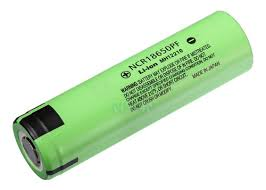
\includegraphics[width=0.7\textwidth]{18650.jpg}
	\caption{Foto celda NCR18650PF.}
	\label{foto_bateria}
    \end{subfigure}
    \caption{Pack 6s3p y Celda NCR18650PF.}
    \label{pack}
\end{figure}
\FloatBarrier

\newpage

\subsubsection{Celda NCR18650PF}

La celda de litio-ion 18650 fue originalmente diseñada para ser utilizada en
bater\'ias de notebooks pero debido a su amplia versatilidad su uso se
expandi\'o hasta ser implementados en \acrshort{VVEE}s. \'Estas bater\'ias se
caracterizan por su tamaño reducido de 18mm de di\'ametro por 65mm de alto,
caracteristicas que le dan su nombre. En el mercado actual, se pueden encontrar
diferentes versiones del mismo modelo debido a que cada uno posee una
composici\'on qu\'imica diferente, dando lugar a las distintas caracter\'isticas
de capacidad y voltaje que se descrien a continuaci\'on:

\begin{itemize}
    \item \textbf{LiFePO4}: Fosfato de hierro y litio o tambi\'en conocidas como
        IFR, LFP o Li-fosfato.
    \item \textbf{LiMn2O4}: Oxido de litio manganesio o tambi\'en conocidas como
        IMR, LMO o Li-manganesio.
    \item \textbf{LiNiMnCoO2}: Litio manganesio n\'iquel o tambi\'en conocidas como
        INR o NMC
    \item \textbf{LiNiCoAl2}: Oxido de Litio n\'iquel cobalto aluminio o
        tambi\'en conocidas como NCA o Li-aluminio.
    \item \textbf{LiNiCoO2}: \'Oxido de litio n\'iquel cobalto o tambi\'en
        conocidas como NCO.
    \item \textbf{LiCoO2}: \'Oxido de litio cobalto o tambi\'en conocido como
        ICR, LCO o Li-cobalto.
\end{itemize}

En este caso, la celda NCR18650PF se caracteriza por su cátodo, cuya composición 
química se basa en el óxido de litio níquel cobalto aluminio 
($\mathrm{LiNiCoAlO_2}$) y, según su hoja de datos \cite{18650pf}, sus 
carateristicas electricas se pueden observar en la Tabla \ref{ncr18650pf_table}.

\begin{table}[h]
    \begin{center}
	\begin{tabular}{|c|l|}
	    \hline
	    \multicolumn{2}{|c|}{Especificaciones el\'ectricas}                          \\ \hline
	    \textbf{Capacidad Específica}                 & 2700mAh                            \\ \hline
	    \multirow{2}{*}{\textbf{Capacidad}}           & Mínimo: 2750mAh                    \\ \cline{2-2} 
	    & Tipico: 2900mAh                    \\ \hline
	    \textbf{Corriente de Descarga Máxima}         & 10000mAh($\sim$3.5C)               \\ \hline
	    \textbf{Rango operativo de tensión}           & 2.5V - 4.2V                        \\ \hline
	    \textbf{Voltaje Nominal}                      & 3.6V                               \\ \hline
	    \textbf{Charga}                               & CC-CV, Std. 1375mA, 4.20V, 4.0 hrs \\ \hline
	    \textbf{Peso}                                 & 48g                              \\ \hline
	    \multirow{3}{*}{\textbf{Temperatura}}         & Carga: 0 a 45C                     \\ \cline{2-2} 
	    & Descarga: -20 a 60C                \\ \cline{2-2} 
	    & Almacenaje: -20 a 50C              \\ \hline
	    \multirow{2}{*}{\textbf{Densidad Energética}} & Volum\'etrica: 577Wh/l               \\ \cline{2-2} 
	    & Gravim\'etrica: 207wh/kg             \\ \hline
	\end{tabular}%
	\caption{Especificaciones el\'ectricas de una celda de litio NCR18650PF}
	\label{ncr18650pf_table}
    \end{center}
\end{table}

Por el otro lado, \cite{18650pf} también nos provee curvas significativas, de su
operaci\'on como por ejemplo, la curva de carga \emph{(Fig. \ref{cc_cv_18650})}, 
la curva de descarga para distintas corrientes 
\emph{(Fig. \ref{descarga_18650})} y la curva del ciclo de vida típico de la 
batería \emph{(Fig. \ref{life_cycle_18650})}.

La elecci\'on de \'este tipo de celda se debe a principalmente a que el pack a
controlar ya utiliza \'este modelo y, por el otro lado, ya existe un set de 
datos abiertos \cite{Kollmeyer2018} de distintos ensayos sobre el
mismo, con el cual se pueden desarrollar e investigar distintos modelos y 
simulaciones. 

\begin{figure}[h!]
    \begin{subfigure}[t]{.5\textwidth}
	%   		\centering
	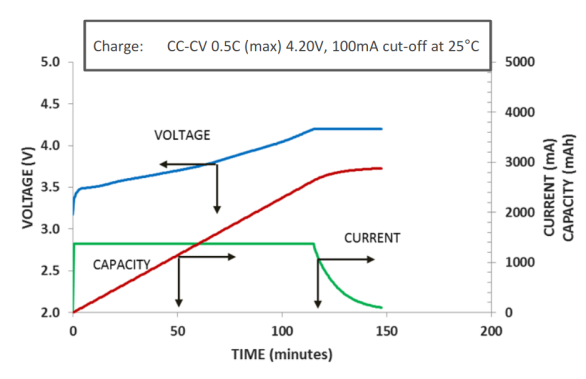
\includegraphics[width=0.9\textwidth]{cc_cv_18650.png}
	\caption{Curva de carga.}
	\label{cc_cv_18650}
    \end{subfigure}%
    ~ 
    \begin{subfigure}[t]{.5\textwidth}
	%    		\centering
	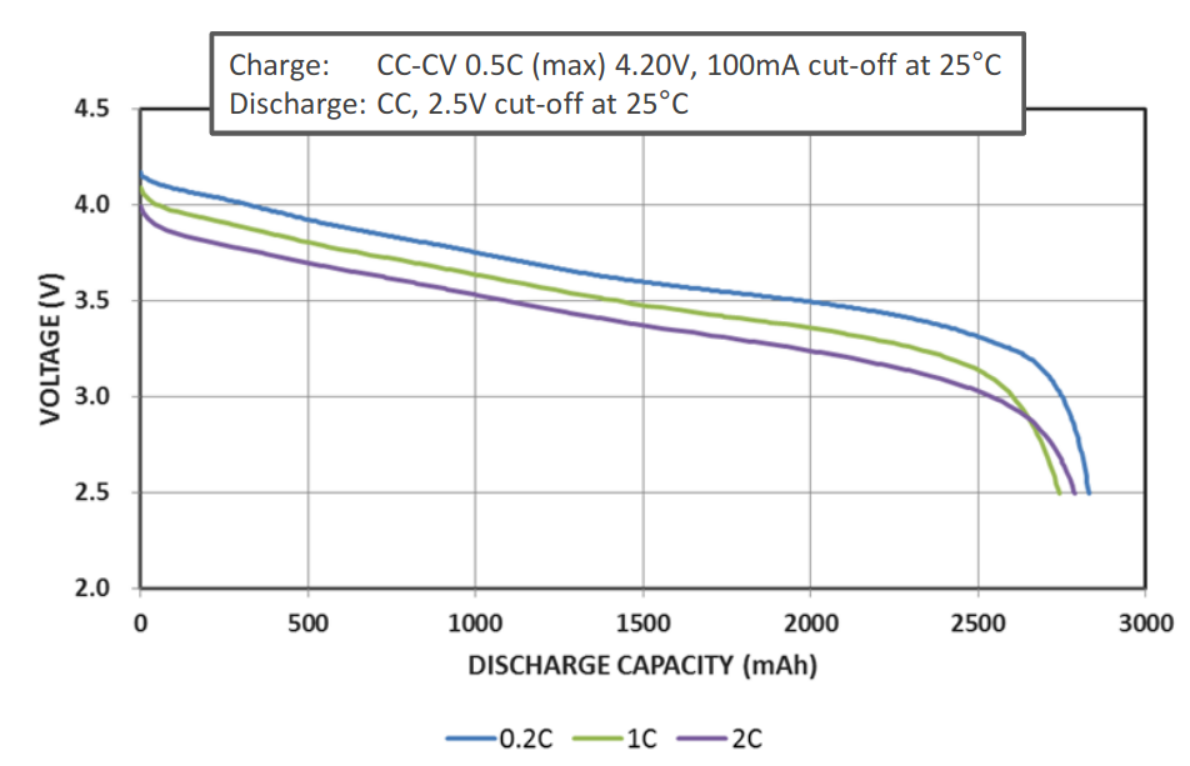
\includegraphics[width=0.9\textwidth]{discharge_18650.png}
	\caption{Curva de descarga en base a distintas corrientes de descarga (0.5C,
	1C, 1.5C y 2C)}
	\label{descarga_18650}
    \end{subfigure}
    ~ 
    \begin{centering}
	\begin{subfigure}[t]{1\textwidth}
	    \centering
	    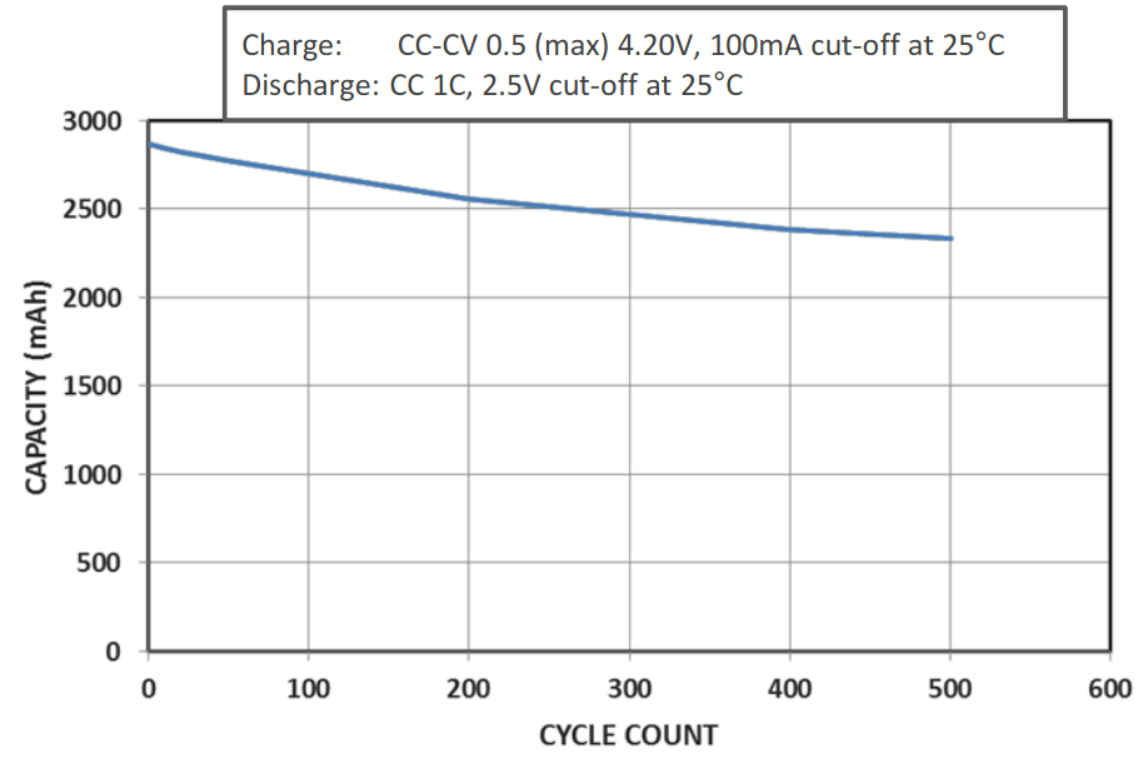
\includegraphics[width=0.4\textwidth]{life_cycle_18650.png}
	    \caption{Curva del ciclo de vida de una celda 18650}
        \label{life_cycle_18650}
	\end{subfigure}
    \end{centering}
    \caption{Curvas sgnificativas celda Panasonic 18650PF}
    \label{curvas_sign_18650}
\end{figure}

\newpage

\subsubsection{Ensamblado del pack}

El pack de bater\'ias es ensamblado utilizando soportes encastrables \emph{(Fig.
\ref{soporte_18650})} impresos utilizando una impresora 3D, donde cada celda es
conectada entre s\'i utilizando una banda de níquel y la conexi\'on es realizada 
por una soldadora de puntos manual. Esto es debido a dos motivos importantes, en 
primer instancia el tiempo en la aplicaci\'on de temperatura, por parte de la 
soldadura de puntos, es muy corto evitando problemas t\'ermicos de la celda 
durante el proceso de ensamblado. Por el otro lado, la banda de níquel tiene 
propiedades que benefician al ensamblado del pack, por ejemplo:

\begin{itemize}
    \item Protecci\'on en contra a la corrosi\'on.
    \item Buena conductividad el\'ectrica. El Niquel tiene la mitad de la
        resistencia el\'ectrica que el acero 1010.
    \item Buena resistencia mec\'anica.
    \item Bajo costo.
    \item Es soldable, por lo que se puede aplicar una soldadura de punto entre
        la tira de n'iquel y los electrodos de la celda.
\end{itemize}

\begin{figure}[h!]
    \begin{center}
        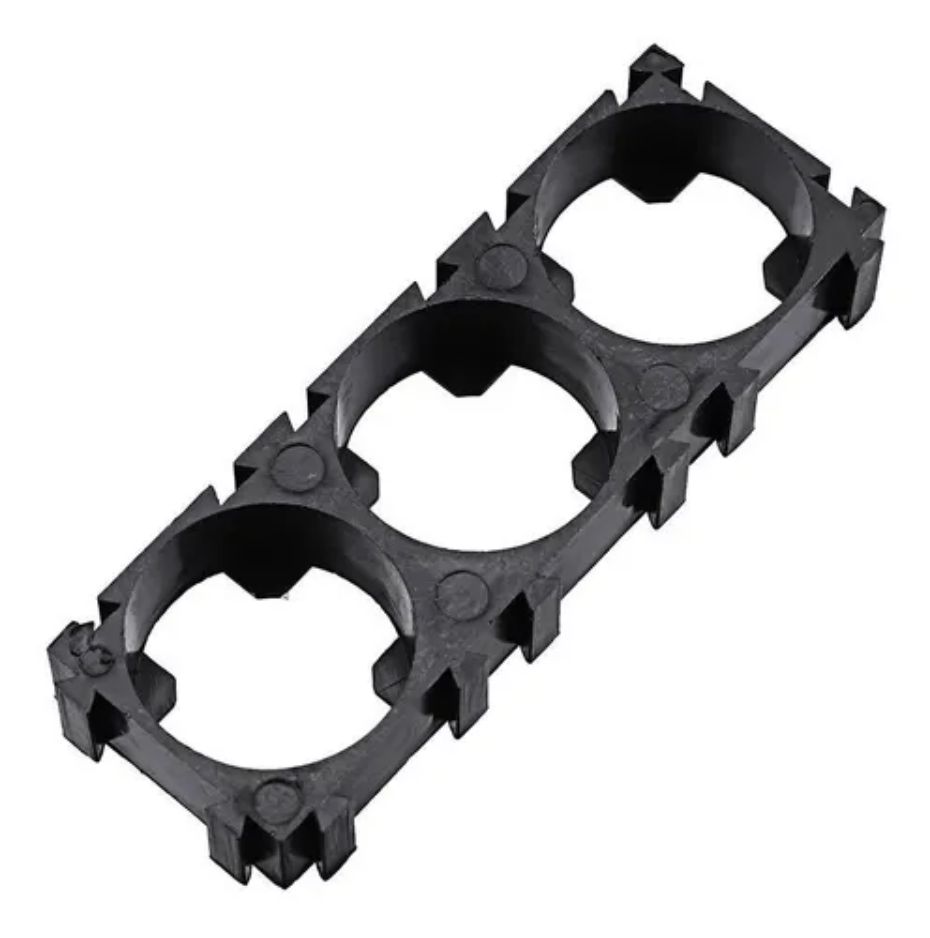
\includegraphics[width=0.45\textwidth]{soporte_18650.png}
        \caption{Soporte encastrable para celdas 18650}
        \label{soporte_18650}
    \end{center}
\end{figure}

Por el otro lado, a cada m\'odulo conectado en serie se le suelda un cable en
bornes de cada electrodo que va conectado a un conector JST-XH-2.50 para poder
acceder f\'acilmente al voltaje de cada m\'odulo del pack de bater\'ias. El pack
ensamblado se puede observar en las Figuras \ref{battery_top}-\ref{battery_side}

\begin{figure}[h!]
    \begin{subfigure}[b]{.3\textwidth}
	\begin{center}
        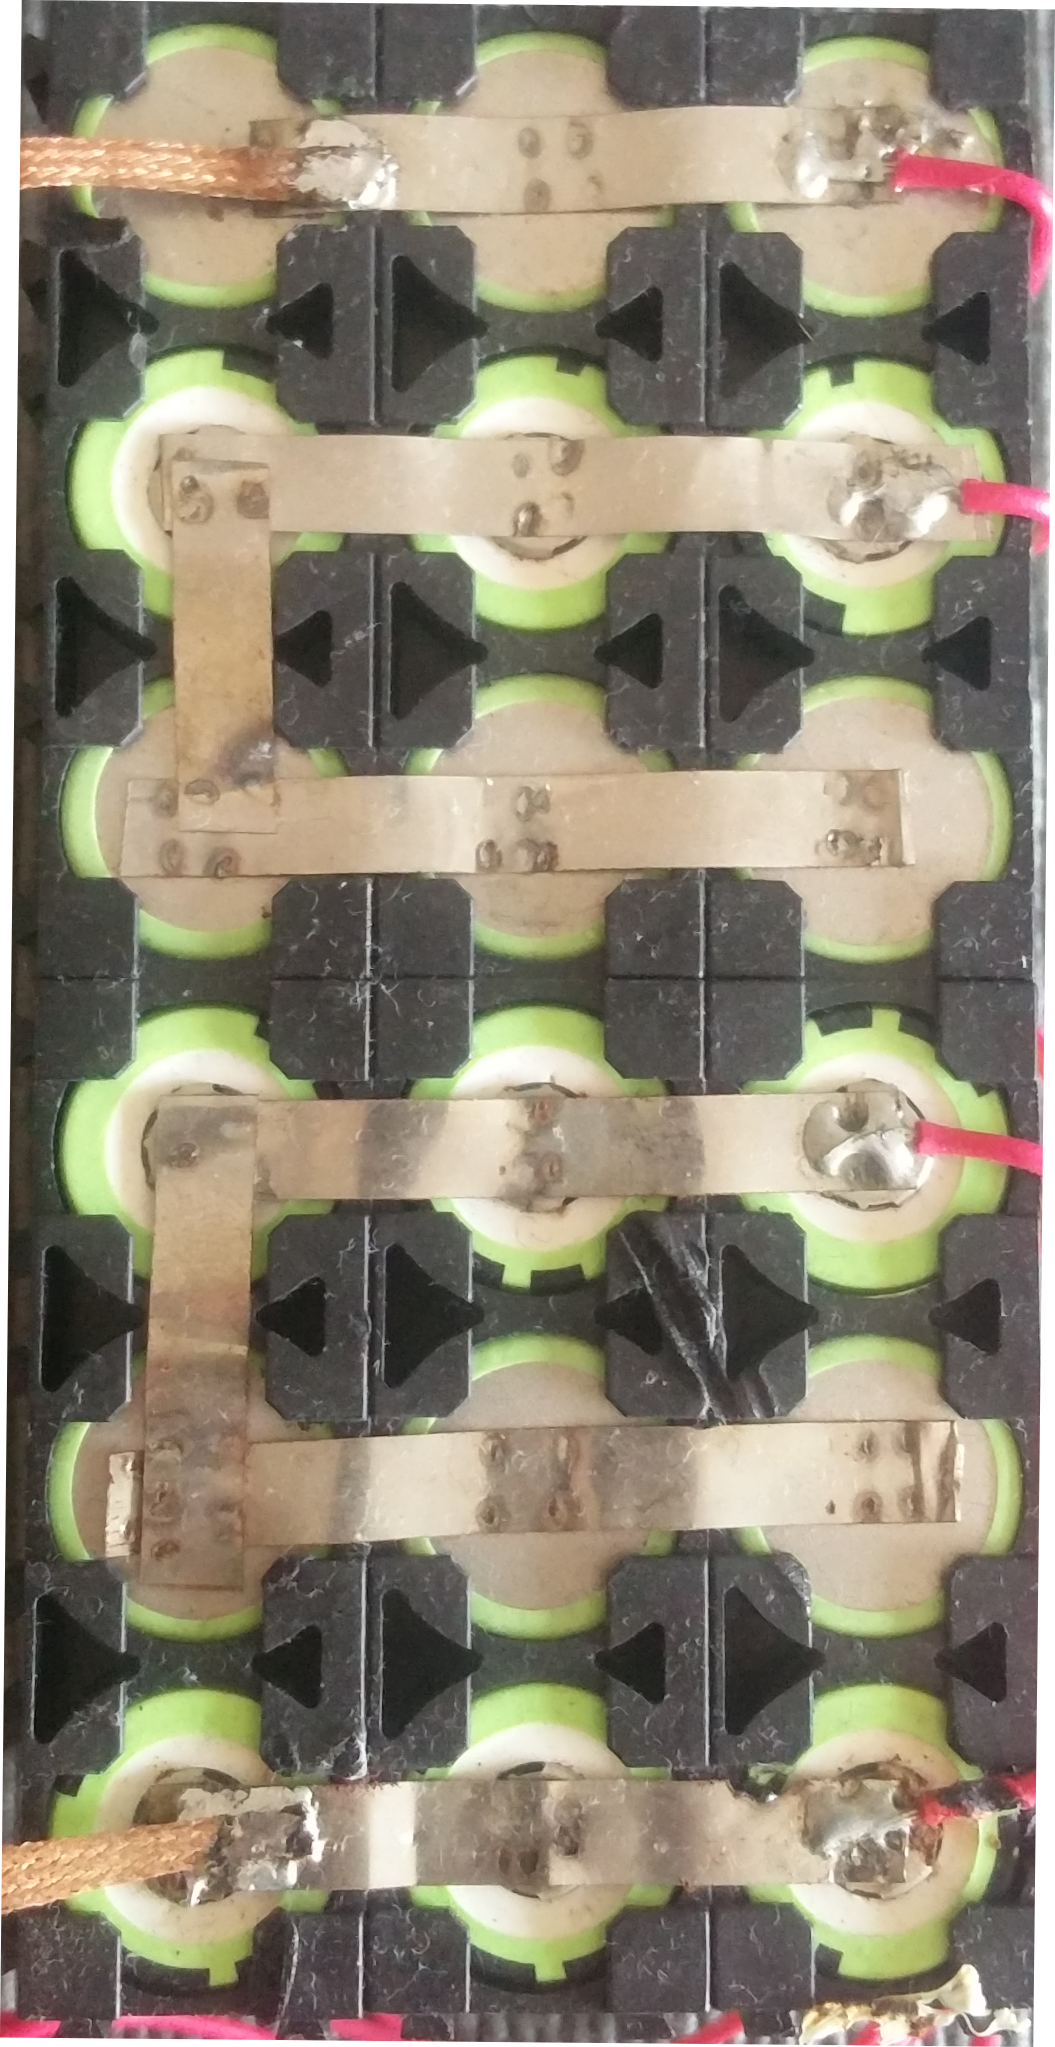
\includegraphics[width=.9\textwidth]{battery_top.png}
	\end{center}
    \caption{Imagen superior del pack de bater\'ias 6s3p. 
    }
	\label{battery_top}
    \end{subfigure}%
    \begin{subfigure}[b]{.3\textwidth}
	\centering
	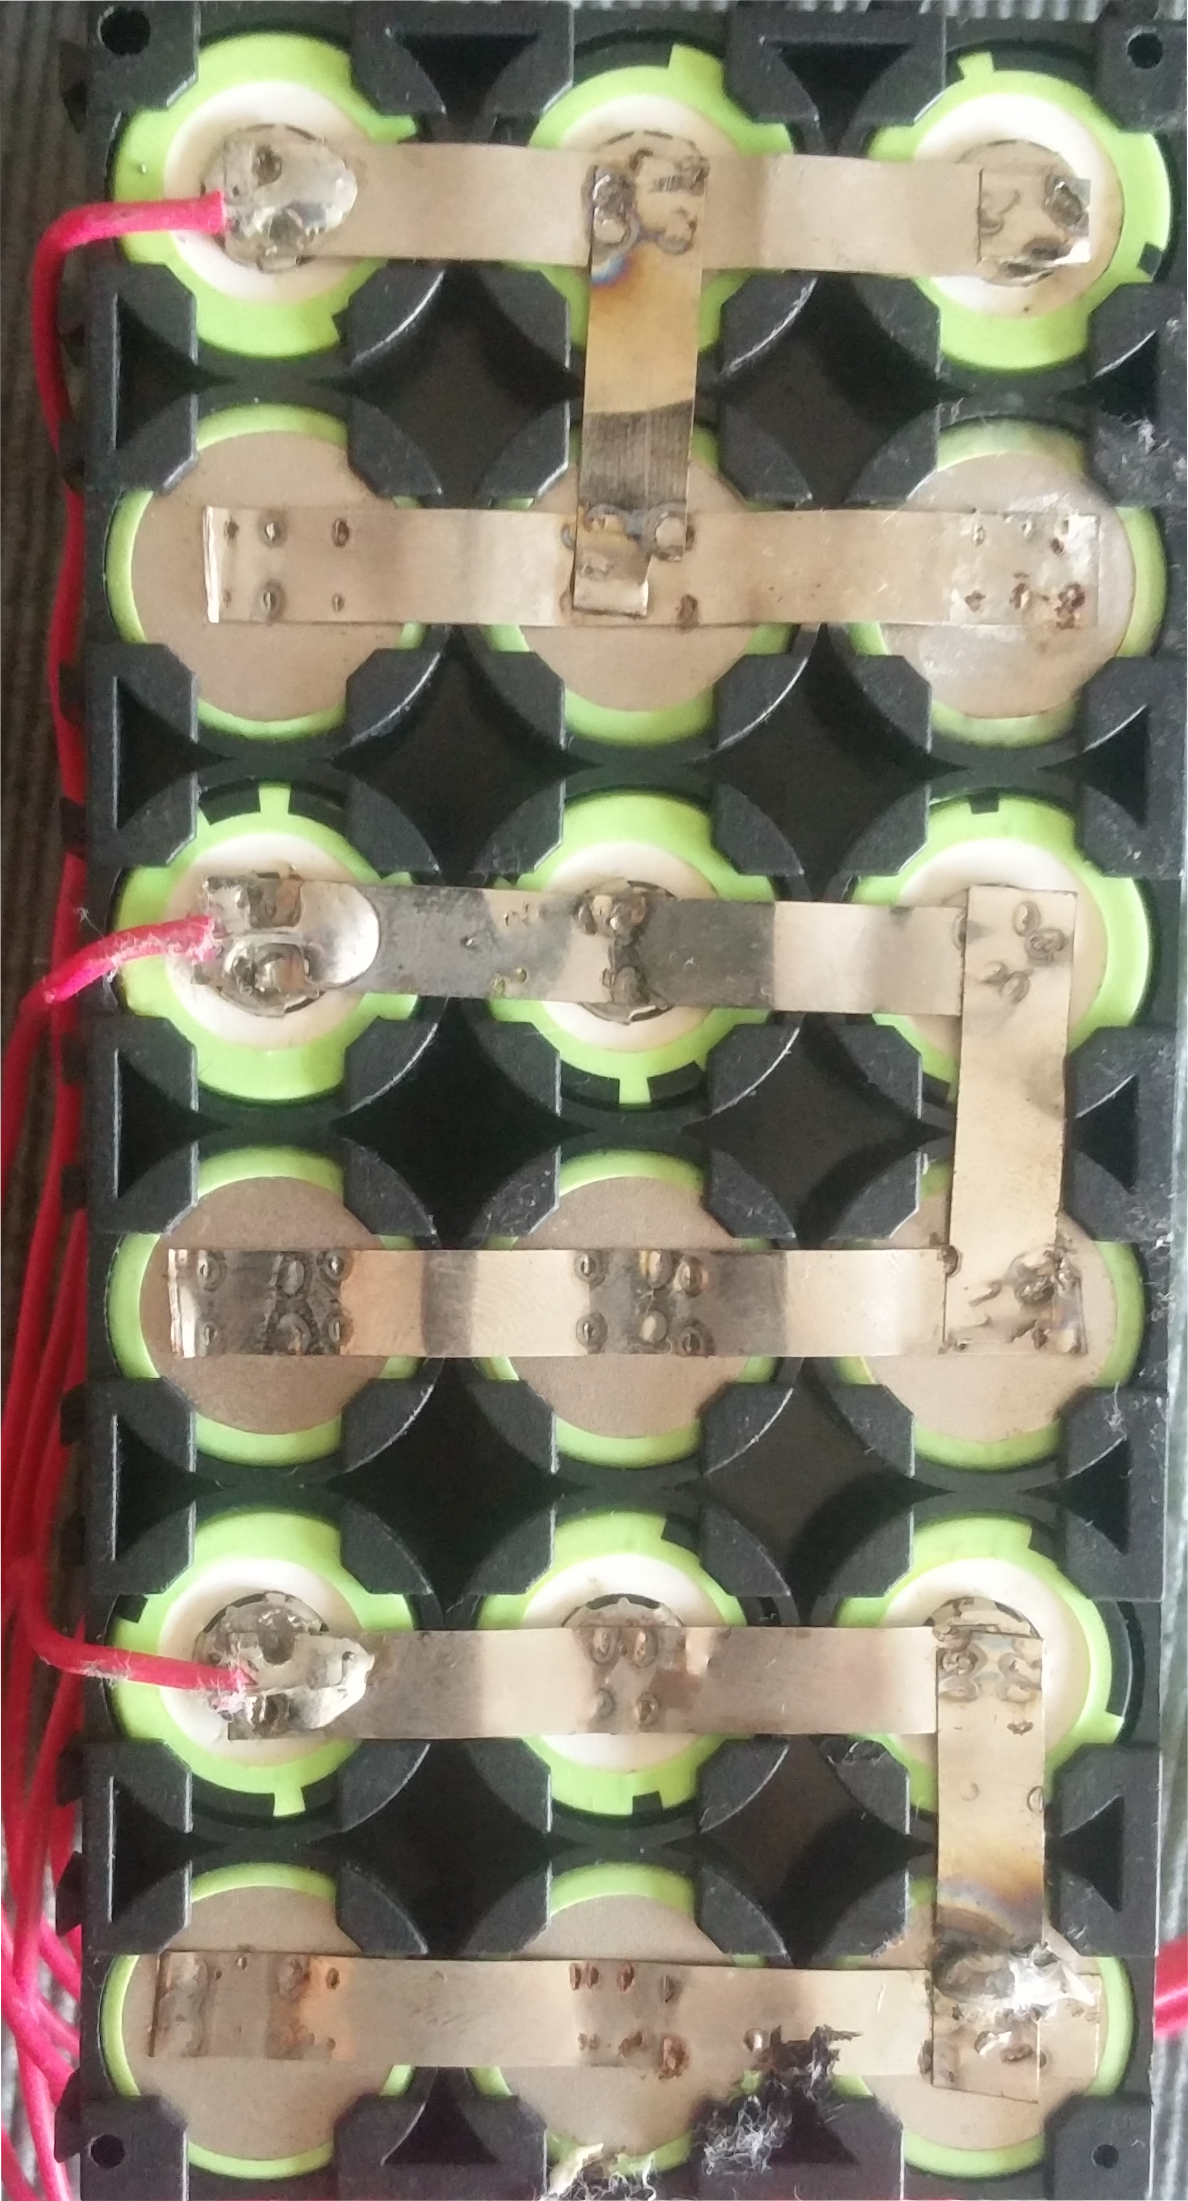
\includegraphics[width=.9\textwidth]{battery_bot.png}
	\caption{Imagen inferior del pack de bater\'ias 6s3p.}
	\label{battery_bot}
    \end{subfigure}
    \begin{subfigure}[b]{.3\textwidth}
	\centering
	\includegraphics[width=.9\textwidth]{batt_side.png}
	\caption{Imagen lateral del pack de bater\'ias 6s3p. En esta foto se puede
    apreciar el conector JST}
	\label{battery_side}
    \end{subfigure}
\end{figure}

\newpage

\subsubsection{Caracter\'isticas del pack}\label{caract_pack}

Como resultado obtenemos un pack de bater\'ias con las siguientes
caracter\'isticas:

\begin{itemize}
    \item Voltaje nominal de salida: 21.6V
    \item Voltaje m\'aximo de salida: 25.2V
    \item Voltaje m\'inimo de salida: 15V
    \item Capacidad t\'ipica: 8700mAh
    \item Capacidad m\'inima: 8250mAh
    \item Corriente de carga m\'axima: 4.35A
    \item Corriente de descarga m\'axima: 17.4A (2C)
\end{itemize}

\subsection{Modelo de la celda de litio-ion}\label{dev_batt_model}

Contar con un modelo matemático preciso que describa fehacientemente el
comportamiento y la dinámica de una celda de Ion-Litio es condición sine qua non
para la implementación exitosa de los algoritmos de estimación del
\acrshort{SOC} y de ecualización basados en el filtro de Kalman.

El modelado de una celda de litio puede ser abordado desde distintas
perspectivas y con difetentes herramientas matemáticas de acuerdo a los fines
que se persigan. La necesidad de conjugar un modelo de exactitud elevada que no
represente una carga computacional imposible de procesar en tiempo real en un
microcontrolador nos ha llevado a adoptar un modelo de segundo orden basado en
un circuito eléctrico siguiendo \cite{spagnol_kalman}, también conocido como
modelo de Randles de segundo orden, que se encuentra representado por el
esquem\'atico de la Figura \ref{randles_2rc} cuya parametrizaci\'on se describe
en la Secci\'on \ref{param_18650pf}.

\begin{figure}[h!]
    \begin{center}
	    \ctikzset{bipoles/length=1.0cm}
	    \ctikzset{bipoles/resistor/height=.3}

	    \begin{circuitikz}[american]
		\draw (0,0) to[R=$R_0$] (2,0) -- (2,-1) to[R=$R_1$] (4,-1) -- (4,0);
        \draw (2,0) -- (2, 1) to[C=$C_1$,v=$V_{C1}$] (4, 1) -- (4,0);
        \draw (4,0) to[short] (5, 0) -- (5, 1) to[C=$C_2$,v=$V_{C2}$] (7, 1) -- (7, 0);
		\draw (5,0) -- (5,-1) to[R=$R_2$] (7,-1) -- (7,0) to[short,f=$i$] (8,0);
        \draw (0,0) to[battery2=$V_{OCV}(SOC)$] (0,-3) -- (8,-3); 
        \draw  (8,0) to [open,v=$V_{out}$,invert] (8,-3);
	    \end{circuitikz}
        \caption{Circuito de Randles de Segundo Orden.}
        \label{randles_2rc}
    \end{center}
\end{figure}
\FloatBarrier

De acuerdo a la figura \ref{randles_2rc}, la salida del modelo es descripta por
la Ecuación \ref{eq:Vout_randles_2rc}

\begin{equation}
    V_{out}(t)=V_{OCV}(SOC)-(V_{R0}(t)+V_{C1}(t)+V_{C2}(t))
    \label{eq:Vout_randles_2rc}
\end{equation}

El modelo puede ser reescrito en el dominio de la transformada de Laplace como: 

\begin{align}
    \begin{split}
    V_{out}(t)&=V_{OCV}(SOC)-(R_{0}+\frac{R_{1}}{(1+sR_{1}C_{1})}\frac{R_{2}}{(1+sR_{2}C_{2})})i(t)\\
    &=V_{OCV}(SOC)-(R_{0}+\frac{K_{p}(1+sT_{2})}{(1+sT_{P1})(1+sT_{P2})})i(t)\\
    &=V_{OCV}(SOC)-R_{0}i(t)-G(s)i(t)
    \end{split}
       \label{eq:L_Vout_randles_2rc}
\end{align}

\subsubsection{Parametrizaci\'on del modelo}\label{param_18650pf}

La estimaci\'on de par\'ametros es com\'unmente usado para ajustar la respuesta 
de un modelo a los datos experimentales de un modelo f\'isico. En el caso de 
las celdas de litio-ion, los datos experimentales provienen de curvas
\acrfull{HPPC}. Este proceso involucra reiteradas simulaciones del modelo
matem\'atico planteado junto con la implementación y uso de un algoritmo de
optimizaci\'on num\'erico. De esta forma, el proceso de optimizaci\'on busca
ajustar los par\'ametros del modelo para minimizar el error entre los datos
experimentales y los resultados de las simulaciones realizadas.

En este caso, la curva \acrshort{HPPC}, que contiene un conjunto de pulsos de
carga/descarga, provee una representaci\'on con un alto nivel de fidelidad sobre
el comportamiento din\'amico de la bater\'ia, en m\'ultiples niveles del
\acrshort{SOC}. Para reflejar este comportamiento en el modelo planteado en la
Figura \ref{randles_2rc}, se requieren elementos circuitales no lineas flexibles
a las condiciones de operaci\'on y estados de la celda. Para realizar esto,
com\'unmente se emplean tablas de b\'usqueda (\acrshort{LUT}, del ingl\'es
\emph{\acrlong{LUT}}).

En este caso, los datos experimentales a analizar provienen de 
\cite{Kollmeyer2018}, que son descriptos en la siguiente secci\'on.

\subsubsection{Descripci\'on del set de datos}

El set de datos de  es un conjunto de ensayos realizados en 
la Universidad de Wisconsin-Madison por el Dr. Phillip Kollmeyer. Estos ensayos 
son realizados sobre una celda Panasonic NCR18650PF de 2.9Ah en una c\'amara 
t\'ermica con una celda de carga marca \emph{Digatron} que cuenta con una 
capacidad de descarga de 25A a 18V.

Los ensayos fueron realizados bajo 5 temperaturas diferents, en donde la
bater\'ia es cargada a 4.2V@2.9A despu\'es de cada ciclo. Sobre la celda se
ejecutaron los siguientes ciclos:

\begin{enumerate}
    \item 20 ciclos de Ensayo de carga y descarga.
    \item Cinco ensayos \acrshort{HPPC} a 0.5C, 1C, 2C, 4C y 6C realizados a
        intervalos de 5\% de \acrshort{SOC} en todo el rango de la capacidad de
        la celda.
    \item Ensayos \acrshort{EIS} en un rango de frecuencia de 1MHz a 100Hz, con
        el mismo paso y rango de \acrshort{SOC} que el punto anterior.
    \item Nueve ciclos de conducci\'on (del ing\'es, \emph{drive cycles})
        distintos, diseñados para poder capturar din\'amicas adicionales que no
        se pueden manifestar en el ensayo \acrshort{HPPC}.
    \item Los pasos 3 a 5 son ensayados nuevamente bajo 5 temperaturas distintas
        (25\degree C, 10\degree C, 0\degree C, -10\degree C y -20\degree C)
    \item Los nueve ciclos de conducci\'on se repiten con una temperatura
        inicial de -20\degree C, donde despu\'es se la permite evolucionar en
        funci\'on del calor generado por las bater\'ias.
    \item Los primeros 3 ciclos se repiten con la c\'amara a una temperatura
        inicial de -20\degree C.
    \item Los nueve ciclos de conducci\'on se ejecutan nuevamente con una
        temperatura inicial de 10\degree C.
    \item Los ciclos 1 a 4 se repiten con una temperatura inicial de 10\degree
        C.
    \item Finalmente, se le realizaron 10 ciclos de descarga a 1C con una
        temperatura ambiente de 25\degree C, seguidos por dos ensayos de
        referencia de capacidad demostrando que la capacidad m\'axima decae de
        2.8Ah a 2.3Ah despu\'es de correr todos los ensayos enumerados
        anteriormente.
\end{enumerate}

\subsubsubsection{Ensayos HPPC}\label{ensayo_HPPC}

El ensayo \acrshort{HPPC} es una metodología utilizada para poder caratcerizar
la dinámica de una celda. El perfil de ensayo \acrshort{HPPC} del dataset
\cite{Kollmeyer2018} presenta múltiples pulsos de descarga y de relajación a
intervalos de 5\% del estado de carga (\acrshort{SOC}). El ensayo es llevado a
cabo bajo el estricto control de la temperatura del electrolito y de la
corriente de descarga. Los pulsos de descarga son apreciablemente cortos
respecto del periodo de relajación siendo su duración de 1s y 2 minutos
respectivamente, con la intención de que el pulso del ensayo perturve la celda
sin modificar su estado de carga.

Para poder poblar las tablas de busqueda del modelo es necesario contar con
información experimental suficiente que ejercite cada uno de los parámetros que
las componen. Son las curvas del ensayo \acrshort{HPPC}, que pueden observarse
en la Figura \ref{hppc_kollmeyer}, las que nos brindan la imformación necesaria.

\begin{figure}[h!]
    \begin{center}
        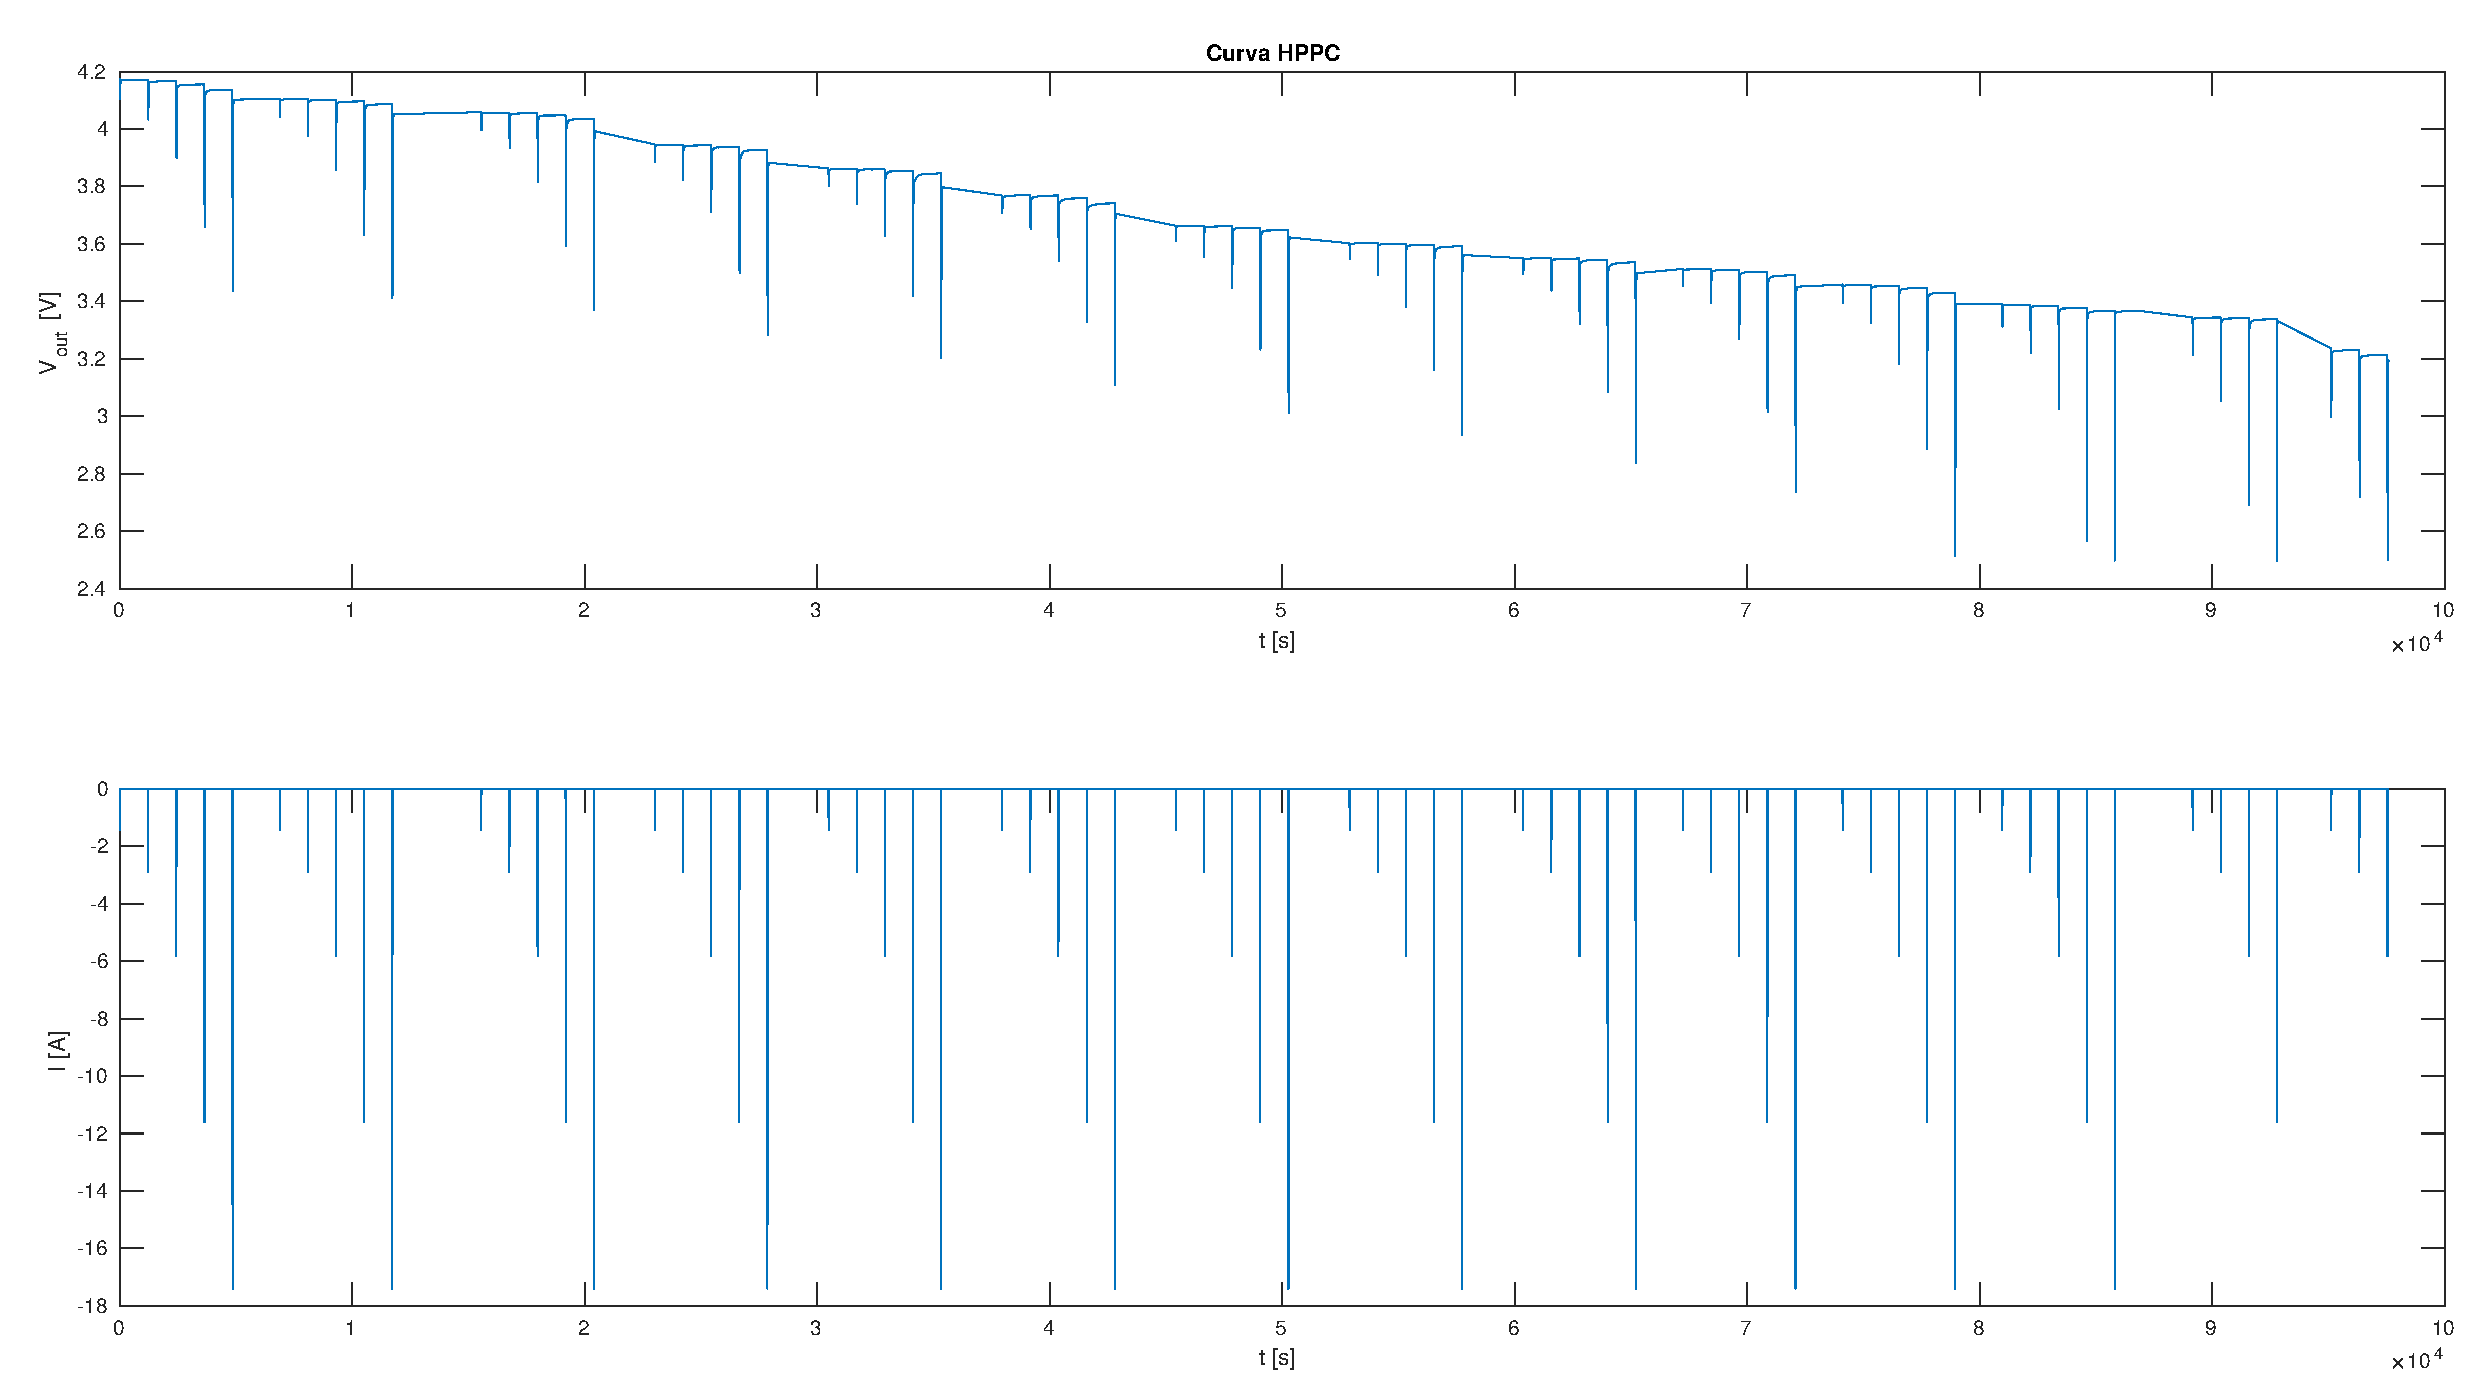
\includegraphics[width=.9\textwidth]{hppc_kollmeyer.eps}
        \caption{Curva HPPC provista por \cite{Kollmeyer2018}}
        \label{hppc_kollmeyer}
    \end{center}
\end{figure}
\FloatBarrier

%\newpage

La Figura \ref{hppc_kollmeyer_zoom} muestra una vista detallada y ampliada de
uno de los pulsos de descarga que conforman el ensayo \acrshort{HPPC}. Cada uno
de estos pulsos nos brindan no solo información respecto de la tensión de
circuito abierto (\acrshort{OCV}), sino tambien de la evolución de la celda
frente a una excitación por corriente a estados de carga (\acrshort{SOC})
determinado.

\begin{figure}[h!]
    \begin{center}
        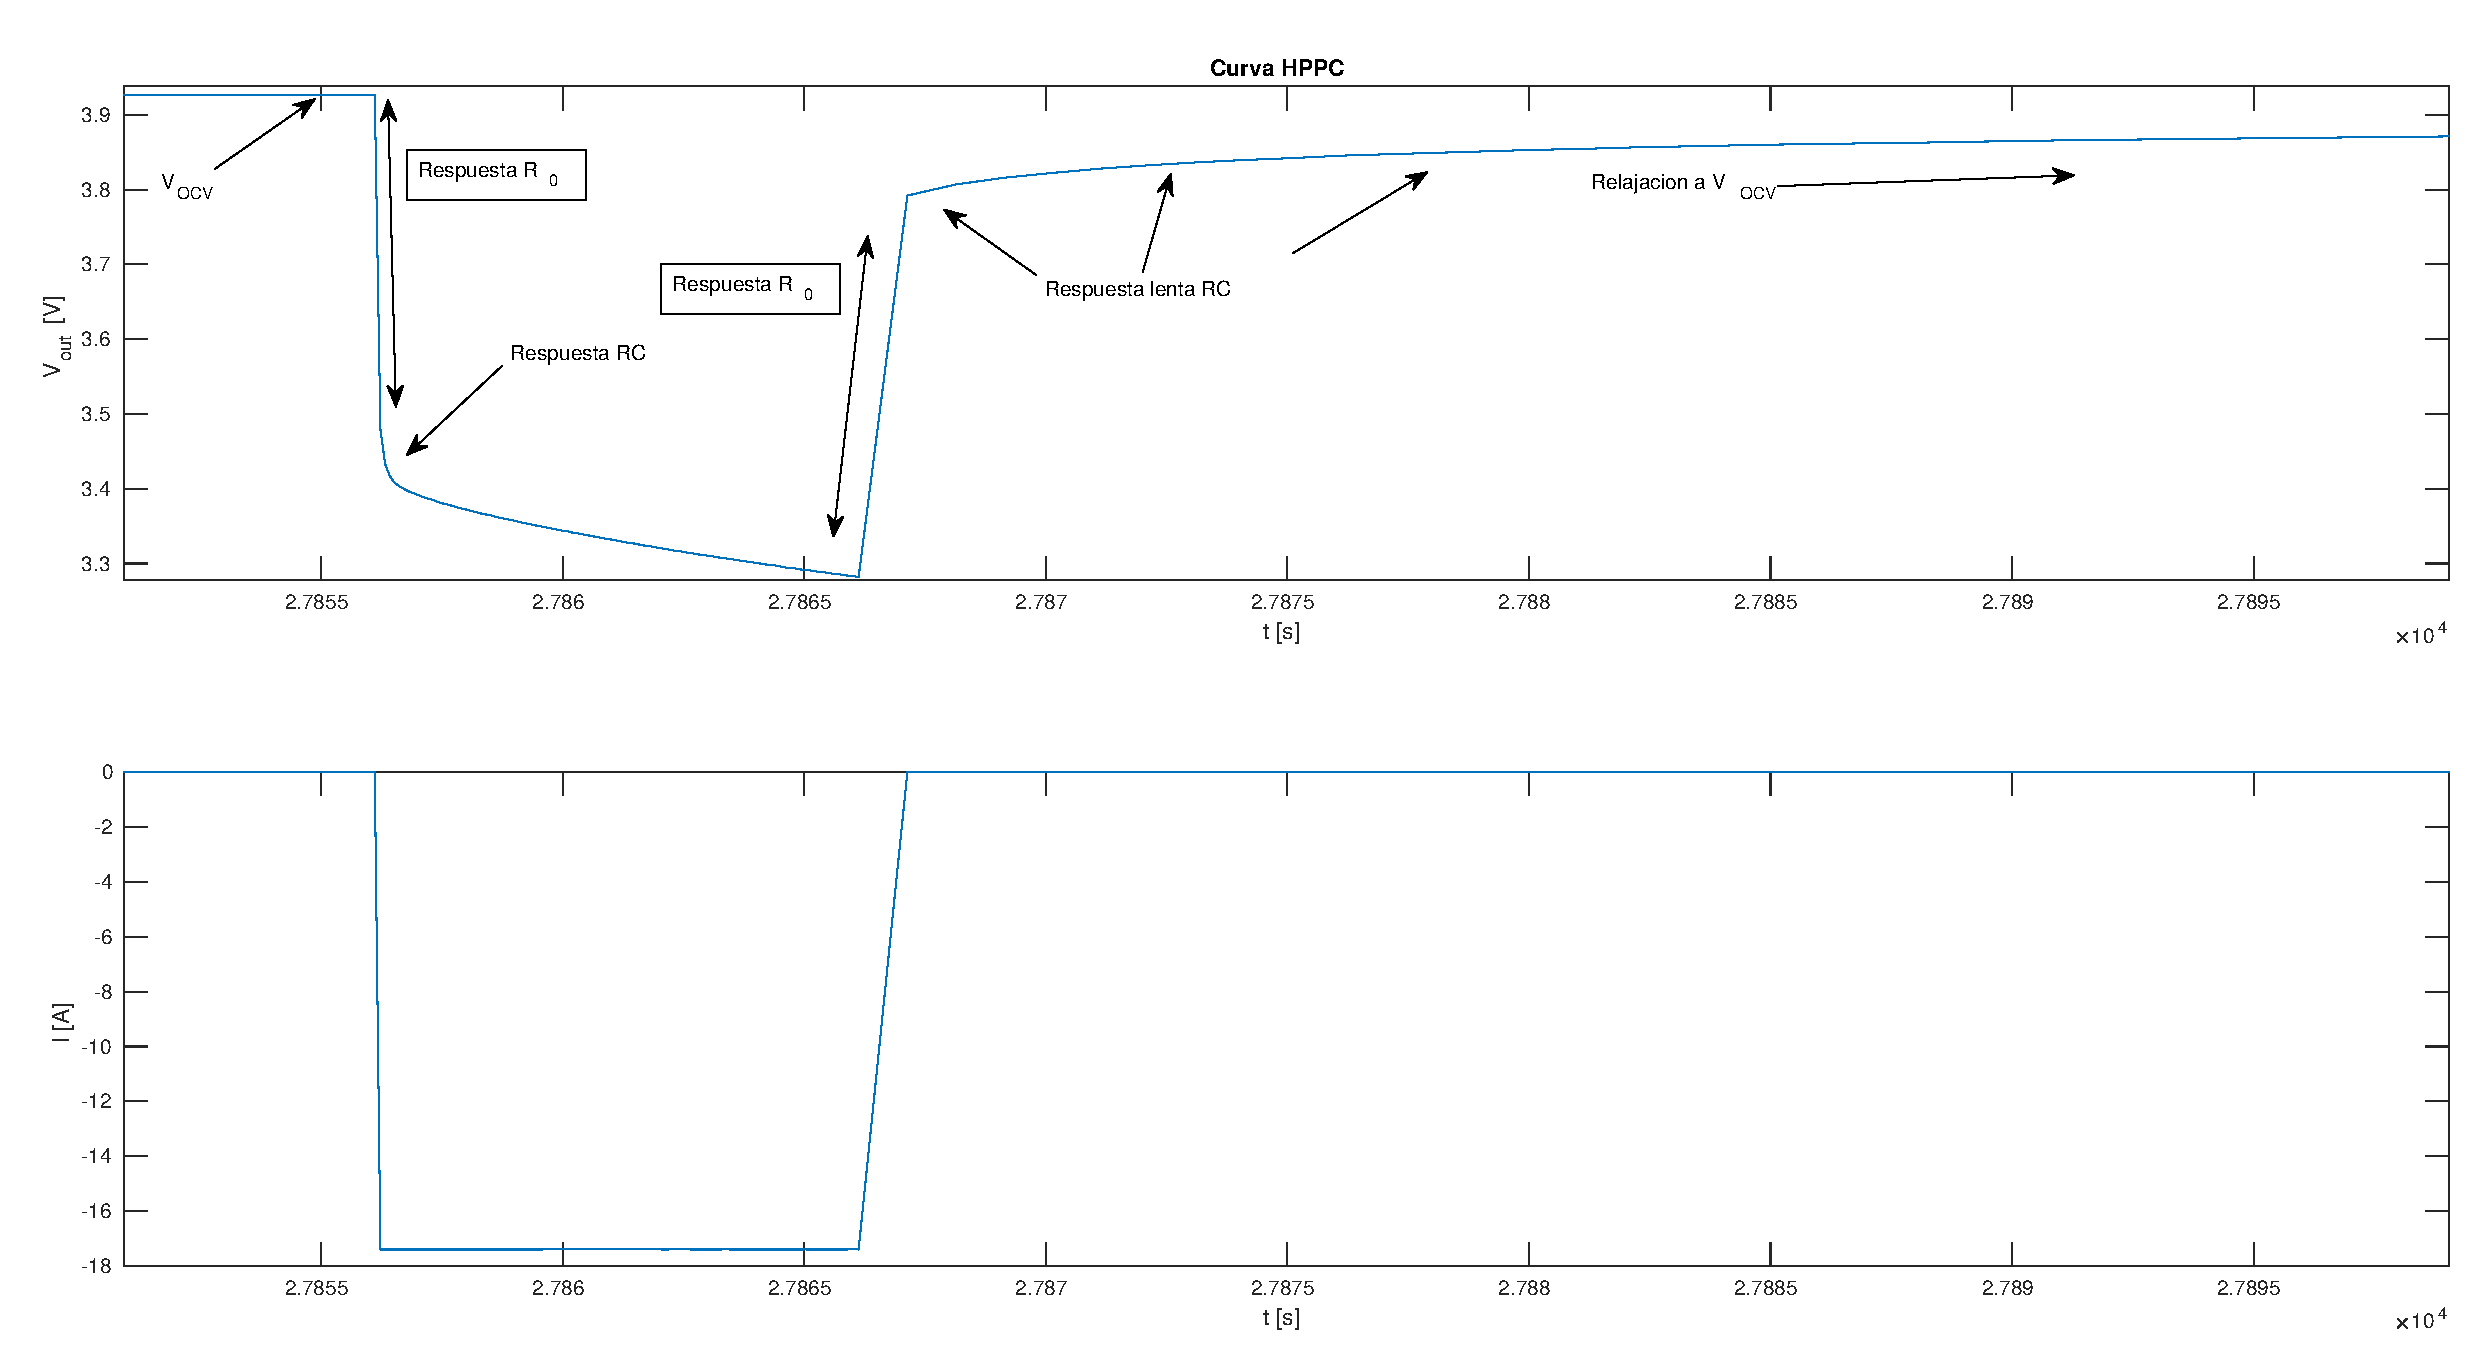
\includegraphics[width=.9\textwidth]{hppc_kollmeyer_zoom.eps}
        \caption{Ampliaci\'on sobre un pulso de la curva HPPC provista por 
                 \cite{Kollmeyer2018}}
        \label{hppc_kollmeyer_zoom}
    \end{center}
\end{figure}
\FloatBarrier

\subsubsection{Validación número de ramas R-C del modelo}

Para validar que el modelo propuesto sea capaz de describir la dinámida completa
de una celda de Ion-Litio ensayada se ajustaron 2 ecuasiones exponenciales, una
de orden 1 (Eq. \ref{eq:exp1}) y otra de orden 2 (Eq. \ref{eq:exp2}), a la curva
que traza los datos del en sayo HPPC utilizando la herramienta Curve Fitting de
Matlab.

\begin{align}
    Y &= a*exp(b*x)\label{eq:exp1}\\
    Y &= a*exp(b*x)+c*exp(d*x)\label{eq:exp2}
\end{align}

Se selecciono especificamente la fase de relajación de uno de los escalones del
ensayo HPPC. Cuando se retira el escalón de corriente, la respuesta transitoria
inmediata es condicionada por $R_{0}$ pero rapidamente la dinamica
fundamentalmente es descipta por el número de ramas R-C en serie dispuestas en
el circuito equivalente. 

\begin{figure}[h!]
    \begin{center}
        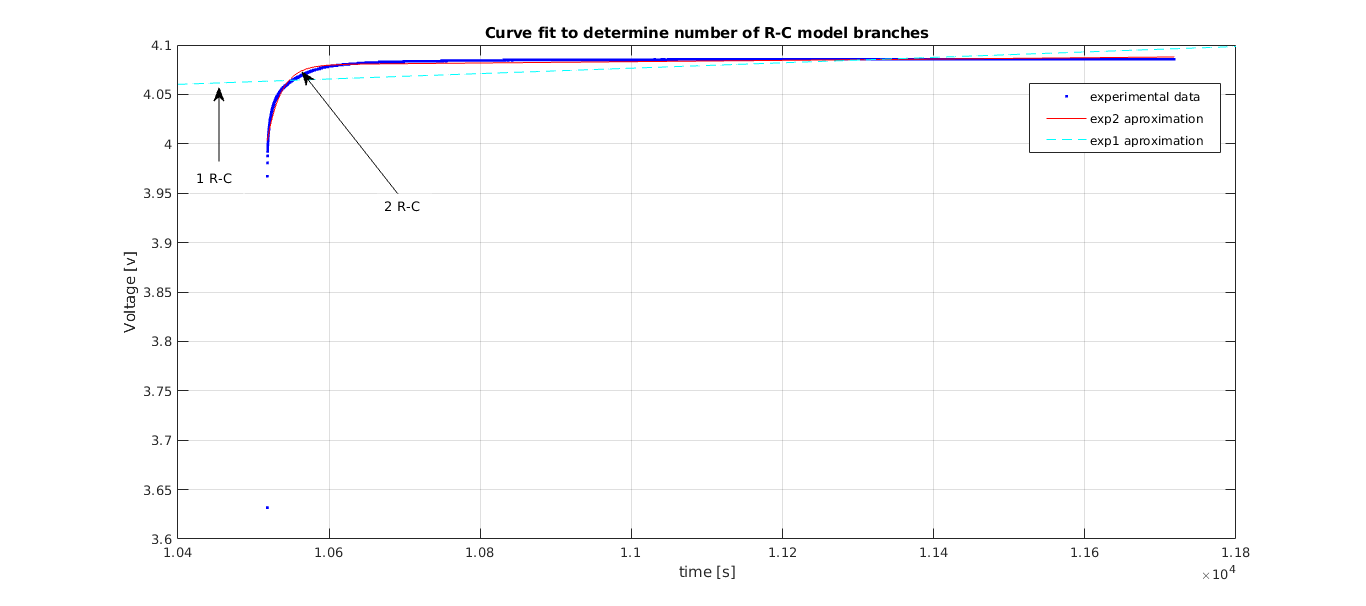
\includegraphics[width=.65\textwidth]{rc_model_fit.png}
        \caption{Ajuste curvas exponenciales orden Modelo R-C}
        \label{fig:model_fit}
    \end{center}
\end{figure}
\FloatBarrier

A la vista del resultado obtenido en la Figura \ref{fig:model_fit} se concluye
que 2 terminos exponenciales temporales serán suficientes para describir la
dinamica de una celda de Ion-Litio ensayada. Situación de compromiso entre
la precisión del modelo, la complejidad matemática y la necesidad de mantener el
costo computacional bajo a los fines de embeber el modelo en el
microcontrolador. 

\subsubsection{Implementación del circuito de Randles}

Para llevar a cabo el proceso de estimación y optimizaci\'on de par\'ametros, en
primer instancia se necesita implementar el circuito de Randles en un ambiente
de simulaci\'on. En este caso, el modelo fue desarrollado en \emph{Simulink}
utilizando la librer\'ia \emph{Power Systems} de \emph{Simscape} para crear a
medida y representar los elementos pasivos que lo componen y las señales de
entrada y salida.

El modelo est\'a compuesto por una fuente de tensi\'on controlada, que
representa el \acrshort{OCV} de la bater\'ia y 5 \acrshort{LUT}s que
representan los componentes pasivos del circuito. Los 6 componentes depende
exclusivamente del nivel de \acrshort{SOC} de la bater\'ia. Su implementaci\'on
se puede observar en la Figura \ref{battery_model_simulink}. 

El modelo implementado, a su vez, incluye una fuente de corriente a la salida
que hace las veces de carga de la celda y logra capturar la señal de corriente
proveniente del set de datos.

\begin{figure}[h!]
    \begin{center}
        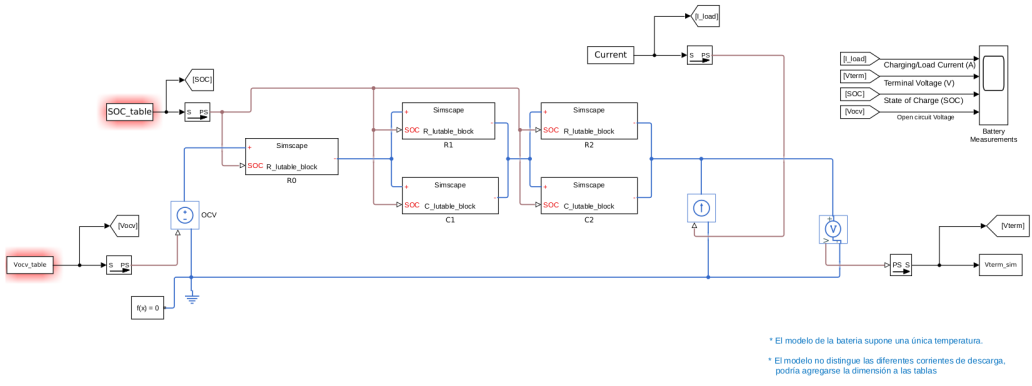
\includegraphics[width=.9\textwidth]{battery_model_simulink.png}
        \caption{Implementaci\'on del modelo de Randles en \emph{Simulink}.}
        \label{battery_model_simulink}
    \end{center}
\end{figure}
\FloatBarrier

Las variables de entrada del modelo serán entonces: 

\begin{itemize}
    \item $SOC(t)$
    \item $V_{OCV}(SOC)$
    \item $I_{load}(t)$
\end{itemize}

El modelo nos permite observar la evolucíon de la tensión en bornes de la celda
ante las variaciones de sus variables de entrada a partir de la medición de la
tensi\'on de salida que simula el mismo.

El modelado de los componentes a partir de \acrshort{LUT} no contempla
variaciones de temperatura del electrolito de la celda ni de la corriente
circulante por los elementos. Como condición de diseño se supone que el valor de
los elementos posivos no se ve modificado ante la variación de la corriente de
excitación de los mismo. Diferentes condiciones de operación, tanto en
temperatura como en corriente de excitación, requeriran simplemente repetir el
proceso de simulación para cada particularidad poblándose las nuevas dimensiones
obtenidas de la \acrshort{LUT} de forma manual.

Se valida el funcionamiento de la implementación del modelo propuesto para
representar el set de datos disponible observando la respuesta del mismo ante la
excitacipon con un escal\'on de corriente.

\newpage

Para el ensayo se utilizan par\'ametros con valores predeterminados: 

\begin{itemize}
    \item $C_{1} = C_{2} = 1F$
    \item $ R_{1} = R_{2} = 1m\mathrm{\Omega}$
    \item $\mathrm{R_0}=40m\mathrm{\Omega}$
\end{itemize}

\begin{figure}[h!]
    \begin{center}
        \includegraphics[width=0.8\textwidth]{v_sim_v_dataset_no_opt.eps}
        \caption{Comparaci\'on de la tensi\'on de salida del modelo de
                 \emph{Simulink} sin optimizar con la curva de tensi\'on de 
                 salida del set de datos}
         \label{comp_simulink_no_opt}
    \end{center}
\end{figure}
%\FloatBarrier

Se puede observar en la Figura \ref{comp_simulink_no_opt} que a pesar de no
estar optimizados los parámetros para disminuir el error en la tensi\'on de
salida, el modelo logra representar, de forma lejana, la din\'amica de la
respuesta al escal\'on validando la implementación realizada.

%\newpage

\subsubsection{Pre-procesamiento datos}\label{data_preprocessing}

El conjunto de datos del ensayo \acrshort{HPPC} de \cite{Kollmeyer2018} debe ser
preprocesado para obtener ciertas variables de inter\'es, como por ejemplo, la
señal del \acrshort{SOC} de la curva relevante para comparar los resultados de
nuestro modelo, como tambi\'en la segmentaci\'on o modificaci\'on de los datos
es \'util para el desarrollo del modelo.

\subsubsubsection{Curva de \acrshort{SOC}}

Dentro de los datos de la curva \acrshort{HPPC}, el ensayo de
\cite{Kollmeyer2018} acumula la corriente que circula desde y hacia el pack en
Ampehere-hora (Ah), en base a esto, se calcula \acrshort{SOC} en todo el ensayo
usando la Ecuaci\'on \ref{calculo_soc_ah}.

\begin{equation}
    SOC = \frac{Ah_{acumulado} + Ah_{min}}{Ah_{min}} \label{calculo_soc_ah}
\end{equation}

Implementando la Ecuaci\'on \ref{calculo_soc_ah} en Matlab sobre la curva Ah del
ensayo \acrshort{HPPC} se obtiene la gr\'afica que se observa en la Figura
\ref{soc_hppc_data}.

\begin{figure}[h!]
    \begin{center}
        \includegraphics[width=0.8\textwidth]{soc_hppc_data.eps}
        \caption{Curva del \acrshort{SOC} para el ensayo HPPC de
        \cite{Kollmeyer2018}. En el mismo se pueden observar los escalones de
        \acrshort{SOC} generados por los pulsos de corriente aplicados en la
        celda.}
        \label{soc_hppc_data}
    \end{center}
\end{figure}
\FloatBarrier

\subsubsubsection{Obtenci\'on del \acrshort{OCV}}

Dentro de la curva \acrshort{HPPC} de la Figura \ref{hppc_kollmeyer}, podemos
observar per\'iodos de descanso lo suficientemente largos como para considerar
que la bater\'ia alcanz\'o la estabilidad qu\'imica, por lo tanto, presentando
una lectura de voltaje equivalente al \acrshort{OCV}. Esta informaci\'on del 
\acrshort{OCV} durante el ensayo, permite relacionar la tensi\'on de circuito 
abierto de la celda con el estado de carga para los distintos pulsos de la 
curva. \'Esta variable resulta de gran importancia para parametrizar y ajustar
los distintos par\'ametros del modelo, porque representa la fuente de voltaje
controlada por el \acrshort{SOC} de la Figura \ref{randles_2rc}.

Para construir la curva de \acrshort{OCV}, se retuvieron los valores de voltaje
en los puntos donde se detect\'o un flanco negativo, como se describe en la
Secci\'on \ref{flank_seg} y se extrapoló este valor hasta el siguiente flanco
negativo, obteniendo la curva de la Figura \ref{fig:ocv_detection}.

\begin{figure}[h!]
    \begin{center}
        \includegraphics[width=.7\textwidth]{soc_detection}
        \caption{En naranja se muestra el \acrshort{OCV} en la que se observa
        que toma el mismo valor de voltaje antes de que ocurra el flanco
        negativo en la celda, y en azul la curva \acrshort{HPPC} original}
        \label{fig:ocv_detection}
    \end{center}
\end{figure}
\FloatBarrier

\newpage

Relacionando estos resultados con los datos obtenidos en la Figura 
\ref{soc_hppc_data}, obtenemos la curva que representa la fuente de voltaje
controlada por \acrshort{OCV} del esquem\'atico en la Figura \ref{randles_2rc}.
Esta curva se puede observar en la Figura \ref{fig:ocv_vs_soc}.

\begin{figure}[h!]
    \begin{center}
        \includegraphics[width=.7\textwidth]{ocv_vs_soc.eps}
        \caption{Curva \acrshort{OCV} en relaci\'on al \acrshort{SOC}, que
            representa el funcionamiento de la fuente de voltaje controlada por
        \acrshort{SOC} en el esquem\'atico de Randles.}
        \label{fig:ocv_vs_soc}
    \end{center}
\end{figure}
\FloatBarrier

\subsubsubsection{Segmentaci\'on de Datos}\label{flank_seg}

El número de tanques R-C que conforman el modelo y consecuentemente el de
parametros a estimar, unos 67 juegos de 5 parámetros cada uno, junto con el
tamaño del dataset del ensayo \acrshort{HPPC} que se observa en la Figura
\ref{hppc_kollmeyer} plantean el desafío computacional que significa la
estimación y optimización de los mismos. 

Son parámetros a tener en cuenta la velocidad de cómputo y el consumo de
memoria, la selección de las condiciones iniciales, seteos y condiciones de
borde de los parámetros a calcular que implican una etapa de
prueva y error hasta obtener un proceso funcional acorde a los resultados
deseados y el tiempo de programación que ello implica.

Como resultado de las complejidades planteadas y en vista de evaluar el resultado
del proceso de optimizaci\'on del modelo en toda la extensión de la curva
\acrshort{HPPC}, es necesario segmentar los datos disponibles en porciones que
sean faciles de abordar. Idealmente los datos del ensayo fueron separados según
los pulsos de corriente para cada nivel del \acrshort{SOC}. 

Para ello se implementa en MATLAB un algoritmo llamado \texttt{flanks.m}, el cual
dado un arreglo de valores y un porcentaje espec\'ifico compara las muestras
entre dos instantes contiguos [n, n+1]. Si la diferencia entre ambas muestras es
mayor al porcentaje especificado de un flanco ascendente marca ese instante con
un 1, si es mayor al porcentaje anterior de un flanco descendiente marca ese
instante con -1, caso contrario, marca ese instance con un 0. Esto permite
identificar los instantes de tiempo en los que se genera un pulso de
corriente/tensi\'on de la bater\'ia para poder segmentar el conjunto de datos y
post-procesarlo para optimizar el modelo. Las \acrshort{LUT}s tendrán los saltos
en los mismos intervalos.

El resultado del algoritmo se puede observar a partir de uno de los pulsos de
corriente de la curva \acrshort{HPPC} a modo de ejemplo de su funcionamiento en
la Figura \ref{flank_seg_hppc}

\begin{figure}[h!]
    \begin{center}
        \includegraphics[width=.8\textwidth]{flank_seg_hppc.eps}
        \caption{Identificación segmentos curva
        \acrshort{HPPC}, se puede observar los picos 1 y -1 indicando los
        instantes en los que comienza y finaliza un pulso de corriente}
        \label{flank_seg_hppc}
    \end{center}
\end{figure}
\FloatBarrier

Una vez identificados todos los flancos segmentamos el set de datos en porciones
abarcables por el algoritmo de optimización. En la Imagen
\ref{fig:data_seg_hppc} se puede apreciar, a modo de ejemplo, la porción de
datos seleccionada y el criterio de corte utilizado. Para cada uno de los ciclos
de optimización se seleccionó el intervalo de datos comprendidos entre dos
flancos consecutivos descendentes. Puede notarse el solapamiento entre los
intervalos de datos seleccionados teniendo en cuenta los puntos donde se tomó el
\acrshort{SOC} para definir los cortes de la \acrshort{LUT}s. Esto permite que
el algoritmo cuente con la información suficiente para ejercitar todos y cada
uno de los parámetros del modelo.

\begin{figure}[h!]
    \centering
        \includegraphics[width=1\textwidth]{data_seg_hppc.png}
        \caption{Segmento n - Dataset ensayo \acrshort{HPPC}}
        \label{fig:data_seg_hppc}
\end{figure}
\FloatBarrier

La posibilidad de extender o acortar los puntos de inicio y fin de la trama de
datos otorga un grado más de libertad. Dependiendo de cada ciclo de
optimización, puede ser de utilidad retener el principio del pulso siguiente
debido a que los valores de los parámetros del pulso anterior son tambien
ejercitados al principio del intervalo siguiente. 

Cada pulso de corriente y su respectiva contraparte en tensión se pueden dividir
en 2 zonas, una de excitación, aquella donde la corriente forzada está
circulando por le modelo y una zona de relajación a partir de que el pulso de
corriente es eliminado. La zona de excitación puede ser considerada como una
zona de transición entre \acrshort{SOC}s y entradas de las \acrshort{LUT}s.
Es la zona de relajación la que cuenta con la mayor información sobre de la
dinámica del sistema para ejercitar cada parámetro del modelo incluido el cambio
instantaneo de voltaje que representa $R_{0}$. La zona de excitación no 
brinda información sobre la dinámica completa del sistema, solo nos
brinda información parcial, fundamentalmente sobre la parte rápida de la
dinámica. 

\subsubsection{Algoritmo recursivo de optimizaci\'on}

El proceso de estimación y ajuste de los parámetros del modelo se realizó a
partir de la implemenación en MATLAB de un algoritmo recursivo de optimización
que ejecuta la tarea de cálculo y ajuste de cada uno de los juegos de parámetros
correspondientes a los segmentos de datos del ensayo \acrshort{HPPC} seccionados
en el pre-procesamiento de forma secuencial y automatizada.

El algoritmo desarrollado e implementado en \texttt{Semi-Automatic Li Ion
battery RC model parameters estimator.m} se repite automaticamente para cada
sección de datos seleccionada del ensayo \acrshort{HPPC} procesando cada una de
las tareas de estimación y optimización secuencialmente. El código selecciona
una porción de datos, setea los parámetros a ser estimados aplicando las
condiciones iniciales y de limites de los mismos. El codigo a su vez prepara el
modelo para ser ejecutado en cada tarea de estimación y ajuste seleccionando los
intervalos correctos de las señales de entrada del modelo y sus condiciones
iniciales.

Los límites de los parámetros a estimar se setean de forma experimental tomando
en cuentas los resultados de cálculos matematicos realizados previamente y de
algunos ciclos de optimización ejecutados a los fines de la puesta a punto del
sistema. Los valores obtenidos se definen a continuación. 

\begin{itemize}
    \item [] $ 0 < \mathbf{R_0} < 1$
    \item [] $ 0 < \mathbf{R_1} < 1$ $ 0 < \mathbf{C_1} < 200$
    \item [] $ 0 < \mathbf{R_2} < 1$ $ 0 < \mathbf{C_2} < 3000$
\end{itemize}
\FloatBarrier

Una vez que se encuentra corriendo la tarea de optimización, la implementación
ejecuta un algoritmo automatizado de optimización numérica a partir de la
herramienta de Estimación de Parametros, parte del toolbox \emph{Design
Optimization} de \emph{Simulink} que provee de funciones, herramientas activas
y bloques para el tratamiento de modelos. El toolboox provee de la capaciad de
interacción entre el modelo de la celda desarrollados con la librer\'ia
\emph{Power Systems} de \emph{Simscape}, la información experimental del ensayo
\acrshort{HPPC} proveniente del dataset y el algoritmo de optimización planteado.

El método matematico de optimización seleccionado es el de mínimos cuadrados no
lineales implementado a partir de la función \emph{lsqnonlin} del toolbox de
optimización. 
El método minimiza los cuadrados de los residuos, por lo que requiere ser
provisto de un vector de errores residuales, particular de nuestra solución, el
cual se computa sobre una base de tiempo fija.
El solucionador de mínimos cuadrados no lineales resuelve problemas de ajuste de
curva de mínimos cuadrados no lineales de la forma

\begin{equation}
    \min_{x}\|f(x)\| = \min_{x} (f_1(x)^2 + f_2(x)^2+\dots+f_n(x)^2)
\end{equation}

El vector de errores residuales se implementa en
\texttt{sdoVtermEstimation\_Objective.m}. La función es provista al optimizador y
utilizada para simular y comparar la salida obtenida del modelo respecto de los
datos experimentales provistos. Los argumentos devueltos por la función
contienen imformación respecto de como se ajustan los resultados de la
simulación $y_{s}(t)$ a los datos experimentales $y_{r}(t)$ en todos los puntos
simulados de la forma observada en la Ecuación \ref{eq:residual}.

\begin{equation}
    e(t) = y_{s}(t)–y_{r}(t) 
    \label{eq:residual}
\end{equation}

La función devuelve un vector de valores y no la suma de los cuadrados de los
valores. El algoritmo de optimización calcula implícitamente la suma de los
cuadrados de las componentes de $F(x)$ del vector de errores devuelto de la
forma vista en la Ecuación \ref{eq:residual_vect}.

\begin{equation}
    F(x) = \begin{bmatrix}
        e(0)\\
        \vdots\\
        e(N)\\
    \end{bmatrix}
    \label{eq:residual_vect}
\end{equation}

La selección del método de optimización fue realizada a instancias de
\cite{Jackey2013BatteryMP} y debido a que el método \emph{lsqnonlin} es
computacionalmente varias veces más rápido en comparación a otros metodos para
la solución del problema en cuestión.

El proceso de optimización se completa una vez que el tamaño del gradiente del
vector residual es menor que el valor de tolerancia de optimización
seleccionado.

\begin{figure}[h!]
	\begin{center}
		\includegraphics[width=1\textwidth]{sim_vs_measured_response.png}
		\caption{Respuesta simulada Vs Respuesta Medida antes - Resultado
        proceso de optimización}
		\label{fig:sim_vs_mea_resp}
	\end{center}
\end{figure}
%\FloatBarrier

Una vez finalizada cada tarea de optimización el algoritmo presenta la comparación gráfica de los
datos obtenidos de la slimulación respecto de los datos experimentales antes y
despues de ejecutado el proceso de optimizaciónlas, como
las de la Figura \ref{fig:sim_vs_mea_resp}. Estas gráficas sirven para
validar el proceso de optimización llevado a cabo y como mecanismo de control y
corrección de los inconvenientes que se presenten durante el proceso de cálculo
y optimización cuando los resultados simulados no converjan con los datos
experimentales.

\subsubsection{Validación de los parámetros}\label{val_param_modelo}

Los resultados finales se presentan en la Figura \ref{fig:exp_vs_sim} donde se
comparan los datos experimentales completos del ensayo \acrshort{HPPC} con los
obtenidos al simular el modelo.
Para evaluar los resultados del algoritmo de optimización y la calidad de la
simulación obtenida con cada uno de los 66 juegos de parámetros calculados fue
necesario observar puntualmente cada escalon de corriente del ensayo,
focalizándonos en aquellos donde la tensión en bornes de la simulación no logra
converger con los datos experimentales.

\begin{figure}[h!]
	\begin{center}
		\includegraphics[width=1\textwidth]{Vterm_exp_vs_sim.png}
		\caption{Respuesta Simulada Vs Respuesta Medida}
		\label{fig:exp_vs_sim}
	\end{center}
\end{figure}

Para cada nivel de \acrshort{SOC} el ensayo aplica 5 pulsos de corriente de
descarga consecutivos, como se describe en la Sección \ref{ensayo_HPPC}. Para
cada nivel de \acrshort{SOC} la simulacióni del 5to escalón de corriente no
logra ajustarse a los datos experimentales como se observa, a modod de ejemplo,
en la Figura \ref{fig:exp_vs_sim_5_error}.

Este fenómeno se explica debido a que el dataset no incluye la información de
los periodos de descarga largos que llevan la celda al siguiente esclon de
\acrshort{SOC} de ensayo. Por lo cual, estos pulsos carecen de la información
sufuciente respecto del estado de relajación final de la celda una vez
finalizado el pulso de corriente. Por otra parte no es casualidad que el
fenómeno se precente en los pulsos de descarga de mayor intensidad, siendo los
que tienen mayor posibilidad de modificar el \acrshort{SOC} de la celda pese a
no ser la intención del ensayo.

\begin{figure}[h!]
	\begin{center}
        \includegraphics[width=0.8\textwidth]{Vterm_exp_vs_sim_pulse_5_error.png}
		\caption{Pulso no convergente}
		\label{fig:exp_vs_sim_5_error}
	\end{center}
\end{figure}

Viendo que el patrón se repetía sistemáticamente en los pulsos 5tos de cada uno
de los escalones de \acrshort{SOC}. Y considerando que el dataset no cuenta con
la información suficiente para ajustar los parámetros en los pulsos de ensayo en
cuestion. La solución aplicada para corregir las \acrshort{LUT}s fue la de
eliminar los juegos de parametros correspondientes a los pulsos defectuosos. Es
así que concluimos el proceso de cálculo y optimizción con 55 juegos de
parametros correspondientes a 55 \acrshort{SOC} de la celda que modelan la
dinámica completa de la misma a la temperatura del electrolito de $25\deg C$.

La Figura \ref{fig:lut_RC} pesenta los valores finales de la \acrshort{LUT}s ya
optimizadas para el cirucuito equivalente.

\begin{figure}[h!]
    \begin{center}
        \begin{subfigure}{.6\textwidth}
            \includegraphics[width=1\textwidth]{R0_lutable_corrected.png}
            \caption{\acrshort{LUT} $R_0$}
            \label{fig:lut_R0}
        \end{subfigure}
        \begin{subfigure}{1\textwidth}
            \includegraphics[width=1\textwidth]{RC_lutables_corrected.png}
            \caption{\acrshort{LUT}s $R_1$, $C_1$, $R_2$, $C_2$}
            \label{fig:lut_RCn}
        \end{subfigure}
    \end{center}
    \caption{Valores finales R y C \acrlong{LUT}s}
    \label{fig:lut_RC}
\end{figure}
\FloatBarrier

Validamos los juegos de parámetros finales corregidos sometiendo el modelo
calculado a multiples perfiles de corriente de distintos drive cicles y
comparando los datos obtenidos con los valores experimentales. En la Figura
\ref{fig:DC_modVsData} se se puede apreciar que la simulación del drive cicle
coincide con los datos experimentales.

\begin{figure}[!h]
    \centering
    \includegraphics[width=1\linewidth]{Drive_Cicle_Modelo_Bateria.png}
    \caption{Drive Cicle - Modelo Vs Data}                             
    \label{fig:DC_modVsData}                                          
\end{figure}



\subsection{Desarrollo de la estimaci\'on de \acrshort{SOC}}\label{dev_soc_est}

Como se detalla en la Secci\'on \ref{algSoc}, el \acrshort{SOC} y su
estimaci\'on son factores claves para el diseño y desarrollo de un
\acrshort{BMS} apropiado para nuestra aplicaci\'on en particular. Como el mismo
solo puede ser estimado, la misma debe ser robusta con respecto a:

\begin{itemize}
    \item Valor de \acrshort{SOC} incorrecto.
    \item Ruido y \emph{offset} en la medici\'on.
    \item Dispersi\'on de par\'ametros entre celdas provenientes del mismo
        fabricante.
\end{itemize}

Tambi\'en se menciona anteriormente la gran variedad de algoritmos disponibles
para realizar la estimaci\'on de esta variable no medible en tiempo real. En el
presente trabajo se desarrollaron dos algoritmos, uno basado en un filtro
observador, como lo es el Filtro de Kalman y otro algoritmo basado en redes
neuronales, cuyo desarrollo se describe a continuaci\'on.

\subsubsection{Algoritmo basado en el Filtro de Kalman}

El algoritmo de estimaci\'on del \acrshort{SOC} se basa en el uso 
de un Filtro de Kalman Extendido en conjunto con el modelo desarrollado en la 
Secci\'on \ref{dev_batt_model}. Como se detalla en la Secci\'on
\ref{KalmanFilterMethod}, en conjunto con el desarrollo matem\'atico del
m\'etodo en el Anexo \ref{matKalman}, el proceso consiste en obtener un modelo
en ecuaciones de estados del sistema en cuesti\'on e identificar la variable a 
observar para poder implementar el algoritmo del filtro.

\subsubsubsection{Modelo de la celda en ecuaciones de estados}

Para la implementaci\'on de este algoritmo es necesario obtener un modelo en
espacio de estados de la celda, como se muestra en el siguiente sistema de
Ecuaciones \emph{(Ecs. \ref{ss_model_generic})}:

\begin{align}
    \dot{x}(t) = Ax+Bu	\nonumber\\
    y(t)=Cx+Du
    \label{ss_model_generic}	
\end{align}

partiendo del modelo desarrollado en la Secci\'on \ref{dev_batt_model}, la
salida del mismo es descripto por la Ecuaci\'on \ref{v_out_randles},

\begin{equation}
    v(t) = v_{OCV}(SOC) - \left[i(t) \times R_0\left(SOC\right)  + v_{C_1}\left(t,
    SOC\right) + v_{C_2}\left(t, SOC\right)\right] \label{v_out_randles}
\end{equation}

\noindent La fuente de tensión controlada $V_{OCV}(SOC)$ es linealizada para 
cumplir con la exigencia del filtro en utilizar un modelo linealizado sobre un
punto de operaci\'on, en este caso, se obtiene una Ecuaci\'on de la forma
\ref{ocv_linearized}, cuyos parametros son optimizados con el uso de la
librer\'ia \emph{polyfit} de \emph{Matlab} y los datos obtenidos en la etapa de
pre-procesamiento descripta en la Secci\'on \ref{data_preprocessing}. En la 
Figura \ref{soc_linealized} se observa el resultado de la linealizaci\'on y
parametrizaci\'on de la curva.

\begin{equation}
    v_{OCV}(SoC) = SoC \times K_e + V_{OCV_0} 
    \label{ocv_linearized}
\end{equation}

\begin{figure}[h!]
    \begin{center}
	\includegraphics[width=1\textwidth]{SOC_vs_OCV.eps}
    \caption{Curva comparativa de \acrshort{OCV} en base al \acrshort{SOC} 
    entre la versi\'on linealizada (azul) y la no-linealizada (naranja).} 
	\label{soc_linealized}
    \end{center}
\end{figure}
\FloatBarrier

Reemplazando \ref{ocv_linearized} en \ref{v_out_randles}, se obtiene la
Ecuaci\'on \ref{v_out_randles_linearized},

\begin{equation}
    v(t) = SoC \times K_e + V_{OCV_0} - \left[i(t) \times R_0\left(SOC\right) 
        + v_{C_1}\left(t, SOC\right) + v_{C_2}\left(t, SOC\right)\right] 
    \label{v_out_randles_linearized}
\end{equation}

Dado que la Ecuaci\'on \ref{v_out_randles_linearized} representa la salida del 
sistema, esta Ecuaci\'on es el equivalente a la expresi\'on de $y(t)$ en el 
sistema de Ecuaciones de estado \emph{(Ec. \ref{ss_model_generic})}

Por lo tanto, la expresi\'on de $y(t)$ en el sistema de Ecuaciones
\ref{ss_model_generic} es reemplazado por la Ecuaci\'on \ref{v_out_randles}, que
a su vez se desarollada matricialmente, como se puede observar en la
Ecuaci\'on \ref{v_out_randles_mat},

\begin{equation}
    y(t) = v(t) = \begin{bmatrix} -1 -1 -K_e \end{bmatrix} \times 
    \begin{bmatrix} V_{C_1}(t, SoC) \\ V_{C_2}(t, SoC) \\ SoC(t) \end{bmatrix} +
    \begin{bmatrix} R_0(SoC) \end{bmatrix} i(t)\label{v_out_randles_mat}
\end{equation}

a partir de esta expresi\'on se puede deducir que las variables de estado 
($x(t)$) es el voltaje en ambos capacitores ($\mathrm{V_{C_1}}$ y 
$\mathrm{V_{C_2}}$) y el \acrshort{SOC} de la bater\'ia, por otro lado, la 
variable de entrada es la corriente ($i(t)$) y la matriz D es $R_0(SoC)$, 
obteniendo el siguiente sistema de Ecuaciones de estados 
\emph{(Ec. \ref{randles_ss_incomplete})}

\begin{align}
    \begin{bmatrix}
        \dot{V}_{C_1}(t, SoC) \\ \dot{V}_{C_2}(t, SoC) \\ \dot{SoC}(t)
    \end{bmatrix} &= 
    A\times\begin{bmatrix}V_{C_1}(t, SoC) \\ V_{C_2}(t, SoC) \\ SoC(t)\end{bmatrix}
    +
    D\times i(t)\nonumber \\
    v(t) &= \begin{bmatrix} -1 -1 -K_e \end{bmatrix} \times 
    \begin{bmatrix} V_{C_1}(t, SoC) \\ V_{C_2}(t, SoC) \\ SoC(t) \end{bmatrix} +
    \begin{bmatrix} R_0(SoC) \end{bmatrix} i(t)\label{randles_ss_incomplete}
\end{align}

el \acrshort{SOC} es calculado por el m\'etodo de acumulaci\'on de
corriente, cuya expresi\'on se observa en la Ecuaci\'on
\ref{soc_mod_integration},

\begin{equation}
    SoC(t) = SoC_{0}  - \int \frac{i\left(t\right)}{3600 S_{c,a}} dt
    \label{soc_mod_integration}
\end{equation}

donde $\mathrm{S_{c,a}}$ es la capacidad actual de la bater\'ia medido en
Ampere-hora [Ah]. Derivando miembro a miembro, se obtiene la Ecuaci\'on
\ref{soc_mod_integration_der},

\begin{equation}
    \dot{SoC}(t) = - \frac{i(t)}{3600S_{c,a}}\label{soc_mod_integration_der}
\end{equation}

Por otro lado, para determinar las expresiones de $V_{C_1}(t)$ y $V_{C_2}(t)$,
se analiza el circuito RC paralelo \emph{(Fig. \ref{tanque_rc})},

\begin{figure}[h!]
    \begin{center}
        \begin{circuitikz}[american]
            \draw (1, 0) to[short,i=$i$] (2, 0);
            \draw (2,0) -- (2,-1) -- (3, -1) to[R=$R_1$] (5,-1) 
            to[short,i=$i_1$] (6, -1) -- (6,0);
            \draw (2,0) -- (2, 1) -- (3, 1) to[C=$C_1$,v=$V_{C1}$] 
            (5, 1) to[short,i=$i_2$] (6, 1) -- (6,0) -- (7, 0);
        \end{circuitikz}
        \caption{Circuito RC paralelo}
        \label{tanque_rc}
    \end{center}
\end{figure}

partiendo de la Ecuaci\'on de carga de un capacitor, la ley de Kirchhoff de
corrientes y la ley de Ohm se obtiene el siguiente sistema de Ecuaciones
\emph{(Ecs. \ref{cap_sist_eq})},

\begin{align}
    i_2(t) &= C_1 \dot{v}_{C_1}(t)\nonumber\\
    i(t) &= i_1(t) + i_2(t)\label{cap_sist_eq}\\
    v_{c_1}(t) &= R_1i_1(t)\nonumber
\end{align}

Despejando $i_1(t)$ en la segunda Ecuaci\'on de \ref{cap_sist_eq}, reemplazando
en la tercera ecuaci\'on y reemplazando $i_2(t)$ por la primer expresi\'on,
obtenemos la Ecuaci\'on \ref{v_cap_reemplazada},

\begin{equation}
    v_{C_1}(t) = R_1i(t) - R_1C_1\dot{v}_{C_1}(t) \rightarrow 
    \dot{v}_{C_1}(t) = \frac{i(t)}{C_1} -
    \frac{v_{C_1}(t)}{R_1C_1}\label{v_cap_reemplazada}
\end{equation}

Por \'ultimo, reemplazando \ref{soc_mod_integration_der} y
\ref{v_cap_reemplazada} en el sistema de ecuaciones de estado, en forma
matricial, finalmente se obtiene el sistema de Ecuaciones 
\ref{ss_randles_complete} correspondiente al circuito de Randles de segundo
orden,

\begin{align}
    \begin{bmatrix}
        \dot{V}_{C_1}(t, SoC) \\ \dot{V}_{C_2}(t, SoC) \\ \dot{SoC}(t)
    \end{bmatrix} &= 
    \begin{bmatrix}
        -\frac{1}{R_1C_1} & 0 & 0\\
        0 & -\frac{1}{R_2C_2} & 0\\
        0 & 0 & 0
    \end{bmatrix}
    \times\begin{bmatrix}V_{C_1}(t, SoC) \\ V_{C_2}(t, SoC) \\ SoC(t)\end{bmatrix}
    +
    \begin{bmatrix}
        \frac{1}{C_1} \\ \frac{1}{C_2} \\ \frac{1}{3600S_{c,a}}
    \end{bmatrix}
    \times i(t)\nonumber \\
    v(t) &= \begin{bmatrix} -1 & -1 & -K_e \end{bmatrix} \times 
    \begin{bmatrix} V_{C_1}(t, SoC) \\ V_{C_2}(t, SoC) \\ SoC(t) \end{bmatrix} +
    \begin{bmatrix} R_0(SoC) \end{bmatrix} i(t)\label{ss_randles_complete}
\end{align}

\newpage

\subsubsubsection{Criterio de observabilidad}

Linealizado el sistema y obtenido el sistema de ecuaciones del modelo,
el\'ectrico de Randles, solo resta determinar si el sistema es observable. Un
sistema de ecuaciones de estados es observable, si y solo si, su matriz de
observabilidad, valga la redundancia, es observable, es decir si su determinante 
es diferente a cero y la matriz de observabilidad tiene un rango n 
(orden del sistema). La matriz de observabilidad est\'a dada por la Ecuaci\'on 
\ref{observation_matrix},

\begin{equation}
    O = \begin{bmatrix}
        C\\
        CA\\
        CA^2\\
        \vdots\\
        CA^{n-1}
        \end{bmatrix}\label{observation_matrix}
\end{equation}

En este caso, n es igual a tres, dado que el modelo de Randles es un sistema de 
segundo \'orden, por lo tanto, la matriz O est\'a dada por la Ecuaci\'on 
\ref{obs_matrix_randles},

\begin{equation}
    O = \begin{bmatrix}
        -1 & -1 & -K_e \\
        \frac{1}{R_1C_1} & \frac{1}{R_2C_2} & 0 \\
        \frac{1}{\left(R_1C_1\right)^2} & \frac{1}{\left(R_2C_2\right)^2} & 0
        \end{bmatrix}\label{obs_matrix_randles}
\end{equation}

aplicando el determinante de una matriz sobre la Ecuaci\'on
\ref{obs_matrix_randles} obtenemos la expresi\'on \ref{det_obs_matrix_randles}

\begin{align}
    det\left(O\right) &= 0 + 0 -K_e \frac{1}{R_1C_1\left(R_2C_2\right)^2} + 
                        K_e \frac{1}{R_2C_2\left(R_1C_1\right)^2} - 0 -
                        0\nonumber\\
                      &= K_e \left(\frac{1}{R_2C_2\left(R_1C_1\right)^2} - 
                                   \frac{1}{R_1C_1\left(R_2C_2\right)^2}\right)
                                   \label{det_obs_matrix_randles}
\end{align}

Por lo tanto la matriz O es observable, si y solo si, se cumple que los
par\'ametros de los circuitos RC del modelo de Randles no sean iguales, ya que
en caso contrario la determinante ser\'ia igual a cero. Por otro lado, se observa
claramente que la matriz O es de dimensi\'on 3x3, por lo tanto es una matriz de
orden 3, concluyendo finalmente que el sistema de Randles es observable, por 
ende, se puede implementar el Filtro de Kalman para determinar el \acrshort{SOC} 
de la celda.

Finalmente, considerando un sistema de ecuaciones de la siguiente forma \emph{(Ecs.
\ref{ss_with_noise})},

\begin{align}
    \dot{x} = Ax + Bu + \eta_x\nonumber\\
    y = Cx + Du + \eta_y\label{ss_with_noise}
\end{align}

donde $\eta_x$ y $\eta_y$ es ruido Gaussiano que afecta el estado y la salida
del sistema, si se cumple que:

\begin{itemize}
    \item El sistema de Ecuaciones \ref{ss_with_noise} es estoc\'astico.
    \item $\eta_x$ y $\eta_y$ son variables representadas por ruido gaussiano
        con media cero y varianzas $Var\left(\eta_x(t)\right) = Q$,
        $Var\left(\eta_y(t)\right) = R$ y la covarianza entre ambas variables
        est\'a dada por $Cov\left(\eta_x(t), \eta_y(y)(t)\right) = N$.
    \item el estado inicial es un vector gaussiano con covarianza
        $Cov\left(x(0)\right) = P_0$ y media $E\left(x(0)\right) = x_0$
\end{itemize}

es posible considerar el observador de la Ecuaci\'on \ref{ss_kalman_gain},

\begin{align}
    \dot{\hat{x}} &= A\hat{x} + Bu + K(t)(y - \hat{y})\nonumber\\
    \hat{y} &= C\hat{x} + Du \label{ss_kalman_gain}
\end{align}

donde $K(t)$ es la ganancia de Kalman, cuyo objetivo, como se menciona en la
secci\'on \ref{KalmanFilterMethod}, es minimizar la covarianza del error de
estimaci\'on. 

\newpage

Para poder implementar el Sistema de Ecuaciones en \ref{ss_kalman_gain} sobre
el modelo de Randles es necesario proveer las matrices que proporcionan valores 
de varianza sobre las incertezas del modelo (Q) como tambi\'ien los valores de
varianza sobre el ruido al que est\'an sometidas las variables de medici\'on
(R), por el otro lado, tambi\'en es necesario proveer el estado inicial del
sistema ($x_0$) como tambi\'en su covarianza inicial ($P_0$).

En primer instancia, se propone que el estado inicial de la bater\'ia es
conocido, es decir, cuando el \acrshort{BMS} comienza a operar, se asume que la
bater\'ia se encuentra en un estado de reposo lo suficientemente largo como para
poder relacionar de forma directa el \acrshort{OCV} con el \acrshort{SOC}, por
lo tanto, los valores de la matriz $\mathrm{P_0}$ son acotados en valores muy
bajos. Esto se puede observar en la Ecuaci\'on \ref{p_inicial}.


\begin{equation}
    \begin{array}{llll}
	P_0 & = & \begin{bmatrix}
        1\times10^{-7}  & 0              & 0 \\
        0               & 1\times10^{-7} & 0 \\
        0               & 0              & 1\times10^{-7} \\
	\end{bmatrix} 
    \end{array}
    \label{p_inicial}
\end{equation}

Teniendo en cuenta lo mencionado, el estado inicial del sistema est\'a dado por
la Ecuaci\'on \ref{x_inicial_sistema}, donde se puede observar que no hay
corriente circulante y que la 3er fila, que corresponde con el \acrshort{SOC} de
la celda, est\'a relacionado directamente con el \acrshort{OCV},

\begin{equation}
    \begin{array}{llll}
	x_0 & = & \begin{bmatrix}
	    0 \\
	    0 \\
        OCV(SOC) \\
	\end{bmatrix} 
    \end{array} \label{x_inicial_sistema}
\end{equation}

Para acotar un valor de la matriz R, se toma en cuenta la exactitud del sensor
de tensi\'on que se implementa para este proyecto, en este caso, el proyecto
utiliza como \emph{Frontend Anal\'ogico} el \acrshort{IC} BQ76PL536A, cuyo
fabricante especifica una exactitud de $\mathrm{\pm 1mV}$, por lo tanto, R da un 
valor equivalente al expresado en la Ecuaci\'on \ref{valor_r} medido en mV

\begin{equation}
    R = 1  \label{valor_r}
\end{equation}

Finalmente, la matriz Q expresa la incerteza del modelo desarrollado en la 
Secci\'on \ref{dev_batt_model}. Para obtener los valores de esta matriz se
analizaron los resultados obtenidos en los resultados del modelo en la Secci\'on 
\ref{val_param_modelo}, observando las variaciones de las tensiones de cada
capacitor en conjunto con los valores de \acrshort{OCV}(SOC), se acotaron y
ajustaron los valores de la matriz Q a los que se observan en la Ecuaci\'on
\ref{valor_q},

\begin{equation}
    \begin{array}{llll}
	Q & = & \begin{bmatrix}
	    4.5\times10^{-3} & 0 & 0 \\
	    0 & 5\times10^{-4} & 0 \\
	    0 & 0 & 1\times10^{-10} \\
	\end{bmatrix} 
    \end{array} \nonumber
    \label{valor_q}
\end{equation}

Finalmente, se desarroll\'o el algoritmo de Kalman en un script de \emph{Matlab}
y se ensay\'o el algoritmo en conjunto con el modelo bajo el mismo set de datos
utilizado en \ref{ensayo_HPPC}. Como resultado se obtuvo las gr\'aficas que se
observan en la Figura \ref{kalman_result_matlab}, en la que se puede deducir que
se obtiene un error m\'aximo de 3\%, aceptable para los objetivos del trabajo.

\begin{figure}[h!]
    \begin{center}
        \includegraphics[width=1\textwidth]{kalman_result_matlab.eps}
        \caption{1ra Gr\'afica: Estimaci\'on del \acrshort{SOC} vs
        \acrshort{SOC} del ensayo. 2da Gr\'afica: Corriente del dataset. 3ra
        Gr\'afica: Voltaje del dataset. 4ta Gr\'afica: Error en la estimaci\'on
        del \acrshort{SOC}} 
        \label{kalman_result_matlab}
    \end{center}
\end{figure}

\newpage




\subsection{Unidad de procesamiento}

\subsubsection{Tecnología seleccionada - STM32F407VG}

Actualmente existen en el mercado un sin número de microcontroladores de
distintos proveedores que implementan diferentes arquitecturas. La naturaleza de
los desafios matemáticos que plantea el desarrollo del \acrshort{BMS} y el
rendimiento computacional requerido para el procesamiento en tiempo real fueron
dos de los pilares fundamentales para la selección e implementación del
Microcontrolador \textbf{STM32F407VG} de la empresa \emph{STMicroelectronics}. 

El \textbf{STM32F407VG} es un microcontrolador de la familia STM32F407xx de la
firma \emph{STMicroelectronics} que implementan un nucleo de alto rendimiento de
32-bits Arm® Cortex®-M4 con arquitectura \acrshort{RISC} y que puede operar a
una frecuencia de hasta 168 MHz. El nucleo Cortex-M4 implementa dos módulos
fundamentáles para la optimización del proceso de cálculo matemático del
\acrshort{BMS} y el procesamiento en tiempo real. Una unidad de punto flotante
(por sus siglas en ingles \acrfull{FPU}) de precision simple que soporta todas
las instrucciones y tipos de datos Single-Precision data-Processing del nucleo
y un set completo de instrucciones de \acrshort{DSP}. La familia STM32F407xx a
su vez incorpora una memoria FLASH embebida de alta velocidad de hasta 1 Mbyte y
192+4 Kbytes de RAM (\acrfull{SRAM}).

\begin{wrapfigure}{R}{5.5cm}
    \includegraphics[width=5.5cm]{STM32F407VG.png}
    \caption{STM32f407VG}
    \label{fig:stm32f407vg}                                                            
\end{wrapfigure}                                                                 

Otras características tenidas en cuenta y de las que dispone el \acrshort{CI}
son sus tres módulos ADCs de 12-bits, dos DACs, un \acrshort{RTC} de
bajo consumo, 4 timers de propósitos generales y una serie de módulos de
interface de comunicaciones entre los que destacan el módulo \acrshort{CAN} y la
interfaz de puerto Serie utilizadas en el proyecto \acrshort{BMS}.

El empaquetado del \acrshort{CI} seleccionado es \acrfull{LQFP} de 100 pines.

\begin{itemize}                                                                  
    \item Nucleo: 

        \begin{itemize}                                                                  
            \item  32-bits Arm Cortex-M4 @ 168 MHz     
            \item  210 \acrshort{DMIPS} - $1.25$\acrshort{DMIPS}/MHz
            \item \acrfull{NVIC}
            \item Debug: \acrfull{SWD} + JTAG interfaces
            \item [+] Unidad de Punto Flotante \acrshort{FPU} 
            \item [+] Acelerador Adaptativo de Tiempo Real \acrshort{ART} 
            \item Modos de funcionamiento Run, Idle and Sleep                          
        \end{itemize}

    \item Clock:

        \begin{itemize}
            \item Cristal externo 4-to-26 MHz 
            \item Oscilador interno 16 MHz (res: 1\%)
            \item Oscilador interno RTC 32 KHz 
        \end{itemize}

    \item Memoria                                       

        \begin{itemize}                                                                  
            \item Flash 1 Mbyte 
            \item \acrshort{SRAM} $192+4$ Kbytes  
            \item \acrshort{OTP} 512 bytes 
        \end{itemize}

    \item Conectividad

        \begin{itemize}                                                                  
            \item 2x SPI, 3x $I^2C$, 2x $I^2S$
            \item Ethernet MAC 10/100 (IEEE 1588)
            \item 6x UART 
            \item 2x CAN 2.0B 
            \item SDIO 
            \item USB 2.0 
        \end{itemize}

    \item IOs
    \item PWM 2x 16-bits
    \item ADC 3x 12-bit, 24 canales, hasta 500k muestras por segundo              
    \item DAC 2x 12-bit 
    \item DMA 16-streams
    \item Timer 12x 16-bis + 2x 32-bits 
    \item LCD paralelo, 8080/6080 
    \item CRC
    \item RTC
\end{itemize}                                                                    
                                                                                 
Se adjunta en \autoref{seq:appendix} el esquemático correspondiente del circuito 
desarrollado bajo el nombre $TODO.pdf$.                   
                                                                                 
\subsubsection{Alimentación}

Para alimentar la unidad de procesamiento del \acrshort{BMS} se desarrolla e
implementa un convertidor de tensión DC-DC basado en el circuito integrado
TPS54331 de tecnología switching tipo Step Down de la firma \emph{Texas
Instruments}. En la Figura \ref{fig:TPS54332D_common_implementation} se puede
observar su implementación modelo. 

\begin{figure}[h!]
    \begin{center}
	\includegraphics[width=0.4\linewidth]{assets/TPS54332D_common_implementation.png}
	\caption{Implementación Tipo - TPS54332D}
	\label{fig:TPS54332D_common_implementation}
    \end{center}	
\end{figure}

El criterio de selección se basó en la necesidad de optimizar el consumo de
energía del pack de batería, priorizando el máximo ahorro. Por lo que la
tecnología switchin se preseta como una solución superadora frente a otras
opciones, como ser los reguladores transistorizados, de menor eficiencia
energética.

El TPS54331 implementa un convertidor de energía tipo buck de hasta 28 V y 3 A
que integra en la propia pastilla de silicio un MOSFET de bajo RDS(on) a la
salida simplificando el circuito y abaratando costos.
Para incrementar su performance durante los transitorios de linea y carga y para
disminuir la disipación de energía el dispositivo implementa un control por
corriente a frencuencia constante el cual permite reducir la capacidad de salida
y simplificar el diseño del filtro de salida y su compensación. El \acrshort{CI}
opera a una freciencia pre fijada de $f_{sw}=570 KHz$.
El empaquetado del \acrshort{CI} implementado es del tipo SOIC de 8-pines. El
mismo no requiere disipación energética externa adicional y la misma se realiza
a través del plano de masa del \acrshort{PCB}.

\begin{figure}[h!]
    \centering
    \includegraphics[width=0.8\linewidth]{hardware/3v3/3v3_IC.png}
        \caption{Implementación TPS54331 Texas Instruments}
        \label{fig:3v3_IC}
\end{figure}
\FloatBarrier

El set-point del voltaje de salida se configura externamente seteando un voltaje
en el pin SENSE del \acrshort{CI} a partir del divisor resistivo presentado en
la figura \ref{fig:3v3_set_point}. La relación del voltaje de salida y la
tensión sensada se presenta en la Ecuación \ref{eq:3v3_vout}.

El voltaje aplicado en SENSE es comparado al interior del \acrshort{CI} contra
una referencia $V_{ref} = 0.8 V \pm2\%$ la cual define si el voltaje de
salida se haya por debajo o por encima del valor deseado. 

La Ecuación \ref{eq:3v3_vout} que define el voltaje de salida $V_{out}$ a partir
de hacer $ V_{SENSE} \equiv V_{ref}$ será entonces:

\begin{equation}
    V_{out} = V_{ref}*(\frac{R_{5}}{R_{6}}-1) = 3.3 V
    \label{eq:3v3_vout}
\end{equation}

\begin{figure}[h!]
    \centering
    \begin{subfigure}[t]{0.45\textwidth}
        \centering
        \includegraphics[width=0.35\linewidth]{hardware/3v3/3v3_set_point.png}
        \caption{Circuito de fijación de Set-Point de tensión de salida
        $V_{out}$}
        \label{fig:3v3_set_point}
    \end{subfigure}
    \hfill
    \begin{subfigure}[t]{0.45\textwidth}
        \centering 
        \includegraphics[width=0.75\textwidth]{hardware/3v3/3v3_input_under_voltage.png}
        \caption{Circuito de fijación de Set-Point de tensión de entrada de
        bloqueo }
        \label{fig:3v3_input_under_voltage}
    \end{subfigure}
        \caption{Fijación Set-Points fuente de alimentación 3v3}
        \label{fig:set_point_3v3}
\end{figure}
\FloatBarrier

El \acrshort{CI} requiere de una alimentación mayor a $3.5 V$ para operar
correctamente. El pin de Habilitación EN implementa una fuente de corriente
interna que permite ajustar un voltaje mínimo de bloquéo por falta de
alimentación externa a partir de un arreglo de resistencias como se observa en
la Figura \ref{fig:3v3_input_under_voltage}.
Se fijan los voltajes de apagado por falta de alimentación y de encendido
teniendo en cuenta evitar que se consuma energía del pack de batería cuando las
celdas presenten voltajes por debajo de su valor de operación segura.

\begin{align}
    V_{start} &= 16.29V \\
    V_{stop} &= 15.3V \\
    R_{1} &= \frac{V_{star} - V_{end}}{I_{hist}} = 330K\ohm \\
    R_{2} &= \frac{V_{en}}{I_{hist} + 1\mu A} = 27K\ohm 
\end{align}

La figura \ref{fig:3v3_output_filter} corresponde a la etapa de potencia de la
fuente de alimentación tipo buck implementada. La integran un Mosfet canal-N y
un diodo de bootstrap integrado al miso \acrshort{CI}, una inductancia y 1
capacitor, L2 y C42 respectivamente, que funcionan como filtros de ripple a la
salida. También forman parte fundamental de la etapa el capacitor C39 que
funciona como bootstrap del voltaje necesario para excitar el gate del mosfet de
la parte alta. Puede observarse en la imagen \ref{fig:3v3_IC}.

\begin{figure}[h!]
    \centering
    \includegraphics[width=0.3\linewidth]{hardware/3v3/3v3_output_filter.png}
    \caption{Filtro de salida}
    \label{fig:3v3_output_filter}
\end{figure}

La selección de los componente que integran la etapa de salida fue realizada
siguiendo los lineamientos y recomendaciones de la hoja de datos del
\acrshort{CI}. 

Calculamos el valor mínimo de la inductancia sustituyendo los valores de las
condiciones de operación en la ecuación \ref{eq:3v3_L}. Donde $K_{IND}$ es el
coeficiente que representa la cantidad de ripple de corriente en relación a la
corriente de salida.

\begin{equation}
    L_{min} = \frac{V_{out} * (V_{in (max)} - V_{out})}{V_{in (max)}*K_{IND}*I_{out}*f_{sw}} = 6.8\mu H
    \label{eq:3v3_L} 
\end{equation}

Para el cálculo de la capacidad de salida C, se tuvo en cuenta los facores de
diseño como la corriente de ripple, la resistencia serie equivalente
(\acrshort{ESR}) y el voltaje DC que deberá soportar el integrado. El valor de
\acrshort{ESR} es fundamental ya que junto con la capacidad determinan el ripple
del voltaje de salida. El valor seleccionado $ESR_{max} = 47.87 m\ohm$

Calculamos el valor mínimo de la capacidad de salida $C_{0 (min)}$ sustituyendo
los valores de las condiciones de operación en la ecuación \ref{eq:3v3_C}. Donde
$R_{O} = \frac{V_{out}}{I_{out}}$ equivale la impedancia de salida y $F_{CO
(max)}$ a la frecuencia de corte seleccionada, que como regla general se toma
$\frac{f_{sw}}{5} = 25 kHz$ 

\begin{equation}
    C_{o (min)} = \frac{1}{2\pi * R_{0} * F_{CO (max)}} = 6.875\mu F\\
    \label{eq:3v3_C}
\end{equation}

La capacidad de salida seleccionada finalmente fue de $20\mu F$, acorde a los
ensayos experimentales realizados durante el proceso de montaje de la placa. 

\subsubsection{Placa de desarrollo - Discovery}

Para poder realizar en paralelo el desarrollo e implementación del hardware y
del software del \acrshort{BMS}, gran parte del proceso de desarrollo del
software se llevó a cabo sobre el kit de desarrollo Discovery STM32F4DISCOVERY
que implementa el microcontrolador seleccionado STM32F407.

\begin{figure}[h!]
    \centering
    \includegraphics[width=0.3\linewidth, angle=90]{STM32F407VG-discovery.png}
    \caption{Placa de desarrollo Discovery - STM32F4DISCOVERY}
    \label{fig:stm32f4discovery}
\end{figure}



\subsection{Sensor de tensi\'on - Balanceador}

Dada las caracter\'isticas del pack descriptas en la Secci\'on \ref{battery_pack} 
y la diversidad de t\'ecnicas disponibles para el balanceo, con el objetivo de
mantener un diseño simplificado agregando la funcionalidad de ecualizaci\'on al
producto final, se opt\'o por un balanceador basado en una topolog\'ia pasiva 
utilizando resistencias shunt en conjunto con una estrategia de control
cl\'asica que depende del promedio del \acrshort{SOC} entre las 6 celdas,
estableciendo un umbral m\'aximo de variaci\'on entre celdas como criterio de
balanceo. 


\subsubsection{Teor\'ia de operaci\'on}\label{seq:bal_theory}


El balanceo de celdas se realiza durante la etapa de \acrshort{CV} en el proceso
de carga de la bater\'ia, en el cual todas las variables involucradas de esta
operaci\'on deben ser parametrizadas para cumplir con los tiempos de carga del
pack de bater\'ias como tambi\'en con los objetivos planteados para el balanceo de
las celdas.

El balanceador debe cumplir con los siguientes requerimientos:

\begin{itemize}
    \item Se plantea un tiempo de carga de 4hs para la bater\'ia, donde el 80\%
        del tiempo es a \acrshort{CC}, por ende, el balanceador tiene una
       ventana de tiempo de 2880 segundos, o el equivalente a 0,8 horas.
    \item El balanceador debe actuar de forma inmediata cuando una o m\'as
        celdas alcanzan valores de tensi\'on cercanos a exceder el 
        \acrshort{SOA} y el proceso de carga a\'un no ha finalizado.
    \item El balanceador tambi\'en debe actuar cuando hay una diferencia de
        \acrshort{SOA} entre celdas mayor a 1\%, este porcentaje se basa en las
        experiencias detalladas en la Secci\'on \ref{cell_balancing_theory}.
\end{itemize}

El criterio de selección de la magnitud de la corriente de balanceo se
funda en lo enunciado en \cite{CAMPESTRINI2016142} donde se estudia el método de
balanceo pasivo tradicional de celdas de litio-ion. Sus resultados muestran que
los m\'odulos ensayados presentan una variaci\'on en capacidad menor al 1\% de
despu\'es de 1200 ciclos de carga y descarga. La celda utilizada en este estudio
tiene una capacidad nominal de 2800mAh similar a los 2900mAh de las celdas
Panasonic seleccionadas en el proyecto.

Por lo tanto, teniendo en cuenta que el pack de batería de nuestro
\acrshort{BMS} presenta una topología 6S3P con 6 módulos en serie de 3 celdas
cada uno en paralelo, y considerando que la capacidad total de cada m\'odulo es
de 8700mAh, el 1\% equivale a una diferencia de 87mAh. El mecanismo de
balanceo debe ser capaz de mitigar esta diferencia de capacidad entre un
m\'odulo y otro, para evitar un desbalanceo irrecuperable entre una celda y
otra. Para lograr esto, se plantea la Ecuaci\'on \ref{calc_r_shunt} para el
c\'alculo de la resistencia \emph{Shunt},

\begin{equation}
    Q_{diff} = \frac{V_{batt}}{R_{shunt}} \times t_{CV} \label{calc_r_shunt}
\end{equation}

parametrizando la ecuaci\'on \ref{calc_r_shunt} con la tensi\'on m\'axima
admitida, la m\'inima variac\'on entre porcentajes y el tiempo m\'aximo de carga
a \acrshort{CV}, obtenemos que la resistencia shunt m\'inima requerida es de 
38.62m$\mathrm{\ohm}$, en base a estos resultados, se ha realizado el desarrollo
del hardware del balanceador.


\subsubsection{Tecnolog\'ia Seleccionada - TI
bq76pl536a}\label{seq:bq26_selection}

Para el desarrollo de esta funcionalidad se opt\'o por el integrado
\emph{BQ76PL536} de la marca \emph{Texas Instruments}. La decisi\'on de utilizar
este integrado con respecto a otras marcas se basa en la Tabla 
\ref{tbl:bq76_comparativa_ics}. En la misma se puede observar que el integrado
elegido posee beneficios tanto en funcionalidad, escalabilidad como tambi\'en un
bajo costo con respecto a otros competidores, como por ejemplo, puede extenderse
hasta un pack de 192 celdas conectadas en series, con un valor menor a 9
d\'olares, cuando el resto de los integrados sobre pasan el costo y manejan una
menor cantidad de celdas en serie.

\begin{table}[h!]
    \begin{center}
        \begin{tabular}{llllll}
        \hline
        Modelo     & Fabricante        & Protocolo de CX    & Cant. de celdas & Escalable?          & Costo (u\$s) \\ \hline
        LTC6804    & Analog Devices    & SPI                & 12              & Hasta 100 celdas    & 21.28        \\
        BQ76PL536A & Texas Instruments & SPI                & 6               & Hasta 192 celdas    & 8.83         \\
        MC33772B   & NXP               & SPI                & 3               & No especifica       & 20.74        \\
        MAX14920/1 & Maxim             & SPI                & 16              & No                  & 9.84         \\
        L9963      & STM Electronics   & SPI                & 14              & No                  & 18.36        \\        
        \hline
        \end{tabular}
    \end{center}
    \caption{Comparaci\'on de \acrshort{IC}s dedicados al balanceo pasivo de
    celdas de litio-ion.}
    \label{tbl:bq76_comparativa_ics}
\end{table}

\begin{minipage}{0.5\textwidth}
El dispositivo es un monitor y protector de bater\'ias compuestos por 3 a 6
celdas conectadas en serie, que pueden acoplarse entre si para extenderse a 192
celdas. El mismo integra un frontend anal\'ogico (\acrshort{AFE}, del ingl\'es
\acrlong{AFE}) en conjunto con un conversor anal\'ogico-digital (\acrshort{ADC},
del ingl\'es \acrlong{ADC}), utilizado para medir de forma precisa el voltaje de
cada celda. Por el otro lado, tambi\'en posee dos \acrshort{ADC}s para leer la
temperatura del pack de bater\'ias.\\
\\
Adem\'as de la temperatura, tambi\'en  se monitorea el sobrevoltaje y el bajo
voltaje por canal, es decir, por cada celda para tomar las medidas de
protecci\'on necesarias, estas tres variables de protecci\'on pueden ser
configuradas por el usuario a trav\'es del puerto SPI que provee el dispositivo
para escribir los registros internos.\\
\\
Finalmente, el mismo puede soportar bater\'ias de hasta 192 celdas acoplando
varios integrados entre si, a trav\'es de un bus SPI en cadena. Un esquem\'atico
simplificado de \'este tipo de topolog\'ia del dispositivo se puede observar en
la Figura \ref{bq76_simplified_schematic}

\end{minipage}
\begin{minipage}{0.5\textwidth}
    \begin{center}
        \includegraphics[width=0.8\textwidth]{bq76_simplified_schematic.png}
        \captionof{figure}{Esquem\'atico simplificado de un balanceador de m\'as de 6
        celdas utilizando varios BQ76PL536A acoplados entre s\'i.}
        \label{bq76_simplified_schematic}
    \end{center}
\end{minipage}

\subsubsection{Diseño del esquem\'atico}

En primer instancia, al tener que controlar solo un pack de bater\'ias de 6
celdas, solo se utiliz\'o un solo \acrshort{IC} sin necesidad de acoplar otro
integrado similar para extender su capacidad, esto se puede observar en la
Figura \ref{fig:bq76_implementation_sch}, en la que se muestra la implementaci\'on del
dispositivo, donde el puerto SPI norte est\'a conectado a la tensi\'on total del 
pack de bater\'ias ($\mathrm{V_{BATT}}$) y el puerto sur a masa 
($\mathrm{GND}$), anulando ambos perif\'ericos.

En la Figura \ref{fig:bq76_implementation_uncouple} se muestran todos los capacitores de desacople
especificados por el fabricante \cite{BQ76PL536A}:
\begin{itemize}
    \item $\mathrm{V_{REF}}$ y AGND requieren un capacitor de 10uF de
        desacople conectados entre ellos lo m\'as cerca posible a esos pines.
    \item La fuente anal\'ogica interna tiene que ser bypasseada a trav\'es del
        pin LDOA con un capacitor cer\'amico de 2.2uF.
    \item La salida del regulador de 5V que provee el integrado (REG50) tiene 
        que ser filtrado con un capacitor de 2.2uF, independientemente de si 
        esta fuente es utilizada o no externamente.
\end{itemize}

\begin{figure}[!h]
    \begin{subfigure}[b]{\textwidth}
        \begin{center}
            \includegraphics[width=0.95\textwidth]{bq76_implementation.png}
            \caption{Esquem\'atico diseñado del BQ76PL536A}
            \label{fig:bq76_implementation_sch}
        \end{center}
    \end{subfigure}

    \hfill{3mm}

    \begin{subfigure}[b]{\textwidth}
        \begin{center}
            \includegraphics[width=0.35\textwidth]{bq76_desacople.png}
            \caption{Capacitores de desacople requeridos para el correcto
            funcionamiento del \acrshort{CI}}
            \label{fig:bq76_implementation_uncouple}
        \end{center}
    \end{subfigure}
            \caption{Diseño implementación BQ76PL536A}
            \label{fig:bq76_implementation}
\end{figure}

El \acrshort{CI} bq76PL536 posee 6 salidas dedicadas, del pin CB1 a CB6, las
cuales funcionan como driver de control de los transistores N-FETs utilizados
como llaves para balancear las celdas correspondiente a cada una de las series
del pack de batería.
Por cada grupo de celdas en serie del pack de baterías se implemente un circuito
equivalente al de la Figura \ref{fig:bq76_balance_power} encargado de manejar
la potencia de descarga del balanceo de una celda.

\begin{figure}[!h]
    \begin{center}
        \includegraphics[width=0.7\textwidth]{hardware/bat_monitor/bat_mon_balance.png}
        \caption{Módulo balance BQ76PL536A}
        \label{fig:bq76_balance_power}
    \end{center}
\end{figure}

El circuito de control de balanceo pasivo consta de un transistor N-FET
\textbf{2N7002} de la firma \emph{ON Semiconductors} en su empaquetado $SOT\textendash23$
junto con las resistencias R15, R18 y el diodo D1 que forman parte del curcuito
de encendido del Mosfet. Y de una resistencia, R21 en el caso del ejemplo
presentado en la Figura \ref{fig:bq76_balance_power}, que hace las veces de
resistencia \emph{shunt}, según se describio en la Sección
\ref{seq:balanceo_pasivo}, encargada de disipar la energía excesiva acumulada en
la celda desbalanceada valiendose del voltaje de la misma. 

La estrategia de ecualización es implmenentada y procesada en la unidad de
procesamiento del \acrshort{BMS}

La corriente de ecualización $I_{ecu}$ queda definida por la resistencia shunt
$R_{shunt(ecu)} \equiv R21$ que el circuito de ecualización pone en paralelo de
la celda a balancear y de la tensión en bornes de la celda a balancear. 

Parametrizando la Ecuaci\'on \ref{calc_r_shunt} presentada en la Sección 
\ref{seq:bal_theory} con la tensi\'on m\'axima admitida, la m\'inima variac\'on 
entre porcentajes y el tiempo m\'aximo de carga a \acrshort{CV}, obtenemos que 
la resistencia shunt m\'inima requerida es de 38.62m$\mathrm{\ohm}$, en base a
estos resultados, se ha realizado el desarrollo del hardware del balanceador.

\begin{align}
    I_{ecu (max)} &= \frac{V_{OCV(max)}}{R_{shunt(ecu)}+R_{DS (on)}}\\
    &= \frac{4.2}{(47 + 1.7)\ohm}\\
    &\approx 86mA
\end{align}

\begin{align}
    I_{ecu (min)} &= \frac{V_{OCV(min)}}{R_{shunt(ecu)}+R_{DS (on)}}\\
    &= \frac{2.5}{(47 + 1.7)\ohm}\\
    &\approx 51mA
\end{align}

Se selecciona un valor de resistencia shunt $R_{shunt}$ para fijar una corriente
de ecualización equivalente al $1\%$ de la capacidad nominal de la celda $29mA$. 
Dada la topología del pack de batería con 3 celdas en paralelo, la corriente de
ecualizacipon $I_{ecu} \equiv 29mA * 3 = 87 mA$

Cada una de las entradas de ADC de medición de tensión de las celdas requieren
la preciencia de un filtro anti-aliasing. El propósito del filtro es eliminar
toda presencia de señales indeseadas con frecuencias superiores a frecuencia
muestreo. Consiste en una resistencia de $1 K\ohm$ en serie con un capacitor de
$100 nF$ en los pines VC6 - VC2 y de $1 \mu F$ en VC1 y VC0.

La sección de potencia del balanceador cuenta con otro circuito de proteccion de
sus integrados. Un circuito dumper evitar transitorios de sobre voltaje por la
conexión del pack de batería en caliente. 

\newpage

\subsection{Sensor de corriente}

\subsubsection{Tecnología Seleccionada - INA226}\label{seq:ina226_selection}

Frente a los requerimientos y la naturaleza de un \acrshort{BMS} se ha
seleccionado la tecnología de sensado de corriente por resistencia Shunt.
Actualmente existen en el mercado un sin número de soluciones de amplificadores
y moduladores aislados que permiten alcanzar precisas mediciones de corrientes
con este método, logrando as\'i minimizar las injerencias del entorno siempre 
y cuando se seleccione una resistencia Shunt adecuada y el diseño del circuito
impreso (\acrshort{PCB}, del ingl\'es \emph{\acrlong{PCB}}).

\noindent Las ventajas de la medición a partir del método de resistencia 
shunt son:

\begin{itemize}
    \item Bajo offset y baja susceptibilidad frente a influencias de campos 
	magnéticos externos y variaciones de temperatura.
    \item Alta linealidad de la solución en todo el rango de voltaje en 
	comparación a la solución basada en tecnología Hall, sobre todo en 
	la zona cercana a cero y la de saturación del nucleo. 
    \item Mejor resolución para mediciones de corriente continua frente a 
	las soluciones basadas en mediciones de efecto Hall. 
	Particularmente debido a la baja sensitividad que presenta frente a 
	las influencias de los campos magnéticos externos.
    \item Pueden soportar operaciones en ambientes de altas temperaturas 
	manteniendo la linealidad debido a su bajo TCR. 
	Los sensores de efecto Hall encuentran su rango de operación 
	fuertemente acotado.
    \item Facilidad que presenta la tecnología para la integración en 
	circuitos impresos priorizando el tamaño reducido.
    \item Disponibilidad en distribuidores nacionales
\end{itemize}

\noindent El integrado propuesto para el sensado de corriente es el INA226 de
Texas Instruments. Seg\'un su hoja de datos \cite{ina226} el INA226 es un 
conversor analógico digital de 16 bits (ADC) que implementa una interfaz 
compatible I2C para la comunicación con el módulo del control. El dispositivo 
monitorea simultaneamente la tensión que cae en una resistencia shunt y la del 
bus de alimentación. Permite múltiples calibraciones y seteos, entre ellos 
variar los tiempos de conversión y definir conversiones múltiples que al 
implementar internamente un multiplicador y divisor permite obtener lecturas 
directas de tensión y potencia en amperes y en Vatios.

En la Figura \ref{fig:ina226-commonimplementation} se puede observar su 
implementación modelo. 

\begin{figure}[h!]
    \begin{center}
	\includegraphics[width=0.7\linewidth]{assets/INA226-Common_Implementation}
	\caption{Implementación Tipo - INA226}
	\label{fig:ina226-commonimplementation}
    \end{center}	
\end{figure}
\FloatBarrier

\subsubsection{C\'aculo de la resistencia shunt}

Para realizar el c\'aculo de la resistencia shunt utilizada para el sensor de
corriente, se debe tener en cuenta el rango de voltaje de entrada que
especifica la hoja de datos del dispositivo INA226 y las caracter\'isticas del
pack de bater\'ias descripto en la Secci\'on \ref{caract_pack}. 

En este caso, se busca medir una corriente m\'axima de 20A con el objetivo de
tener un margen de medici\'on de corriente mayor al m\'aximo permitido para la
circulaci\'on del pack. Entonces, teniendo en cuenta el rango del voltaje de
la resistencia shunt en el INA226 \emph{(Ec. \ref{v_range_shunt})} y la ley de
Ohm \emph{(Ec. \ref{ohm_law})}:

\begin{equation}
    -81.9175mV \le V_{shunt} \le 81.92mV  \label{v_range_shunt}
\end{equation}

\begin{equation}
    V=I \times R \label{ohm_law}
\end{equation}

el valor m\'aximo de la resistencia Shunt es de \textbf{4,096m$\Omega$}. Por el
otro lado, tambi\'en se debe tener en cuenta la potencia m\'axima disipada por
la resistencia, cuyo c\'alculo es realizado por la Ecuaci\'on 
\ref{calc_pot_res},

\begin{equation}
    P_{disipada} = V \times I = I^2 \times R = \frac{V^2}{R} \label{calc_pot_res}
\end{equation}

dada la corriente m\'axima a medir y la tensi\'on m\'axima de lectura, la
potencia m\'axima disipada por la resistencia shunt es de 1,64W. Por lo tanto,
la resitencia shunt est\'a dada por las siguientes caracter\'isticas:

\begin{itemize}
    \item Resistencia m\'axima de $4.096m\Omega$.
    \item Potencia m\'axima disipada de 1.64W.
\end{itemize}

Teniendo en cuenta la disponibilidad del mercado local, se elije una resistencia 
de $2.5m\Omega$ apta para disipar una potencia m\'axima de 1W de montaje
superficial (\acrshort{SMT}, del ingl\'es \acrlong{SMT}) tipo 2512 
(25 pulgadas de largo, 12 pulgadas de ancho), esto permite realizar una
medici\'on m\'axima de 20A pero desaprovechando el rango m\'aximo del INA226 en
la medici\'on de voltaje sobre la resistencia shunt, ya que la tensi\'on
m\'axima que se refleja sobre al resistencia es de $\mathrm{\pm}$50mV.

\subsubsection{Esquem\'atico del circuito}

El esquem\'atico del circuito se puede observar en la Figura \ref{ina226_sch}.

\begin{figure}[h!]
    \begin{center}
        \includegraphics[width=0.8\textwidth]{ina226_sch.png}
        \caption{Esquem\'atico del sensor de corriente implementado en el diseño
                 final}
        \label{ina226_sch}
    \end{center}
\end{figure}

En el mismo, R1 se corresponde con la resistencia shunt, mientras que R2, R3 y
R4 son resistencias de pull necesarias por el protocolo de comunicaci\'on I2C.
Por el otro lado, el capacitor C1 act\'ua como capacitor de desacople.

\subsection{Interruptor de desconexión entre batería y el Vehículo}

Uno de los objetivos principales del BMS es el de garantizar la seguridad del
pack, del usuario y del vehículo eléctrico. Para tal propósito el sistema debe
contar con un interruptor que permita a la batería salir de servicio si las
condiciones de seguridad no se cumplen en su totalidad.

Para el diseño del interruptor se tiene en cuenta las características del
sistema las cuales son:

\begin{itemize}
	\item Tensión de bloqueo = 25V
	\item Corriente Máxima = 15A
\end{itemize}

\subsubsection{Caracteristicas de un MOSFET en conmutación}

Si bien los dispositivos semiconductores de potencia generalmente son modelados
como interruptores ideales, los mismos poseen características que los dista de
la perfección, como lo son las resistencias intrínsecas, capacidades parásitas,
etc.

Por estas caracteristicas los tiempos de apagado y encendido o tiempos de
conmutación no son nulos y se tienen que tener en cuenta en aplicaciones de alta
frecuencia.Si bien la aplicación en particular no es de alta frecuencia, se
propone minimizar el tiempo de apagado para que la desconexión de la batería y
la carga sea prácticamente instantanea y lleve al sistema a un estado de
seguridad rapidamente evitando así posibles daños en el equipo.

Los transistores que funcionan como interruptores trabajan principalmente en 2
estados, en conducción y en corte (particularmente los mosfet en región
\'ohmnica y región de corte),al conmutar, sin embargo, se pasa brevemente por el 
estado de saturación por lo que se debe tener en cuenta para entender los 
fenómenos asociados a los tiempos de apagado y encendido.

Para analizar el comportamiento durante la conmutación se debe tener en cuenta
los modelos en los estados por los cuales transiciona el transistor, los mismos
se muestran en la figura \ref{modelo_mosfet}. 

\begin{figure}[h!]
	\begin{center}
		\begin{minipage}[c]{0.95\textwidth}
			\centering
			\begin{circuitikz}[american]
				%Zona ohmnica
				\draw (7,2) 	to [short,-*]					(7,2.4) node[above] {D};
				\draw (5,2)	to [short]							(7,2);
				\draw (7,2) 	 -- 							(7,1);
				\draw (7,1) 	to [R,l=$R(V_{GS})$] 			(7,-1);
				\draw (5,0) 	to [C = $C_{GD2}$]   			(5,2);
				\draw (5,-2) 	to [C = $C_{GS}$]				(5,0);
				\draw (4.5,0) 	node[above] {G} to [short,*-]	(5,0);
				\draw (7,-1)    to [short,-*] 					(7,-2.4)node[below] {S};
				\draw (5,-2)   to [short] 						(7,-2);
				
				%Zona saturación
				\draw (0,2) 	to [short,-*]					(0,2.4) node[above] {D};
				\draw (-2,2)	to [short]						(0,2);
				\draw (0,2) 	 -- 							(0,1);
				\draw (0,1) 	to [isource,l=$I(V_{GS})$] 		(0,-1);
				\draw (-2,0) 	to [C = $C_{GD1}$]   			(-2,2);
				\draw (-2,-2) 	to [C = $C_{GS}$]				(-2,0);
				\draw (-2.5,0) 	node[above] {G} to [short,*-]	(-2,0);
				\draw (0,-1)    to [short,-*] 					(0,-2.4)node[below] {S};
				\draw (-2,-2)   to [short] 						(0,-2);
			\end{circuitikz}
		\end{minipage}
	\end{center}
	\caption{Modelos de transistor mosfet en zonas de saturación y ohmnica respectivamente.}
	\label{modelo_mosfet}
\end{figure}
\FloatBarrier

Por otro lado, respecto a las capacidades intrínsecas del transistor se sabe que
la capacidad de \emph{gate-source} $C_{GS}$ tiene el mayor valor, y es
prácticamente constante ya que queda determinada por la geometría del
\emph{gate} y la metalización del \emph{source}.

La capacidad de \emph{gate - drain}  $C_{GD}$ es la capacidad entre el
\emph{gate} y la zona n- conductora fuera de la zona de deplexión formada por la
polarización directa \emph{drain-source}. El dieléctrico de esta capacidad es la
zona de óxido y la zona empobrecida de portadores contigua a la zona del
\emph{gate-source}, aproximandose al valor de $C_{GS}$ cuando $V_{DS}= 0V$ y
disminuyendo rápidamente con $V_{DS}$ creciente. Con tensión $V_{DS}$ del orden
de la tensión $V_{GS}$ de comando del MOSFET (10-15V) la capacidad es
aproximadamente 30 veces menor  que con $V_{DS}\approx1V$. Para efectos de
estudiar la conmutación la capacidad $C_{GD}$ puede modelarse como en la figura
\ref{aprox_CGD}.

Se asume que $C_{GD}$ tiene valor $C_{GD1}$ para tensiones de $V_{DS}$ mayores
que la tensión de comando de \emph{gate}, $V_{gg1}$, (llave todavía abierta) y
un valor $C_{GD2}$ mucho mayor para tensiones menores que $V_{GS}$ de comando
(llave cerrándose)\cite{Mohan1989}.

\begin{figure}[h!]
	\begin{center}
		\includegraphics[width=0.75\textwidth]{Capacitor_vs_Vds.pdf}
		\caption{Variación de las capacidades del MOSFET en base a $V_{DS}$.}
		\label{aprox_CGD}
	\end{center}
\end{figure}
\FloatBarrier

\subsubsection{Análisis del tiempo de apagado}

Teniendo en cuenta el punto anterior y que la carga es un motor, por ende de 
caracter inductivo, surge la necesidad de realizaer el siguiente análisis sobre 
el circuito de la Figura \ref{comando_mosfet}:

\begin{figure}[h!]
	\begin{center}
		\begin{minipage}[c]{0.7\textwidth}
			\centering
			\begin{circuitikz}[american]
				%\draw[step=0.5,green,thin,xshift=0.5cm,yshift=0.5cm] (-6,-6) grid (6,6);
				\draw (0,5)	to [short]						(1.5,5);
				\draw (0,2.4)	to [short]						(1.5,2.4);
				\draw (0,5) 	to [short,-o]				(0,6) node[above] {$V_{bat}$};
				\draw (0,5) 	to [isource,l=$I_0$] 			(0,2.4);
				\draw (1.5,2.4)		to [diode]						(1.5,5);
				%Transistor
				\draw (0,2) 	to [short,-*]					(0,2.4) node[left] {D};
				\draw (-2,2)	to [short]						(0,2);
				\draw (0,2) 	 -- 							(0,0.75);
				\draw (0,0.27) 	node[nigfete]{};
				\draw (-2,0)	to [short]						(-0.95,0);
				\draw (-2,0) 	to [C = $C_{GD}$]   			(-2,2);
				\draw (-2,-2) 	to [C = $C_{GS}$]				(-2,0);
				\draw (-2.5,0) 	node[above] {G} to [short,*-]	(-2,0);
				\draw (0,-0.5)  to [short,-*] 					(0,-2.4)node[left] {S};
				\draw (0,-2.4)  to (0,-3) 						node[ground]{};
				\draw (-2,-2)   to [short] 						(0,-2);
				
				\draw (-2.5,0)  to [R =$ $]					(-4,0);
				\node (RG) at (-3.25,0.5){$R_g$};
				\draw (-4,0) 	to [short,-o]				(-4.5,0) node[above] {$V_{gg}$};
				
				\draw (-0.5,0) to[open, v=$V_{GS}$] (-0.5,-2);
				\draw (0.5,1) to[open, v=$V_{DS}$] (0.5,-1);
			\end{circuitikz}
		\end{minipage}
	\end{center}
	\caption{Modelos de transistor mosfet en conmutación clampeado por carga inductiva y diodo de freewheeling.}
	\label{comando_mosfet}
\end{figure}
\FloatBarrier

En condiciones de conducción $V_{DS}\approx 0V$, siendo $I_0$ la corriente de la
carga en el momento de la conmutación, la tensión $V_{DS}$ es estrictamente
$R_{ds(ON)}I_0$  y $V_{GS}=V_{on}$.

En el momento que $V_{gg}$ pasa de $V_{on}$ a $0V$ las capacidades $C_{gs}$ y
$C_{gd}$ comienzan a descargar a través de $R_g$ con una evolución exponencial
con $\tau_1 = R_g (C_{gd2}+C_{gs})$. $C_{gd}$ en este momento posee su mayor
valor ya que $V_{DS}$ es muy baja.

Esta evolución es cursada hasta que $V_{gs}$ alcanza el valor umbral $V_{gsa}$,
este valor cumple con la condición $I_D(V_{gsa})=I_0$.

A partir de aquí, $V_{DS}$ comienza a aumentar, mientras $C_{gd}$ se carga
linealmente con corriente $I_g=V_{gsa}/R_g$ en principio con pendiente baja
$I_g/C_{gd2}$ y para $V_{ds} > V_{gg1}$, siendo $V_{gg1}$ el valor umbral
mencionado en \ref{aprox_CGD}, con pendiente más alta $I_g/C_{gd1}$.

Es fundamental destacar que la corriente $I_g$ impacta directamente sobre los
tiempos de apagado, por lo que generalmente se utiliza una resistencia de
apagado $R_g$ menor para minimizar el tiempo de apagado del dispositivo.

Por último, cuando $V_{DS} = V_{bat} + V_{diodo-on} $ el diodo de
\emph{freewheel} comienza a conducir y la corriente de $I_D$ comienza a
disminuir, momento en el cual $C_{gs}$ comienza a descargarse a través de $R_g$
con $\tau_2 = R_g (C_{gd1}+C_{gs})$ hasta que $V_{ds}$ alcanza el valor $V_T$ e
$I_D = 0A$, $V_{gs}$ continúa decayendo hasta $0V$. Todo este proceso se puede
observar temporalmente en la Figura \ref{apagado_time}.

\begin{figure}[h!]
	\begin{center}
		\includegraphics[width=0.75\textwidth]{shutdown_time.pdf}
		\caption{Evolución temporal del apagado de un MOSFET.}
		\label{apagado_time}
	\end{center}
\end{figure}
\FloatBarrier

Los interruptores pueden ser clasificados, según su interconexión respecto a la
carga y la alimentación, como \emph{high side} o \emph{low side} drivers. 
La diferencia principal radica en que el primero desconecta la
carga del borne de mayor potencial de la batería, el positivo, y el otro
desconecta la carga del borne de menor potencial, el negativo. La figura
\ref{low_high_driver_sch} muestra los dos tipos de interruptores implementados
con transistores mosfet.

Los interruptores de tipo \emph{low-side} son generalmente utilizados en cargas
asociadas a la transmisión de movimiento, como lo son los motores, también
solenoides y calentadores. Por otro lado, los interruptores de tipo
\emph{high-side} son utilizados en bombas de combustible y componentees
asociados a la carrocería como asientos, iluminación, limpiaparabrisas y
ventiladores \cite{DigKey2016}.

Estos interruptores difieren principalmente con respecto a su respuesta ante
fallas. Es más probable encontrar fallas de cortocircuito a masa que
cortocircuitos a la alimentación, dado que el chasis integro del vehiculo esta
conectado a masa. Para un interruptor \emph{low-side} un cortocircuito a masa
provoca el encendido de la carga. Para el caso del \emph{high-side} un
cortocircuito en su salida generará una sobrecorriente en el interuptor por lo
que se deben tener en cuenta protecciones para el interruptor.

Para la condición opuesta (cortocircuito a la alimentación) los comportamientos
se invierten.

Esta diferencia es la que determina el uso de uno u otro interruptor, un ejemplo
de esto es ante un accidente, si la bomba de combustible es conectada mediante
un interruptor a masa, es probable que haya un cortocircuito a masa y se
encienda, lo que potencialmente causaría consecuencias catastróficas.

\begin{figure}[h!]
	\begin{center}
		\includegraphics[width=0.30\textwidth]{low_high_driver_sch.png}
		\caption{Esquema interruptor a masa e interruptor a positivo.}
		\label{low_high_driver_sch}
	\end{center}
\end{figure}
\FloatBarrier

Para la implementación del sistema se optó implementar un \emph{high-side
driver} con un transistor IRF9310PbF de Infineon Technologies, el cual posee una
tensión de bloqueo de $30V$ y una corriente máxima de drain de $20A$, pero la
característica fundamental es que a pesar de ser un MOSFET canal P posee un
valor de $R_{on}=4.6 m\ohm$ minimizando perdidas en conducción. El circuito de
la figura \ref{load_sw_sch} posee una etapa de adaptación para conectar la
salida del microcontrolador al gate del interruptor y un circuito de apagado
rápido para incrementar la corriente de gate y minimizar el tiempo de apagado.

\begin{figure}[h!]
	\begin{center}
		\includegraphics[width=0.6\textwidth]{kcd_bat_load_switch.pdf}
		\caption{Circuito Interruptor carga-batería}
		\label{load_sw_sch}
	\end{center}
\end{figure}
\FloatBarrier

El IRF9310PbF adquiere el menor valor de $R_{DS(on)}$ cuando $V_{gs} = 10V$
según la hoja de datos\cite{IRF9310}, mientras que la tensión que soporta
$V_{gs-max}=20V$ por lo que en conducción se calculan $R_{64}$ y $R_{65}$ para
$V_{gs}=15V$.
Además, se busca minimizar el consumo del circuito ya que la autonomía del
vehículo puede verse afectada si no se tiene en cuenta.

$R_1$ simplemente debe cumplir la relación $I_b = I_{R1} \beta >> I_d = I_{R65}
= I_{R64}$, Para asegurar la saturación de $Q_{11}$. 

Para el apagado del transistor surge la necesidad de agregar el transistor
$Q_{12}$ ya que al abrirse $Q_{11}$ la capacidad $V_{gs}$ busca descargarse a
través de $R_{64}$ la cual es de un valor alto para minimizar las perdidas en
conducción para mantener $V_{gs}=-15V$. La función de este transistor, $Q_{12}$
en conjunto con $D_{20}$ es la de cortocircuitar $V_{gs}$ de manera de reducir
la resistencia vista y minimizar el tiempo de apagado sin impactar en el consumo
pasivo del dispositivo.

Por último se agregó $D_{21}$ como diodo de \emph{freewheel}.

\subsection{Circuito Cargador de Batería}

\subsubsection{Tecnología Seleccionada - TI bq24610}

Para lograr un completo control del perfil de carga descripto en la Sección
\ref{sec:tecnica_carga}  es que seleccionamos e implementamos el circuito
integrado \emph{bq24610} de la firma \emph{Texas Instrument}.

El \emph{bq24610} es un circuito altamente integrado que implementa un cargador
de \acrfull{Ion-Li} o \acrfull{Li-Po} capaz de operar de forma independiente o
stand-alone.

Implementa un convertirdor de energía DC-DC del tipo buck sin aislamiento que
nos permite obtener un perfil de tensión y corriente controlado como el
descripto en la sección \ref{sec:tecnica_carga} a partir de una fuente de
alimentación de tensión continua externa.

Emplea un controlador de corriente y de tensión sincrónico
switching PWM de frecuencia constante y de alta resolución cuya
topología simplificada puede observarse en la figura \ref{fig:simp_sch_char}. 

\begin{figure}[h!]
    \centering
    \includegraphics[width=0.5\textwidth]{bat_char/simp_sch_char.png}
    \caption{Esquema simplificado Cargador de Batería}
    \label{fig:simp_sch_char}
\end{figure}
\FloatBarrier

Admite la conexión de hasta 6 celdas en serie con una tensión y
corriente máxima de entrada de hasta $28V$ y $10A$ respectivamente y una salída
de hasta $26V$ y $10A$ ajustandose adecuadamente a nuestros requerimientos y a
la topología de nuestro pack de baterías \emph{6S3P} descripta en
\ref{caract_pack}. El empaquetado del mismo es del tipo VQFN.

\subsubsection{Diseño e Implementación}

La sección describe la implementación y desarrollo de un circuito cargador de
baterías de Ion-Litio a partir del \acrfull{CI} bq24610 de la firma Texas
Instruments implementado en nuestro \acrshort{BMS}.

Se describen sus partes fundamentales y se presentan los cálculos realizados y
los criterios tenidos en cuenta para la selección de los componentes. 

\begin{figure}[h!]
    \centering
    \begin{subfigure}[t]{0.6\textwidth}
        \centering
        \includegraphics[width=1.1\textwidth]{hardware/bat_charger/bc_ic.png}
        \caption{Implementación bq24610 Texas Instrument}
        \label{fig:bc_ic_ti}
    \end{subfigure}
    \hfill
    \begin{subfigure}[t]{0.35\textwidth}
        \centering
        \includegraphics[width=0.9\textwidth]{hardware/bat_charger/bc_ic_power_supply.png}
        \caption{Alimentación bq24610}
        \label{fig:bc_ic_power_supply}
    \end{subfigure}
    \caption{Implementación Cargador de Batería de Ion-Li bq24610 de TI}
    \label{fig:bc_ic}
\end{figure}
\FloatBarrier

Las condiciones de operación que sirvieron como parámetros de diseño son las
siguientes:

\begin{tabular}{ll}
    $V_{In}=28V$ &Tensión de alimentación \\
    $V_{Out (max)}=25.2V$ &Tensión de salida máxima\\
    $V_{Out (min)}=18.6V$ &Tensión de salida mínima\\
    $I_{Out (max)}=5A$ &Corriente de salida máxima\\
    $V_{DS (on)}=37.55mV$ &Caida de voltaje en elemento switching Q9\\
    $f_{s}=600 KHz$ &Frecuencia switching\\
\end{tabular}

\subsubsubsection{Alimentación}

El circuito de alimentación del cargador de batería consta de una red de descarga
RC, de dos Mosfets canal-P colocados en configuración back to back con el objeto de
aislar la fuente de alimentación externa del circiuto del cargador propiamente
dicho y de una resistencia shunt de sensado de la corriente de entrada. 

\begin{figure}[h!]
    \begin{center}
	\includegraphics[width=0.6\textwidth]{hardware/bat_charger/bc_input.png}
	\caption{Entrada de alimentación externa}
	\label{fig:cb_input}
    \end{center}
\end{figure}
\FloatBarrier

Los mosfets Q7 y Q8 colocados entre la fuente de alimentación y el \acrshort{CI}
previene que fluya una corriente inversa de descarga desde el pack de baterías
en caso de que se encuentren apagados y minimizan la disipación de energía a
partir de la baja resistencia $R_{DS(on)}$ que presentan operando en directa, en
comparación a un diodo Schottky. Q8 a su vez provee al circuito la capacidad de
variar la corriente de alimentación de forma controlada $di/dt$ al conectar la
fuente de alimentación al circuito mediante el control del tiempo de encendido.
    
Durante una conexión o desconexión en caliente de la fuente externa de
alimentación, la presencia de picos de sobre voltaje en la entrada pueden
afectar al \acrshort{CI}. Esto se debe al sistema de segundo orden formado por
las inductacias y capacidades parácitas que pueden presentarse en el cable de la
fuente de alimentación. R38 y C24 en serie fornan un circuito de descarga que
elimina los picos de sobre tensión producidos por estos transitorios.

Se seleccionó un valor de resistencia snubber $R_{S}$ que, por lo menos, permita
la circulación de una magnitud de corriente equivalente a la de alimentación en
caso de una desconexión en caliente de la fuente de alimentación externa o de un
corte en los mosfet de entrada por parte del \acrshort{CI} siguiendo los
lineamientos en \cite{CD_RC_Snubber_AN}.  

\begin{align}
    R_{S} &\leq \frac{V_{In (max)+2V}}{I_{In (max)}}\\
    &=\frac{30V}{5A}\\
    &=6\ohm
\end{align}

La disipasión de energía en $R_{S}$ es independiente de su valor y de la
corriente circulante ya que disipa la energía almacenada en el capacitor snubber
$C_{S}$ en serie con la misma. Acorde a la potencia \emph{P} máxima admitida
por la resistencia R38 seleccionada, $1/4W$, calculamos una capacidad $C_{S}$. 

\begin{align}
    P&=\frac{C_{s}V_{In (max)}^{2}}{2}2f_{S'}\\
    &=C_{s}V_{In (max)}^{2}f_{s'}\\
    C_{s}&=\frac{P}{V_{In (max)}^{2}f_{S'}}\\
    &=2.6710nF
\end{align}
   
\subsubsubsection{Control de Perfil de Carga}

El perfil de carga \acrshort{CC} - \acrshort{CV} descripto en la sección
\ref{sec:tecnica_carga} y sus correspondientes parámetros de control se setean
en el bq24610 a partir de los divisores resistivos que se observan en la figura
\ref{fig:cb_set_point}.

\begin{figure}[h!]
    \centering
    \begin{subfigure}[t]{0.45\textwidth}
        \centering
        \includegraphics[width=0.75\textwidth]{hardware/bat_charger/bc_set_points_I.png}
        \caption{Circuito de fijación de Set-Point de corriente I}
        \label{fig:cb_set_point_I}
    \end{subfigure}
    \hfill
    \begin{subfigure}[t]{0.45\textwidth}
        \centering 
        \includegraphics[width=0.5\textwidth]{hardware/bat_charger/bc_set_points_v.png}
        \caption{Circuito de fijación de Set-Point de tensión V}
        \label{fig:cb_set_point_V}
    \end{subfigure}
        \caption{Fijación Set-Points del perfil de carga rápida}
        \label{fig:cb_set_point}
\end{figure}
\FloatBarrier

El set point de corriente del perfil de carga a corriente constante descripto en
la 'Sección' \ref{sec:tecnica_carga} es definido en el cargador de batería a
partir de fijar una tensión en ISET1, pin 11 del bq24610. El voltaje de
referencia se logra a partir de un divisor resistivo formado con R48 y R49 entre
$V_{ref} \equiv 3.3V$ y masa como se puede observar en la figura
\ref{fig:cb_set_point_I}. 

El voltaje aplicado en ISET1 define la corriente máxima de carga rápida, la cual
es sensada por la resistencia shunt de salida R52 ($R_{SR}$) conectada en
paralelo a SRP y SRN, pines 14 y 13 respectivamente del \acrshort{CI}.

La ecuación de corriente máxima de carga $I_{FastCharge}$ será entonces:

\begin{equation}
    I_{FastCharge}=\frac{V_{ISET1}}{20*R_{SR}}
    \label{eq:IFastCharge}
\end{equation}

Definiendo la corriente de salida máxima que puede entregar el cargador
$I_{Out (max)}=5A$ se selecciona el valor de la resistencia shunt sensora de la
corriente de salida $R_{SR}$. La diferencia de potencial máximo admitida entre
los pines SRP y SRN $\Delta V_{SR (Max)} \leq 100mV$.

\begin{align}
    R_{SR}&=\frac{I_{Out (max)}}{\Delta V_{SR (max)}}\\
    &=\frac{5A}{100mV}\\
    &=20m\ohm
\end{align}

El valor de $R_{SR}$ fue calculado con el objeto de que el circuito de sensado
de corriente de carga opere a fondo de escala a fin de maximizar la resolución
de la corriente de carga. 

Según la hoja de datos de la celda de litio NCR18650PF la corriente de
carga máxima de la misma debe ser 0.5 veces la capacidad nominal de la misma.
Debido a la configuración 6S3P de nuestro pack de batería con 3 celdas en
paralelo la corriente de carga rápida del mismo deberá ser fijada en $
I_{FastCharge}=0.5*C*3=4125mA$.

Despejando $V_{ISET1}$ de la ecuación \ref{eq:IFastCharge} se conoce el
valor de tensión que debemos aplicar en el terminal ISET1 del \acrshort{CI}.

\begin{align}
    V_{ISET1}&=I_{Fast_Charge}*20*R_{SE}\\
    &=4125mA*20*20m\ohm\\
    &=1.65v
\end{align}

A partir la tensión a aplicar en ISET1 se despejó el divisor resistivo para
conocer $R_{48}$ y $R_{49}$

\begin{align}
    V_{ISET1}&=V_{ref}*\frac{R_{49}}{R_{48}+R_{49}} \\
    V_{ref}*R_{49}&=V_{ISET1}*(R_{49}+R_{48}) \\
    \frac{(V_{ref}-V_{ISET1})*R_{49}}{V_{ISET1}}&=R_{48} \\
    R_{49}&=R_{48}
\end{align}

A los fines pŕacticos y evitando sobre cargar la salida de $V_{ref}$ del
\acrshort{CI} se adoptó $R_{48}$ y $R_{49}$ de $10K\ohm$ de 0.5\%

Si el pack de batería se encontrase profundamente descargado, el bq24610
aplicará una corriente de pre-carga. Este valor de corriente coincide con el de
corriente de fin de carga durante la fase de tensión constante del ciclo de
carga.

El set point de corriente de la pre-carga y de fin de carga se define en el
cargador de batería a partir de fijar una tensión en ISET2, pin 15 del bq24610.
El voltaje de referencia se logra a partir de un divisor resistivo formado
por $R_{50}$ y $R_{51}$ entre $V_{ref} \equiv 3.3V$ y masa. 

La ecuación de corriente de precarga $I_{pre charge}$ y de fín de carga $I_{cutt
off}$ será entonces:

\begin{equation}
    I_{cutt off}=I_{pre charge}=\frac{V_{ISET2}}{100*R_{SR}}
    \label{eq:ICutOff}
\end{equation}

Según la hoja de datos de la celda de litio NCR18650PF la corriente de cut-off o
fín de carga es 100mA a 25°C.  Por lo tanto, debido a la configuración 6S3P del
pack de batería con 3 celdas en paralelo la corriente de fin de carga sensada
por el cargador deberá ser 300mA.

Despejando $V_{ISET2}$ de la ecuación \ref{eq:ICutOff} se conoce  el valor de
tensión que deberá ser aplicado en ISET2.

\begin{align}
    V_{ISET2}&=I_{cutt off}*100*R_{SR}\\
    &=300mA*100*20m\ohm\\
    &=600mV
\end{align}

A partir de la tensión en ISET2 se despeja el divisor resistivo para conocer
$R_{50}$ y $R_{51}$

\begin{align}
    V_{ISET2}&=V_{ref}*\frac{R_{51}}{R_{50}+R_{51}}\\
    V_{ISET2}*(R_{50}+R_{51})&=V_{ref}*R_{51}\\
    \frac{(V_{ref}-V_{ISET2})*R_{51}}{V_{ISET2}}&=R_{50} \\
    \frac{9}{2}R_{51}&=R_{50}
\end{align}

Se adopta $R_{51} = 8K2\ohm$ y se calcula $R_{51} = 37K\ohm$, ambas resistencias
de 0.5\%

El set point de voltaje de carga propio del perfil de carga a voltaje contante
descripto en la 'Sección' \ref{sec:tecnica_carga} se define fijando una tensión en
VFB, pin 12 del bq24610. El voltaje de referencia es obtenido a partir de un
divisor resistivo formado por R55, R56 y R57, entre el voltaje del pack de
batería $V_{BAT}$ y masa como se observa en la figura \ref{fig:cb_set_point_V}. 

El voltaje aplicado en VFB es comparado al interior del \acrshort{CI} contra una
referencia de 2.05V la cual define si el voltaje de salida se haya por debajo o
por encima del valor deseado. 

La ecuación que define el voltaje de carga $V_{Charge} \equiv V_{VFB}$ será entonces:

\begin{equation}
    V_{Charge}=2.1V(1+\frac{R_{55}+R_{56}}{R_{57}})
\end{equation}

Según la hoja de datos de la celda de litio NCR18650PF el voltaje de carga de
una única celda es 4,2V a 25°C. Por lo tanto, debido a la configuración 6S3P del
pack de batería con 6 celdas en serie el voltaje de carga deberá ser fijado en
$V_{Charge} = 4.2V*6 = 25.2V$

A partir de conocer la tensión de carga $V_{Charge}$ se despejo el divisor
resistivo para conocer $R_{55}$, $R_{56}$ y $R_{57}$

\begin{equation}
	\frac{(V_{Charge}- 2.1)R_{57}}{2.1}=(R_{55}+R_{56})
\end{equation}

Se adoptó $R_{57}= 51K\ohm$ y se calculó $R_{55}+R_{56}=561K\ohm$, todas
resistencias de 0.1\% dado el orden de magnitud .

El divisor resistivo formado por R55, R56 y R57 se ubica en paralelo con la
batería. Es por esto que nos cercioramos que el drenado de corriente por el
mismo no descargue el pack de batería de forma incipiente. La corriente drenada
por el divisor es de $42\mu A=\frac{2900mAh}{42\mu A}*3=207142 hs \equiv 8630
dias$, tiempo que tardaría en descargar completamente el pack de batería.

El voltaje aplicado en ACSET, pin 16 del \acrshort{CI}, define el límite
dinámico de potencia de carga o \acrfull{DPM} por sus siglas en inglés. Si bien
es una funcionalidad que se decidio no utilizar, el cargador de batería bq24610
está preparado para alimentar una carga y cargar el pack de batería de forma
simultanea haciendo que la corriente consumida a la fuente externa sea función
de ambos parámetros. Al fijar un voltaje en ACSET se logra que el cargador
limite la corriente de carga cuando esta alcance un límite priorizando la
alimentación de la carga y protegiendo la fuente externa de alimentación de un
posible sobre consumo. En el caso particular de esta implementación, y dada la
naturaleza del proyecto no es compatible alimentar la carga simultaneamente con
el proceso de carga del pack de batería.

ACSET fue fijado en su valor de rango máximo $\equiv 2V$ como puede observarse
en la imagen \ref{fig:cb_set_point_I} a partir de un divisor resistivo formado
por R53y R54. La corriente de entrada es sensada en la resistencia shunt R39,
conectada en paralelo a ACP y ACN, pines 1 y 2 respectivamente.

\subsubsubsection{Salida - Etapa de potencia}

La figura \ref{fig:cb_output} corresponde a la etapa de potencia del cargador de
batería tipo buck implementado. La integran dos Mosfet canal-N, Q9 y Q10, una
inductancia y 2 capacitores, L1, C34 y C35 respectivamente, que funcionan como
filtros de ripple a la salida.

También forman parte fundamental de la etapa el diodo Schottky D18 colocado en
paralelo entre REGN y BTST, pines 18 y 22 respectivamente, y el capacitor C31
que funciona como bootstrap del voltaje necesario para excitar el gate del mosfet
de la parte alta. Ambos componentes pueden observarse en la imagen \ref{fig:bc_ic}.

\begin{figure}[h!]
    \centering
    \includegraphics[width=0.7\textwidth]{hardware/bat_charger/bc_output.png}
    \caption{Etapa de potencia - Cargador de Bateria}
    \label{fig:cb_output}
\end{figure}
\FloatBarrier

La selección de los componente que integran la etapa de salida fue realizada
siguiendo los lineamientos y recomendaciones de la hoja de datos del
\acrshort{CI}. 

Calculamos el valor de la inductancia sustituyendo los valores de las
condiciones de operación en la ecuación \ref{eq:cb_L} segun lo enunciado en las
notas de aplicación \cite{ROHM_Switching_AN}.

\begin{align}
    L&=\frac{(V_{In (max)}-V_{Out (max)})*V_{Out (max)}}{V_{In (max)}*f_{s}*R*I_{Out
    (max)}}
    \label{eq:cb_L}\\
    &=\frac{(28V-25.2V)*25.2V}{28V*600kHz*0.3\ohm*5A}\\
    &=2.8\mu H
\end{align}

El fabricante recomienda que, para una corriente de salida del cargador de
4A, la inductancia seleccionada sea de $6.8\mu H$. Se adopta este valor, mayor al
calculado, para disminuir la relación entre la corriente de ripple y la corriente
de salida.

A su vez se tuvo en cuenta que la corriente de saturación $I_{Sat}$ soportada
por la inductancia seleccionada supere a la corriente máxima de carga en por lo
menos una magnitud mayor a la mitad de la corriente de ripple presente.

La corriente de ripple del inductor depende del voltaje máximo de entrada
aplicado al cargador $V_{In (max)}$, del ciclo útil de operación \emph{D}, de la
frecuencia de switcheo $f_{s}$ y del valor de la inductacia propiamente dicho. 

\begin{equation}
    D=\frac{V_{Out (max)}}{V_{In (max)}}=\frac{18.6}{30}=0.620
\end{equation}

La corriente máxima de ripple del inductor se alcanza cuando el ciclo útil de
operación $D= 0.620$.

\begin{align}
    I_{ripple}&=\frac{V_{In (max)}*D*(1-D)}{f_{s}*L}\\
    &=\frac{30*0.620*(1-0.620)}{600kHz*6.80\mu H}\\
    &=1,73A
\end{align}

La corriente de saturación de la inductancia seleccionada admite una
circulación de corriente suficiente a los fines de la implmententación.

\begin{equation}
    I_{Sat}=6.5A \geq I_{chg} + \frac{1}{2}I_{ripple}=5.865
\end{equation}

La selección de la inductancia fue el resultado de los calculos aquí
presentados. Se seleccionó una inductancia de $6.8\mu H$ con una corriente de
saturación máxima de 6.5A

Para el cálculo de la capacidad de salida C, se tuvo en cuenta que el bq24610
presenta un lazo de compensación interna. Con este esquema, la estabilidad
óptima del lazo de salida ocurre cuando la frecuencia de resonancia $f_{o}$ del
circuito LC de salida se haya en el rango entre 12 a 17 kHz

\begin{align}
    f_{o}&=\frac{1}{2\pi \sqrt{LC}}\\
    &=\frac{1}{2\pi \sqrt{6.8\mu H 20\mu F}}\\
    &=13.6472 kHz
\end{align}

La capacidad de salida seleccionada fue de $20\mu F$, acorde a la recomendación
del fabricante, para la inductancia seleccionada de $6.8\mu H$. 

Otras magnitudes tenidas en cuentra para la seleccipon de capacitor de salida
fueron la corriente de ripple máxima que debeŕa soportar el integrado.

\begin{equation}
    I_{C out}=\frac{I_{ripple}}{2*\sqrt{3}}\approx 500.7mA
\end{equation}

Y el ripple del voltaje de salida que deberá tolerar el capacitor de salida: 

\begin{equation} 
    \Delta V_{O}=\frac{1}{8*L*C*f_{s}^{2}}(V_{Out max}-\frac{V_{Out
    max}^{2}}{V_{In max}})=6.43mV
\end{equation}

El puente de salida lo conforman dos Mosfets canal-N, Q9 y Q10, del tipo
FDD86580-F085 de la empresa ON Semiconductor / Fairchild de $V_{GS}=60V$ de
voltaje máximo entre Drain y Source, una corriente máxima de 50A y una $R_{DS
(on)} \approx 7.8 m\ohm$ a $V_{GS} = 10V$. 

El driver de excitación del gate se presenta integrado en el \acrshort{CI} del
cargador por lo cual no requirió de ninguna implementación externa salvo la del
diodo D18 y del capacitor C31.

Para la selección de los integrados de potencia adecuados, y fundamentalmente
para la comparación de las diferentes opciones disponibles, se utilizó el
criterio de la Figura de Merito (\acrfull{FOM}, por sus siglas en inglés). La
\acrshort{FOM} representa la situación de compromiso entre las perdidas por
conducción y las perdidas por switcheo. Cuanto menor sea la \acrshort{FOM},
menores las perdidas totales. 

En el caso del Mosfet del lado alto del puente de salida, la \acrshort{FOM} se
define como el producto entre la resistencia de encendido del mosfet y la carga
entre gate y drain $Q_{GD}$. El FOM del Mosfet del lado bajo del puente de
salida se define como el producto entre la resistencia de On del mosfet y la
carga total del gate $Q_{G}$

No son presentado en el informe los cálculos de los diferentes Mosfets que se
tuvieron en cuenta durante la etapa de diseño y que fueron desestimados. Se
presentan solo los correspondientes a la opción seleccionada para que pueda ser
comparada con otras opciones en caso de así desearlo. 

\begin{equation}
    \begin{split}
        &FOM_{top}=R_{DS (on)}*Q_{GD}=10m\ohm*4nC=40 \\
        &FOM_{bottom}=R_{DS (on)}*Q_{G}=10m\ohm*3nC=30
    \end{split}
\end{equation}

Las pérdidas en el Mosfet de la parte alta del puente fueron calculadas como
función de ciclo de trabajo D, la corriente máxima de salida $I_{out (max)}$, la
resistencia de encendido del mosfet $R_{DS(on)}$, el voltaje de alimentación
$V_{in}$, la frecuencia de switcheo y el tiempo de encendido y de apagado del
transistor.

\begin{equation}
    P_{top}=D*I_{out (max)}^{2}*R_{DS(on)}+\frac{1}{2}V_{In (max)}*I_{out (max)}*(t_{on}+t_{off})*f_{s}
        = 2.913W
\end{equation}

La condición de pérdida del Mosfet del lado bajo del puente de salida es
calculada siguiendo:

\begin{equation}
    P_{bottom}=(1-D)*I_{out (max)}^{2}*R_{DS(on)}=0.025W
\end{equation}

La potencia máxima soportada por el Mosfet seleccionado es de 75W. En ambos
casos los integrados se hayan sobre estimados para tolerar el uso dado. 

\subsubsubsection{Interfaz de estado de carga}\label{seq:cb_interface_ce}

El \acrshort{CI} bq24610 presenta 4 señales digitales a partir de las cuales se
puede conocer el estado en el que está operando el cargador. Tres señales de
salida $\overline{PG}$, STAT1 y STAT2 y una señal de entrada CE. Las mismas han
sido cableadas a la unidad de procesamiento para que esta pueda contar con la
información necesaria del estado del proceso de carga y operarlo.

\begin{itemize}
    \item []{\textbf{$\overline{PG}$}} Power Good Status: Indica si el voltaje
	de alimentación VCC es válido o no. 
    \item []{\textbf{CE}} (Charge Enable): La entrada digital CE permite
	habilitar y deshabilitar el proceso de carga. Una transición de alto a
	bajo a su vez resetea el ciclo de carga, los timers internos del
	circuito y las condiciones de falla si las hubiese.
    \item []{\textbf{STAT1 \& STAT2}}: Indican el estado de carga.
\end{itemize}
\begin{table}[h!]
    \begin{tabular}{lcc}
	\multicolumn{1}{c}{\textbf{Estado de Carga}}                     & \textbf{STAT1} & \textbf{STAT2} \\
	Carga en progreso                                                & ON             & OFF            \\
	Carga completa                                                   & OFF            & ON             \\
	Carga suspendida, Falla Timer, Cargador Dormido, Bateria Ausente & OFF            & OFF           
    \end{tabular}
\end{table}
\FloatBarrier

El diseño del cargador implementado permite que el mismo sea operado de forma
autónoma e independiente de la unidad de procesamiento. Esto se logra a partir
del switch SW2, select CE, que independiza el cargador de la unidad de
procesamiento como se indica en le imagen \ref{fig:cb_interface_ce}. Una vez que
el cargador se haye operando en modo autónomo el usuario cuenta con la
posibilidad de resetear el ciclo de carga a partir del swtich SW1. Esta
funcionalidad se diseñó en vistas de facilitar la puesta en marcha del circuito
cargador independientemente de las demás secciones de hardware.

Es importante aclarar que el proceso de carga autónomo no garantiza que el pack
de batería alcance su máximo nivel de carga al no poder segurar el correcto
balanceo de las celdas del pack de batería. Desaconsejamos fuertemente el uso de
esta funcionalidad y recomenddamos que la carga del pack de batería sea
realizada de forma segura a instancias del BMS.

\begin{figure}[h!]
    \centering
    \begin{subfigure}[t]{0.45\textwidth}
	\centering
	\includegraphics[width=1\textwidth]{hardware/bat_charger/bc_interface.png}
	\caption{LED's y Señales de estado del cargador}
	\label{fig:cb_interface_status}
    \end{subfigure}
    \hfill
    \begin{subfigure}[t]{0.45\textwidth}
	\centering
	\includegraphics[width=0.6\textwidth]{hardware/bat_charger/bc_interface_ce.png}
	\caption{Selector de fuente de señal de CE y Reset}
	\label{fig:cb_interface_ce}
    \end{subfigure}
    \caption{Interfaz de estado de carga}
    \label{fig:cb_interface}
\end{figure}
\FloatBarrier

\subsection{Implementación Puertos de Comunicación}
\subsubsection{Modulo CAN}
Para la implementación de Protocolo CAN en dispositivos se utilizan generalmente dispositivos denominados transreceptores, los mismos son los encargados de traducir los niveles de tensión diferencial del BUS a niveles referidos a tierra aptos para el microcontrolador en nuestro caso 0 a 3.3V. 

Para la implementación del modulo CAN se optó por una solución de TI con el integrado \emph{SN65HVD233} el mismo es un transreceptor con posibilidad de manejar velocidades hasta un Mbps 1, compatible con ISO-11898-2.
Además, cuenta con protección térmica y la posibilidad de trabaja en modo de Ultra-bajo consumo siendo optimo para aplicaciónes portables como un vehículo eléctrico.

Otro punto muy importante a tener en cuenta es tener una aislación adecuada, el BUS de comunicación es susceptible a fallas y suele estar expuesto a ambientes con presencia de ruido eléctrico, a desbalances en la puesta a tierra de los dispositivos conectados al mismo, asi como también descargas electrostáticas. Todos estos factores pueden generar tensiones y corrientes transitorias que pueden dañar severamente los equipos, por lo cual es muy importante la correcta aislación entre la electrónica interna del dispositivo y el BUS.

Para aislar al microcontrolador de los posibles desperfectos del BUS CAN que pueden acarrear consigo problemas en el microcontrolador se utilizó el IC AduM1201AR el cual provee 2 canales de comnunicación aislados entre el transreceptor y el microcontrolador.
Junto con un convertidor de tensión aislado \emph{PDM1-S3-S3-S}.

Y por último se utilizó un conector DB9 por su amplia utilización en dispositivos de conexión por puerto serie, principalmente en el ambito industrial. El mismo y la interconexión de los pines forman parte de las recomendaciones de \acrshort{CiA} \cite{CIA2017}.    

Las resistencias R6 y R7 en conjunto a C61 conforman una terminanción de bus con el valor característico de impedancia de line de $120 \ohm$ y mejorando el rechazo del ruido a modo común. Mientras C62 y C63 filtran transitorios de alta frecuencia. Los valores de las capacidades son los recomendados por el fabricante. 

\begin{figure}[h!]
	\begin{center}
		\includegraphics[width=1\textwidth]{SN65HVD233_circuit.png}
		\caption{Circuito Transreceptor}
		\label{can_transreceiver}
	\end{center}
\end{figure}
\FloatBarrier

\begin{figure}[h!]
	\begin{center}
		\includegraphics[width=0.70\textwidth]{isolation_CAN.png}
		\caption{Circuito de aislación de BUS}
		\label{Isolation_CAN}
	\end{center}
\end{figure}
\FloatBarrier

\subsubsection{Puerto UART}
Para poder registrar datos del microcontrolador en una PC durante la fase de desarrollo se dispuso de un conector de 4 pines mapeado directamente MCU y programado como Puerto UART, Figura \ref{UART_Connector}, la misma no esta preparada para utilización de usuario ya que no posee circuitos de protección ni aislación, la incorrecta utilización del mismo puede provocar serios daños en el microcontrolador.

El puerto esta configurado según las siguientes especificaciones:
\begin{itemize}
	\item Baudrate 115,200 Bd
	\item 8 bits de datos
	\item Sin bit de paridad
	\item 1 bit de stop.
\end{itemize}

Esta configuración es comunmente denominada: $115,200 Bd$ 8n1.

\begin{figure}[h!]
	\begin{center}
		\includegraphics[width=0.5\textwidth]{connector_UART.png}
		\caption{Render del connector UART para diagnostico en fase de desarrollo}
		\label{UART_Connector}
	\end{center}
\end{figure}
\FloatBarrier

\subsection{Implementación Software}\label{software_implementation}

El software implementado en la unidad de procesamiento del \acrshort{BMS} fue
escrito y desarrollado en el lenguaje de programación C sujeto al estandar C99.
La ejecución en la unidad de procesamiento responde a la metodología del tipo
\emph{Bare Metal}, es decir que el programa ejecuta cada una de sus
instrucciones directamente sobre el hardware dedicado, sin la intervención de
un sistema operativo (\acrshort{OS}, del ingl\'es \acrlong{OS}) o aplicaciones 
que administre los recursos de más bajo nivel.

El montaje de la estructura inicial del proyecto, incluyendo las dependencias
necesarias y la puesta en marcha e inicialización del microcontrolador con sus
correspondientes periféricos, como también del encendido del módulo de clocking
que alimenta el núcleo, se realizó vali\'endonos de la herramienta gráfica
brindada por \emph{STMicroelectronics} llamada STM32CubeMX, parte del framework
de desarrollo STM32Cube. 

La estructura del software y su organización lógica se orientó bajo la
filosofía del desarrollo por capas. El desarrollo de la aplicación del
\acrshort{BMS} se encuenta fundamentalmente basada sobre la capa STM32Cube  
y sobre el estandar \acrshort{CMSIS} (\acrlong{CMSIS}).
La capa de aplicación interactua con el hardware valiendose de la capa de
abstacción de hardware STM32Cube \acrshort{HAL} (por sus siglas en ingles,
\acrfull{HAL}), que provee una serie de \acrshort{API}s para que las capas 
superiores (aplicaciones, librerias y el stack) puedan interactuar con los 
recursos del hardware, en un lenguaje \emph{amigable} para el desarrollador.

\subsubsection{Estructura de archivos}

La estructura de archivos del software se describe a continuación:

\begin{description}
    \item [Core] Contiene los archivos fuente del programa principal.
    \item [Test] Contiene el framework y los archivos fuentes correspondientes a
        las rutinas de testeo de unidades.
    \item[Drivers] contiene los archivos fuentes de la capa STM32Cube HAL, los
        paquetes de \acrshort{CMSIS} y los drivers correspondientes a los periféricos que
        implemente la placa \acrshort{BMS}.
\end{description}

Cada una de esta carpeta est\'a dividida en sus archivos fuentes (carpeta
\emph{src}) y sus definiciones dentro librer\'ias (carpeta \emph{inc} o en
ingl\'es, \emph{headers}) para que cada m\'odulo pueda ser reutilizado sin 
problemas.

El software fue escrito con la intención de que realice exitosamente las
siguientes operaciones: 

\begin{itemize}
    \item Estimar el \acrshort{SOC} de las celdas del pack de baterias a partir
        de la implementación del Filtro de Kalman y el modelo eléctrico de las
        celdas. 
    \item Obtener la información respecto de: 
        \begin{itemize}
            \item Corriente carga y descarga del pack de batería
            \item Voltaje de cada celda
        \end{itemize}
    \item Detectar desbalanceo de las celdas y ecualizar el pack de baterías
    \item M\'aquina de estados para la administraci\'on del proceso de carga y
        descarga, en conjunto con los eventos intermediarios de cada proceso.
    \item Administrar las interrupciones por falla y controlar el interruptor de
        carga para la protecci\'on del pack de bater\'ias.
    \item Leer los indicadores del cargador de bater\'ias para poder obtener
        informaci\'on del proceso de carga.
\end{itemize}

\subsubsection{Desarrollo de Módelo Máquina de Estado Finitos}

Para llevar a cabo las tareas previamente mencionadas, se opt\'o por un modelo 
de máquina de estados debido a la capacidad de representar sistemas 
arbitrariamente complejos en un conjunto de estados y transiciones, lo cual 
simplifica a posteriori la implementación, reduciendo la consigna a un grupo de 
tareas pequeñas y condiciones simples.

Con bases en la implementación de una máquina de estados en C
\cite{Lafreniere2019}, se realizó una adaptación más sencilla para no correr
código preparado para trabajar con sistemas complejos.

Las carácteristicas que fueron utilizadas de esta implementación son:

\begin{itemize}
	\item Compacto - Consume una cantidad de recursos mínima
	\item Objetos - Soporta instanciar objetos de tipo máquina de estado
	\item Tablas de Transision - Permite un control preciso de los estados y sus 
        transiciones
	\item Eventos - Cada evento es una función simple con argumentos de 
        cualquier tipo.
	\end{itemize}

A grandes rasgos el código clasifica los eventos en 2 tipos: Eventos internos e 
externos. Los eventos internos se generan y modifican únicamente los estados 
internos de su correspondiente máquina de estados, por otro lado los eventos 
externos pueden ser generados por cualquier función externa o máquina de estados 
externa lo que nos permite relacionar los diferentes sistemas del BMS.

El sistema se subdivide en 4 subsistemas:

\begin{itemize}
    \item Sistema General de Monitoreo de Baterias - Figura \ref{fig::BMS_FSM}
    \item Cargador de baterias - Figura \ref{fig::Charger_FSM}
    \item Estimación de Estado de Carga - Figura \ref{fig::SOC_FSM}
    \item Ecualización o balanceo del Estado de Carga - Figura
        \ref{fig::Equalizing_FSM}
\end{itemize}

\begin{figure}[h!]
	\begin{center}
		\includegraphics[width=1\textwidth]{BMS_FSM.pdf}
		\caption{Máquina de estados Principal del BMS} 
		\label{fig::BMS_FSM}
	\end{center}
\end{figure}
\FloatBarrier
\begin{figure}[h!]
	\begin{center}
		\includegraphics[width=0.65\textwidth]{SOC_FSM.pdf}
		\caption{Máquina de estados de estimación de Estado de Carga} 
		\label{fig::SOC_FSM}
	\end{center}
\end{figure}
\FloatBarrier
\begin{figure}[h!]
	\begin{center}
		\includegraphics[width=0.65\textwidth]{Charger_FSM.pdf}
		\caption{Máquina de estados del cargador de batería} 
		\label{fig::Charger_FSM}
	\end{center}
\end{figure}
\FloatBarrier
\begin{figure}[h!]
	\begin{center}
		\includegraphics[width=0.5\textwidth]{Equalizing_FSM.pdf}
		\caption{Máquina de estados del balanceador} 
		\label{fig::Equalizing_FSM}
	\end{center}
\end{figure}
\FloatBarrier

\subsubsection{Drivers propietarios}

Siguiendo el modelo de capas descripto en la Sección 
\ref{software_implementation}, fue necesario desarrollar los drivers de los
\acrshort{CI} periféricos que implementa el hardware del \acrshort{BMS}. Los
drivers implementados nos permiten configurar e interactuar desde el
\acrshort{MCU} con los recursos que implementa el hardware desarrollado, a saber
el modulo de balanceo y protección \emph{bq76pl325a}, el sensor de corriente de
carga y descarga del pack de batería \emph{INA226} y el módulo cargador de
batería \emph{bq2618}.

Los drivers de control de los diferentes \acrshort{CI} se valen de las librerías 
de la capa \acrshort{HAL} para poder interactuar con los periféricos de
comunicación del \acrshort{MCU}, y son considerados una capa de abstracci\'on
propietaria del proyecto para la lectura de distintas variables externas
necesarias, como por ejemplo, la tensi\'on de cada celda, la corriente y el
estado del cargador.

Se describen a continuación detallatadamente.

\subsubsubsection{Driver \texttt{bq76}}\label{bq76_driver}

El driver \texttt{bq76} provee una \acrshort{API} de baja complejidad que
implementa las estructuras de datos, definiciones y funciones necesarias para la
operación del \acrshort{CI} \emph{bq76pl536a} de la firma \emph{Texas
Instruments} según los lineamientos descriptos en su correspondiente hoja de
datos. 

Como se menciona en la Secci\'on \ref{software_implementation}, el mismo
depende tanto de las librer\'ias \acrshort{CMSIS} como STMCube \acrshort{HAL}.
En este caso, se utilizaron las librer\'ias \texttt{arm math} del m\'odulo
\acrshort{DSP} con el fín de obtener una variable flotante de 32 bits compatible
con el framework \acrshort{CMSIS}, que tambi\'en es utilizado en la secci\'on del
filtro de Kalman que se describe en la Secci\'on \ref{dev_fw_kalman}, y la 
librería \texttt{stm32f4xx\_hal\_spi} para poder controlar f\'acilmente el 
periférico \acrshort{SPI} del microcontrolador, ya que el \acrshort{CI}
implementa una interfaz serie de alta velocidad para poder comunicarse y ser
controlado.

Una descripción más acabada del mismo puede encontrarse en la sección 
\ref{seq:bq26_selection}. El driver expone una estructura de datos y un conjunto
de funciones que facilitan su operaci\'on para el desarrollador, el mismo est\'a
diseñado de forma tal que puedan coexistir m\'ultiples instancias del
dispositivo, ya que se pueden encadenar entre si m\'ultiples \acrshort{CI}s para
su escalabilidad, controlados solamente por el balanceador principal, que es el
que se encuentra conectado al \acrshort{MCU}.

Se listan a continuación las funciones que implenta el driver para su
implementaci\'on. Para una mejor comprensión del driver y su funcionamento 
recomendamos consultar los archivos fuentes.

\begin{itemize}
    \item \texttt{bq76\_init()}: Inicializar una instancia del driver bq76 y
        el \acrshort{CI} con los parámetros de configuración seleccionados.
    \item \texttt{bq76\_broadcast\_reset()}: Enviar comando reset a todos los
        dispositivos instanciados con una dirección válida de comunicación.
    \item \texttt{bq76\_reset()}: Reinicia un dispositivo con una direcci\'on
        particular.
    \item \texttt{bq76\_set\_address()}: Configura la direcci\'on \acrshort{SPI}
        del dispositivo, esta direcci\'on es utilizada posteriormente para
        refererise a un dispositivo espec\'ifico dentro de la cadena de
        \acrshort{CI}s.
    \item \texttt{bq76\_set\_adc\_control()}: Configura el registro de control
        del \acrshort{ADC} interno del \acrshort{CI}. Dentro de este registro se
        puede configurar que el dispositivo mantenga el \acrshort{ADC} prendido
        todo el tiempo o solo cuando es utilizado, habilitar los terminales del
        dispositivo dedicados para mediciones \acrshort{ADC} que no sean los
        \acrshort{ADC}s de medici\'on de tensi\'on o temperatura, por \'ultimo,
        tambi\'en permite elegir cuantas celdas en serie va a medir el 
        dispositivo (solamente se pueden elegir entre 3 y 6 celdas conectadas en 
        serie por dispositivo).
    \item \texttt{bq76\_set\_cb\_time()}: Configura el tiempo m\'aximo de 
        balanceo de una celda, puede variar desde 0 segundos hasta 63 minutos,
        cuando se configura en 0 se deshabilita la funcionalidad de balanceo.
    \item \texttt{bq76\_set\_function\_config()}: Configura el registro de 
        funcionamiento del dispositivo. El mismo puede elegir la fuente de
        referencia del \acrshort{ADC} que puede ser la fuente
        $\mathrm{V_{REG_{50}}}$ o la tensi\'on de referencia interna, el
        n\'umero de celdas en serie utilizados e inclusive si los terminales de
        medici\'on de tensi\'on generales miden la tensi\'on total del pack de
        bater\'ias o si son utilizados de forma general.
    \item \texttt{bq76\_set\_io\_config()}: Configura distintas funcionalidades
        generales de entrada y salida del dispositivo, como por ejemplo, la
        generaci\'on de paquetes \acrshort{CRC} (del ingl\'es, \acrlong{CRC}),
        como tambi\'en si la terminal de falla se pone en alto en caso de
        encontrar un paquete \acrshort{CRC} que no es v\'alido.
    \item \texttt{bq76\_set\_cov\_config()}: Configura el voltaje de sobre
        tensi\'on por el cual deber\'a presentar un mensaje de alerta/falla. El
        valor m\'aximo de sobre tensi\'on es de 5V y el valor m\'inimo es de 2V
        con una resoluci\'on de 50mV.
    \item \texttt{bq76\_set\_cuv\_config()}: Establece el voltaje mínimo de una
        celda, en el que puede variar entre 0.7V a 3.3V con una resoluci\'on de
        100mV.
    \item \texttt{bq76\_set\_covt\_config()}: Configura el retardo de la alarma 
        de voltaje de sobre tensión, como m\'aximo puede tardar 3 segundos.
    \item \texttt{bq76\_set\_cuvt\_config()}: Aplica lo mismo que para la
        funci\'on \texttt{bq76\_set\_covt\_config()}.
    \item \texttt{bq76\_set\_ot\_config()}: Establece el valor m\'aximo de
        temperatura admitido, que depende exclusivamente de como fueron elegidas
        las resistencias y el termistor del hardware, en este caso, los sensores
        de temperatura no fueron utilizados pero la \acrshort{API} los
        implementa igual para su futura escalabilidad.
    \item \texttt{bq76\_set\_ott\_config()} Establece el tiempo de retardo en
        que el dispositivo notifica que hay un problema de sobre temperatura,
        toma como valor m\'aximo 2 segundos.
    \item \texttt{bq76\_read\_v\_cells()}: Realiza la lectura de voltaje de las
        celdas conectadas al dispositivo, que fueron configuradas por
        \texttt{bq76\_set\_adc\_config()}. Esta funci\'on bloquea la ejecuci\'on
        de la aplicaci\'on, por lo que se debe tener especial cuidado en
        sistemas de un solo n\'ucleo, donde no se ejecuta un sistema operativo y
        su tiempo de ejecuci\'on sea cr\'itico.
    \item \texttt{bq76\_read\_v\_cells\_dma()}: Realiza la misma funci\'on que
        \texttt{bq76\_read\_v\_cells()}, pero sin bloquear al hilo principal de
        la aplicaci\'on, esta funci\'on es dependiente del hardware ya que si el
        \acrshort{MCU} no posee un \acrshort{DMA}, no puede ser implementado.
    \item \texttt{bq76\_swrqst\_adc\_convert()}: Solicita una conversi\'on de
        las terminales dedicadas a la lectura de tensi\'on por software.
    \item \texttt{bq76\_bdcst\_adc\_convert()}: Solicita una lectura de los
        terminales \acrshort{ADC} en todos los dispositivos instanciados con una 
        dirección válida de comunicación.
    \item \texttt{bq76\_read\_alert\_reg()}: Lee el registro de alertas de un
        dispositivo espec\'ifico con una direcci\'on v\'alida.
    \item \texttt{bq76\_read\_fault\_reg()}: Lee el regitstro de falla.
    \item \texttt{bq76\_clear\_fault\_reg()}: Limpia el registro de fallas.
    \item \texttt{bq76\_clear\_alert\_reg()}: Limpia el registro de alertas.
    \item \texttt{bq76\_read\_cov\_fault\_reg()}: Leer registro de falla de sobre
        voltaje.
    \item \texttt{bq76\_read\_cuv\_fault\_reg()}: Leer registro de falla de bajo
        voltaje.
    \item \texttt{bq76\_set\_balancing\_output()}: Enciende uno o m\'as
        transistores de balanceo, dependiendo de los bits que se pasan como
        argumento.
    \item \texttt{handle\_bq76\_dma\_callback()}: \emph{Callback} encargado de
        manipular la respuesta recibida del \acrshort{DMA}.
\end{itemize}

A su vez, la librer\'ia implementa sus propias funciones est\'aticas que son las
dedicadas a implementar su propia \acrshort{HAL} con respecto a la interfaz
\acrshort{SPI} del dispositivo: 

\begin{itemize}
    \item \texttt{writespi}: Funci\'on de escritura en el bus \acrshort{SPI} que
        debe ser definida por el usuario en caso de usar otro \acrshort{MCU},
        esta funci\'on bloquea el hilo principal del programa al ser utilizada.
    \item \texttt{readspi}: Funci\'on de lectura en el bus \acrshort{SPI} que
        debe ser definida por el usuario en caso de usar otro \acrshort{MCU},
        nuevamente la misma es bloqueante.
\end{itemize}

\'Estas \'ultimas dos funciones tienen su versi\'on alternativa que no bloquea
el hilo principal, que dependen exclusivamente de que el \acrshort{MCU} a 
utilizar presente un \acrshort{DMA} embebido, ambas se llaman respectivamente
\texttt{writespi\_dma} y \texttt{writespi\_dma} y deben ser modificadas por el
desarrollador.

Finalmente, la librer\'ia depende tambi\'en de una \acrshort{API} externa
llamada \texttt{crc}, la misma se encarga de calcular el \acrshort{CRC} y 
verificar que los paquetes que se env\'ian y reciben del dispositivo sean
v\'alidos, el algoritmo que el dispositivo requiere es el propietario del bus
\emph{SMBUS} (ATM-8) como se detalla en \cite{bq76_comm_basics}.

Para probar el funcionamiento de la celda, se tomaron mediciones de cada celda 
y se contrastaron con las mediciones de un mult\'imetro de la marca \emph{Fluke}
modelo \emph{101B+}, obteniendo un error m\'aximo de 2mV entre un dispositivo y
el otro, que es el equivalente a 0.06\%. Tambi\'en se probaron que las alertas y
fallas generen interrupciones correctamente en el \acrshort{MCU}. Sin embargo, 
se propone como extensi\'on del proyecto realizar m\'as ensayos para asegurar la 
correcta medici\'on de voltaje, como tambi\'en el correcto balanceo.

Por \'ultimo, se midi\'o la ventana de tiempo que requiere el dispositivo para
realizar una conversi\'on, esto es importante para mantener la ventana de tiempo
requerida para que el modelo pueda evolucionar de forma correcta. Esto fue realizado
estableciendo una terminal del \acrshort{MCU} en alto, mientras se realiza una
lectura del dispositivo, esto fue medido por un osciloscopio obteniendo un
tiempo total de 968uS para medir las 6 celdas, el mismo ensayo se puede observar 
en la Figura \ref{bq76_v_cell_time}.

\begin{figure}[h!]
    \begin{center}
        \includegraphics[width=0.7\textwidth]{bq76_v_cell_time.png}
        \caption{Oscilograma del tiempo que tarda el dispositivo BQ76PL536A en
        realizar una medici\'on de voltaje de las 6 celdas. El osciloscopio
        utilizado es un Rigol DS1054Z, con una escala de 100uS en el eje X y una
        escala de 1V en el eje Y}
        \label{bq76_v_cell_time}
    \end{center}
\end{figure}
\FloatBarrier

\subsubsubsection{Drivers \texttt{ina226}}

El driver \texttt{ina226} provee una \acrshort{API} de baja complejidad que
implementa las estructuras de datos, definiciones y funciones necesarias para la
operación del \acrshort{CI} \emph{INA226} de la firma \emph{Texas
Instruments} según los lineamientos descriptos en su correspondiente hoja de
datos. 

Como se menciona en la Secci\'on \ref{software_implementation} el mismo
depende tanto de las librer\'ias \acrshort{CMSIS} como STMCube \acrshort{HAL}.
Por los mismos motivos que fueron utilizados para driver del \emph{bq76pl536a} 
en la Secci\'on \ref{bq76_driver}, con la diferencia de que en este caso se
utiliza la librer\'ia \texttt{stm32f4xx\_hal\_spi} para poder controlar el
dispositivo en cuesti\'on.

El \acrshort{CI} INA226 implementa una interfaz de comunicación $I^2C$ sobre la
cual solo puede operar como dispositivo esclavo para la comunicación con la
unidad de procesamiento. Una descripción más acabada del mismo puede
encontrarse en la sección \ref{seq:ina226_selection}. El driver se implementa 
bajo una filosofía de instanciado que permite atender y operar en múltiples
instancias correspondientes a múltiples medidores de corriente presentes en el 
hardware bajo el único requisito de que estén comunicándose todos sobre el mismo 
canal de comunicación \emph{$I^2C$}. La inicialización y puesta en marcha del 
periférico \emph{$I^2C$} del \acrshort{MCU} es responsabilidad del usuario del 
driver.

Se listan a continuación, con una breve descripción, las funciones que
implementa el driver para la operación. Para una mejor comprensión del driver y
su funcionamento recomendamos consultar los archivos fuentes.

\begin{itemize}
    \item \texttt{ina226\_init()}: Inicializar una instancia del driver ina226 y
        el \acrshort{CI} con los parámetros de configuración seleccionados.
    \item \texttt{ina226\_reset()}: Enviar comando de reset. Equivalente al
        power\textendash on reset.
    \item \texttt{ina226\_get\_current()}: Leer el valor de corriente medido,
        esta es una funci\'on que bloquea el hilo principal.
    \item \texttt{ina226\_get\_current\_dma()}: Leer valor de corriente medido
        utilizando la interfaz \acrshort{DMA}, esta funci\'on no bloquea el hilo
        principal.
    \item \texttt{ina226\_get\_vbus()}: Leer el valor de tensión del bus.
    \item \texttt{ina226\_get\_vbus\_dma()}: Leer el valor de tensión del bus
        utilizando la interfaz \acrshort{DMA}.
    \item \texttt{ina226\_get\_vshunt()}: Leer el valor de tensión en la
        resistencia shunt de medición.
    \item \texttt{ina226\_get\_vshunt\_dma()}: Leer el valor de tensión en la
        resistencia shunt de medición utilizando la interfaz \acrshort{DMA}.
    \item \texttt{ina226\_get\_pwr()}: Leer registro de cálculo de potencia.
    \item \texttt{ina226\_get\_pwr\_dma()}: Leer registro de cálculo de potencia
        utilizando la interfaz \acrshort{DMA}.
    \item \texttt{ina226\_set\_avg()}: Configurar el numero de mediciones del
        promedio de las mediciones.
    \item \texttt{ina226\_set\_vbus\_ct()}: Configurar el tiempo de conversión de
        la tensión de bus.
    \item \texttt{ina226\_set\_vshunt\_ct()}: Configurar tiempo de conversión de
        tensión shunt.
    \item \texttt{ina226\_set\_mode()}: Configurar modo de operación del
        dispositivo.
    \item \texttt{ina226\_set\_calibration()}: Calibrar el sensor de corriente
        INA226. Configura valor de resistencia shunt y de corriente máxima.
    \item \texttt{ina226\_set\_mask\_enable()}: Configura las configuraciones de
        alertas y de operación del \acrshort{CI}.
    \item \texttt{handle\_handle\_dma\_callback()}: Administra la interrupción 
        del \acrshort{DMA} generada por el driver.
\end{itemize}

En este caso, solo se realiz\'o un ensayo temporal del driver con la misma
metodolog\'ia utilizada en la Secci\'on \ref{bq76_driver}, el mismo tarda 475uS
en realizar una medici\'on, el oscilograma del ensayo se puede observar en la
Figura \ref{ina226_time}.

\begin{figure}[h!]
    \begin{center}
        \includegraphics[width=0.7\textwidth]{ina226_time.png}
        \caption{Oscilograma temporal del tiempo de procesamiento del INA226,
        medido por un osciloscopio Rigol DS1054Z, con una resoluci\'on de 1V en
        el eje Y, y de 50uS en el eje X.}
        \label{ina226_time}
    \end{center}
\end{figure}
\FloatBarrier

\subsubsubsection{Driver bq2461x}

El driver \texttt{bq2461x} provee una \acrshort{API} de baja complejidad que
implementa las estructuras de datos, definiciones y funciones necesarias para la
operación del \acrshort{CI} \emph{BQ24610} de la firma \emph{Texas
Instruments} según los lineamientos descriptos en su correspondiente hoja de
datos. 

Como se menciona en la Secci\'on \ref{software_implementation} el mismo
depende de las librer\'ia STMCube \acrshort{HAL}.
En este caso, se utilizaron la librer\'ia \texttt{stm32f4xx\_hal\_gpio} para
acceder, a través del periférico del microcontrolador, a los pines de propósito
general GPIO del micro.

El \acrshort{CI} BQ24610 no dispone de ningun tipo de comunicación serie.
Implementa una interfaz de comunicación a partir de señales digitales paralelas.
Una descripción más acabada de su interfaz con el \acrshort{MCU} puede
encontrarse en la sección \ref{seq:cb_interface_ce}. El driver se implementa
bajo una filosofía de instanciado que permite atender y operar en múltiples
instancias correspondientes a múltiples cargadores de batería presentes en el
hardware bajo el único requisito de el usuario provea las funciones de lectura y
escritura de los pines correspondientes a cada instancia según se describe en la
implementación ejemplo que presenta el dirver. La inicialización y puesta en
marcha del periférico \emph{GPIO} del \acrshort{MCU} es responsabilidad del
usuario del driver.

Se listan a continuación, con una breve descripción, las funciones que implenta
el driver para la operación. Para una mejor comprensión del driver y su
funcionamento recomendamos consultar los archivos fuentes.

\begin{itemize}
    \item \texttt{bq24\_init()}: Inicializar una instancia del driver bq24 con
        los handlers de los pines del GPIO seleccionados por le usuario.
    \item \texttt{bq24\_read\_charger\_status()}: Leer estado de operación
        actual del Cargador de Batería.
    \item \texttt{bq24\_is\_power\_good()}: Leer pin de estado de alimentación
        del Cargador de Batería.
    \item \texttt{bq24\_is\_charger\_enabled()}: Leer pin de estado de
        habilitación del cargador de batería.
    \item \texttt{bq24\_enable\_charge()}: Habilitar carga.
    \item \texttt{bq24\_disable\_charge()}: Deshabilitar carga.
\end{itemize}

A su vez, la librer\'ia implementa sus propias funciones est\'aticas que son las
dedicadas a implementar su propia \acrshort{HAL} con respecto a la interfaz
\acrshort{GPIO} del dispositivo: 

\begin{itemize}
    \item \texttt{bq24\_read\_PG()}
    \item \texttt{bq24\_read\_STAT1()}
    \item \texttt{bq24\_read\_STAT2()}
    \item \texttt{bq24\_read\_CE()}
    \item \texttt{bq24\_write\_CE()}
\end{itemize}

\subsubsection{Implementaci\'on del filtro de Kalman}\label{dev_fw_kalman}

Como se menciona en la Secci\'on \ref{software_implementation}, el firmware
depende de las librer\'ias \acrshort{CMSIS} que, en s\'intesis, provee una capa de 
abstracci\'on de hardware, como tambi\'en varias funcionalidades que facilitan 
la implementaci\'on de operaciones complejas para el desarrollador. En este 
caso, se utiliz\'o la librer\'ia \texttt{arm math} del m\'odulo \acrshort{DSP} 
de la librer\'ia, que permite al usuario hacer las siguientes  operaciones 
matem\'aticas aprovechando la unidad \acrshort{FPU} del \acrshort{MCU} 
utilizado:

\begin{itemize}
    \item Operaciones matriciales de suma, resta, multiplicaci\'on y divisi\'on
    \item Operaciones trigonom\'etricas, tales como el seno y el coseno.
    \item Operaciones en n\'umeros complejos
    \item Implementar distintos filtros \acrshort{FIR} (del ingl\'es,
        \acrlong{FIR}).
\end{itemize}

En este caso, se utilizaron las operaciones matriciales para valores de punto
flotante con una resoluci\'on de 32 bits, las variables del algoritmo fueron
modeladas dentro de una estructura denominada \texttt{KalmanFilter} donde se
declaran las distintas matrices utilizadas por el algoritmo, como tambi\'en las
dimensiones necesarias para las variables de entrada y salida. La librer\'ia 
diseñada provee una \acrshort{API} de baja complejidad para ser implementada que 
posee dos funciones:

\begin{itemize}
    \item \texttt{kalman\_filter\_init}: Esta funci\'on toma como par\'ametros un
        puntero a una estructura \texttt{KalmanFilter} y los valores de las
        matrices propias del algoritmo como tambi\'en las dimensiones de la
        matriz de estados, entrada y salida, como resultado devuelve un estado
        del sistema indicando si se pudo inicializar de forma correcta la
        estructura del filtro de Kalman.
    \item \texttt{kalman\_filter\_modify\_f\_data}: Actualiza los valores de la
        matriz F, que se corresponde con las variables del sistema de ecuaciones
        de estado. Toma como par\'ametro la estructura del filtro a modificar y
        el nuevo set de datos a actualizar.
    \item \texttt{kalman\_filter\_modify\_g\_data}: Actualiza los valores de la
        matriz G relacionados al sistema de ecuaciones de estados del sistema,
        en relaci\'on a las variables de entrada y no del sistema. Toma como
        par\'ametro el filtro de Kalman a actualizar y el conjunto de valores a
        actualizar.
    \item \texttt{kalman\_filter\_modify\_h\_data}: Actualiza los valores de la
        matriz H de un filtro de kalman con los nuevos valores, toma como
        par\'ametro una estructura tipo \texttt{KalmanFilter} y el nuevo set de
        valores a actualizar.
    \item \texttt{kalman\_filter\_modify\_q\_data}: Actualiza los valores de la
        matriz Q de un filtro de kalman con los nuevos valores, toma como
        par\'ametro una estructura tipo \texttt{KalmanFilter} y el nuevo set de
        valores a actualizar.
    \item \texttt{kalman\_filter\_modify\_r\_data}: Actualiza los valores de la
        matriz R de un filtro de kalman con los nuevos valores, toma como
        par\'ametro una estructura tipo \texttt{KalmanFilter} y el nuevo set de
        valores a actualizar.
    \item \texttt{kalman\_filter\_modify\_u\_data}: Actualiza los valores de la
        matriz U (entrada) de un filtro de Kalman con los nuevos valores, toma 
        como par\'ametro una estructura tipo \texttt{KalmanFilter} y el nuevo 
        set de valores a actualizar.
    \item \texttt{kalman\_filter\_modify\_j\_data}: Actualiza los valores de la
        matriz J de un filtro de Kalman con los nuevos valores, esta funci\'on
        solo debe ser utilizada en caso de implementar un filtro de Kalman
        extendido.
    \item \texttt{kalman\_filter\_step}: Esta funci\'on es la encargada de
        efectuar un paso del filtro de Kalman, toma como par\'ametro el puntero
        al objeto de la estructura utilizada como filtro y la medici\'on del 
        sistema que el algoritmo utiliza para comparar su estimaci\'on, 
        nuevamente, esta funci\'on devuelve un estado denotando si el c\'alculo 
        fue realizado de forma exitosa o no. A su vez, esta funci\'on modifica
        las distintas matrices que componen al filtro, posteriormente el usuario
        de esta librer\'a tiene que acceder a la variable de inter\'es para sus
        objetivos.
\end{itemize}

Internamente, \'esta \acrshort{API} realiza cada operaci\'on que implementa el 
filtro, descritas en la Secci\'on \ref{KalmanFilterMethod}, en las siguientes 
funciones privadas de la \acrshort{API}:

\begin{itemize}
    \item \texttt{state\_extrapolation\_predict}: Predice el estado del sistema
        tomando en cuenta el estado actual y la entrada al sistema.
    \item \texttt{covariance\_extrapolation\_uncertainty}: Calcula la
        extrapolaci\'on de la covarianza para un sistema din\'amico.
    \item \texttt{state\_update}: Actualiza el estado actual del sistema tomando
        en cuenta la medici\'on de la salida y la predicci\'on del sistema.
    \item \texttt{covariance\_update}: Actualiza la covarianza del sistema
        tomando los par\'ametros actuales del sistema.
    \item \texttt{kalman\_gain\_update}: Actualiza la ganancia de Kalman
        bas\'andose en el valor actual de la covarianza y la medici\'on actual
        del sistema como tambi\'en la salida predecida del mismo.
\end{itemize}

\subsubsubsection{Ensayos unitarios del filtro}

\begin{minipage}{0.5\textwidth}
Para ensayar las capas de abstracci\'on del firmware, se utiliz\'o el
framework \emph{CppUTest}, que se especializa en correr test unitarios,
especialmente para sistemas embebidos. En este caso, se realiza el ensayo del
algoritmo programado bajo el lenguaje C, utilizando un ejemplo de la
estimaci\'on de un proyectil en el plano x-y, en primer instancia se desarrolla
el ejemplo en un script escrito en el lenguaje \emph{python} y, con los
datos de entrada y los resultados del mismo, se vuelve a implementar utilizando
la \emph{API} del filtro de Kalman. Finalmente, se comparan ambos resultados con
el objetivo de que los valores coincidan entre si, si el algoritmo falla en
calcular un resultado, el framework notifica al desarrollador que el test
fall\'o. El ejemplo utilizado se puede visualizar en la Figura
\ref{tracking_proyectile_example}.
\end{minipage}
\begin{minipage}{0.5\textwidth}
    \begin{center}
        \includegraphics[width=1\textwidth]{tracking_proyectile_example.png}
        \captionof{figure}{Descripci\'on gr\'afica del ejemplo de la estimaci\'on de
        trayectoria de un proyectil. En la curva azul se muestra la posici\'on
        verdadera del mismo, en la trayectoria verde a trazos se muestra la
        estimaci\'on del filtro de Kalman y en la curva naranja de puntos se 
        observa el valor medido con ruido}
        \label{tracking_proyectile_example}
    \end{center}
\end{minipage}

\subsubsection{\acrshort{API} del modelo de una celda}

\subsubsubsection{Desarrollo de la \acrshort{API}}

En esta \acrshort{API} se combina el modelo generado en la Secci\'on
\ref{dev_batt_model} con los par\'ametros obtenidos del algoritmo de Kalman en
la Secci\'on \ref{dev_soc_est}, como resultado se desarroll\'o una \acrshort{API}
llamada \texttt{battery\_model} que logra reproducir el modelo final de la celda
utilizada sobre el microcontrolador. Esta \acrshort{API} tiene varias 
dependencias, como por ejemplo, funciones de b\'usqueda de valores dentro de un 
arreglo (\acrshort{API} llamada \texttt{find} desarrollada en este trabajo), 
como tambi\'en de los par\'ametros de la celda definidos en el archivo 
\texttt{battey\_luts.h}, que contiene las \acrshort{LUT}s de cada componente del
circuito de Randles. La \acrshort{API} expone una estructura de datos denominada
\texttt{Cell}, compuesta por una instancia de una estructura tipo
\texttt{KalmanFilter} y un entero de 32 bits que contiene el \'indice actual del
\acrshort{SOC} que despu\'es es utilizado para extraer el valor de una
\acrshort{LUT}, provista por la librer\'ia \texttt{battery\_luts.h}, a su vez,
provee las siguientes funciones p\'ublicas para el desarrollador: 

\begin{itemize}
    \item \texttt{calculate\_cell\_soc}: Dada la medici\'on actual del voltaje de
        la celda y la corriente que circula por ella, calcula el \acrshort{SOC}
        de la misma bas\'andoles en el algoritmo del filtro de Kalman. Esta
        funci\'on debe ejecutase peri\'odicamente, donde el per\'iodo entre
        paso y paso est\'a dado por como la frecuencia de muestreo del modelo
        discretizado.
    \item \texttt{init\_cell\_model}: Esta funci\'on inicializa la estructura de
        datos \texttt{Cell}, asumiendo que la misma se encuentra en un punto de
        trabajo est\'atico. Toma como par\'ametro la actual medici\'on de
        voltaje de la celda, y mide el \acrshort{SOC} en base a este valor.
    \item \texttt{cell\_model\_set\_q\_data}: Funci\'on p\'ublica que permite
        ajustar la matriz de incerteza del modelo en base a una perturbaci\'on
        externa modelada. Permite ajustar el algoritmo de Kalman en 
        \emph{run-time}, logrando extender la exactitud de estimaci\'on.
    \item \texttt{battery\_model\_set\_r\_data}: Actualiza la matriz de
        incertaza de medici\'on del filtro de Kalman. Esta funci\'on debe ser
        utilizada cuando el sensor de voltage/corriente est\'a funcionando con
        mayor incerteza/ruido del modelado.
    \item \texttt{cell\_model\_get\_soc}: Devuelve el valor actual del
        \acrshort{SOC} de la celda.
\end{itemize}

\subsubsubsection{Extensi\'on al pack de bater\'ias}

El modelo de la celda es extendido al pack bater\'ias descrita en la Secci\'on
\ref{battery_pack}, donde se utiliz\'o 6 modelos (\texttt{Cell}) y la corriente
utilizada es dividida por 3, para reflejar el hecho de que el pack de bater\'ias 
tiene, por m\'odulo, 3 celdas conectadas en paralelo, esto es posible de 
realizar, ya que se considera que el modelo se encuentra linealizado en 
distintos puntos de operaci\'on. Finalmente, este diseño fue sintetizado en una
\acrshort{API} llamada \texttt{battery\_pack.h}, donde se puede parametrizar
f\'acilmente para extender la cantidad de m\'odulos conectados en serie, 
modificando la definici\'on \texttt{SERIES\_CELLS}, como tambi\'en la cantidad de
celdas conectadas en paralelo, modificando la variable \texttt{PARALLEL\_CELLS}. 
A su vez la librer\'ia tiene dos funciones p\'ublicas:

\begin{itemize}
    \item \texttt{init\_battery\_pack}: Inicializa la cantidad de
        \texttt{SERIES\_CELLS} (en este caso, 6) de estructuras tipo 
        \texttt{Cell} tomando como referencia el voltage de cada celda.
    \item \texttt{calc\_battery\_pack\_soc}: Dado el voltaje de cada celda y la
        corriente que circula a trav\'es del pack, calcula el \acrshort{SOC} de
        cada celda.
\end{itemize}

\subsubsubsection{Tiempo de muestreo}

Al trabajar con estrategias de control basadas en microcontroladores y sensores
digitales nos encontramos con la necesidad de discretizar los procesos y tener
en cuenta los tiempos de muestreo.

El teorema de Nyquist-Shannon nos permite calcular un límite inferior a la
frecuencia de muestreo, ya que este establece que si la frecuencia de muestreo
cumple con la condición \ref{nyquist_condition} siendo $f_s$ la frecuencia de
muestreo y $F_{MAX}$ la máxima frecuencia presente en la señal, se podrá
reconstruir la señal sin perder información \cite{Nyquist1928},
\cite{Shannon1949}.  Por el contrario, si la señal y la frecuencia de muestreo
no son las adecuadas se produciría \emph{aliasing}.

\begin{equation}
	f_s > 2 F_{MAX}
	\label{nyquist_condition}
\end{equation}

Dado el sistema de Ecuaciones \ref{ss_randles_complete} el cual es una 
representación de nuestro sistema en espacio de estados, se puede calcular los 
valores de los polos conociendo los Eigenvalores o Autovalores de la matriz de 
evolución A.

Además, la matriz de evolución del sistema es diagonal por lo que los
autovalores y subsecuentemente los polos se corresponden con los elementos
$A_{nn}$ con $n=\{1;2;3\}$.

Tomando el valor del máximo valor absoluto entre los elementos $A_{nn}$ de las
todas matrices A obtenidas para cada valor de $SoC$ se obtuvo la Ecuación
\ref{eq_polo_rapido}, el valor del polo más rapido:

     \begin{equation}
     	MAX  \left \|A_{nn}(Soc)\right \| = \omega = 6.6379 rad/s
     	\label{eq_polo_rapido}
     \end{equation}

Dado que la frecuencia de corte $f_c$ asociada al polo más rapido se calcula
según la Ecuación \ref{ang_vs_frec} obtenemos $F$ y reemplazamos en
\ref{nyquist_condition} obteniendo la frecuencia mínima de muestreo $f_{smin}$ 
de la Ecuación \ref{nyquist_condition_2}.

\begin{equation}
	F = \frac{\omega}{2 \pi} = 1.056 Hz
	\label{ang_vs_frec}
\end{equation}

\begin{equation}
	f_{s min} > 2 F = 2.113 Hz
	\label{nyquist_condition_2}
\end{equation}

En la figura \ref{system_bode} se observa que a partir de $\omega = 10 rad/s$ la
ganancia esta determinada por $-20log(R_{0})\approx-30dB$, lo cual es coherente
con los calculos previos.

\begin{figure}[h!]
	\begin{center}
		\includegraphics[width=1\textwidth]{bode_amplitud_w_grid.eps}
		\caption{Diagrama de Bode del sistema.}
		\label{system_bode}
	\end{center}
\end{figure}
\FloatBarrier

Los tiempos de procesamiento del Microcontrolador del filtro de Kalman y los
sensores en conjunto son de 10ms por lo que la frecuencia de muestreo de nuestro
sistema es $100 Hz$ cumpliendo con la condición \ref{nyquist_condition}.

\subsubsection{Ensayos unitarios}

Para ensayar esta librer\'ia se realizaron dos tests separados, uno para medir
cuanto tiempo tarda en realizar un c\'alculo de las 6 celdas y otro para
contrastar si los resultados se condicen con los que se obtuvieron en el
desarrollo del modelo.

En primer instancia, para evaluar la velocidad del algoritmo, se habilit\'o una
terminal del microcontrolador para que est\'e en estado alto mientras se realiza
el c\'alculo de las 6 celdas de forma secuencial, al mismo tiempo, se conecta
una prueba de ensayo de un osciloscopio a esta terminal y se mide el tiempo
desde que se pone en estado alto hasta que termina y la terminal se pone en
estado bajo. El resultado se puede observar en la Figura \ref{fig:kalman_time} se
puede observar el pulso que expone la terminal del \acrshort{MCU}, que es de
305uS, es decir 50,83uS por celda, un n\'umero aceptable en comparaci\'on a los
resultados que se presentan en \cite{kalman_filter_embedded} que utilizan el
mismo hardware pero con un modelo con menos variables (1.2mS por paso).

\begin{figure}[h!]
    \begin{center}
        \includegraphics[width=0.7\textwidth]{kalman_time.png}
        \caption{Evaluaci\'on del tiempo que tarda el modelo del pack de
        bater\'ias en ser procesado. El instrumento utilizado para hacer el
        ensayo es un osciloscopio Rigol modelo DS1054Z, donde cada divisi\'on en
        el eje x es de 50uS y cada divisi\'on en el eje y es de 1V.}
        \label{fig:kalman_time}
    \end{center}
\end{figure}
\FloatBarrier

Por el otro lado, se implementaron tests unitarios de la misma forma que para la
\acrshort{API} del filtro de Kalman, pero utilizando los datos de las
simulaciones que se desarrollaron en la Secci\'on \ref{dev_batt_model}.

\clearpage

\section{Ensayos}\label{ensayos}

Para ensayar el comportamiento del módulo de balanceo se cargaron las celdas de litio a valores aleatoriamente dispares, luego se habilitó el módulo de balanceo sin habilitar el filtro de Kalman para observar el comportamiento.
Si bien el balanceo se hace en la etapa de carga de las celdas, por problemas en la implementación de hardware del cargador se optó por hacer un balanceo sin conectar el cargador.

En la Figura \ref{Test_BQ76_1} se observa que por el ruido presente en las mediciones de tensión de las celdas más descargadas el balanceador no reconoce bien cual es la menor cargada y comienza un pequeño proceso de descarga el cual no debería ocurrir en la celda de menor carga.

Por otro lado en la Figura \ref{Test_BQ76_2} se observa que el filtro mantiene estables las mediciones permitiendo así un balanceo acorde a una mejor estimación siendo más suave y obteniendo un perfecto balanceo sobre el final del proceso.		

\begin{figure}[h!]
	\begin{center}
		\includegraphics[width=0.85\textwidth]{SF_Balancing_19_03_2019_F.png}
		\caption{Ensayo de equalización de celdas fuertemente desbalanceadas sin filtro de Kalman.}
		\label{Test_BQ76_1}
	\end{center}
\end{figure}
\FloatBarrier

\begin{figure}[h!]
	\begin{center}
		\includegraphics[width=0.85\textwidth]{MRG_loading_26_3_F.png}
		\caption{Ensayo de equalización de celdas fuertemente desbalanceadas con filtro de Kalman.}
		\label{Test_BQ76_2}
	\end{center}
\end{figure}
\FloatBarrier

%TODO: Ensayos
\newpage

\section{Conclusiones}\label{conclusiones}

\subsection{Extensión a futuros proyectos}

El desarrollo del hardware y los algoritmos, tanto de ecualización como de
estado de carga sirven como una buena base para futuros proyectos vinculados a
la temática de energías renovables y \acrshort{VE}s.

Como posible extensión se plantea el desarrollo de algoritmos novedosos para la
estimación del Estado de Salud, su posible aplicación a sistemas de alta
potencia e inclusive realizar estudios sobre nuevas tecnologías relacionadas a
la composición química de las celdas.

\newpage

\printbibliography[heading=bibintoc]

\newpage

\appendix 

\section{Desarrollo matem\'atico del Filtro de Kalman}\label{matKalman}

\noindent El filtro de Kalman es construido como un minimizador del error 
cuadr\'atico medio (o \acrshort{MSE}, del ingl\'es 
\emph{\acrlong{MSE}}), pero tambi\'en existe una derivaci\'on 
alternativa del filtro motrando como el mismo maximiza las estad\'isticas de 
probabilidad.

\noindent El prop\'osito de filtrar es extraer la informaci\'on requerida de una
señal, ignorando el resto. Evaluar el funcionamiento del filtro puede ser
realizado utilizando funciones de costo o p\'erdida, por lo tanto, podemos
definir que el objetivo del filtro es minimizar la funci\'on de p\'erdida (o en
ingl\'es, \emph{loss}).

\subsection{Error Cuadr\'atico Medio}

\noindent Las señales lineales pueden ser descriptas de la siguiente forma
(\emph{ec.\ref{lineal_signal}}):

\begin{equation}
    y_k = a_k x_k + n_k \label{lineal_signal}
\end{equation}

\noindent Donde $\mathrm{y_k}$ es la señal observada, $\mathrm{a_k}$ es la 
ganancia, $\mathrm{x_k}$ es la informaci\'on que lleva la señal y $\mathrm{n_k}$ 
es el ruido aditivo.

\noindent El objetivo del filtro es estimar $\mathrm{x_k}$. La diferencia entre
la estimaci\'on de $\mathrm{\hat{x}_k}$ y $\mathrm{x_k}$ se puede definir en la
Ecuaci\'on \ref{error_estimacion} como el error:

\begin{equation}
    f(e_k) = f(x_k - \hat{x}_k) \label{error_estimacion}
\end{equation}

La forma de $\mathrm{f(e_k)}$ depende de la aplicaci\'on, sin embargo, es claro
que la misma debe ser positiva y aumentar de forma monot\'onica. Una funci\'on
de error que exhibe estas caracter\'isticas es la funci\'on de error
cuadr\'atico (\emph{ec. \ref{error_cuadratico}}).

\begin{equation}
    f(e_k) = (x_k - \hat{x}_k)^2 \label{error_cuadratico}
\end{equation}

Dado que es necesario considerar la habilidad del filtro en predecir una
cantidad de informaci\'on determinada sobre un per\'iodo de tiempo, cobra mayor
sentido evaluar la m\'etrica de la funci\'on de error sobre el tiempo,
obteniendo la Ecuaci\'on \ref{loss_function}.

\begin{equation}
    lossfuncion = E\left(f(e_k)\right) \label{loss_function}
\end{equation}

Que esto resulta en la funci\'on \acrshort{MSE} (\emph{ec. \ref{mse}}).

\begin{equation}
    \epsilon(t) = E(e^2_k) \label{mse}
\end{equation}

\subsection{M\'axima Probabilidad}\label{maximum_likelihood_section}

La derivaci\'on del error cuadr\'atico medio, a pesar de ser intuitivo, se lo
considera de car\'acter heur\'istico. Una derivaci\'on m\'as rigurosa puede ser
desarollada usando la m\'axima probabilidad estad\'istica (o \acrshort{MLE}, del
ingl\'es \acrlong{MLE}). Esto es logrado redefiniendo el objetivo del filtro en
encontrar $\mathrm{\hat{x}}$ que maximiza la probabilidad de y. Que se define
matem\'aticamente en la Ecuaci\'on \ref{mle}.

\begin{equation}
    max\left[P\left(y|\hat{x}\right)\right] \label{mle}
\end{equation}

Asumiendo que el ruido aditivo es Gaussiano con una desviaci\'on estandard
$\mathrm{\sigma_k}$, obtenemos la Ecuaci\'on \ref{probabilidad_y_x};

\begin{equation}
    P\left(y_k|\hat{x}_k\right) = K_ke^{\left(- \frac{(y_k - a_k\hat{x}_k)^2}{2\sigma^2_k}\right)} \label{probabilidad_y_x}
\end{equation}

Donde $\mathrm{K_k}$ es una constante de normalizaci\'on. La funci\'on de
m\'axima probabilidad Ecuaci\'on \ref{probabilidad_y_x} se encuentra expresada
en la Ecuaci\'on \ref{max_likelihood};

\begin{equation}
    P(y|\hat{x}) = \prod_k K_ke^{\left(- \frac{(y_k - a_k\hat{x}_k)^2}{2\sigma^2_k}\right)} \label{max_likelihood}
\end{equation}

Que lleva a la Ecuaci\'on \ref{derivation_mse};

\begin{equation}
    log[P\left(y|\hat{x}\right)] = - \frac{1}{2}\sum_k \left(\frac{(y_k -
    a_k\hat{x}_k)^2}{2\sigma^2_k}\right) + constante \label{derivation_mse}
\end{equation}

La funci\'on a la que deriva la Ecuaci\'on \ref{derivation_mse} es la
\acrshort{MSE}, que puede ser maximizada ante una variaci\'on de
$\mathrm{\hat{x}_k}$. Por lo tanto, el error cuadr\'atico medio es una funci\'on
aplicable cuando $\mathrm{y_k}$ es modelada con una distribuci\'on Gaussiana.
En tal caso el \acrshort{MSE} sirve para proveer el valor de
$\mathrm{\hat{x}_k}$ que maximiza la probabilidad de la señal $\mathrm{y_k}$.

En la pr\'oxima derivaci\'on se define el filtro \emph{\'optimo} como aqu\'el
filtro, de todos los posibles filtros que minimizan el \acrshort{MSE}.

\subsection{Derivaci\'on del Filtro de Kalman}

\noindent Al momento de desarrolar el filtro de Wiener, Wiener describe un 
filtro \'optimo de tipo respuesta al impulso finito, o \acrshort{FIR} (del 
ing\'es, \acrlong{FIR}) en el sentido del \acrshort{MSE}, utilizando la auto
correlaci\'on y la correlaci\'on cruzada de la señal recibida con la
informaci\'on original, para poder derivar la respuesta al impulso para el
filtro. 

\noindent Por el otro lado, Kalman presenta su filtro que logra optimizar el
\acrshort{MSE} pero a diferencia de que no necesita obtener la respuesta al
impulso para poder determinar el filtro. Kalman describe su filtro usando
t\'ecnicas basadas en el espacio de estados, lo que permite al filtro ser
utilizado como un \emph{suavizador} (o del ingl\'es, \emph{smoother}), un filtro
o un predictor. El uso del mismo como predictor, permiti\'o que el mismo sea
aplicado en un gran rango de aplicaciones para problemas de trackeo y
navegaci\'on. Definiendo el filtro en t\'erminos de un espacio de estados
tambi\'en simplifica la implementaci\'on del filtro en el dominio discreto, otra
raz\'on por la cual es utilizado ampliamente.

\subsubsection{Derivaci\'on a partir del espacio de estados}

\noindent Asumiendo que se quiere conocer el valor de una variable dentro de un 
proceso de la forma dada por la Ecuaci\'on \ref{system_eq}.

\begin{equation}
    x_{x+1} = Ax_k + w_k \label{system_eq}
\end{equation}

\noindent Donde $\mathrm{x_k}$ es el vector de estados en el instante de tiempo 
k, A es la matriz de transici\'on de estados (nxm) y $\mathrm{w_k}$ ruido 
aditivo Gaussiano asociado al modelo del proceso con covarianza conocida (nx1). 
Podemos entonces, modelar las observaciones de esta variable con la forma 
propuesta por la Ecuaci\'on \ref{observer_eq};

\begin{equation}
    z_k = Hx_k + v_k \label{observer_eq}
\end{equation}

\noindent Donde $\mathrm{z_k}$ es la medici\'on actual de x en el instante k 
(mx1), H es la conexi\'on sin ruido entre el vector de estados y el vector de 
medici\'on, que se asume estacionario en el tiempo (mxn) y, por \'ultimo, 
$\mathrm{v_k}$ es asociado con el error de medici\'on. Que, nuevamente, esta 
\'ultima variable se asume como un ruido Gaussiano con una conocida covarianza y 
es independiente al ruido inherente al proceso (mx1).

\noindent Como se describe en la secci\'on \ref{maximum_likelihood_section} para
minimizar \acrshort{MSE} se debe poder modelar correctamente los errores del
sistema utilizando distribuciones Gaussianas. La covarianza de los dos modelos
de ruido se asumen estacionarios en el tiempo y est\'an dadas por las Ecuaciones
\ref{Q_eq} y \ref{R_eq};

\begin{align}
    Q &= E\left[w_kw_k^T\right] \label{Q_eq} \\
    R &= E\left[v_kv_k^T\right] \label{R_eq}
\end{align}

El \acrshort{MSE} est\'a dada por la Ecuaci\'on \ref{e_mse_def};

\begin{equation}
    E\left[e_ke_k^T\right] = P_k \label{e_mse_def}
\end{equation}

Donde $\mathrm{P_k}$ es la matriz de covarianza del error en el instante k, 
(nxn). La Ecuaci\'on \ref{e_mse_def} puede expandirse en la Ecuaci\'on
\ref{e_mse_def_exp};

\begin{equation}
    P_k = E\left[e_ke_k^T\right] = E\left[\left(x_k - \hat{x}_k\right)\left(x_k -
    \hat{x}_k\right)^T\right]\label{e_mse_def_exp}
\end{equation}

Asumiendo que la estimaci\'on anterior de $\mathrm{\hat{x}_k}$ se llama
$\mathrm{\hat{x}_{k-1}}$, y que fue obtenido a partir del conocimiento del
sistema. Es posible escribir una ecuaci\'on de actualizaci\'on para la nueva
estimaci\'on, combinando el estado anterior con datos obtenidos de los sensores
obteniendo la Ecuaci\'on \ref{est_update_eq}.

\begin{equation}
    \hat{x}_k = \hat{x}_{k-1} + K_k\left(z_k - H\hat{x}_{k-1}\right)
    \label{est_update_eq}
\end{equation}

Donde $\mathrm{K_k}$ es la ganancia de Kalman, cuya expresi\'on es derivada en
el desarrollo del tema. El t\'ermino $\mathrm{z_k - H\hat{x}_{k-1}}$ en la
Ecuaci\'on \ref{est_update_eq} es conocida como \emph{innovaci\'on} o
\emph{medici\'on residual}, y sustituyendo la Ecuaci\'on \ref{observer_eq} en la
Ecuaci\'on \ref{est_update_eq} se obtiene la Ecuaci\'on \ref{exp_est_update_eq};

\begin{equation}
    \hat{x}_k = \hat{x}_{k-1} + K_k\left(Hx_k + v_k - H\hat{x}_{k-1}\right)
    \label{exp_est_update_eq}
\end{equation}

Sustituyendo la Ecuaci\'on \ref{exp_est_update_eq} en la Ecuaci\'on
\ref{e_mse_def_exp} obtenemos una nueva expresi\'on de la matriz de covarianza
del error en el instante k, en la que se ve involucrada el ruido del proceso
como tambi\'en la ganancia de Kalman \emph{(ec. \ref{e_mse_def_exp_kalman})}.

\begin{equation}
    P_k = E\left[\left[\left(I - K_kH\right)\left(x_k - \hat{x}_{k-1}\right) -
    K_kv_k\right]\left[\left(I - K_kH\right)\left(x_k -\hat{x}_{k-1}\right) -
    K_kv_k\right]^T\right] \label{e_mse_def_exp_kalman}
\end{equation}

En esta instancia del desarrollo se puede observar que $\mathrm{x_k - \hat{x}_k}$
es el error previo a la estimaci\'on. Es claro que esto es independiente al
error de la medici\'on, por lo tanto la probabilidad de expectativa puede ser
re-escrita en la Ecuaci\'on \ref{e_mse_def_exp_kalman_indep};

\begin{equation}
    P_k = \left(I - K_kH\right)E\left[\left(x_k - \hat{x}_{k-1}\right)\left(x_k
        - \hat{x}_{k-1}\right)^T\right]\left(I - K_kH\right)^T +
        K_kE\left[v_kv_k^T\right]K_k^T\label{e_mse_def_exp_kalman_indep}
\end{equation}

Sustituyendo las Ecuaciones \ref{R_eq} y \ref{e_mse_def_exp} en la Ecuaci\'on
\ref{e_mse_def_exp_kalman_indep}, obtenemos la Ecuaci\'on \ref{prior_error_cov};

\begin{equation}
    P_k = \left(I - K_kH\right)P_{k-1}\left(I-K_kH\right)^T + K_kRK_k^T \label{prior_error_cov}
\end{equation}

donde $\mathrm{P_{k-1}}$ es la estimaci\'on previa de $P_k$.

La Ecuaci\'on \ref{prior_error_cov} es la ecuaci\'on de la actualizaci\'on de la
covarianza del error. La diagonal de la matriz de covarianza contiene el
\acrshort{MSE} de los errores, como se puede observar en la Ecuaci\'on
\ref{cov_matrix_diagonal};

\begin{gather}
    P_{k,kc}  = \begin{bmatrix}
E\left[e_{k-1}e^T_{k-1}\right]  & E\left[e_ke^T_{k-1}\right] & E\left[e_{k+1}e^T_{k-1}\right] \\
E\left[e_{k-1}e^T_k\right]  & E\left[e_ke^T_k\right] & E\left[e_{k+1}e^T_k\right] \\
E\left[e_{k-1}e^T_{k+1}\right]  & E\left[e_ke^T_{k+1}\right] & E\left[e_{k+1}e^T_{k+1}\right] \\
                \end{bmatrix}\label{cov_matrix_diagonal}
\end{gather}

La suma de los elementos de la diagonal de una matriz es definida como la
\emph{traza} de una matriz. En el caso de la matriz de covarianza del error,
la traza es la suma de los \acrshort{MSE}. Por lo tanto, el \acrshort{MSE} puede
ser minimizado con solo minimizar la traza de $\mathrm{P_k}$ que,
consecuentemente, minimiza la traza de $\mathrm{P_{k,k}}$.

La traza de $\mathrm{P_k}$ es primero derivado con respecto a $\mathrm{K_k}$ y
se iguala a cero para encontrar las condiciones del m\'inimo/m\'aximo. Partiendo
de la expansi\'on de la Ecuaci\'on \ref{prior_error_cov} obtenemos la Ecuaci\'on
\ref{cov_error_expanded_prior};

\begin{equation}
    P_k = P_k - K_kHP_{k-1} - P_{k-1}H^TK_k^T + K_k\left(HP_{k-1}H^T + R\right)K_k^T\label{cov_error_expanded_prior}
\end{equation}

Teniendo en cuenta que la traza de la matriz, es igual a la traza de su
transpuesta, podemos re-escribir \ref{cov_error_expanded_prior} en la Ecuaci\'on
\ref{cov_error_expanded_prior_trpsed};

\begin{equation}
    T\left[P_k\right] = T\left[P_{k-1}\right] - 2T\left[K_kHP_{k-1}\right] +
    T\left[K_k\left(HP_{k-1}H^T + R\right)K_k^T\right]
    \label{cov_error_expanded_prior_trpsed}
\end{equation}

donde; T[$\mathrm{P_k}$] es la traza de la matriz $\mathrm{P_k}$. Derivando con
respecto a $\mathrm{K_k}$, obtenemos la Ecuaci\'on \ref{deriv_cov_kalman};

\begin{equation}
    \frac{dT\left[P_k\right]}{dK_k} = -2\left(HP_{k-1}\right)^T + 2K_k\left(HP_{k-1}H^T + R\right) \label{deriv_cov_kalman}
\end{equation}

Igualando a cero, reacomodando la Ecuaci\'on \ref{deriv_cov_kalman} y
resolviendo para $\mathrm{K_k}$, obtenemos la Ecuaci\'on \ref{kalman_gain_func};

\begin{equation}
    K_k = P_{k-1}H^T\left(HP_{k-1}H^T + R\right)^{-1}\label{kalman_gain_func}
\end{equation}

La Ecuaci\'on \ref{kalman_gain_func} es la ecuaci\'on de la ganancia de Kalman,
La \emph{innovaci\'on} tiene una covariancia de predicci\'on de la medici\'on 
definida como \ref{cov_pred_medicion};

\begin{equation}
    S_k = HP_{k-1}H^T + R \label{cov_pred_medicion}
\end{equation}

Finalmente, sustituyendo la Ecuaci\'on \ref{kalman_gain_func} en la Ecuaci\'on 
\ref{cov_error_expanded_prior} obtenemos la Ecuaci\'on
\ref{update_eq_cov_error_opt_gain}:

\begin{align}
    P_k &= P_{k-1} - P_{k-1}H^T\left(HP_{k-1}H^T + R\right)^{-1}HP_{k-1}\nonumber\\
        &= P_{k-1} - K_kHP_{k-1} \nonumber \\
        &= (I - K_kH)P_{k-1} \label{update_eq_cov_error_opt_gain}
\end{align}

que representa la ecuaci\'on de actualizaci\'on para la matriz de error de
covarianza con la ganancia \'optima. Las Ecuaciones \ref{kalman_gain_func} y
\ref{update_eq_cov_error_opt_gain} junto a la expresi\'on de \emph{innovaci\'on}
desarrollan una estima de la variable $\mathrm{x_k}$. La proyecci\'on del estado
es lograda utilizando la Ecuaci\'on \ref{proyec_estado};

\begin{equation}
    \hat{x}_{k+1} = A\hat{x}_k\label{proyec_estado}
\end{equation}

Para completar la recursividad del algoritmo es necesario encontrar una
ecuaci\'on que proyecte la matriz de la covarianza del error en el pr\'oximo
intervalo (k+1). Esto es logrado formando una expresi\'on para el error previo;

\begin{align}
    \hat{e}_{k+1} &= x_{k+1} - \hat{x}_{k+1} \nonumber \\
                  &= \left(Ax_k + w_k\right) - A\hat{x}_k \nonumber \\
                  &= Ae_k + w_k \label{prior_err_exp}
\end{align}

Extendiendo la Ecuaci\'on \ref{e_mse_def_exp} al tiempo k+1, obtenemos la
Ecuaci\'on \ref{e_mse_def_exp_proy}

\begin{equation}
    P_{k+1} = E\left[e_{k+1}e_{k+1}^T\right] = E\left[\left(Ae_k +
    w_k\right)\left(Ae_k + w_k\right)^T\right]\label{e_mse_def_exp_proy}
\end{equation}

Cabe destacar que la correlaci\'on cruzada entre $\mathrm{e_k}$ y $\mathrm{w_k}$ 
es nula ya que el ruido se acumula entre k y k+1 mientras que el error es el
error hasta el instante k. Por lo tanto;

\begin{align}
    P_{k+1} &= E\left[e_{k+1}e_{k+1}^T\right]\nonumber\\
            &= E\left[Ae_k\left(Ae_k\right)^T\right] +
            E\left[w_kw_k^T\right]\nonumber\\
            &= AP_kA^T + Q \label{proy_cov}
\end{align}

Esto completa la recursividad del filtro, que puede ser visibilizada en la
Figura \ref{kalman_filter_recursivity}. 

\begin{figure}[h!]
    \begin{center}
        \begin{tikzpicture}
            \draw (0, 0) node {Estimaci\'on Inicial};
            \draw[-stealth] (0, -.25) -- (0, -1);
            \draw (-2, -1) rectangle (2, -1.5);
            \draw (0, -1.26) node {Ganancia de Kalman};
            \draw (2, -1.25) -- (3, -1.25);
            \draw [-stealth] (3, -1.25) -- (3, -3);
            \draw (2, -3) rectangle (4, -3.5);
            \draw (3, -3.25) node {Estimaci\'on};
            \draw [-stealth] (3.5, -2) -- (3.5, -3);
            \draw (4, -1.75) node {Mediciones};
            \draw [-stealth] (3.5, -3.5) -- (3.5, -5.5);
            \draw (4, -5.75) node {Actualizaci\'on de estados estimados};
            \draw (3, -3.5) -- (3, -5.25);
            \draw [-stealth] (3, -5.25) -- (2, -5.25);
            \draw (-2, -5.5) rectangle (2, -5);
            \draw (0, -5.25) node {Actualizaci\'on Covarianza};
            \draw (-2, -5.25) -- (-3, -5.25);
            \draw [-stealth] (-3, -5.25) -- (-3, -3.5);
            \draw (-5, -3) rectangle (-1, -3.5);
            \draw [-stealth] (-4, -3.5) -- (-4, -5.5);
            \draw (-4, -5.75) node {Estimaciones proyectadas};
            \draw (-3, -3.25) node {Proyecci\'on en k+1};
            \draw (-3, -3) -- (-3, -1.25);
            \draw [-stealth] (-3, -1.25) -- (-2, -1.25);
        \end{tikzpicture}
        \caption{\acrshort{DB} del algoritmo recursivo del Filtro de Kalman}
        \label{kalman_filter_recursivity}
    \end{center}
\end{figure}

Por \'ultimo, las ecuaciones del Filtro de Kalman son resumidas en la Tabla
\ref{resumen_kalman_filter}.

\begin{table}[h!]
\begin{center}
\begin{tabular}{ll}
\hline
Ganancia de Kalman                                               & $K_k = \left(HP_k'\right)^TS_k^{-1}$                        \\ \hline
Actualizaci\'on de la estimaci\'on & $\hat{x}_k = \hat{x}_k + K_k\left(z_k - H\hat{x}_k'\right)$ \\ \hline
Actualizaci\'on de la matriz de covarianza        & $P_k = \left(I - K_k H\right)P_k'$                          \\ \hline
\multirow{2}{*}{Proyecci\'on en k+1}              & $\hat{x}_{k+1}' = A\hat{x}_k$                               \\ \cline{2-2} 
                                                                 & $P_{k+1}' = AP_kA^T + Q$                                    \\ \hline
\end{tabular}
\end{center}
\caption{Resumen del Filtro de Kalman}
\label{resumen_kalman_filter}
\end{table}


\section{Esquemático completo BMS}\label{seq:appendix}

\includepdf[pages=-]{bms_hardware.pdf}

\newpage
% Print table of acronyms
\addcontentsline{toc}{section}{Tabla de Abreviaturas}
\glsaddall
\printnoidxglossary[type=\acronymtype,title={Abreviaturas}]

\end{document}
